\documentclass[twoside]{book}

% Packages required by doxygen
\usepackage{calc}
\usepackage{doxygen}
\usepackage{graphicx}
\usepackage[utf8]{inputenc}
\usepackage{makeidx}
\usepackage{multicol}
\usepackage{multirow}
\usepackage{textcomp}
\usepackage[table]{xcolor}

% Font selection
\usepackage[T1]{fontenc}
\usepackage{mathptmx}
\usepackage[scaled=.90]{helvet}
\usepackage{courier}
\usepackage{amssymb}
\usepackage{sectsty}
\renewcommand{\familydefault}{\sfdefault}
\allsectionsfont{%
  \fontseries{bc}\selectfont%
  \color{darkgray}%
}
\renewcommand{\DoxyLabelFont}{%
  \fontseries{bc}\selectfont%
  \color{darkgray}%
}

% Page & text layout
\usepackage{geometry}
\geometry{%
  a4paper,%
  top=2.5cm,%
  bottom=2.5cm,%
  left=2.5cm,%
  right=2.5cm%
}
\tolerance=750
\hfuzz=15pt
\hbadness=750
\setlength{\emergencystretch}{15pt}
\setlength{\parindent}{0cm}
\setlength{\parskip}{0.2cm}
\makeatletter
\renewcommand{\paragraph}{%
  \@startsection{paragraph}{4}{0ex}{-1.0ex}{1.0ex}{%
    \normalfont\normalsize\bfseries\SS@parafont%
  }%
}
\renewcommand{\subparagraph}{%
  \@startsection{subparagraph}{5}{0ex}{-1.0ex}{1.0ex}{%
    \normalfont\normalsize\bfseries\SS@subparafont%
  }%
}
\makeatother

% Headers & footers
\usepackage{fancyhdr}
\pagestyle{fancyplain}
\fancyhead[LE]{\fancyplain{}{\bfseries\thepage}}
\fancyhead[CE]{\fancyplain{}{}}
\fancyhead[RE]{\fancyplain{}{\bfseries\leftmark}}
\fancyhead[LO]{\fancyplain{}{\bfseries\rightmark}}
\fancyhead[CO]{\fancyplain{}{}}
\fancyhead[RO]{\fancyplain{}{\bfseries\thepage}}
\fancyfoot[LE]{\fancyplain{}{}}
\fancyfoot[CE]{\fancyplain{}{}}
\fancyfoot[RE]{\fancyplain{}{\bfseries\scriptsize Generated on Tue Jan 30 2018 09\-:31\-:51 for smoderp2d 0.\-1 by Doxygen }}
\fancyfoot[LO]{\fancyplain{}{\bfseries\scriptsize Generated on Tue Jan 30 2018 09\-:31\-:51 for smoderp2d 0.\-1 by Doxygen }}
\fancyfoot[CO]{\fancyplain{}{}}
\fancyfoot[RO]{\fancyplain{}{}}
\renewcommand{\footrulewidth}{0.4pt}
\renewcommand{\chaptermark}[1]{%
  \markboth{#1}{}%
}
\renewcommand{\sectionmark}[1]{%
  \markright{\thesection\ #1}%
}

% Indices & bibliography
\usepackage{natbib}
\usepackage[titles]{tocloft}
\setcounter{tocdepth}{3}
\setcounter{secnumdepth}{5}
\makeindex

% Hyperlinks (required, but should be loaded last)
\usepackage{ifpdf}
\ifpdf
  \usepackage[pdftex,pagebackref=true]{hyperref}
\else
  \usepackage[ps2pdf,pagebackref=true]{hyperref}
\fi
\hypersetup{%
  colorlinks=true,%
  linkcolor=blue,%
  citecolor=blue,%
  unicode%
}

% Custom commands
\newcommand{\clearemptydoublepage}{%
  \newpage{\pagestyle{empty}\cleardoublepage}%
}


%===== C O N T E N T S =====

\begin{document}

% Titlepage & ToC
\hypersetup{pageanchor=false}
\pagenumbering{roman}
\begin{titlepage}
\vspace*{7cm}
\begin{center}%
{\Large smoderp2d 0.1 }\\
\vspace*{1cm}
{\large Generated by Doxygen 1.8.6}\\
\vspace*{0.5cm}
{\small Tue Jan 30 2018 09:31:51}\\
\end{center}
\end{titlepage}
\clearemptydoublepage
\tableofcontents
\clearemptydoublepage
\pagenumbering{arabic}
\hypersetup{pageanchor=true}

%--- Begin generated contents ---
\chapter{Main Page}
\label{index}\hypertarget{index}{}Documentation of Smoderp, distributed event-\/based model for surface and subsurface runoff and erosion\par
 team members Petr Kavka, Karel Vrána and Jakum Jeřábek \par
 model was bild in cooperation with eng. students (Jan Zajíček, Nikola Němcová, Tomáš Edlman, Martin Neumann) \par
 The computational options are as follows\-:
\begin{DoxyItemize}
\item Type of flow
\begin{DoxyItemize}
\item surface
\item subsurface
\item surface + subsurface
\end{DoxyItemize}
\item Flow direction algorithm
\begin{DoxyItemize}
\item D8 (default)
\item multi-\/flow direction
\end{DoxyItemize}
\item Erosion
\begin{DoxyItemize}
\item none
\item sheet erosion
\item sheet erosion + rill erosion
\end{DoxyItemize}
\item Stream
\begin{DoxyItemize}
\item yes
\item no 
\end{DoxyItemize}
\end{DoxyItemize}
\chapter{Namespace Index}
\section{Packages}
Here are the packages with brief descriptions (if available)\-:\begin{DoxyCompactList}
\item\contentsline{section}{\hyperlink{namespacenacteni}{nacteni} \\*Uloze hodnot co jsou z data preparation roff, dpre, full se resi resolve\-\_\-partial\-\_\-computin odtud se jen vola tato funkce }{\pageref{d6/d9f/namespacenacteni}}{}
\item\contentsline{section}{\hyperlink{namespacesmoderp2d_1_1config}{smoderp2d.\-config} \\*Contains the input parameters }{\pageref{d0/d5f/namespacesmoderp2d_1_1config}}{}
\item\contentsline{section}{\hyperlink{namespacesmoderp2d_1_1glob}{smoderp2d.\-glob} \\*Contains the global variables provided by preprocessing }{\pageref{d9/d58/namespacesmoderp2d_1_1glob}}{}
\item\contentsline{section}{\hyperlink{namespacesmoderp2d_1_1main}{smoderp2d.\-main} \\*Resolves some input variables and start the computing }{\pageref{d1/de5/namespacesmoderp2d_1_1main}}{}
\item\contentsline{section}{\hyperlink{namespacesmoderp2d_1_1src_1_1courant}{smoderp2d.\-src.\-courant} \\*Defines Class \hyperlink{classsmoderp2d_1_1src_1_1courant_1_1Courant}{Courant} which handels the time step adjustement }{\pageref{d7/dcb/namespacesmoderp2d_1_1src_1_1courant}}{}
\item\contentsline{section}{\hyperlink{namespacesmoderp2d_1_1src_1_1data__preparation}{smoderp2d.\-src.\-data\-\_\-preparation} \\*Method to performe the preprocessing with arcpy package }{\pageref{dd/dac/namespacesmoderp2d_1_1src_1_1data__preparation}}{}
\item\contentsline{section}{\hyperlink{namespacesmoderp2d_1_1src_1_1main__classes_1_1CumulativeMax}{smoderp2d.\-src.\-main\-\_\-classes.\-Cumulative\-Max} \\*Package contains classes save the cumulative or maximum values of the results in each time step }{\pageref{df/d72/namespacesmoderp2d_1_1src_1_1main__classes_1_1CumulativeMax}}{}
\item\contentsline{section}{\hyperlink{namespacesmoderp2d_1_1src_1_1main__classes_1_1Flow}{smoderp2d.\-src.\-main\-\_\-classes.\-Flow} \\*Contains Classes and methods resolve the flow type according the \hyperlink{classsmoderp2d_1_1src_1_1main__classes_1_1Flow_1_1D8}{D8} or \hyperlink{classsmoderp2d_1_1src_1_1main__classes_1_1Flow_1_1Mfda}{Mfda} algorithm }{\pageref{d2/d81/namespacesmoderp2d_1_1src_1_1main__classes_1_1Flow}}{}
\item\contentsline{section}{\hyperlink{namespacesmoderp2d_1_1src_1_1main__classes_1_1Surface}{smoderp2d.\-src.\-main\-\_\-classes.\-Surface} \\*Package contains classes and methods to campute surface processes }{\pageref{d0/d1a/namespacesmoderp2d_1_1src_1_1main__classes_1_1Surface}}{}
\item\contentsline{section}{\hyperlink{namespacesmoderp2d_1_1src_1_1post__proc}{smoderp2d.\-src.\-post\-\_\-proc} \\*Contain a function for the post-\/processing }{\pageref{d3/d67/namespacesmoderp2d_1_1src_1_1post__proc}}{}
\item\contentsline{section}{\hyperlink{namespacesmoderp2d_1_1src_1_1runoff}{smoderp2d.\-src.\-runoff} \\*Loop of the modul }{\pageref{d7/ddd/namespacesmoderp2d_1_1src_1_1runoff}}{}
\item\contentsline{section}{\hyperlink{namespacesmoderp2d_1_1src_1_1stream__functions_1_1stream__f}{smoderp2d.\-src.\-stream\-\_\-functions.\-stream\-\_\-f} \\*Module to calculate the stream reaches runoff }{\pageref{d5/d7d/namespacesmoderp2d_1_1src_1_1stream__functions_1_1stream__f}}{}
\item\contentsline{section}{\hyperlink{namespacesmoderp2d_1_1src_1_1time__step}{smoderp2d.\-src.\-time\-\_\-step} \\*Methods to performe time step, and to store intermeriate variables }{\pageref{df/d03/namespacesmoderp2d_1_1src_1_1time__step}}{}
\item\contentsline{section}{\hyperlink{namespacesmoderp2d_1_1src_1_1tools_1_1save__load__data}{smoderp2d.\-src.\-tools.\-save\-\_\-load\-\_\-data} \\*To safe and load data to with a pickle package }{\pageref{d4/d5d/namespacesmoderp2d_1_1src_1_1tools_1_1save__load__data}}{}
\end{DoxyCompactList}

\chapter{Hierarchical Index}
\section{Class Hierarchy}
This inheritance list is sorted roughly, but not completely, alphabetically\-:\begin{DoxyCompactList}
\item \contentsline{section}{smoderp2d.\-src.\-io\-\_\-functions.\-progress\-\_\-bar.\-Arc\-P\-R\-O\-G}{\pageref{df/dae/classsmoderp2d_1_1src_1_1io__functions_1_1progress__bar_1_1ArcPROG}}{}
\item \contentsline{section}{smoderp2d.\-src.\-courant.\-Courant}{\pageref{db/dc0/classsmoderp2d_1_1src_1_1courant_1_1Courant}}{}
\item \contentsline{section}{smoderp2d.\-src.\-io\-\_\-functions.\-progress\-\_\-bar.\-C\-P\-R\-O\-G}{\pageref{d1/d9d/classsmoderp2d_1_1src_1_1io__functions_1_1progress__bar_1_1CPROG}}{}
\item \contentsline{section}{smoderp2d.\-src.\-tools.\-tools.\-Debug\-Mark}{\pageref{de/d19/classsmoderp2d_1_1src_1_1tools_1_1tools_1_1DebugMark}}{}
\item diffuse\begin{DoxyCompactList}
\item \contentsline{section}{smoderp2d.\-src.\-main\-\_\-classes.\-Subsurface.\-Subsurface\-C}{\pageref{d2/d01/classsmoderp2d_1_1src_1_1main__classes_1_1Subsurface_1_1SubsurfaceC}}{}
\begin{DoxyCompactList}
\item \contentsline{section}{smoderp2d.\-src.\-main\-\_\-classes.\-Subsurface.\-Subsurface}{\pageref{d9/df4/classsmoderp2d_1_1src_1_1main__classes_1_1Subsurface_1_1Subsurface}}{}
\end{DoxyCompactList}
\end{DoxyCompactList}
\item else\begin{DoxyCompactList}
\item \contentsline{section}{smoderp2d.\-src.\-main\-\_\-classes.\-Cumulative\-Max.\-Cumulative}{\pageref{d2/d0a/classsmoderp2d_1_1src_1_1main__classes_1_1CumulativeMax_1_1Cumulative}}{}
\item \contentsline{section}{smoderp2d.\-src.\-main\-\_\-classes.\-Kinematic\-Diffuse.\-Diffuse}{\pageref{d0/d0a/classsmoderp2d_1_1src_1_1main__classes_1_1KinematicDiffuse_1_1Diffuse}}{}
\begin{DoxyCompactList}
\item \contentsline{section}{smoderp2d.\-src.\-main\-\_\-classes.\-Subsurface.\-Subsurface\-C}{\pageref{d2/d01/classsmoderp2d_1_1src_1_1main__classes_1_1Subsurface_1_1SubsurfaceC}}{}
\end{DoxyCompactList}
\item \contentsline{section}{smoderp2d.\-src.\-main\-\_\-classes.\-Kinematic\-Diffuse.\-Kinematic}{\pageref{d8/dbb/classsmoderp2d_1_1src_1_1main__classes_1_1KinematicDiffuse_1_1Kinematic}}{}
\begin{DoxyCompactList}
\item \contentsline{section}{smoderp2d.\-src.\-main\-\_\-classes.\-Subsurface.\-Subsurface\-C}{\pageref{d2/d01/classsmoderp2d_1_1src_1_1main__classes_1_1Subsurface_1_1SubsurfaceC}}{}
\item \contentsline{section}{smoderp2d.\-src.\-main\-\_\-classes.\-Surface.\-Surface}{\pageref{d0/d80/classsmoderp2d_1_1src_1_1main__classes_1_1Surface_1_1Surface}}{}
\end{DoxyCompactList}
\item \contentsline{section}{smoderp2d.\-src.\-main\-\_\-classes.\-Subsurface.\-Subsurface}{\pageref{d9/df4/classsmoderp2d_1_1src_1_1main__classes_1_1Subsurface_1_1Subsurface}}{}
\item \contentsline{section}{smoderp2d.\-src.\-main\-\_\-classes.\-Subsurface.\-Subsurface\-C}{\pageref{d2/d01/classsmoderp2d_1_1src_1_1main__classes_1_1Subsurface_1_1SubsurfaceC}}{}
\item \contentsline{section}{smoderp2d.\-src.\-main\-\_\-classes.\-Surface.\-Surface}{\pageref{d0/d80/classsmoderp2d_1_1src_1_1main__classes_1_1Surface_1_1Surface}}{}
\end{DoxyCompactList}
\item Exception\begin{DoxyCompactList}
\item \contentsline{section}{smoderp2d.\-config.\-Error}{\pageref{de/dd2/classsmoderp2d_1_1config_1_1Error}}{}
\begin{DoxyCompactList}
\item \contentsline{section}{smoderp2d.\-config.\-Boolean\-Input\-Error}{\pageref{d6/dee/classsmoderp2d_1_1config_1_1BooleanInputError}}{}
\end{DoxyCompactList}
\item \contentsline{section}{smoderp2d.\-src.\-processes.\-rainfall.\-Error}{\pageref{d6/d1d/classsmoderp2d_1_1src_1_1processes_1_1rainfall_1_1Error}}{}
\begin{DoxyCompactList}
\item \contentsline{section}{smoderp2d.\-src.\-processes.\-rainfall.\-Non\-Cumulative\-Rain\-Data}{\pageref{d0/d7c/classsmoderp2d_1_1src_1_1processes_1_1rainfall_1_1NonCumulativeRainData}}{}
\end{DoxyCompactList}
\item \contentsline{section}{smoderp2d.\-src.\-stream\-\_\-functions.\-stream\-\_\-preparation.\-Error}{\pageref{dd/d48/classsmoderp2d_1_1src_1_1stream__functions_1_1stream__preparation_1_1Error}}{}
\begin{DoxyCompactList}
\item \contentsline{section}{smoderp2d.\-src.\-stream\-\_\-functions.\-stream\-\_\-preparation.\-Zero\-Slope\-Error}{\pageref{d1/d84/classsmoderp2d_1_1src_1_1stream__functions_1_1stream__preparation_1_1ZeroSlopeError}}{}
\end{DoxyCompactList}
\end{DoxyCompactList}
\item \contentsline{section}{smoderp2d.\-src.\-tools.\-tools.\-File\-Name\-Gen}{\pageref{da/db0/classsmoderp2d_1_1src_1_1tools_1_1tools_1_1FileNameGen}}{}
\item \contentsline{section}{smoderp2d.\-src.\-main\-\_\-classes.\-General.\-Globals}{\pageref{d7/d1c/classsmoderp2d_1_1src_1_1main__classes_1_1General_1_1Globals}}{}
\begin{DoxyCompactList}
\item \contentsline{section}{smoderp2d.\-src.\-main\-\_\-classes.\-Cumulative\-Max.\-Cumulative}{\pageref{d2/d0a/classsmoderp2d_1_1src_1_1main__classes_1_1CumulativeMax_1_1Cumulative}}{}
\item \contentsline{section}{smoderp2d.\-src.\-main\-\_\-classes.\-Surface.\-Surface}{\pageref{d0/d80/classsmoderp2d_1_1src_1_1main__classes_1_1Surface_1_1Surface}}{}
\end{DoxyCompactList}
\item \contentsline{section}{smoderp2d.\-src.\-io\-\_\-functions.\-hydrographs.\-Hydrographs}{\pageref{d8/db2/classsmoderp2d_1_1src_1_1io__functions_1_1hydrographs_1_1Hydrographs}}{}
\item \contentsline{section}{smoderp2d.\-src.\-io\-\_\-functions.\-hydrographs.\-Hydrographs\-Pass}{\pageref{d3/d47/classsmoderp2d_1_1src_1_1io__functions_1_1hydrographs_1_1HydrographsPass}}{}
\item if\begin{DoxyCompactList}
\item \contentsline{section}{smoderp2d.\-src.\-main\-\_\-classes.\-Cumulative\-Max.\-Cumulative}{\pageref{d2/d0a/classsmoderp2d_1_1src_1_1main__classes_1_1CumulativeMax_1_1Cumulative}}{}
\item \contentsline{section}{smoderp2d.\-src.\-main\-\_\-classes.\-Kinematic\-Diffuse.\-Diffuse}{\pageref{d0/d0a/classsmoderp2d_1_1src_1_1main__classes_1_1KinematicDiffuse_1_1Diffuse}}{}
\item \contentsline{section}{smoderp2d.\-src.\-main\-\_\-classes.\-Kinematic\-Diffuse.\-Kinematic}{\pageref{d8/dbb/classsmoderp2d_1_1src_1_1main__classes_1_1KinematicDiffuse_1_1Kinematic}}{}
\item \contentsline{section}{smoderp2d.\-src.\-main\-\_\-classes.\-Subsurface.\-Subsurface}{\pageref{d9/df4/classsmoderp2d_1_1src_1_1main__classes_1_1Subsurface_1_1Subsurface}}{}
\item \contentsline{section}{smoderp2d.\-src.\-main\-\_\-classes.\-Subsurface.\-Subsurface\-C}{\pageref{d2/d01/classsmoderp2d_1_1src_1_1main__classes_1_1Subsurface_1_1SubsurfaceC}}{}
\item \contentsline{section}{smoderp2d.\-src.\-main\-\_\-classes.\-Surface.\-Surface}{\pageref{d0/d80/classsmoderp2d_1_1src_1_1main__classes_1_1Surface_1_1Surface}}{}
\end{DoxyCompactList}
\item \contentsline{section}{smoderp2d.\-src.\-tools.\-save\-\_\-load\-\_\-data\-\_\-nopickle.\-Load\-Items}{\pageref{d3/d1f/classsmoderp2d_1_1src_1_1tools_1_1save__load__data__nopickle_1_1LoadItems}}{}
\begin{DoxyCompactList}
\item \contentsline{section}{smoderp2d.\-src.\-tools.\-save\-\_\-load\-\_\-data\-\_\-nopickle.\-Save\-Load}{\pageref{d8/d8a/classsmoderp2d_1_1src_1_1tools_1_1save__load__data__nopickle_1_1SaveLoad}}{}
\end{DoxyCompactList}
\item mfda\begin{DoxyCompactList}
\item \contentsline{section}{smoderp2d.\-src.\-main\-\_\-classes.\-Kinematic\-Diffuse.\-Diffuse}{\pageref{d0/d0a/classsmoderp2d_1_1src_1_1main__classes_1_1KinematicDiffuse_1_1Diffuse}}{}
\item \contentsline{section}{smoderp2d.\-src.\-main\-\_\-classes.\-Kinematic\-Diffuse.\-Kinematic}{\pageref{d8/dbb/classsmoderp2d_1_1src_1_1main__classes_1_1KinematicDiffuse_1_1Kinematic}}{}
\end{DoxyCompactList}
\item object\begin{DoxyCompactList}
\item \contentsline{section}{smoderp2d.\-src.\-main\-\_\-classes.\-Cumulative\-Max.\-Cumulative\-Subsurface}{\pageref{d2/dc1/classsmoderp2d_1_1src_1_1main__classes_1_1CumulativeMax_1_1CumulativeSubsurface}}{}
\begin{DoxyCompactList}
\item \contentsline{section}{smoderp2d.\-src.\-main\-\_\-classes.\-Cumulative\-Max.\-Cumulative}{\pageref{d2/d0a/classsmoderp2d_1_1src_1_1main__classes_1_1CumulativeMax_1_1Cumulative}}{}
\end{DoxyCompactList}
\item \contentsline{section}{smoderp2d.\-src.\-main\-\_\-classes.\-Cumulative\-Max.\-Cumulative\-Subsurface\-Pass}{\pageref{d4/d62/classsmoderp2d_1_1src_1_1main__classes_1_1CumulativeMax_1_1CumulativeSubsurfacePass}}{}
\begin{DoxyCompactList}
\item \contentsline{section}{smoderp2d.\-src.\-main\-\_\-classes.\-Cumulative\-Max.\-Cumulative}{\pageref{d2/d0a/classsmoderp2d_1_1src_1_1main__classes_1_1CumulativeMax_1_1Cumulative}}{}
\end{DoxyCompactList}
\item \contentsline{section}{smoderp2d.\-src.\-main\-\_\-classes.\-Flow.\-D8}{\pageref{da/d29/classsmoderp2d_1_1src_1_1main__classes_1_1Flow_1_1D8}}{}
\begin{DoxyCompactList}
\item \contentsline{section}{smoderp2d.\-src.\-main\-\_\-classes.\-Kinematic\-Diffuse.\-Diffuse}{\pageref{d0/d0a/classsmoderp2d_1_1src_1_1main__classes_1_1KinematicDiffuse_1_1Diffuse}}{}
\item \contentsline{section}{smoderp2d.\-src.\-main\-\_\-classes.\-Kinematic\-Diffuse.\-Kinematic}{\pageref{d8/dbb/classsmoderp2d_1_1src_1_1main__classes_1_1KinematicDiffuse_1_1Kinematic}}{}
\end{DoxyCompactList}
\item \contentsline{section}{smoderp2d.\-src.\-main\-\_\-classes.\-Flow.\-Mfda}{\pageref{d0/df4/classsmoderp2d_1_1src_1_1main__classes_1_1Flow_1_1Mfda}}{}
\begin{DoxyCompactList}
\item \contentsline{section}{smoderp2d.\-src.\-main\-\_\-classes.\-Kinematic\-Diffuse.\-Diffuse}{\pageref{d0/d0a/classsmoderp2d_1_1src_1_1main__classes_1_1KinematicDiffuse_1_1Diffuse}}{}
\item \contentsline{section}{smoderp2d.\-src.\-main\-\_\-classes.\-Kinematic\-Diffuse.\-Kinematic}{\pageref{d8/dbb/classsmoderp2d_1_1src_1_1main__classes_1_1KinematicDiffuse_1_1Kinematic}}{}
\end{DoxyCompactList}
\item \contentsline{section}{smoderp2d.\-src.\-main\-\_\-classes.\-Stream.\-Stream}{\pageref{d0/d98/classsmoderp2d_1_1src_1_1main__classes_1_1Stream_1_1Stream}}{}
\begin{DoxyCompactList}
\item \contentsline{section}{smoderp2d.\-src.\-main\-\_\-classes.\-Surface.\-Surface}{\pageref{d0/d80/classsmoderp2d_1_1src_1_1main__classes_1_1Surface_1_1Surface}}{}
\end{DoxyCompactList}
\item \contentsline{section}{smoderp2d.\-src.\-main\-\_\-classes.\-Stream.\-Stream\-Pass}{\pageref{db/d7a/classsmoderp2d_1_1src_1_1main__classes_1_1Stream_1_1StreamPass}}{}
\begin{DoxyCompactList}
\item \contentsline{section}{smoderp2d.\-src.\-main\-\_\-classes.\-Surface.\-Surface}{\pageref{d0/d80/classsmoderp2d_1_1src_1_1main__classes_1_1Surface_1_1Surface}}{}
\end{DoxyCompactList}
\item \contentsline{section}{smoderp2d.\-src.\-main\-\_\-classes.\-Subsurface.\-Subsurface\-Pass}{\pageref{d9/d6d/classsmoderp2d_1_1src_1_1main__classes_1_1Subsurface_1_1SubsurfacePass}}{}
\begin{DoxyCompactList}
\item \contentsline{section}{smoderp2d.\-src.\-main\-\_\-classes.\-Subsurface.\-Subsurface}{\pageref{d9/df4/classsmoderp2d_1_1src_1_1main__classes_1_1Subsurface_1_1Subsurface}}{}
\end{DoxyCompactList}
\end{DoxyCompactList}
\item \contentsline{section}{smoderp2d.\-src.\-data\-\_\-preparation.\-Outlet}{\pageref{da/d83/classsmoderp2d_1_1src_1_1data__preparation_1_1Outlet}}{}
\item \contentsline{section}{smoderp2d.\-src.\-main\-\_\-classes.\-Stream.\-Reach}{\pageref{db/d7a/classsmoderp2d_1_1src_1_1main__classes_1_1Stream_1_1Reach}}{}
\item \contentsline{section}{smoderp2d.\-src.\-runoff.\-Runoff}{\pageref{d9/d24/classsmoderp2d_1_1src_1_1runoff_1_1Runoff}}{}
\item \contentsline{section}{smoderp2d.\-src.\-tools.\-save\-\_\-load\-\_\-data\-\_\-nopickle.\-Save\-Items}{\pageref{d2/dcd/classsmoderp2d_1_1src_1_1tools_1_1save__load__data__nopickle_1_1SaveItems}}{}
\begin{DoxyCompactList}
\item \contentsline{section}{smoderp2d.\-src.\-tools.\-save\-\_\-load\-\_\-data\-\_\-nopickle.\-Save\-Load}{\pageref{d8/d8a/classsmoderp2d_1_1src_1_1tools_1_1save__load__data__nopickle_1_1SaveLoad}}{}
\end{DoxyCompactList}
\item \contentsline{section}{smoderp2d.\-src.\-tools.\-savezipconvert.\-Save\-Items}{\pageref{d0/ddc/classsmoderp2d_1_1src_1_1tools_1_1savezipconvert_1_1SaveItems}}{}
\begin{DoxyCompactList}
\item \contentsline{section}{smoderp2d.\-src.\-tools.\-savezipconvert.\-Save\-Load}{\pageref{d3/dda/classsmoderp2d_1_1src_1_1tools_1_1savezipconvert_1_1SaveLoad}}{}
\end{DoxyCompactList}
\item \contentsline{section}{smoderp2d.\-src.\-main\-\_\-classes.\-General.\-Size}{\pageref{d6/de2/classsmoderp2d_1_1src_1_1main__classes_1_1General_1_1Size}}{}
\begin{DoxyCompactList}
\item \contentsline{section}{smoderp2d.\-src.\-main\-\_\-classes.\-Cumulative\-Max.\-Cumulative}{\pageref{d2/d0a/classsmoderp2d_1_1src_1_1main__classes_1_1CumulativeMax_1_1Cumulative}}{}
\item \contentsline{section}{smoderp2d.\-src.\-main\-\_\-classes.\-Subsurface.\-Subsurface\-C}{\pageref{d2/d01/classsmoderp2d_1_1src_1_1main__classes_1_1Subsurface_1_1SubsurfaceC}}{}
\item \contentsline{section}{smoderp2d.\-src.\-main\-\_\-classes.\-Subsurface.\-Subsurface\-Pass}{\pageref{d9/d6d/classsmoderp2d_1_1src_1_1main__classes_1_1Subsurface_1_1SubsurfacePass}}{}
\item \contentsline{section}{smoderp2d.\-src.\-main\-\_\-classes.\-Surface.\-Surface}{\pageref{d0/d80/classsmoderp2d_1_1src_1_1main__classes_1_1Surface_1_1Surface}}{}
\item \contentsline{section}{smoderp2d.\-src.\-main\-\_\-classes.\-Vegetation.\-Vegetation}{\pageref{d7/d67/classsmoderp2d_1_1src_1_1main__classes_1_1Vegetation_1_1Vegetation}}{}
\end{DoxyCompactList}
\item stream\begin{DoxyCompactList}
\item \contentsline{section}{smoderp2d.\-src.\-main\-\_\-classes.\-Surface.\-Surface}{\pageref{d0/d80/classsmoderp2d_1_1src_1_1main__classes_1_1Surface_1_1Surface}}{}
\end{DoxyCompactList}
\item \contentsline{section}{smoderp2d.\-src.\-main\-\_\-classes.\-Subsurface.\-Sub\-Arrs}{\pageref{dc/d27/classsmoderp2d_1_1src_1_1main__classes_1_1Subsurface_1_1SubArrs}}{}
\item subflow\begin{DoxyCompactList}
\item \contentsline{section}{smoderp2d.\-src.\-main\-\_\-classes.\-Cumulative\-Max.\-Cumulative}{\pageref{d2/d0a/classsmoderp2d_1_1src_1_1main__classes_1_1CumulativeMax_1_1Cumulative}}{}
\item \contentsline{section}{smoderp2d.\-src.\-main\-\_\-classes.\-Subsurface.\-Subsurface}{\pageref{d9/df4/classsmoderp2d_1_1src_1_1main__classes_1_1Subsurface_1_1Subsurface}}{}
\end{DoxyCompactList}
\item \contentsline{section}{smoderp2d.\-src.\-main\-\_\-classes.\-Surface.\-Sur\-Arrs}{\pageref{df/da3/classsmoderp2d_1_1src_1_1main__classes_1_1Surface_1_1SurArrs}}{}
\item \contentsline{section}{smoderp2d.\-src.\-tools.\-times\-\_\-prt.\-Times\-Prt}{\pageref{d1/d9d/classsmoderp2d_1_1src_1_1tools_1_1times__prt_1_1TimesPrt}}{}
\item \contentsline{section}{smoderp2d.\-src.\-time\-\_\-step.\-Time\-Step}{\pageref{dc/d67/classsmoderp2d_1_1src_1_1time__step_1_1TimeStep}}{}
\item True\begin{DoxyCompactList}
\item \contentsline{section}{smoderp2d.\-src.\-main\-\_\-classes.\-Cumulative\-Max.\-Cumulative}{\pageref{d2/d0a/classsmoderp2d_1_1src_1_1main__classes_1_1CumulativeMax_1_1Cumulative}}{}
\item \contentsline{section}{smoderp2d.\-src.\-main\-\_\-classes.\-Kinematic\-Diffuse.\-Diffuse}{\pageref{d0/d0a/classsmoderp2d_1_1src_1_1main__classes_1_1KinematicDiffuse_1_1Diffuse}}{}
\item \contentsline{section}{smoderp2d.\-src.\-main\-\_\-classes.\-Kinematic\-Diffuse.\-Kinematic}{\pageref{d8/dbb/classsmoderp2d_1_1src_1_1main__classes_1_1KinematicDiffuse_1_1Kinematic}}{}
\item \contentsline{section}{smoderp2d.\-src.\-main\-\_\-classes.\-Subsurface.\-Subsurface}{\pageref{d9/df4/classsmoderp2d_1_1src_1_1main__classes_1_1Subsurface_1_1Subsurface}}{}
\item \contentsline{section}{smoderp2d.\-src.\-main\-\_\-classes.\-Subsurface.\-Subsurface\-C}{\pageref{d2/d01/classsmoderp2d_1_1src_1_1main__classes_1_1Subsurface_1_1SubsurfaceC}}{}
\item \contentsline{section}{smoderp2d.\-src.\-main\-\_\-classes.\-Surface.\-Surface}{\pageref{d0/d80/classsmoderp2d_1_1src_1_1main__classes_1_1Surface_1_1Surface}}{}
\end{DoxyCompactList}
\item \contentsline{section}{smoderp2d.\-src.\-main\-\_\-classes.\-Vegetation.\-Veg\-Arrs}{\pageref{d3/d09/classsmoderp2d_1_1src_1_1main__classes_1_1Vegetation_1_1VegArrs}}{}
\end{DoxyCompactList}

\chapter{Class Index}
\section{Class List}
Here are the classes, structs, unions and interfaces with brief descriptions\-:\begin{DoxyCompactList}
\item\contentsline{section}{\hyperlink{classsmoderp2d_1_1src_1_1io__functions_1_1progress__bar_1_1ArcPROG}{smoderp2d.\-src.\-io\-\_\-functions.\-progress\-\_\-bar.\-Arc\-P\-R\-O\-G} }{\pageref{df/dae/classsmoderp2d_1_1src_1_1io__functions_1_1progress__bar_1_1ArcPROG}}{}
\item\contentsline{section}{\hyperlink{classsmoderp2d_1_1config_1_1BooleanInputError}{smoderp2d.\-config.\-Boolean\-Input\-Error} }{\pageref{d6/dee/classsmoderp2d_1_1config_1_1BooleanInputError}}{}
\item\contentsline{section}{\hyperlink{classsmoderp2d_1_1src_1_1courant_1_1Courant}{smoderp2d.\-src.\-courant.\-Courant} \\*Contains variables and methods needed for time step size handling }{\pageref{db/dc0/classsmoderp2d_1_1src_1_1courant_1_1Courant}}{}
\item\contentsline{section}{\hyperlink{classsmoderp2d_1_1src_1_1io__functions_1_1progress__bar_1_1CPROG}{smoderp2d.\-src.\-io\-\_\-functions.\-progress\-\_\-bar.\-C\-P\-R\-O\-G} }{\pageref{d1/d9d/classsmoderp2d_1_1src_1_1io__functions_1_1progress__bar_1_1CPROG}}{}
\item\contentsline{section}{\hyperlink{classsmoderp2d_1_1src_1_1main__classes_1_1CumulativeMax_1_1Cumulative}{smoderp2d.\-src.\-main\-\_\-classes.\-Cumulative\-Max.\-Cumulative} \\*Max and \hyperlink{classsmoderp2d_1_1src_1_1main__classes_1_1CumulativeMax_1_1Cumulative}{Cumulative} values }{\pageref{d2/d0a/classsmoderp2d_1_1src_1_1main__classes_1_1CumulativeMax_1_1Cumulative}}{}
\item\contentsline{section}{\hyperlink{classsmoderp2d_1_1src_1_1main__classes_1_1CumulativeMax_1_1CumulativeSubsurface}{smoderp2d.\-src.\-main\-\_\-classes.\-Cumulative\-Max.\-Cumulative\-Subsurface} \\*Max and cumulative values of the subsurface flow }{\pageref{d2/dc1/classsmoderp2d_1_1src_1_1main__classes_1_1CumulativeMax_1_1CumulativeSubsurface}}{}
\item\contentsline{section}{\hyperlink{classsmoderp2d_1_1src_1_1main__classes_1_1CumulativeMax_1_1CumulativeSubsurfacePass}{smoderp2d.\-src.\-main\-\_\-classes.\-Cumulative\-Max.\-Cumulative\-Subsurface\-Pass} \\*Empty (pass) Class }{\pageref{d4/d62/classsmoderp2d_1_1src_1_1main__classes_1_1CumulativeMax_1_1CumulativeSubsurfacePass}}{}
\item\contentsline{section}{\hyperlink{classsmoderp2d_1_1src_1_1main__classes_1_1Flow_1_1D8}{smoderp2d.\-src.\-main\-\_\-classes.\-Flow.\-D8} \\*Defines methods for executing the one direction flow algorithm \hyperlink{classsmoderp2d_1_1src_1_1main__classes_1_1Flow_1_1D8}{D8} }{\pageref{da/d29/classsmoderp2d_1_1src_1_1main__classes_1_1Flow_1_1D8}}{}
\item\contentsline{section}{\hyperlink{classsmoderp2d_1_1src_1_1tools_1_1tools_1_1DebugMark}{smoderp2d.\-src.\-tools.\-tools.\-Debug\-Mark} \\*Class with the debug mark }{\pageref{de/d19/classsmoderp2d_1_1src_1_1tools_1_1tools_1_1DebugMark}}{}
\item\contentsline{section}{\hyperlink{classsmoderp2d_1_1src_1_1main__classes_1_1KinematicDiffuse_1_1Diffuse}{smoderp2d.\-src.\-main\-\_\-classes.\-Kinematic\-Diffuse.\-Diffuse} }{\pageref{d0/d0a/classsmoderp2d_1_1src_1_1main__classes_1_1KinematicDiffuse_1_1Diffuse}}{}
\item\contentsline{section}{\hyperlink{classsmoderp2d_1_1src_1_1stream__functions_1_1stream__preparation_1_1Error}{smoderp2d.\-src.\-stream\-\_\-functions.\-stream\-\_\-preparation.\-Error} }{\pageref{dd/d48/classsmoderp2d_1_1src_1_1stream__functions_1_1stream__preparation_1_1Error}}{}
\item\contentsline{section}{\hyperlink{classsmoderp2d_1_1config_1_1Error}{smoderp2d.\-config.\-Error} }{\pageref{de/dd2/classsmoderp2d_1_1config_1_1Error}}{}
\item\contentsline{section}{\hyperlink{classsmoderp2d_1_1src_1_1processes_1_1rainfall_1_1Error}{smoderp2d.\-src.\-processes.\-rainfall.\-Error} }{\pageref{d6/d1d/classsmoderp2d_1_1src_1_1processes_1_1rainfall_1_1Error}}{}
\item\contentsline{section}{\hyperlink{classsmoderp2d_1_1src_1_1tools_1_1tools_1_1FileNameGen}{smoderp2d.\-src.\-tools.\-tools.\-File\-Name\-Gen} \\*Class with the file name generation }{\pageref{da/db0/classsmoderp2d_1_1src_1_1tools_1_1tools_1_1FileNameGen}}{}
\item\contentsline{section}{\hyperlink{classsmoderp2d_1_1src_1_1main__classes_1_1General_1_1Globals}{smoderp2d.\-src.\-main\-\_\-classes.\-General.\-Globals} \\*Class \hyperlink{classsmoderp2d_1_1src_1_1main__classes_1_1General_1_1Globals}{Globals} contains global variables }{\pageref{d7/d1c/classsmoderp2d_1_1src_1_1main__classes_1_1General_1_1Globals}}{}
\item\contentsline{section}{\hyperlink{classsmoderp2d_1_1src_1_1io__functions_1_1hydrographs_1_1Hydrographs}{smoderp2d.\-src.\-io\-\_\-functions.\-hydrographs.\-Hydrographs} }{\pageref{d8/db2/classsmoderp2d_1_1src_1_1io__functions_1_1hydrographs_1_1Hydrographs}}{}
\item\contentsline{section}{\hyperlink{classsmoderp2d_1_1src_1_1io__functions_1_1hydrographs_1_1HydrographsPass}{smoderp2d.\-src.\-io\-\_\-functions.\-hydrographs.\-Hydrographs\-Pass} }{\pageref{d3/d47/classsmoderp2d_1_1src_1_1io__functions_1_1hydrographs_1_1HydrographsPass}}{}
\item\contentsline{section}{\hyperlink{classsmoderp2d_1_1src_1_1main__classes_1_1KinematicDiffuse_1_1Kinematic}{smoderp2d.\-src.\-main\-\_\-classes.\-Kinematic\-Diffuse.\-Kinematic} }{\pageref{d8/dbb/classsmoderp2d_1_1src_1_1main__classes_1_1KinematicDiffuse_1_1Kinematic}}{}
\item\contentsline{section}{\hyperlink{classsmoderp2d_1_1src_1_1tools_1_1save__load__data__nopickle_1_1LoadItems}{smoderp2d.\-src.\-tools.\-save\-\_\-load\-\_\-data\-\_\-nopickle.\-Load\-Items} \\*Class to load item of different typy }{\pageref{d3/d1f/classsmoderp2d_1_1src_1_1tools_1_1save__load__data__nopickle_1_1LoadItems}}{}
\item\contentsline{section}{\hyperlink{classsmoderp2d_1_1src_1_1main__classes_1_1Flow_1_1Mfda}{smoderp2d.\-src.\-main\-\_\-classes.\-Flow.\-Mfda} \\*Defines methods for executing the multiple flow direction algorithm mfda }{\pageref{d0/df4/classsmoderp2d_1_1src_1_1main__classes_1_1Flow_1_1Mfda}}{}
\item\contentsline{section}{\hyperlink{classsmoderp2d_1_1src_1_1processes_1_1rainfall_1_1NonCumulativeRainData}{smoderp2d.\-src.\-processes.\-rainfall.\-Non\-Cumulative\-Rain\-Data} }{\pageref{d0/d7c/classsmoderp2d_1_1src_1_1processes_1_1rainfall_1_1NonCumulativeRainData}}{}
\item\contentsline{section}{\hyperlink{classsmoderp2d_1_1src_1_1data__preparation_1_1Outlet}{smoderp2d.\-src.\-data\-\_\-preparation.\-Outlet} \\*Class to find out the possible catchment outlets }{\pageref{da/d83/classsmoderp2d_1_1src_1_1data__preparation_1_1Outlet}}{}
\item\contentsline{section}{\hyperlink{classsmoderp2d_1_1src_1_1main__classes_1_1Stream_1_1Reach}{smoderp2d.\-src.\-main\-\_\-classes.\-Stream.\-Reach} }{\pageref{db/d7a/classsmoderp2d_1_1src_1_1main__classes_1_1Stream_1_1Reach}}{}
\item\contentsline{section}{\hyperlink{classsmoderp2d_1_1src_1_1runoff_1_1Runoff}{smoderp2d.\-src.\-runoff.\-Runoff} }{\pageref{d9/d24/classsmoderp2d_1_1src_1_1runoff_1_1Runoff}}{}
\item\contentsline{section}{\hyperlink{classsmoderp2d_1_1src_1_1tools_1_1save__load__data__nopickle_1_1SaveItems}{smoderp2d.\-src.\-tools.\-save\-\_\-load\-\_\-data\-\_\-nopickle.\-Save\-Items} \\*Class to save item of different typy }{\pageref{d2/dcd/classsmoderp2d_1_1src_1_1tools_1_1save__load__data__nopickle_1_1SaveItems}}{}
\item\contentsline{section}{\hyperlink{classsmoderp2d_1_1src_1_1tools_1_1savezipconvert_1_1SaveItems}{smoderp2d.\-src.\-tools.\-savezipconvert.\-Save\-Items} }{\pageref{d0/ddc/classsmoderp2d_1_1src_1_1tools_1_1savezipconvert_1_1SaveItems}}{}
\item\contentsline{section}{\hyperlink{classsmoderp2d_1_1src_1_1tools_1_1savezipconvert_1_1SaveLoad}{smoderp2d.\-src.\-tools.\-savezipconvert.\-Save\-Load} }{\pageref{d3/dda/classsmoderp2d_1_1src_1_1tools_1_1savezipconvert_1_1SaveLoad}}{}
\item\contentsline{section}{\hyperlink{classsmoderp2d_1_1src_1_1tools_1_1save__load__data__nopickle_1_1SaveLoad}{smoderp2d.\-src.\-tools.\-save\-\_\-load\-\_\-data\-\_\-nopickle.\-Save\-Load} \\*Class to save and load the data returned from the datapreparation in and from zip archive }{\pageref{d8/d8a/classsmoderp2d_1_1src_1_1tools_1_1save__load__data__nopickle_1_1SaveLoad}}{}
\item\contentsline{section}{\hyperlink{classsmoderp2d_1_1src_1_1main__classes_1_1General_1_1Size}{smoderp2d.\-src.\-main\-\_\-classes.\-General.\-Size} \\*Documentation for a class }{\pageref{d6/de2/classsmoderp2d_1_1src_1_1main__classes_1_1General_1_1Size}}{}
\item\contentsline{section}{\hyperlink{classsmoderp2d_1_1src_1_1main__classes_1_1Stream_1_1Stream}{smoderp2d.\-src.\-main\-\_\-classes.\-Stream.\-Stream} \\*Documentation for a class }{\pageref{d0/d98/classsmoderp2d_1_1src_1_1main__classes_1_1Stream_1_1Stream}}{}
\item\contentsline{section}{\hyperlink{classsmoderp2d_1_1src_1_1main__classes_1_1Stream_1_1StreamPass}{smoderp2d.\-src.\-main\-\_\-classes.\-Stream.\-Stream\-Pass} }{\pageref{db/d7a/classsmoderp2d_1_1src_1_1main__classes_1_1Stream_1_1StreamPass}}{}
\item\contentsline{section}{\hyperlink{classsmoderp2d_1_1src_1_1main__classes_1_1Subsurface_1_1SubArrs}{smoderp2d.\-src.\-main\-\_\-classes.\-Subsurface.\-Sub\-Arrs} }{\pageref{dc/d27/classsmoderp2d_1_1src_1_1main__classes_1_1Subsurface_1_1SubArrs}}{}
\item\contentsline{section}{\hyperlink{classsmoderp2d_1_1src_1_1main__classes_1_1Subsurface_1_1Subsurface}{smoderp2d.\-src.\-main\-\_\-classes.\-Subsurface.\-Subsurface} }{\pageref{d9/df4/classsmoderp2d_1_1src_1_1main__classes_1_1Subsurface_1_1Subsurface}}{}
\item\contentsline{section}{\hyperlink{classsmoderp2d_1_1src_1_1main__classes_1_1Subsurface_1_1SubsurfaceC}{smoderp2d.\-src.\-main\-\_\-classes.\-Subsurface.\-Subsurface\-C} \\*Documentation for a class }{\pageref{d2/d01/classsmoderp2d_1_1src_1_1main__classes_1_1Subsurface_1_1SubsurfaceC}}{}
\item\contentsline{section}{\hyperlink{classsmoderp2d_1_1src_1_1main__classes_1_1Subsurface_1_1SubsurfacePass}{smoderp2d.\-src.\-main\-\_\-classes.\-Subsurface.\-Subsurface\-Pass} \\*Class empty class if no subsurface flow is considered }{\pageref{d9/d6d/classsmoderp2d_1_1src_1_1main__classes_1_1Subsurface_1_1SubsurfacePass}}{}
\item\contentsline{section}{\hyperlink{classsmoderp2d_1_1src_1_1main__classes_1_1Surface_1_1SurArrs}{smoderp2d.\-src.\-main\-\_\-classes.\-Surface.\-Sur\-Arrs} \\*Main surface class }{\pageref{df/da3/classsmoderp2d_1_1src_1_1main__classes_1_1Surface_1_1SurArrs}}{}
\item\contentsline{section}{\hyperlink{classsmoderp2d_1_1src_1_1main__classes_1_1Surface_1_1Surface}{smoderp2d.\-src.\-main\-\_\-classes.\-Surface.\-Surface} \\*Documentation for a class \hyperlink{classsmoderp2d_1_1src_1_1main__classes_1_1Surface_1_1Surface}{Surface} }{\pageref{d0/d80/classsmoderp2d_1_1src_1_1main__classes_1_1Surface_1_1Surface}}{}
\item\contentsline{section}{\hyperlink{classsmoderp2d_1_1src_1_1tools_1_1times__prt_1_1TimesPrt}{smoderp2d.\-src.\-tools.\-times\-\_\-prt.\-Times\-Prt} }{\pageref{d1/d9d/classsmoderp2d_1_1src_1_1tools_1_1times__prt_1_1TimesPrt}}{}
\item\contentsline{section}{\hyperlink{classsmoderp2d_1_1src_1_1time__step_1_1TimeStep}{smoderp2d.\-src.\-time\-\_\-step.\-Time\-Step} \\*Class manages the one time step operation }{\pageref{dc/d67/classsmoderp2d_1_1src_1_1time__step_1_1TimeStep}}{}
\item\contentsline{section}{\hyperlink{classsmoderp2d_1_1src_1_1main__classes_1_1Vegetation_1_1VegArrs}{smoderp2d.\-src.\-main\-\_\-classes.\-Vegetation.\-Veg\-Arrs} }{\pageref{d3/d09/classsmoderp2d_1_1src_1_1main__classes_1_1Vegetation_1_1VegArrs}}{}
\item\contentsline{section}{\hyperlink{classsmoderp2d_1_1src_1_1main__classes_1_1Vegetation_1_1Vegetation}{smoderp2d.\-src.\-main\-\_\-classes.\-Vegetation.\-Vegetation} \\*Documentation for a class }{\pageref{d7/d67/classsmoderp2d_1_1src_1_1main__classes_1_1Vegetation_1_1Vegetation}}{}
\item\contentsline{section}{\hyperlink{classsmoderp2d_1_1src_1_1stream__functions_1_1stream__preparation_1_1ZeroSlopeError}{smoderp2d.\-src.\-stream\-\_\-functions.\-stream\-\_\-preparation.\-Zero\-Slope\-Error} }{\pageref{d1/d84/classsmoderp2d_1_1src_1_1stream__functions_1_1stream__preparation_1_1ZeroSlopeError}}{}
\end{DoxyCompactList}

\chapter{Namespace Documentation}
\hypertarget{namespacenacteni}{\section{nacteni Namespace Reference}
\label{namespacenacteni}\index{nacteni@{nacteni}}
}


a uloze hodnot co jsou z data preparation roff, dpre, full se resi resolve\-\_\-partial\-\_\-computin odtud se jen vola tato funkce.  




\subsection{Detailed Description}
a uloze hodnot co jsou z data preparation roff, dpre, full se resi resolve\-\_\-partial\-\_\-computin odtud se jen vola tato funkce. 
\hypertarget{namespacesmoderp2d_1_1config}{\section{smoderp2d.\-config Namespace Reference}
\label{namespacesmoderp2d_1_1config}\index{smoderp2d.\-config@{smoderp2d.\-config}}
}


Contains the input parameters.  


\subsection*{Classes}
\begin{DoxyCompactItemize}
\item 
class \hyperlink{classsmoderp2d_1_1config_1_1Error}{Error}
\item 
class \hyperlink{classsmoderp2d_1_1config_1_1BooleanInputError}{Boolean\-Input\-Error}
\end{DoxyCompactItemize}
\subsection*{Functions}
\begin{DoxyCompactItemize}
\item 
\hypertarget{namespacesmoderp2d_1_1config_a71659e6b32c654cee29e535b0d401d9c}{def \hyperlink{namespacesmoderp2d_1_1config_a71659e6b32c654cee29e535b0d401d9c}{boolean\-\_\-val}}\label{namespacesmoderp2d_1_1config_a71659e6b32c654cee29e535b0d401d9c}

\begin{DoxyCompactList}\small\item\em Check for boolean varieble. \end{DoxyCompactList}\item 
\hypertarget{namespacesmoderp2d_1_1config_af282581b1f8281e5efd8a3de127cf683}{def {\bfseries set\-\_\-config\-\_\-win}}\label{namespacesmoderp2d_1_1config_af282581b1f8281e5efd8a3de127cf683}

\item 
\hypertarget{namespacesmoderp2d_1_1config_a5e01c732c31e6327010160a29672f51f}{def {\bfseries set\-\_\-config\-\_\-lin}}\label{namespacesmoderp2d_1_1config_a5e01c732c31e6327010160a29672f51f}

\item 
\hypertarget{namespacesmoderp2d_1_1config_a8c4328dd6c7c0553be5adc0fe66a15d9}{def {\bfseries set\-\_\-out\-Dir\-Path}}\label{namespacesmoderp2d_1_1config_a8c4328dd6c7c0553be5adc0fe66a15d9}

\item 
\hypertarget{namespacesmoderp2d_1_1config_a6e8b27fb479946de8d2d8aae31473409}{def {\bfseries set\-\_\-end\-Time}}\label{namespacesmoderp2d_1_1config_a6e8b27fb479946de8d2d8aae31473409}

\item 
\hypertarget{namespacesmoderp2d_1_1config_adb56dff013d976b02e4da5a67fe64f48}{def {\bfseries set\-\_\-mfda}}\label{namespacesmoderp2d_1_1config_adb56dff013d976b02e4da5a67fe64f48}

\item 
\hypertarget{namespacesmoderp2d_1_1config_a889516a455b241dcd1a838fb6ae48d78}{def {\bfseries get\-\_\-dem\-Path}}\label{namespacesmoderp2d_1_1config_a889516a455b241dcd1a838fb6ae48d78}

\item 
\hypertarget{namespacesmoderp2d_1_1config_a8e4a90b9e8f0b7fa53c7e99c639567db}{def {\bfseries get\-\_\-soil\-Path}}\label{namespacesmoderp2d_1_1config_a8e4a90b9e8f0b7fa53c7e99c639567db}

\item 
\hypertarget{namespacesmoderp2d_1_1config_a5b588cb164ea0b22629460171b91bf3f}{def {\bfseries get\-\_\-soil\-Atr}}\label{namespacesmoderp2d_1_1config_a5b588cb164ea0b22629460171b91bf3f}

\item 
\hypertarget{namespacesmoderp2d_1_1config_a48264e38ad24bc9afabaaf1677a90cf5}{def {\bfseries get\-\_\-lu\-Path}}\label{namespacesmoderp2d_1_1config_a48264e38ad24bc9afabaaf1677a90cf5}

\item 
\hypertarget{namespacesmoderp2d_1_1config_a6f912125563e23bd96e27fc6dc649476}{def {\bfseries get\-\_\-lu\-Atr}}\label{namespacesmoderp2d_1_1config_a6f912125563e23bd96e27fc6dc649476}

\item 
\hypertarget{namespacesmoderp2d_1_1config_ab3b7171674c3cd9d0256aca318011984}{def {\bfseries get\-\_\-precip\-Path}}\label{namespacesmoderp2d_1_1config_ab3b7171674c3cd9d0256aca318011984}

\item 
\hypertarget{namespacesmoderp2d_1_1config_a15942e55720488e2acd8c0e1a52416bd}{def {\bfseries get\-\_\-max\-D\-T}}\label{namespacesmoderp2d_1_1config_a15942e55720488e2acd8c0e1a52416bd}

\item 
\hypertarget{namespacesmoderp2d_1_1config_a13aef42a111d3192601e827c9c004066}{def {\bfseries get\-\_\-end\-Time}}\label{namespacesmoderp2d_1_1config_a13aef42a111d3192601e827c9c004066}

\item 
\hypertarget{namespacesmoderp2d_1_1config_a66cdf3764ffb8a35d7dbade97f5318d6}{def {\bfseries get\-\_\-points\-Path}}\label{namespacesmoderp2d_1_1config_a66cdf3764ffb8a35d7dbade97f5318d6}

\item 
\hypertarget{namespacesmoderp2d_1_1config_a50e0a86a0ab71c8de253417748c7e995}{def {\bfseries get\-\_\-out\-Dir\-Path}}\label{namespacesmoderp2d_1_1config_a50e0a86a0ab71c8de253417748c7e995}

\item 
\hypertarget{namespacesmoderp2d_1_1config_aece5a34255e848d2bd1049d813d1524b}{def {\bfseries get\-\_\-soil\-Lu\-Tab\-Path}}\label{namespacesmoderp2d_1_1config_aece5a34255e848d2bd1049d813d1524b}

\item 
\hypertarget{namespacesmoderp2d_1_1config_a03d5a9ca5402a2e7c02367fea217981b}{def {\bfseries get\-\_\-soil\-Lu\-Tab\-Atr}}\label{namespacesmoderp2d_1_1config_a03d5a9ca5402a2e7c02367fea217981b}

\item 
\hypertarget{namespacesmoderp2d_1_1config_a9f2d8aa7dde298ef071b4bded87fa61b}{def {\bfseries get\-\_\-reach\-Path}}\label{namespacesmoderp2d_1_1config_a9f2d8aa7dde298ef071b4bded87fa61b}

\item 
\hypertarget{namespacesmoderp2d_1_1config_a38d081e700b80a48cbb2983266ed85d9}{def {\bfseries get\-\_\-reach\-Tab\-Path}}\label{namespacesmoderp2d_1_1config_a38d081e700b80a48cbb2983266ed85d9}

\item 
\hypertarget{namespacesmoderp2d_1_1config_aac7a58fb4fe89f1883e8b198a336b46c}{def {\bfseries get\-\_\-reach\-Tab\-Atr}}\label{namespacesmoderp2d_1_1config_aac7a58fb4fe89f1883e8b198a336b46c}

\item 
\hypertarget{namespacesmoderp2d_1_1config_a54717d5ac42454f3a6a76d3d9e4e2cf4}{def {\bfseries get\-\_\-arc\-Gis}}\label{namespacesmoderp2d_1_1config_a54717d5ac42454f3a6a76d3d9e4e2cf4}

\item 
\hypertarget{namespacesmoderp2d_1_1config_a04f7f095fb4fd248cdb609e8095966f1}{def {\bfseries get\-\_\-mfda}}\label{namespacesmoderp2d_1_1config_a04f7f095fb4fd248cdb609e8095966f1}

\item 
\hypertarget{namespacesmoderp2d_1_1config_af9e2a099ebcd9fb4cdd108dc8339448e}{def {\bfseries get\-\_\-extra\-Output}}\label{namespacesmoderp2d_1_1config_af9e2a099ebcd9fb4cdd108dc8339448e}

\item 
\hypertarget{namespacesmoderp2d_1_1config_a59c372d544d0e6767177f9a84c28b4a5}{def {\bfseries get\-\_\-in\-Data}}\label{namespacesmoderp2d_1_1config_a59c372d544d0e6767177f9a84c28b4a5}

\item 
\hypertarget{namespacesmoderp2d_1_1config_a9704df269adfc0082b9bd3f2f5328f9b}{def {\bfseries get\-\_\-partial\-Comp}}\label{namespacesmoderp2d_1_1config_a9704df269adfc0082b9bd3f2f5328f9b}

\item 
\hypertarget{namespacesmoderp2d_1_1config_ad026d1061c05f3d3b9552ca728037a8c}{def {\bfseries get\-\_\-debug\-Print}}\label{namespacesmoderp2d_1_1config_ad026d1061c05f3d3b9552ca728037a8c}

\item 
\hypertarget{namespacesmoderp2d_1_1config_a205a93408b8e9600351115a88531e648}{def {\bfseries get\-\_\-print\-Times}}\label{namespacesmoderp2d_1_1config_a205a93408b8e9600351115a88531e648}

\item 
\hypertarget{namespacesmoderp2d_1_1config_a8fe6674a27bdf50eb3e494d51f7f2e5e}{def {\bfseries get\-\_\-type\-Comp}}\label{namespacesmoderp2d_1_1config_a8fe6674a27bdf50eb3e494d51f7f2e5e}

\end{DoxyCompactItemize}
\subsection*{Variables}
\begin{DoxyCompactItemize}
\item 
\hypertarget{namespacesmoderp2d_1_1config_a9723635eaddef0aa37b38454fe2fd87a}{{\bfseries dem\-Path} = None}\label{namespacesmoderp2d_1_1config_a9723635eaddef0aa37b38454fe2fd87a}

\item 
\hypertarget{namespacesmoderp2d_1_1config_aa22aff5c25f67ffde289ab198bd553ba}{{\bfseries soil\-Path} = None}\label{namespacesmoderp2d_1_1config_aa22aff5c25f67ffde289ab198bd553ba}

\item 
\hypertarget{namespacesmoderp2d_1_1config_ab38bdf550409047f67cf509dea8502f1}{{\bfseries soil\-Atr} = None}\label{namespacesmoderp2d_1_1config_ab38bdf550409047f67cf509dea8502f1}

\item 
\hypertarget{namespacesmoderp2d_1_1config_a74ecc0f71e271401be57d2486e03f986}{{\bfseries lu\-Path} = None}\label{namespacesmoderp2d_1_1config_a74ecc0f71e271401be57d2486e03f986}

\item 
\hypertarget{namespacesmoderp2d_1_1config_af7c545806ec24c4a464f9bcc72c4bc71}{{\bfseries lu\-Atr} = None}\label{namespacesmoderp2d_1_1config_af7c545806ec24c4a464f9bcc72c4bc71}

\item 
\hypertarget{namespacesmoderp2d_1_1config_ad1f30b8bb2c8936431d08c1e0b79b078}{{\bfseries precip\-Path} = None}\label{namespacesmoderp2d_1_1config_ad1f30b8bb2c8936431d08c1e0b79b078}

\item 
\hypertarget{namespacesmoderp2d_1_1config_ac4cd98c2cd0c69e94fd92fcfe4dd8aab}{{\bfseries max\-D\-T} = None}\label{namespacesmoderp2d_1_1config_ac4cd98c2cd0c69e94fd92fcfe4dd8aab}

\item 
\hypertarget{namespacesmoderp2d_1_1config_a625f4d248ff14bcf9e233080c8469f10}{{\bfseries end\-Time} = None}\label{namespacesmoderp2d_1_1config_a625f4d248ff14bcf9e233080c8469f10}

\item 
\hypertarget{namespacesmoderp2d_1_1config_aaeec72d1caae2516164ad930f72fd26d}{{\bfseries points\-Path} = None}\label{namespacesmoderp2d_1_1config_aaeec72d1caae2516164ad930f72fd26d}

\item 
\hypertarget{namespacesmoderp2d_1_1config_ac5b850dcf69feaf13f0fc65f1cd2fbf0}{{\bfseries out\-Dir\-Path} = None}\label{namespacesmoderp2d_1_1config_ac5b850dcf69feaf13f0fc65f1cd2fbf0}

\item 
\hypertarget{namespacesmoderp2d_1_1config_a52b92b80ce18f6ca2a5d95bf9dc537ed}{{\bfseries soil\-Lu\-Tab\-Path} = None}\label{namespacesmoderp2d_1_1config_a52b92b80ce18f6ca2a5d95bf9dc537ed}

\item 
\hypertarget{namespacesmoderp2d_1_1config_a1871c5ec8c8dfce2d809d0f7320c79c0}{{\bfseries soil\-Lu\-Tab\-Atr} = None}\label{namespacesmoderp2d_1_1config_a1871c5ec8c8dfce2d809d0f7320c79c0}

\item 
\hypertarget{namespacesmoderp2d_1_1config_ac8ed20890644f5fa516f06cddfe5acfa}{{\bfseries reach\-Path} = None}\label{namespacesmoderp2d_1_1config_ac8ed20890644f5fa516f06cddfe5acfa}

\item 
\hypertarget{namespacesmoderp2d_1_1config_a31b03354f11589d1b04d70ae97f9b266}{{\bfseries reach\-Tab\-Path} = None}\label{namespacesmoderp2d_1_1config_a31b03354f11589d1b04d70ae97f9b266}

\item 
\hypertarget{namespacesmoderp2d_1_1config_a51a21fdeb5c000d102b1e5d58755daac}{{\bfseries reach\-Tab\-Atr} = None}\label{namespacesmoderp2d_1_1config_a51a21fdeb5c000d102b1e5d58755daac}

\item 
\hypertarget{namespacesmoderp2d_1_1config_aad3ea461f9672f1c62d2b3346ba618cf}{{\bfseries arc\-Gis} = None}\label{namespacesmoderp2d_1_1config_aad3ea461f9672f1c62d2b3346ba618cf}

\item 
\hypertarget{namespacesmoderp2d_1_1config_a764fce0d865905476f39638d2d3e6ec7}{{\bfseries mfda} = None}\label{namespacesmoderp2d_1_1config_a764fce0d865905476f39638d2d3e6ec7}

\item 
\hypertarget{namespacesmoderp2d_1_1config_a4488fe45233e8122f4f06728c9349669}{{\bfseries extra\-Output} = None}\label{namespacesmoderp2d_1_1config_a4488fe45233e8122f4f06728c9349669}

\item 
\hypertarget{namespacesmoderp2d_1_1config_af4d05ede9060bc8a89e1e94f521e6efc}{{\bfseries in\-Data} = None}\label{namespacesmoderp2d_1_1config_af4d05ede9060bc8a89e1e94f521e6efc}

\item 
\hypertarget{namespacesmoderp2d_1_1config_aacce9cc5229b52715658938bf7b7fab6}{{\bfseries partial\-Comp} = None}\label{namespacesmoderp2d_1_1config_aacce9cc5229b52715658938bf7b7fab6}

\item 
\hypertarget{namespacesmoderp2d_1_1config_a918f6cdcf5748e5a1f58df6b18c7126a}{{\bfseries debug\-Print} = None}\label{namespacesmoderp2d_1_1config_a918f6cdcf5748e5a1f58df6b18c7126a}

\item 
\hypertarget{namespacesmoderp2d_1_1config_a451e97fe1d4c4ba1c09092abd5bfc1a3}{{\bfseries print\-Times} = None}\label{namespacesmoderp2d_1_1config_a451e97fe1d4c4ba1c09092abd5bfc1a3}

\item 
\hypertarget{namespacesmoderp2d_1_1config_a057d208ea7e57b3e473526c803bc4a28}{{\bfseries type\-Comp} = None}\label{namespacesmoderp2d_1_1config_a057d208ea7e57b3e473526c803bc4a28}

\end{DoxyCompactItemize}


\subsection{Detailed Description}
Contains the input parameters. from sys.\-argv for Windows from Config\-Parser in Linux 
\hypertarget{namespacesmoderp2d_1_1glob}{\section{smoderp2d.\-glob Namespace Reference}
\label{namespacesmoderp2d_1_1glob}\index{smoderp2d.\-glob@{smoderp2d.\-glob}}
}


Contains the global variables provided by preprocessing.  


\subsection*{Functions}
\begin{DoxyCompactItemize}
\item 
\hypertarget{namespacesmoderp2d_1_1glob_a7d721581480e83655c2380adb07b1d28}{def {\bfseries set\-\_\-pixel\-\_\-area}}\label{namespacesmoderp2d_1_1glob_a7d721581480e83655c2380adb07b1d28}

\item 
\hypertarget{namespacesmoderp2d_1_1glob_a3c5e0d8586d5699dc05607da7222e98c}{def {\bfseries set\-\_\-rows}}\label{namespacesmoderp2d_1_1glob_a3c5e0d8586d5699dc05607da7222e98c}

\item 
\hypertarget{namespacesmoderp2d_1_1glob_ae51ac2e536c455bbc6a275780f985f38}{def {\bfseries set\-\_\-cols}}\label{namespacesmoderp2d_1_1glob_ae51ac2e536c455bbc6a275780f985f38}

\item 
\hypertarget{namespacesmoderp2d_1_1glob_a5ebc7f8e972b7a2f544815306184135f}{def {\bfseries set\-\_\-rrows}}\label{namespacesmoderp2d_1_1glob_a5ebc7f8e972b7a2f544815306184135f}

\item 
\hypertarget{namespacesmoderp2d_1_1glob_aab097b15a2847842c4c58815645ebf5c}{def {\bfseries set\-\_\-bor\-\_\-rows}}\label{namespacesmoderp2d_1_1glob_aab097b15a2847842c4c58815645ebf5c}

\item 
\hypertarget{namespacesmoderp2d_1_1glob_a0fec017a209803668eae4d9d201f2a0a}{def {\bfseries set\-\_\-bor\-\_\-cols}}\label{namespacesmoderp2d_1_1glob_a0fec017a209803668eae4d9d201f2a0a}

\item 
\hypertarget{namespacesmoderp2d_1_1glob_a55fc8fbe475752ed274cc3657a85b671}{def {\bfseries set\-\_\-xllcorner}}\label{namespacesmoderp2d_1_1glob_a55fc8fbe475752ed274cc3657a85b671}

\item 
\hypertarget{namespacesmoderp2d_1_1glob_ae6d0fac5560f1db60b0f0d298697c060}{def {\bfseries set\-\_\-yllcorner}}\label{namespacesmoderp2d_1_1glob_ae6d0fac5560f1db60b0f0d298697c060}

\item 
\hypertarget{namespacesmoderp2d_1_1glob_aabb4765dd51b29636ac0291fdff10fcc}{def {\bfseries set\-\_\-\-No\-Data\-Value}}\label{namespacesmoderp2d_1_1glob_aabb4765dd51b29636ac0291fdff10fcc}

\item 
\hypertarget{namespacesmoderp2d_1_1glob_a62dbadf5327e840318babf2eae926922}{def {\bfseries set\-\_\-\-No\-Data\-Int}}\label{namespacesmoderp2d_1_1glob_a62dbadf5327e840318babf2eae926922}

\item 
\hypertarget{namespacesmoderp2d_1_1glob_a14c001cba3dfbdb04b4b4f2826f9298f}{def {\bfseries set\-\_\-dx}}\label{namespacesmoderp2d_1_1glob_a14c001cba3dfbdb04b4b4f2826f9298f}

\item 
\hypertarget{namespacesmoderp2d_1_1glob_acdde98c6317d8d1248c2262ee8f04931}{def {\bfseries set\-\_\-dy}}\label{namespacesmoderp2d_1_1glob_acdde98c6317d8d1248c2262ee8f04931}

\item 
\hypertarget{namespacesmoderp2d_1_1glob_ab75bfe574cb4067dbc515b9b2e00a8a3}{def {\bfseries set\-\_\-type\-\_\-of\-\_\-computing}}\label{namespacesmoderp2d_1_1glob_ab75bfe574cb4067dbc515b9b2e00a8a3}

\item 
\hypertarget{namespacesmoderp2d_1_1glob_ac1b55503dde1ec68bdd7968edfd38adb}{def {\bfseries set\-\_\-outdir}}\label{namespacesmoderp2d_1_1glob_ac1b55503dde1ec68bdd7968edfd38adb}

\item 
\hypertarget{namespacesmoderp2d_1_1glob_a6dd0f236f6132ba37f4bdfc4bb817d4d}{def {\bfseries set\-\_\-mat\-\_\-boundary}}\label{namespacesmoderp2d_1_1glob_a6dd0f236f6132ba37f4bdfc4bb817d4d}

\item 
\hypertarget{namespacesmoderp2d_1_1glob_aab96112298c3157825de75f01769282a}{def {\bfseries set\-\_\-outlet\-Cells}}\label{namespacesmoderp2d_1_1glob_aab96112298c3157825de75f01769282a}

\item 
\hypertarget{namespacesmoderp2d_1_1glob_a4cfb94238ab31968a3f789c9ffefd9a1}{def {\bfseries set\-\_\-array\-\_\-points}}\label{namespacesmoderp2d_1_1glob_a4cfb94238ab31968a3f789c9ffefd9a1}

\item 
\hypertarget{namespacesmoderp2d_1_1glob_a17080146b1bebc50cd96207d8ec70776}{def {\bfseries set\-\_\-combinat\-Index}}\label{namespacesmoderp2d_1_1glob_a17080146b1bebc50cd96207d8ec70776}

\item 
\hypertarget{namespacesmoderp2d_1_1glob_a99c38c115ebbebd13b4f23114840550a}{def {\bfseries set\-\_\-delta\-\_\-t}}\label{namespacesmoderp2d_1_1glob_a99c38c115ebbebd13b4f23114840550a}

\item 
\hypertarget{namespacesmoderp2d_1_1glob_afffa7bbe5c066f71953f1b03ff7f5667}{def {\bfseries set\-\_\-mat\-\_\-pi}}\label{namespacesmoderp2d_1_1glob_afffa7bbe5c066f71953f1b03ff7f5667}

\item 
\hypertarget{namespacesmoderp2d_1_1glob_aa2ae214d7d91dcb401b1c9305d8aaf8e}{def {\bfseries set\-\_\-mat\-\_\-ppl}}\label{namespacesmoderp2d_1_1glob_aa2ae214d7d91dcb401b1c9305d8aaf8e}

\item 
\hypertarget{namespacesmoderp2d_1_1glob_a9a42f306db0851302b9c0b0d0057edea}{def {\bfseries set\-\_\-surface\-\_\-retention}}\label{namespacesmoderp2d_1_1glob_a9a42f306db0851302b9c0b0d0057edea}

\item 
\hypertarget{namespacesmoderp2d_1_1glob_a5209ff68f1634926018fc743a6e1ca79}{def {\bfseries set\-\_\-mat\-\_\-inf\-\_\-index}}\label{namespacesmoderp2d_1_1glob_a5209ff68f1634926018fc743a6e1ca79}

\item 
\hypertarget{namespacesmoderp2d_1_1glob_a9381b2716a95544600c3a027096ecd20}{def {\bfseries set\-\_\-mat\-\_\-hcrit}}\label{namespacesmoderp2d_1_1glob_a9381b2716a95544600c3a027096ecd20}

\item 
\hypertarget{namespacesmoderp2d_1_1glob_a1f3edbd21e62e9170054364ced956e25}{def {\bfseries set\-\_\-mat\-\_\-aa}}\label{namespacesmoderp2d_1_1glob_a1f3edbd21e62e9170054364ced956e25}

\item 
\hypertarget{namespacesmoderp2d_1_1glob_a48c3e6502757a826da3ada46d95cba63}{def {\bfseries set\-\_\-mat\-\_\-b}}\label{namespacesmoderp2d_1_1glob_a48c3e6502757a826da3ada46d95cba63}

\item 
\hypertarget{namespacesmoderp2d_1_1glob_a5a2b858dc12788092e61042bdcafda49}{def {\bfseries set\-\_\-mat\-\_\-reten}}\label{namespacesmoderp2d_1_1glob_a5a2b858dc12788092e61042bdcafda49}

\item 
\hypertarget{namespacesmoderp2d_1_1glob_aaf89e2a561f9b1ae1690044b0e94c346}{def {\bfseries set\-\_\-mat\-\_\-fd}}\label{namespacesmoderp2d_1_1glob_aaf89e2a561f9b1ae1690044b0e94c346}

\item 
\hypertarget{namespacesmoderp2d_1_1glob_aca32f1ed91d91e47bfde731fe18b7fcf}{def {\bfseries set\-\_\-mat\-\_\-dmt}}\label{namespacesmoderp2d_1_1glob_aca32f1ed91d91e47bfde731fe18b7fcf}

\item 
\hypertarget{namespacesmoderp2d_1_1glob_a4c3453e8c252b62c16bde18d3520122d}{def {\bfseries set\-\_\-mat\-\_\-efect\-\_\-vrst}}\label{namespacesmoderp2d_1_1glob_a4c3453e8c252b62c16bde18d3520122d}

\item 
\hypertarget{namespacesmoderp2d_1_1glob_a729f3e5b52e170f06e1db29148e0e5e0}{def {\bfseries set\-\_\-mat\-\_\-slope}}\label{namespacesmoderp2d_1_1glob_a729f3e5b52e170f06e1db29148e0e5e0}

\item 
\hypertarget{namespacesmoderp2d_1_1glob_a527775285ef90af6c96eaecb4ef6f431}{def {\bfseries set\-\_\-mat\-\_\-nan}}\label{namespacesmoderp2d_1_1glob_a527775285ef90af6c96eaecb4ef6f431}

\item 
\hypertarget{namespacesmoderp2d_1_1glob_a845e4efbae61c4604a2b5af38c21cbfa}{def {\bfseries set\-\_\-mat\-\_\-a}}\label{namespacesmoderp2d_1_1glob_a845e4efbae61c4604a2b5af38c21cbfa}

\item 
\hypertarget{namespacesmoderp2d_1_1glob_aaf965f30c71e5a579a47f1749031006c}{def {\bfseries set\-\_\-mat\-\_\-n}}\label{namespacesmoderp2d_1_1glob_aaf965f30c71e5a579a47f1749031006c}

\item 
\hypertarget{namespacesmoderp2d_1_1glob_a008aa11d8094badc4981c871c7605024}{def {\bfseries set\-\_\-points}}\label{namespacesmoderp2d_1_1glob_a008aa11d8094badc4981c871c7605024}

\item 
\hypertarget{namespacesmoderp2d_1_1glob_a0227fd236d580e8a122a067efc847931}{def {\bfseries set\-\_\-poradi}}\label{namespacesmoderp2d_1_1glob_a0227fd236d580e8a122a067efc847931}

\item 
\hypertarget{namespacesmoderp2d_1_1glob_a944a189f80125f49312d375e4da791fd}{def {\bfseries set\-\_\-end\-\_\-tim}}\label{namespacesmoderp2d_1_1glob_a944a189f80125f49312d375e4da791fd}

\item 
\hypertarget{namespacesmoderp2d_1_1glob_ad7717ca1efc124b94c33fd14407ef026}{def {\bfseries set\-\_\-spix}}\label{namespacesmoderp2d_1_1glob_ad7717ca1efc124b94c33fd14407ef026}

\item 
\hypertarget{namespacesmoderp2d_1_1glob_a11722d1fd1e5ebc1ffb157e94d925666}{def {\bfseries set\-\_\-state\-\_\-cell}}\label{namespacesmoderp2d_1_1glob_a11722d1fd1e5ebc1ffb157e94d925666}

\item 
\hypertarget{namespacesmoderp2d_1_1glob_afe20438e9af2ec575424ce0f55d50f17}{def {\bfseries set\-\_\-temp}}\label{namespacesmoderp2d_1_1glob_afe20438e9af2ec575424ce0f55d50f17}

\item 
\hypertarget{namespacesmoderp2d_1_1glob_aa6ef5c46ca5ef6ef080d5c8c3dcc911d}{def {\bfseries set\-\_\-vpix}}\label{namespacesmoderp2d_1_1glob_aa6ef5c46ca5ef6ef080d5c8c3dcc911d}

\item 
\hypertarget{namespacesmoderp2d_1_1glob_a761c9611f641a94dd09f32bef4ed40fa}{def {\bfseries set\-\_\-mfda}}\label{namespacesmoderp2d_1_1glob_a761c9611f641a94dd09f32bef4ed40fa}

\item 
\hypertarget{namespacesmoderp2d_1_1glob_a1dd78c0481edb65238e9eb48ddc0b6d9}{def {\bfseries set\-\_\-sr}}\label{namespacesmoderp2d_1_1glob_a1dd78c0481edb65238e9eb48ddc0b6d9}

\item 
\hypertarget{namespacesmoderp2d_1_1glob_a42f16724a3034a13209a62a2a94d441e}{def {\bfseries set\-\_\-itera}}\label{namespacesmoderp2d_1_1glob_a42f16724a3034a13209a62a2a94d441e}

\item 
\hypertarget{namespacesmoderp2d_1_1glob_addbab431900453badd1739bfd816bd3c}{def {\bfseries set\-\_\-toky}}\label{namespacesmoderp2d_1_1glob_addbab431900453badd1739bfd816bd3c}

\item 
\hypertarget{namespacesmoderp2d_1_1glob_afa3e0bbfb4e1d9f2af46808b91c17f1f}{def {\bfseries set\-\_\-cell\-\_\-stream}}\label{namespacesmoderp2d_1_1glob_afa3e0bbfb4e1d9f2af46808b91c17f1f}

\item 
\hypertarget{namespacesmoderp2d_1_1glob_a93e0e6f13f279954bc73a8e2f3955e34}{def {\bfseries set\-\_\-mat\-\_\-tok\-\_\-usek}}\label{namespacesmoderp2d_1_1glob_a93e0e6f13f279954bc73a8e2f3955e34}

\item 
\hypertarget{namespacesmoderp2d_1_1glob_ad4c5a4fb1fdad3e3ae652425db843bf8}{def {\bfseries set\-\_\-\-S\-T\-R\-E\-A\-M\-\_\-\-R\-A\-T\-I\-O}}\label{namespacesmoderp2d_1_1glob_ad4c5a4fb1fdad3e3ae652425db843bf8}

\item 
\hypertarget{namespacesmoderp2d_1_1glob_af6ef7bd055a418d46c343f2d67a77d24}{def {\bfseries set\-\_\-toky\-Loc}}\label{namespacesmoderp2d_1_1glob_af6ef7bd055a418d46c343f2d67a77d24}

\item 
\hypertarget{namespacesmoderp2d_1_1glob_aba8ff2844a5f58c920c1b578304ac5e1}{def {\bfseries get\-\_\-pixel\-\_\-area}}\label{namespacesmoderp2d_1_1glob_aba8ff2844a5f58c920c1b578304ac5e1}

\item 
\hypertarget{namespacesmoderp2d_1_1glob_a034b6253f103f28a72a3c81591ec6490}{def {\bfseries get\-\_\-rows}}\label{namespacesmoderp2d_1_1glob_a034b6253f103f28a72a3c81591ec6490}

\item 
\hypertarget{namespacesmoderp2d_1_1glob_a9a75708fc6910a0ba4bb10a365f295e9}{def {\bfseries get\-\_\-cols}}\label{namespacesmoderp2d_1_1glob_a9a75708fc6910a0ba4bb10a365f295e9}

\item 
\hypertarget{namespacesmoderp2d_1_1glob_ad8ff030a69080a54aa1034383c9d9452}{def {\bfseries get\-\_\-rrows}}\label{namespacesmoderp2d_1_1glob_ad8ff030a69080a54aa1034383c9d9452}

\item 
\hypertarget{namespacesmoderp2d_1_1glob_acc8a064590db43c07dff9cb02ae74df3}{def {\bfseries get\-\_\-bor\-\_\-rows}}\label{namespacesmoderp2d_1_1glob_acc8a064590db43c07dff9cb02ae74df3}

\item 
\hypertarget{namespacesmoderp2d_1_1glob_abb87cfff09a090305e68861c0c7e0d5a}{def {\bfseries get\-\_\-bor\-\_\-cols}}\label{namespacesmoderp2d_1_1glob_abb87cfff09a090305e68861c0c7e0d5a}

\item 
\hypertarget{namespacesmoderp2d_1_1glob_ae9a0677633651febaf0861151d7240eb}{def {\bfseries get\-\_\-xllcorner}}\label{namespacesmoderp2d_1_1glob_ae9a0677633651febaf0861151d7240eb}

\item 
\hypertarget{namespacesmoderp2d_1_1glob_ac0a3732cb131effd42bf83c88ffbb4a1}{def {\bfseries get\-\_\-yllcorner}}\label{namespacesmoderp2d_1_1glob_ac0a3732cb131effd42bf83c88ffbb4a1}

\item 
\hypertarget{namespacesmoderp2d_1_1glob_a7d3a5155045257fd8e37a2c428296185}{def {\bfseries get\-\_\-\-No\-Data\-Value}}\label{namespacesmoderp2d_1_1glob_a7d3a5155045257fd8e37a2c428296185}

\item 
\hypertarget{namespacesmoderp2d_1_1glob_ab8e88f1d454983d7de01d97b1abfeb32}{def {\bfseries get\-\_\-\-No\-Data\-Int}}\label{namespacesmoderp2d_1_1glob_ab8e88f1d454983d7de01d97b1abfeb32}

\item 
\hypertarget{namespacesmoderp2d_1_1glob_abc41fd9e6bc9280575b23ecd7b515c54}{def {\bfseries get\-\_\-dx}}\label{namespacesmoderp2d_1_1glob_abc41fd9e6bc9280575b23ecd7b515c54}

\item 
\hypertarget{namespacesmoderp2d_1_1glob_aa03b070796698dfd58ff9cafb95ec0ee}{def {\bfseries get\-\_\-dy}}\label{namespacesmoderp2d_1_1glob_aa03b070796698dfd58ff9cafb95ec0ee}

\item 
\hypertarget{namespacesmoderp2d_1_1glob_a92a1c4b24a6d87ba50b6d99a20e4c996}{def {\bfseries get\-\_\-type\-\_\-of\-\_\-computing}}\label{namespacesmoderp2d_1_1glob_a92a1c4b24a6d87ba50b6d99a20e4c996}

\item 
\hypertarget{namespacesmoderp2d_1_1glob_ae599f5327655be9a9caa92e80495635e}{def {\bfseries get\-\_\-outdir}}\label{namespacesmoderp2d_1_1glob_ae599f5327655be9a9caa92e80495635e}

\item 
\hypertarget{namespacesmoderp2d_1_1glob_ae7092f24419e14872a0d8486296346a7}{def {\bfseries get\-\_\-mat\-\_\-boundary}}\label{namespacesmoderp2d_1_1glob_ae7092f24419e14872a0d8486296346a7}

\item 
\hypertarget{namespacesmoderp2d_1_1glob_a8c38fa097606aea1fd8a9f4c075a4822}{def {\bfseries get\-\_\-outlet\-Cells}}\label{namespacesmoderp2d_1_1glob_a8c38fa097606aea1fd8a9f4c075a4822}

\item 
\hypertarget{namespacesmoderp2d_1_1glob_a5441c93754e6bf1e4df54b1963aff698}{def {\bfseries get\-\_\-array\-\_\-points}}\label{namespacesmoderp2d_1_1glob_a5441c93754e6bf1e4df54b1963aff698}

\item 
\hypertarget{namespacesmoderp2d_1_1glob_a1e35805e808398bf419ce453109a1bdb}{def {\bfseries get\-\_\-combinat\-Index}}\label{namespacesmoderp2d_1_1glob_a1e35805e808398bf419ce453109a1bdb}

\item 
\hypertarget{namespacesmoderp2d_1_1glob_a7f71c4e6adebdac5e5ea6b37ca45ab6d}{def {\bfseries get\-\_\-delta\-\_\-t}}\label{namespacesmoderp2d_1_1glob_a7f71c4e6adebdac5e5ea6b37ca45ab6d}

\item 
\hypertarget{namespacesmoderp2d_1_1glob_a4b95f50c6afcd15128257860942d2f3e}{def {\bfseries get\-\_\-mat\-\_\-pi}}\label{namespacesmoderp2d_1_1glob_a4b95f50c6afcd15128257860942d2f3e}

\item 
\hypertarget{namespacesmoderp2d_1_1glob_a2527aea13197bee558d577bdf6910b1e}{def {\bfseries get\-\_\-mat\-\_\-ppl}}\label{namespacesmoderp2d_1_1glob_a2527aea13197bee558d577bdf6910b1e}

\item 
\hypertarget{namespacesmoderp2d_1_1glob_a048686176c46d273bb76e7531e47ed38}{def {\bfseries get\-\_\-surface\-\_\-retention}}\label{namespacesmoderp2d_1_1glob_a048686176c46d273bb76e7531e47ed38}

\item 
\hypertarget{namespacesmoderp2d_1_1glob_a2f926d93a661cbd61afed518bcc459ff}{def {\bfseries get\-\_\-mat\-\_\-inf\-\_\-index}}\label{namespacesmoderp2d_1_1glob_a2f926d93a661cbd61afed518bcc459ff}

\item 
\hypertarget{namespacesmoderp2d_1_1glob_a85a789dde56aa725ad326d53816e44b8}{def {\bfseries get\-\_\-mat\-\_\-hcrit}}\label{namespacesmoderp2d_1_1glob_a85a789dde56aa725ad326d53816e44b8}

\item 
\hypertarget{namespacesmoderp2d_1_1glob_a2f99d11f7f8ccb553bb3c24f3dc19da5}{def {\bfseries get\-\_\-mat\-\_\-aa}}\label{namespacesmoderp2d_1_1glob_a2f99d11f7f8ccb553bb3c24f3dc19da5}

\item 
\hypertarget{namespacesmoderp2d_1_1glob_af7d65af46575b7a745e415e3372a53c5}{def {\bfseries get\-\_\-mat\-\_\-b}}\label{namespacesmoderp2d_1_1glob_af7d65af46575b7a745e415e3372a53c5}

\item 
\hypertarget{namespacesmoderp2d_1_1glob_af31b60154a6019b6a8819f38be270726}{def {\bfseries get\-\_\-mat\-\_\-reten}}\label{namespacesmoderp2d_1_1glob_af31b60154a6019b6a8819f38be270726}

\item 
\hypertarget{namespacesmoderp2d_1_1glob_acdcfd10fbb6f4d315356e989158762ca}{def {\bfseries get\-\_\-mat\-\_\-fd}}\label{namespacesmoderp2d_1_1glob_acdcfd10fbb6f4d315356e989158762ca}

\item 
\hypertarget{namespacesmoderp2d_1_1glob_a4b9cfdf4986be39ecb2ffb3cc7db850c}{def {\bfseries get\-\_\-mat\-\_\-dmt}}\label{namespacesmoderp2d_1_1glob_a4b9cfdf4986be39ecb2ffb3cc7db850c}

\item 
\hypertarget{namespacesmoderp2d_1_1glob_afdb760d378422d2a402d1601af400149}{def {\bfseries get\-\_\-mat\-\_\-efect\-\_\-vrst}}\label{namespacesmoderp2d_1_1glob_afdb760d378422d2a402d1601af400149}

\item 
\hypertarget{namespacesmoderp2d_1_1glob_a00d939ce0f405e6b2ca3264e86b146de}{def {\bfseries get\-\_\-mat\-\_\-slope}}\label{namespacesmoderp2d_1_1glob_a00d939ce0f405e6b2ca3264e86b146de}

\item 
\hypertarget{namespacesmoderp2d_1_1glob_a5f0aceacf03628aa67ff430fd64626a0}{def {\bfseries get\-\_\-mat\-\_\-nan}}\label{namespacesmoderp2d_1_1glob_a5f0aceacf03628aa67ff430fd64626a0}

\item 
\hypertarget{namespacesmoderp2d_1_1glob_a2939d2ee3463bb0b54650a662eaf8ead}{def {\bfseries get\-\_\-mat\-\_\-a}}\label{namespacesmoderp2d_1_1glob_a2939d2ee3463bb0b54650a662eaf8ead}

\item 
\hypertarget{namespacesmoderp2d_1_1glob_a06eeb43bbf9d03981f0ebd4d427e9c42}{def {\bfseries get\-\_\-mat\-\_\-n}}\label{namespacesmoderp2d_1_1glob_a06eeb43bbf9d03981f0ebd4d427e9c42}

\item 
\hypertarget{namespacesmoderp2d_1_1glob_ad3c54f5c8c227ba6f44b1d0ef265668f}{def {\bfseries get\-\_\-points}}\label{namespacesmoderp2d_1_1glob_ad3c54f5c8c227ba6f44b1d0ef265668f}

\item 
\hypertarget{namespacesmoderp2d_1_1glob_a3d7b2aee8324dfa641820d580f4d34a1}{def {\bfseries get\-\_\-poradi}}\label{namespacesmoderp2d_1_1glob_a3d7b2aee8324dfa641820d580f4d34a1}

\item 
\hypertarget{namespacesmoderp2d_1_1glob_aea306267a7fe2dc64d11acf4f9e77535}{def {\bfseries get\-\_\-end\-\_\-tim}}\label{namespacesmoderp2d_1_1glob_aea306267a7fe2dc64d11acf4f9e77535}

\item 
\hypertarget{namespacesmoderp2d_1_1glob_a1b39c26cdbe1cea3fbb927a12c575f0c}{def {\bfseries get\-\_\-spix}}\label{namespacesmoderp2d_1_1glob_a1b39c26cdbe1cea3fbb927a12c575f0c}

\item 
\hypertarget{namespacesmoderp2d_1_1glob_af8bfd79bba5c1dcfefeb53921defc2c1}{def {\bfseries get\-\_\-state\-\_\-cell}}\label{namespacesmoderp2d_1_1glob_af8bfd79bba5c1dcfefeb53921defc2c1}

\item 
\hypertarget{namespacesmoderp2d_1_1glob_ab71fbe2f87335de09524dc55630b3aa3}{def {\bfseries get\-\_\-temp}}\label{namespacesmoderp2d_1_1glob_ab71fbe2f87335de09524dc55630b3aa3}

\item 
\hypertarget{namespacesmoderp2d_1_1glob_af1b997a5e8f5a5150d6c82ff6ddb3649}{def {\bfseries get\-\_\-vpix}}\label{namespacesmoderp2d_1_1glob_af1b997a5e8f5a5150d6c82ff6ddb3649}

\item 
\hypertarget{namespacesmoderp2d_1_1glob_a7a08b246e4d8002e9181e645db46a04b}{def {\bfseries get\-\_\-mfda}}\label{namespacesmoderp2d_1_1glob_a7a08b246e4d8002e9181e645db46a04b}

\item 
\hypertarget{namespacesmoderp2d_1_1glob_ae9f809d266680abca03894abaa5e5123}{def {\bfseries get\-\_\-sr}}\label{namespacesmoderp2d_1_1glob_ae9f809d266680abca03894abaa5e5123}

\item 
\hypertarget{namespacesmoderp2d_1_1glob_a57debb889c997137e211d072425ca286}{def {\bfseries get\-\_\-itera}}\label{namespacesmoderp2d_1_1glob_a57debb889c997137e211d072425ca286}

\item 
\hypertarget{namespacesmoderp2d_1_1glob_acab21f52515e3083d6be1f8d8fde33b8}{def {\bfseries get\-\_\-toky}}\label{namespacesmoderp2d_1_1glob_acab21f52515e3083d6be1f8d8fde33b8}

\item 
\hypertarget{namespacesmoderp2d_1_1glob_aa61ed21d72399589f86451c27ef481b3}{def {\bfseries get\-\_\-cell\-\_\-stream}}\label{namespacesmoderp2d_1_1glob_aa61ed21d72399589f86451c27ef481b3}

\item 
\hypertarget{namespacesmoderp2d_1_1glob_a47f58210999b7a2b1ddf8815e28e7b5d}{def {\bfseries get\-\_\-mat\-\_\-tok\-\_\-usek}}\label{namespacesmoderp2d_1_1glob_a47f58210999b7a2b1ddf8815e28e7b5d}

\item 
\hypertarget{namespacesmoderp2d_1_1glob_a5a4ed251ba1f1ef9ecbbf7738b956c7d}{def {\bfseries get\-\_\-\-S\-T\-R\-E\-A\-M\-\_\-\-R\-A\-T\-I\-O}}\label{namespacesmoderp2d_1_1glob_a5a4ed251ba1f1ef9ecbbf7738b956c7d}

\item 
\hypertarget{namespacesmoderp2d_1_1glob_a1d4834a0ffabefa4d5e6e6fc65303527}{def {\bfseries get\-\_\-toky\-Loc}}\label{namespacesmoderp2d_1_1glob_a1d4834a0ffabefa4d5e6e6fc65303527}

\end{DoxyCompactItemize}
\subsection*{Variables}
\begin{DoxyCompactItemize}
\item 
\hypertarget{namespacesmoderp2d_1_1glob_ac040b8c5cfbb4e071f7ec2eccad8c9d9}{\hyperlink{namespacesmoderp2d_1_1glob_ac040b8c5cfbb4e071f7ec2eccad8c9d9}{pixel\-\_\-area} = None}\label{namespacesmoderp2d_1_1glob_ac040b8c5cfbb4e071f7ec2eccad8c9d9}

\begin{DoxyCompactList}\small\item\em area of a raster cell in meters \end{DoxyCompactList}\item 
\hypertarget{namespacesmoderp2d_1_1glob_a999d0d088768c3bae37f46e6242813f2}{\hyperlink{namespacesmoderp2d_1_1glob_a999d0d088768c3bae37f46e6242813f2}{r} = None}\label{namespacesmoderp2d_1_1glob_a999d0d088768c3bae37f46e6242813f2}

\begin{DoxyCompactList}\small\item\em number of rows in rasters \end{DoxyCompactList}\item 
\hypertarget{namespacesmoderp2d_1_1glob_ad723ba88cf93e2fcb1c71c23821ef11c}{\hyperlink{namespacesmoderp2d_1_1glob_ad723ba88cf93e2fcb1c71c23821ef11c}{c} = None}\label{namespacesmoderp2d_1_1glob_ad723ba88cf93e2fcb1c71c23821ef11c}

\begin{DoxyCompactList}\small\item\em number of columns in rasters \end{DoxyCompactList}\item 
\hypertarget{namespacesmoderp2d_1_1glob_a0ab72f70899b3d293d372f01a0109185}{\hyperlink{namespacesmoderp2d_1_1glob_a0ab72f70899b3d293d372f01a0109185}{rr} = None}\label{namespacesmoderp2d_1_1glob_a0ab72f70899b3d293d372f01a0109185}

\begin{DoxyCompactList}\small\item\em id of rows in computational domain \end{DoxyCompactList}\item 
\hypertarget{namespacesmoderp2d_1_1glob_aeb7638407f3afc475a8ddbfacd8e47cc}{\hyperlink{namespacesmoderp2d_1_1glob_aeb7638407f3afc475a8ddbfacd8e47cc}{rc} = None}\label{namespacesmoderp2d_1_1glob_aeb7638407f3afc475a8ddbfacd8e47cc}

\begin{DoxyCompactList}\small\item\em id of columns in computational domain \end{DoxyCompactList}\item 
\hypertarget{namespacesmoderp2d_1_1glob_a7049cb656f53907d33ec6e1054612ae8}{\hyperlink{namespacesmoderp2d_1_1glob_a7049cb656f53907d33ec6e1054612ae8}{br} = None}\label{namespacesmoderp2d_1_1glob_a7049cb656f53907d33ec6e1054612ae8}

\begin{DoxyCompactList}\small\item\em id of rows in at the boundary of computational domain \end{DoxyCompactList}\item 
\hypertarget{namespacesmoderp2d_1_1glob_a1270c4f17b60fb857c02d2ec1cdf0e57}{\hyperlink{namespacesmoderp2d_1_1glob_a1270c4f17b60fb857c02d2ec1cdf0e57}{bc} = None}\label{namespacesmoderp2d_1_1glob_a1270c4f17b60fb857c02d2ec1cdf0e57}

\begin{DoxyCompactList}\small\item\em id of columns in at the boundary of computational domain \end{DoxyCompactList}\item 
\hypertarget{namespacesmoderp2d_1_1glob_a16276a8f802701eea01605960699275c}{\hyperlink{namespacesmoderp2d_1_1glob_a16276a8f802701eea01605960699275c}{xllcorner} = None}\label{namespacesmoderp2d_1_1glob_a16276a8f802701eea01605960699275c}

\begin{DoxyCompactList}\small\item\em x coordinate od of left bottom corner of raster \end{DoxyCompactList}\item 
\hypertarget{namespacesmoderp2d_1_1glob_a3eb5cfc1099f6d091c601a63da607ade}{\hyperlink{namespacesmoderp2d_1_1glob_a3eb5cfc1099f6d091c601a63da607ade}{yllcorner} = None}\label{namespacesmoderp2d_1_1glob_a3eb5cfc1099f6d091c601a63da607ade}

\begin{DoxyCompactList}\small\item\em y coordinate od of left bottom corner of raster \end{DoxyCompactList}\item 
\hypertarget{namespacesmoderp2d_1_1glob_a4aa94f2696ae80f8c53736f208868216}{\hyperlink{namespacesmoderp2d_1_1glob_a4aa94f2696ae80f8c53736f208868216}{No\-Data\-Value} = None}\label{namespacesmoderp2d_1_1glob_a4aa94f2696ae80f8c53736f208868216}

\begin{DoxyCompactList}\small\item\em no data value for raster \end{DoxyCompactList}\item 
\hypertarget{namespacesmoderp2d_1_1glob_a3532e8c289f97d22443e4092cb1584e4}{\hyperlink{namespacesmoderp2d_1_1glob_a3532e8c289f97d22443e4092cb1584e4}{No\-Data\-Int} = None}\label{namespacesmoderp2d_1_1glob_a3532e8c289f97d22443e4092cb1584e4}

\begin{DoxyCompactList}\small\item\em no data integer value for raster \end{DoxyCompactList}\item 
\hypertarget{namespacesmoderp2d_1_1glob_abb191e6a416e0fda93772a713f4bb5ec}{\hyperlink{namespacesmoderp2d_1_1glob_abb191e6a416e0fda93772a713f4bb5ec}{dx} = None}\label{namespacesmoderp2d_1_1glob_abb191e6a416e0fda93772a713f4bb5ec}

\begin{DoxyCompactList}\small\item\em size of raster cell \end{DoxyCompactList}\item 
\hypertarget{namespacesmoderp2d_1_1glob_ac48e352e079471f3fd764bac8945cdbc}{\hyperlink{namespacesmoderp2d_1_1glob_ac48e352e079471f3fd764bac8945cdbc}{dy} = None}\label{namespacesmoderp2d_1_1glob_ac48e352e079471f3fd764bac8945cdbc}

\begin{DoxyCompactList}\small\item\em size of raster cell \end{DoxyCompactList}\item 
\hypertarget{namespacesmoderp2d_1_1glob_ab826ec6c8aadbb6f6fa84cafd462b351}{\hyperlink{namespacesmoderp2d_1_1glob_ab826ec6c8aadbb6f6fa84cafd462b351}{type\-\_\-of\-\_\-computing} = None}\label{namespacesmoderp2d_1_1glob_ab826ec6c8aadbb6f6fa84cafd462b351}

\begin{DoxyCompactList}\small\item\em type of computation \end{DoxyCompactList}\item 
\hypertarget{namespacesmoderp2d_1_1glob_a90ebb30b6ea2a5b52de110031a277651}{\hyperlink{namespacesmoderp2d_1_1glob_a90ebb30b6ea2a5b52de110031a277651}{outdir} = None}\label{namespacesmoderp2d_1_1glob_a90ebb30b6ea2a5b52de110031a277651}

\begin{DoxyCompactList}\small\item\em path to a output directory \end{DoxyCompactList}\item 
\hypertarget{namespacesmoderp2d_1_1glob_ae4086074556b7d13d6504bb5885f4856}{\hyperlink{namespacesmoderp2d_1_1glob_ae4086074556b7d13d6504bb5885f4856}{mat\-\_\-boundary} = None}\label{namespacesmoderp2d_1_1glob_ae4086074556b7d13d6504bb5885f4856}

\begin{DoxyCompactList}\small\item\em raster with labeled boundary cells \end{DoxyCompactList}\item 
\hypertarget{namespacesmoderp2d_1_1glob_ae95a9d83d90a91bea836f43fbf622f7b}{\hyperlink{namespacesmoderp2d_1_1glob_ae95a9d83d90a91bea836f43fbf622f7b}{outlet\-Cells} = None}\label{namespacesmoderp2d_1_1glob_ae95a9d83d90a91bea836f43fbf622f7b}

\begin{DoxyCompactList}\small\item\em list containing coordinates of catchment outlet cells \end{DoxyCompactList}\item 
\hypertarget{namespacesmoderp2d_1_1glob_a956965429d590d1ef801a88cddb67298}{\hyperlink{namespacesmoderp2d_1_1glob_a956965429d590d1ef801a88cddb67298}{array\-\_\-points} = None}\label{namespacesmoderp2d_1_1glob_a956965429d590d1ef801a88cddb67298}

\begin{DoxyCompactList}\small\item\em array containing information of hydrogram points \end{DoxyCompactList}\item 
\hypertarget{namespacesmoderp2d_1_1glob_adaa26951c49bda115174213404cce5fa}{\hyperlink{namespacesmoderp2d_1_1glob_adaa26951c49bda115174213404cce5fa}{combinat\-Index} = None}\label{namespacesmoderp2d_1_1glob_adaa26951c49bda115174213404cce5fa}

\begin{DoxyCompactList}\small\item\em combinat\-Index \end{DoxyCompactList}\item 
\hypertarget{namespacesmoderp2d_1_1glob_ae60449c5c237444bbf0b5cd7b307f762}{\hyperlink{namespacesmoderp2d_1_1glob_ae60449c5c237444bbf0b5cd7b307f762}{delta\-\_\-t} = None}\label{namespacesmoderp2d_1_1glob_ae60449c5c237444bbf0b5cd7b307f762}

\begin{DoxyCompactList}\small\item\em time step \end{DoxyCompactList}\item 
\hypertarget{namespacesmoderp2d_1_1glob_ae4485618874d3ee21391d9ccea2e5b36}{\hyperlink{namespacesmoderp2d_1_1glob_ae4485618874d3ee21391d9ccea2e5b36}{mat\-\_\-pi} = None}\label{namespacesmoderp2d_1_1glob_ae4485618874d3ee21391d9ccea2e5b36}

\begin{DoxyCompactList}\small\item\em raster contains potential interception data \end{DoxyCompactList}\item 
\hypertarget{namespacesmoderp2d_1_1glob_aff3d673894d7ef8037154eadbbd76de4}{\hyperlink{namespacesmoderp2d_1_1glob_aff3d673894d7ef8037154eadbbd76de4}{mat\-\_\-ppl} = None}\label{namespacesmoderp2d_1_1glob_aff3d673894d7ef8037154eadbbd76de4}

\begin{DoxyCompactList}\small\item\em raster contains leaf area data \end{DoxyCompactList}\item 
\hypertarget{namespacesmoderp2d_1_1glob_ab72573e4ea7ea761f81550d010368ace}{\hyperlink{namespacesmoderp2d_1_1glob_ab72573e4ea7ea761f81550d010368ace}{surface\-\_\-retention} = None}\label{namespacesmoderp2d_1_1glob_ab72573e4ea7ea761f81550d010368ace}

\begin{DoxyCompactList}\small\item\em raster contains surface retention data \end{DoxyCompactList}\item 
\hypertarget{namespacesmoderp2d_1_1glob_aacbaf213220d9cb9dffeb710126d862e}{\hyperlink{namespacesmoderp2d_1_1glob_aacbaf213220d9cb9dffeb710126d862e}{mat\-\_\-inf\-\_\-index} = None}\label{namespacesmoderp2d_1_1glob_aacbaf213220d9cb9dffeb710126d862e}

\begin{DoxyCompactList}\small\item\em raster contains id of infiltration type \end{DoxyCompactList}\item 
\hypertarget{namespacesmoderp2d_1_1glob_a0caf579b48c6491871726a0fefbf900e}{\hyperlink{namespacesmoderp2d_1_1glob_a0caf579b48c6491871726a0fefbf900e}{mat\-\_\-hcrit} = None}\label{namespacesmoderp2d_1_1glob_a0caf579b48c6491871726a0fefbf900e}

\begin{DoxyCompactList}\small\item\em raster contains critical water level \end{DoxyCompactList}\item 
\hypertarget{namespacesmoderp2d_1_1glob_a85e1646b33072b302b3981175f157a0c}{\hyperlink{namespacesmoderp2d_1_1glob_a85e1646b33072b302b3981175f157a0c}{mat\-\_\-aa} = None}\label{namespacesmoderp2d_1_1glob_a85e1646b33072b302b3981175f157a0c}

\begin{DoxyCompactList}\small\item\em raster contains parameter of power law for surface runoff \end{DoxyCompactList}\item 
\hypertarget{namespacesmoderp2d_1_1glob_a9e698b0974690cd0cd1c42baaa68adbb}{\hyperlink{namespacesmoderp2d_1_1glob_a9e698b0974690cd0cd1c42baaa68adbb}{mat\-\_\-b} = None}\label{namespacesmoderp2d_1_1glob_a9e698b0974690cd0cd1c42baaa68adbb}

\begin{DoxyCompactList}\small\item\em raster contains parameter of power law for surface runoff \end{DoxyCompactList}\item 
\hypertarget{namespacesmoderp2d_1_1glob_a2c75f36ac6dfb39d666717185d0d459c}{\hyperlink{namespacesmoderp2d_1_1glob_a2c75f36ac6dfb39d666717185d0d459c}{mat\-\_\-reten} = None}\label{namespacesmoderp2d_1_1glob_a2c75f36ac6dfb39d666717185d0d459c}

\begin{DoxyCompactList}\small\item\em raster contains surface retention data \end{DoxyCompactList}\item 
\hypertarget{namespacesmoderp2d_1_1glob_ae2fbd75ddc0da5ef7f7e897d7494c691}{\hyperlink{namespacesmoderp2d_1_1glob_ae2fbd75ddc0da5ef7f7e897d7494c691}{mat\-\_\-fd} = None}\label{namespacesmoderp2d_1_1glob_ae2fbd75ddc0da5ef7f7e897d7494c691}

\begin{DoxyCompactList}\small\item\em raster contains flow direction datas \end{DoxyCompactList}\item 
\hypertarget{namespacesmoderp2d_1_1glob_a540cdd7a7908257ee129e0555bcfaa52}{\hyperlink{namespacesmoderp2d_1_1glob_a540cdd7a7908257ee129e0555bcfaa52}{mat\-\_\-dmt} = None}\label{namespacesmoderp2d_1_1glob_a540cdd7a7908257ee129e0555bcfaa52}

\begin{DoxyCompactList}\small\item\em raster contains digital elevation model \end{DoxyCompactList}\item 
\hypertarget{namespacesmoderp2d_1_1glob_a39559a7d2c4ebfa74ba2fa8c333558c5}{\hyperlink{namespacesmoderp2d_1_1glob_a39559a7d2c4ebfa74ba2fa8c333558c5}{mat\-\_\-efect\-\_\-vrst} = None}\label{namespacesmoderp2d_1_1glob_a39559a7d2c4ebfa74ba2fa8c333558c5}

\begin{DoxyCompactList}\small\item\em raster contains efective couterline data \end{DoxyCompactList}\item 
\hypertarget{namespacesmoderp2d_1_1glob_ac2adcb29735df1b1e800216d1188e7eb}{\hyperlink{namespacesmoderp2d_1_1glob_ac2adcb29735df1b1e800216d1188e7eb}{mat\-\_\-slope} = None}\label{namespacesmoderp2d_1_1glob_ac2adcb29735df1b1e800216d1188e7eb}

\begin{DoxyCompactList}\small\item\em raster contains surface slopes data \end{DoxyCompactList}\item 
\hypertarget{namespacesmoderp2d_1_1glob_a55e14881508d1f1e3c06321c4b0d1fce}{\hyperlink{namespacesmoderp2d_1_1glob_a55e14881508d1f1e3c06321c4b0d1fce}{mat\-\_\-nan} = None}\label{namespacesmoderp2d_1_1glob_a55e14881508d1f1e3c06321c4b0d1fce}

\begin{DoxyCompactList}\small\item\em raster labels not a number cells \end{DoxyCompactList}\item 
\hyperlink{namespacesmoderp2d_1_1glob_af861b29b2e42b3c3b67d16c4c0a70936}{mat\-\_\-a} = None
\begin{DoxyCompactList}\small\item\em raster contains parameters ... \end{DoxyCompactList}\item 
\hyperlink{namespacesmoderp2d_1_1glob_a374271c83af8083fa6a1b0f349f0b0bd}{mat\-\_\-n} = None
\begin{DoxyCompactList}\small\item\em raster contains parameters ... \end{DoxyCompactList}\item 
\hypertarget{namespacesmoderp2d_1_1glob_a12bad092ed343ad2400f374114f82237}{\hyperlink{namespacesmoderp2d_1_1glob_a12bad092ed343ad2400f374114f82237}{points} = None}\label{namespacesmoderp2d_1_1glob_a12bad092ed343ad2400f374114f82237}

\begin{DoxyCompactList}\small\item\em ??? \end{DoxyCompactList}\item 
\hypertarget{namespacesmoderp2d_1_1glob_a9c20bdb8c1604c55732f5734a8aa7b01}{\hyperlink{namespacesmoderp2d_1_1glob_a9c20bdb8c1604c55732f5734a8aa7b01}{poradi} = None}\label{namespacesmoderp2d_1_1glob_a9c20bdb8c1604c55732f5734a8aa7b01}

\begin{DoxyCompactList}\small\item\em ??? \end{DoxyCompactList}\item 
\hypertarget{namespacesmoderp2d_1_1glob_a367fc18bf663a2d42e8fe0572ff68ede}{\hyperlink{namespacesmoderp2d_1_1glob_a367fc18bf663a2d42e8fe0572ff68ede}{end\-\_\-time} = None}\label{namespacesmoderp2d_1_1glob_a367fc18bf663a2d42e8fe0572ff68ede}

\begin{DoxyCompactList}\small\item\em end time of computation \end{DoxyCompactList}\item 
\hypertarget{namespacesmoderp2d_1_1glob_a4a98e53220cbefe073ade766886f8b2b}{\hyperlink{namespacesmoderp2d_1_1glob_a4a98e53220cbefe073ade766886f8b2b}{spix} = None}\label{namespacesmoderp2d_1_1glob_a4a98e53220cbefe073ade766886f8b2b}

\begin{DoxyCompactList}\small\item\em ??? \end{DoxyCompactList}\item 
\hypertarget{namespacesmoderp2d_1_1glob_ac7e89b489549da498b448ca415aa90c8}{\hyperlink{namespacesmoderp2d_1_1glob_ac7e89b489549da498b448ca415aa90c8}{state\-\_\-cell} = None}\label{namespacesmoderp2d_1_1glob_ac7e89b489549da498b448ca415aa90c8}

\begin{DoxyCompactList}\small\item\em raster contains cell flow state information \end{DoxyCompactList}\item 
\hypertarget{namespacesmoderp2d_1_1glob_a5305d44839d537ca3402a7522572c202}{\hyperlink{namespacesmoderp2d_1_1glob_a5305d44839d537ca3402a7522572c202}{temp} = None}\label{namespacesmoderp2d_1_1glob_a5305d44839d537ca3402a7522572c202}

\begin{DoxyCompactList}\small\item\em path to directory for temporal data storage \end{DoxyCompactList}\item 
\hypertarget{namespacesmoderp2d_1_1glob_a2b1679e9502ce04424a4422268c4ddf5}{\hyperlink{namespacesmoderp2d_1_1glob_a2b1679e9502ce04424a4422268c4ddf5}{vpix} = None}\label{namespacesmoderp2d_1_1glob_a2b1679e9502ce04424a4422268c4ddf5}

\begin{DoxyCompactList}\small\item\em ??? \end{DoxyCompactList}\item 
\hypertarget{namespacesmoderp2d_1_1glob_ac24c449383e41278237bed6d4a654e9c}{\hyperlink{namespacesmoderp2d_1_1glob_ac24c449383e41278237bed6d4a654e9c}{mfda} = None}\label{namespacesmoderp2d_1_1glob_ac24c449383e41278237bed6d4a654e9c}

\begin{DoxyCompactList}\small\item\em bool variable for flow direction algorithm (false=one direction, true multiple flow direction) \end{DoxyCompactList}\item 
\hypertarget{namespacesmoderp2d_1_1glob_a8521fb1b04a2a3195d06b722c4ea7450}{\hyperlink{namespacesmoderp2d_1_1glob_a8521fb1b04a2a3195d06b722c4ea7450}{sr} = None}\label{namespacesmoderp2d_1_1glob_a8521fb1b04a2a3195d06b722c4ea7450}

\begin{DoxyCompactList}\small\item\em list contains the precipitation data \end{DoxyCompactList}\item 
\hypertarget{namespacesmoderp2d_1_1glob_a2eefe574a5d28a03d51bfccf604efbb3}{\hyperlink{namespacesmoderp2d_1_1glob_a2eefe574a5d28a03d51bfccf604efbb3}{itera} = None}\label{namespacesmoderp2d_1_1glob_a2eefe574a5d28a03d51bfccf604efbb3}

\begin{DoxyCompactList}\small\item\em counter of precipitation intervals \end{DoxyCompactList}\item 
\hypertarget{namespacesmoderp2d_1_1glob_abfd7615e3f6d5288be3e216664d05a23}{\hyperlink{namespacesmoderp2d_1_1glob_abfd7615e3f6d5288be3e216664d05a23}{toky} = None}\label{namespacesmoderp2d_1_1glob_abfd7615e3f6d5288be3e216664d05a23}

\begin{DoxyCompactList}\small\item\em ??? \end{DoxyCompactList}\item 
\hypertarget{namespacesmoderp2d_1_1glob_aae3409bd0492f47d9cc9ce221aad9eb2}{\hyperlink{namespacesmoderp2d_1_1glob_aae3409bd0492f47d9cc9ce221aad9eb2}{cell\-\_\-stream} = None}\label{namespacesmoderp2d_1_1glob_aae3409bd0492f47d9cc9ce221aad9eb2}

\begin{DoxyCompactList}\small\item\em ??? \end{DoxyCompactList}\item 
\hypertarget{namespacesmoderp2d_1_1glob_a7fe31af2edf538f5fd48cddc1d5fd65c}{\hyperlink{namespacesmoderp2d_1_1glob_a7fe31af2edf538f5fd48cddc1d5fd65c}{mat\-\_\-tok\-\_\-usek} = None}\label{namespacesmoderp2d_1_1glob_a7fe31af2edf538f5fd48cddc1d5fd65c}

\begin{DoxyCompactList}\small\item\em raster contains the reach id data \end{DoxyCompactList}\item 
\hypertarget{namespacesmoderp2d_1_1glob_a0bdaa2602be387ce7472b64053a53496}{\hyperlink{namespacesmoderp2d_1_1glob_a0bdaa2602be387ce7472b64053a53496}{S\-T\-R\-E\-A\-M\-\_\-\-R\-A\-T\-I\-O} = None}\label{namespacesmoderp2d_1_1glob_a0bdaa2602be387ce7472b64053a53496}

\begin{DoxyCompactList}\small\item\em ??? \end{DoxyCompactList}\item 
\hypertarget{namespacesmoderp2d_1_1glob_a2baca8d2cdf13c21058288add37663e2}{\hyperlink{namespacesmoderp2d_1_1glob_a2baca8d2cdf13c21058288add37663e2}{toky\-Loc} = None}\label{namespacesmoderp2d_1_1glob_a2baca8d2cdf13c21058288add37663e2}

\begin{DoxyCompactList}\small\item\em ??? \end{DoxyCompactList}\end{DoxyCompactItemize}


\subsection{Detailed Description}
Contains the global variables provided by preprocessing. 

\subsection{Variable Documentation}
\hypertarget{namespacesmoderp2d_1_1glob_af861b29b2e42b3c3b67d16c4c0a70936}{\index{smoderp2d\-::glob@{smoderp2d\-::glob}!mat\-\_\-a@{mat\-\_\-a}}
\index{mat\-\_\-a@{mat\-\_\-a}!smoderp2d::glob@{smoderp2d\-::glob}}
\subsubsection[{mat\-\_\-a}]{\setlength{\rightskip}{0pt plus 5cm}smoderp2d.\-glob.\-mat\-\_\-a = None}}\label{namespacesmoderp2d_1_1glob_af861b29b2e42b3c3b67d16c4c0a70936}


raster contains parameters ... 



Definition at line 72 of file glob.\-py.

\hypertarget{namespacesmoderp2d_1_1glob_a374271c83af8083fa6a1b0f349f0b0bd}{\index{smoderp2d\-::glob@{smoderp2d\-::glob}!mat\-\_\-n@{mat\-\_\-n}}
\index{mat\-\_\-n@{mat\-\_\-n}!smoderp2d::glob@{smoderp2d\-::glob}}
\subsubsection[{mat\-\_\-n}]{\setlength{\rightskip}{0pt plus 5cm}smoderp2d.\-glob.\-mat\-\_\-n = None}}\label{namespacesmoderp2d_1_1glob_a374271c83af8083fa6a1b0f349f0b0bd}


raster contains parameters ... 



Definition at line 74 of file glob.\-py.


\hypertarget{namespacesmoderp2d_1_1main}{\section{smoderp2d.\-main Namespace Reference}
\label{namespacesmoderp2d_1_1main}\index{smoderp2d.\-main@{smoderp2d.\-main}}
}


resolves some input variables and start the computing  


\subsection*{Functions}
\begin{DoxyCompactItemize}
\item 
def \hyperlink{namespacesmoderp2d_1_1main_a8b812f157c826c970445b8b37175c026}{run}
\begin{DoxyCompactList}\small\item\em to do list \end{DoxyCompactList}\end{DoxyCompactItemize}


\subsection{Detailed Description}
resolves some input variables and start the computing The computing itself is performed in main\-\_\-src.\-runoff 

\subsection{Function Documentation}
\hypertarget{namespacesmoderp2d_1_1main_a8b812f157c826c970445b8b37175c026}{\index{smoderp2d\-::main@{smoderp2d\-::main}!run@{run}}
\index{run@{run}!smoderp2d::main@{smoderp2d\-::main}}
\subsubsection[{run}]{\setlength{\rightskip}{0pt plus 5cm}def smoderp2d.\-main.\-run (
\begin{DoxyParamCaption}
{}
\end{DoxyParamCaption}
)}}\label{namespacesmoderp2d_1_1main_a8b812f157c826c970445b8b37175c026}


to do list 



Definition at line 47 of file main.\-py.


\begin{DoxyCode}
47 
48 \textcolor{keyword}{def }\hyperlink{namespacesmoderp2d_1_1main_a8b812f157c826c970445b8b37175c026}{run}() :
49   
50   \textcolor{keyword}{import} platform
51   \textcolor{comment}{# init class contains global variables}
52   \textcolor{keywordflow}{if} platform.system() == \textcolor{stringliteral}{"Linux"} :
53     \textcolor{keyword}{from} \hyperlink{namespacesmoderp2d_1_1src_1_1main__classes_1_1General}{smoderp2d.src.main\_classes.General} \textcolor{keyword}{import} initLinux
54     init = initLinux
55   \textcolor{keywordflow}{elif} platform.system() == \textcolor{stringliteral}{"Windows"} :
56     \textcolor{keyword}{import} sys
57     \textcolor{keyword}{from} \hyperlink{namespacesmoderp2d_1_1src_1_1main__classes_1_1General}{smoderp2d.src.main\_classes.General} \textcolor{keyword}{import} initWin
58     init = initWin
59     sys.argv.append(\textcolor{stringliteral}{'#'})               \textcolor{comment}{#  mfda}
60     sys.argv.append(\textcolor{keyword}{False})             \textcolor{comment}{#  extra output}
61     sys.argv.append(\textcolor{stringliteral}{'outdata.save'})    \textcolor{comment}{#  in data}
62     sys.argv.append(\textcolor{stringliteral}{'full'})            \textcolor{comment}{#  castence nee v arcgis}
63     sys.argv.append(\textcolor{keyword}{False})             \textcolor{comment}{#  debug print}
64     sys.argv.append(\textcolor{stringliteral}{'-'})               \textcolor{comment}{# print times}
65   \textcolor{keywordflow}{else} :
66     \textcolor{keyword}{from} \hyperlink{namespacesmoderp2d_1_1src_1_1main__classes_1_1General}{smoderp2d.src.main\_classes.General} \textcolor{keyword}{import} initNone
67     init = initNone
68   
69   
70   \textcolor{comment}{# returns false for dpre type of computation}
71   \textcolor{comment}{# or unsaported platform}
72   ok = init()
73   
74   
75   \textcolor{keywordflow}{if} ((ok)) :
76     \textcolor{comment}{# runoff.run() starts the computation}
77     \textcolor{keyword}{from} \hyperlink{namespacesmoderp2d_1_1src_1_1runoff}{smoderp2d.src.runoff} \textcolor{keyword}{import} Runoff
78     runoff = Runoff()
79     
80     runoff.run()
81 
82 
83 
84 

\end{DoxyCode}

\hypertarget{namespacesmoderp2d_1_1src_1_1courant}{\section{smoderp2d.\-src.\-courant Namespace Reference}
\label{namespacesmoderp2d_1_1src_1_1courant}\index{smoderp2d.\-src.\-courant@{smoderp2d.\-src.\-courant}}
}


defines Class \hyperlink{classsmoderp2d_1_1src_1_1courant_1_1Courant}{Courant} which handels the time step adjustement  


\subsection*{Classes}
\begin{DoxyCompactItemize}
\item 
class \hyperlink{classsmoderp2d_1_1src_1_1courant_1_1Courant}{Courant}
\begin{DoxyCompactList}\small\item\em Contains variables and methods needed for time step size handling. \end{DoxyCompactList}\end{DoxyCompactItemize}


\subsection{Detailed Description}
defines Class \hyperlink{classsmoderp2d_1_1src_1_1courant_1_1Courant}{Courant} which handels the time step adjustement 
\hypertarget{namespacesmoderp2d_1_1src_1_1data__preparation}{\section{smoderp2d.\-src.\-data\-\_\-preparation Namespace Reference}
\label{namespacesmoderp2d_1_1src_1_1data__preparation}\index{smoderp2d.\-src.\-data\-\_\-preparation@{smoderp2d.\-src.\-data\-\_\-preparation}}
}


Method to performe the preprocessing with arcpy package.  


\subsection*{Classes}
\begin{DoxyCompactItemize}
\item 
class \hyperlink{classsmoderp2d_1_1src_1_1data__preparation_1_1Outlet}{Outlet}
\begin{DoxyCompactList}\small\item\em Class to find out the possible catchment outlets. \end{DoxyCompactList}\end{DoxyCompactItemize}
\subsection*{Functions}
\begin{DoxyCompactItemize}
\item 
\hypertarget{namespacesmoderp2d_1_1src_1_1data__preparation_a01c4fc4eacfb39b9e7f1f636ad1053a8}{def {\bfseries zapis}}\label{namespacesmoderp2d_1_1src_1_1data__preparation_a01c4fc4eacfb39b9e7f1f636ad1053a8}

\item 
def \hyperlink{namespacesmoderp2d_1_1src_1_1data__preparation_a32f7109b150f5af13b8087e8bb3213d2}{find\-\_\-boudary\-\_\-cells}
\begin{DoxyCompactList}\small\item\em Identification of cells at the domain boundary. \end{DoxyCompactList}\item 
def \hyperlink{namespacesmoderp2d_1_1src_1_1data__preparation_abe49c44911df9f3510eaad8751feab27}{prepare\-\_\-data}
\begin{DoxyCompactList}\small\item\em Main function of the preparation preparation package all date raster/vector or scalar are transfered to python line fashion numpy arrays are created to store spatially distributed parameters digital elevation model. \end{DoxyCompactList}\end{DoxyCompactItemize}


\subsection{Detailed Description}
Method to performe the preprocessing with arcpy package. 

\subsection{Function Documentation}
\hypertarget{namespacesmoderp2d_1_1src_1_1data__preparation_a32f7109b150f5af13b8087e8bb3213d2}{\index{smoderp2d\-::src\-::data\-\_\-preparation@{smoderp2d\-::src\-::data\-\_\-preparation}!find\-\_\-boudary\-\_\-cells@{find\-\_\-boudary\-\_\-cells}}
\index{find\-\_\-boudary\-\_\-cells@{find\-\_\-boudary\-\_\-cells}!smoderp2d::src::data_preparation@{smoderp2d\-::src\-::data\-\_\-preparation}}
\subsubsection[{find\-\_\-boudary\-\_\-cells}]{\setlength{\rightskip}{0pt plus 5cm}def smoderp2d.\-src.\-data\-\_\-preparation.\-find\-\_\-boudary\-\_\-cells (
\begin{DoxyParamCaption}
\item[{}]{r, }
\item[{}]{c, }
\item[{}]{mat\-\_\-nan, }
\item[{}]{no\-Data, }
\item[{}]{mfda}
\end{DoxyParamCaption}
)}}\label{namespacesmoderp2d_1_1src_1_1data__preparation_a32f7109b150f5af13b8087e8bb3213d2}


Identification of cells at the domain boundary. 


\begin{DoxyParams}{Parameters}
{\em r} & rows \\
\hline
\end{DoxyParams}
\hypertarget{namespacesmoderp2d_1_1src_1_1data__preparation_abe49c44911df9f3510eaad8751feab27}{\index{smoderp2d\-::src\-::data\-\_\-preparation@{smoderp2d\-::src\-::data\-\_\-preparation}!prepare\-\_\-data@{prepare\-\_\-data}}
\index{prepare\-\_\-data@{prepare\-\_\-data}!smoderp2d::src::data_preparation@{smoderp2d\-::src\-::data\-\_\-preparation}}
\subsubsection[{prepare\-\_\-data}]{\setlength{\rightskip}{0pt plus 5cm}def smoderp2d.\-src.\-data\-\_\-preparation.\-prepare\-\_\-data (
\begin{DoxyParamCaption}
\item[{}]{args}
\end{DoxyParamCaption}
)}}\label{namespacesmoderp2d_1_1src_1_1data__preparation_abe49c44911df9f3510eaad8751feab27}


Main function of the preparation preparation package all date raster/vector or scalar are transfered to python line fashion numpy arrays are created to store spatially distributed parameters digital elevation model. 

The computing area is determined as well as the boundary cells.

{\itshape prepare\-\_\-data} does the following\-:
\begin{DoxyItemize}
\item import data paths and input parameters
\item do D\-E\-M preprocessing
\begin{DoxyItemize}
\item fill the D\-E\-M raster
\item make flow direction raster
\item make flow accumulation raster
\item calculate slopes (percentage rise)
\item make {\itshape numpy} arrays from rasters above
\end{DoxyItemize}
\item identify the low left corner
\item exclude the edge cells
\item do the vector preprocessing
\begin{DoxyItemize}
\item check the attribute tables for parameters
\item identify common area of input vector data
\item identify common area of vector and raster data
\item make {\itshape numpy} arrays the vector data
\end{DoxyItemize}
\end{DoxyItemize}


\begin{DoxyParams}{Parameters}
{\em args} & sys.\-argv from the prompt or arcgis toolbox interface \\
\hline
\end{DoxyParams}
\begin{DoxyReturn}{Returns}
{\bfseries boundary\-Rows} stores all rows of raster where is a boundary located \mbox{[}\mbox{]} 

{\bfseries boundary\-Cols} stores all columns of raster where is a boundary located \mbox{[}\mbox{]}\mbox{[}\mbox{]} 

{\bfseries mat\-\_\-boundary} array stores -\/99 at the boudary cells No\-Data\-Value outside the computational domain and zeros in the domain {\itshape numpy}\mbox{[}\mbox{]}\mbox{[}\mbox{]} 

{\bfseries rrows} reduced rows -\/ stores all rows of raster inside the domain \mbox{[}\mbox{]} 

{\bfseries rcols} reduced columns -\/ stores all columns of raster inside the domain \mbox{[}\mbox{]}\mbox{[}\mbox{]} 

{\bfseries ll\-\_\-corner} arcpy point coordinates of the main origin 

{\bfseries x\-\_\-coordinate} x coordinate of the domain origin {\itshape scalar} 

{\bfseries y\-\_\-coordinate} y coordinate of the domain origin 

{\bfseries No\-Data\-Value} no data value {\itshape scalar} 

{\bfseries array\-\_\-points} position where time series of results is plotted \mbox{[}\mbox{]}\mbox{[}\mbox{]} 

{\bfseries rows} all rows of the rasters 

{\bfseries cols} all columns of the rasters 

{\bfseries combinat\-Index} prepare to assign the infiltration parameters \mbox{[}\mbox{]}\mbox{[}\mbox{]} 

{\bfseries delta\-\_\-t} the time step {\itshape scalar} 

{\bfseries mat\-\_\-pi} array contains the potential clop interception {\itshape numpy}\mbox{[}\mbox{]}\mbox{[}\mbox{]} 

{\bfseries mat\-\_\-ppl} array contains the leaf area index {\itshape numpy}\mbox{[}\mbox{]}\mbox{[}\mbox{]} 

{\bfseries surface\-\_\-retention} surface retention in meters {\itshape scalar} 

{\bfseries mat\-\_\-inf\-\_\-index} array contains the infiltration indexes for the Philips infiltration {\itshape numpy}\mbox{[}\mbox{]}\mbox{[}\mbox{]} 

{\bfseries mat\-\_\-hcrit} array contain the critical height for the rill formation {\itshape numpy}\mbox{[}\mbox{]}\mbox{[}\mbox{]} 

{\bfseries mat\-\_\-aa} array contains the a parameter for the kinematic surface runoff {\itshape numpy}\mbox{[}\mbox{]}\mbox{[}\mbox{]} 

{\bfseries mat\-\_\-b} array contains the b parameter for the kinematic surface runoff {\itshape numpy}\mbox{[}\mbox{]}\mbox{[}\mbox{]} 

{\bfseries mat\-\_\-fd} array contains the the flow direction based of the arcpy.\-sa.\-Flow\-Direction {\itshape numpy}\mbox{[}\mbox{]}\mbox{[}\mbox{]} 

{\bfseries mat\-\_\-dmt} array contains the the digital elevation model based of the arcpy.\-sa.\-Fill {\itshape numpy}\mbox{[}\mbox{]}\mbox{[}\mbox{]} 

{\bfseries mat\-\_\-efect\-\_\-vrst} smer klonu???? \#jj 

{\bfseries mat\-\_\-slope} array contains the slopes based of the arcpy.\-sa.\-Slope {\itshape numpy}\mbox{[}\mbox{]}\mbox{[}\mbox{]} 

{\bfseries mat\-\_\-nan} array contains the Not a Number values outside the domain {\itshape numpy}\mbox{[}\mbox{]}\mbox{[}\mbox{]} 

{\bfseries mat\-\_\-a} ???? \#jj 

{\bfseries mat\-\_\-n} array contains the {\itshape n} parameter for the rill calculation {\itshape numpy}\mbox{[}\mbox{]}\mbox{[}\mbox{]} 

{\bfseries output} output folder path {\itshape string} 

{\bfseries pixel\-\_\-area} area of the cell {\itshape scalar} 

{\bfseries points} path to shapefile contains the points contains location of the time series 

{\bfseries poradi} number of the columns in the parameter database {\itshape scalar} 

{\bfseries end\-\_\-time} total time of the simulation {\itshape scalar} 

{\bfseries spix} width of the raster cell {\itshape scalar} 

{\bfseries vpix} height of the raster cell {\itshape scalar} 

{\bfseries state\-\_\-cell} array contains initial state of the cells {\itshape numpy}\mbox{[}\mbox{]}\mbox{[}\mbox{]} 

{\bfseries temp} temporary files folder path {\itshape string} 

{\bfseries type\-\_\-of\-\_\-computing} type of computing {\itshape string} 

{\bfseries mfda} set multi flow direction algorithm if true, default is D8 direction algorithm 

{\bfseries sr} contains the rainfall data \mbox{[}\mbox{]}\mbox{[}\mbox{]} 

{\bfseries itera} amount of the rainfall intervals flow\-\_\-accumulation = Extract\-By\-Mask(flow\-\_\-accumulation, maska) mat\-\_\-fa = arcpy.\-Raster\-To\-Num\-Py\-Array(flow\-\_\-accumulation) zeros.\-append(mat\-\_\-fa) 
\end{DoxyReturn}

\hypertarget{namespacesmoderp2d_1_1src_1_1main__classes_1_1CumulativeMax}{\section{smoderp2d.\-src.\-main\-\_\-classes.\-Cumulative\-Max Namespace Reference}
\label{namespacesmoderp2d_1_1src_1_1main__classes_1_1CumulativeMax}\index{smoderp2d.\-src.\-main\-\_\-classes.\-Cumulative\-Max@{smoderp2d.\-src.\-main\-\_\-classes.\-Cumulative\-Max}}
}


package contains classes save the cumulative or maximum values of the results in each time step.  


\subsection*{Classes}
\begin{DoxyCompactItemize}
\item 
class \hyperlink{classsmoderp2d_1_1src_1_1main__classes_1_1CumulativeMax_1_1CumulativeSubsurface}{Cumulative\-Subsurface}
\begin{DoxyCompactList}\small\item\em Max and cumulative values of the subsurface flow. \end{DoxyCompactList}\item 
class \hyperlink{classsmoderp2d_1_1src_1_1main__classes_1_1CumulativeMax_1_1CumulativeSubsurfacePass}{Cumulative\-Subsurface\-Pass}
\begin{DoxyCompactList}\small\item\em Empty (pass) Class. \end{DoxyCompactList}\item 
class \hyperlink{classsmoderp2d_1_1src_1_1main__classes_1_1CumulativeMax_1_1Cumulative}{Cumulative}
\begin{DoxyCompactList}\small\item\em Max and \hyperlink{classsmoderp2d_1_1src_1_1main__classes_1_1CumulativeMax_1_1Cumulative}{Cumulative} values. \end{DoxyCompactList}\end{DoxyCompactItemize}


\subsection{Detailed Description}
package contains classes save the cumulative or maximum values of the results in each time step. 
\hypertarget{namespacesmoderp2d_1_1src_1_1main__classes_1_1Flow}{\section{smoderp2d.\-src.\-main\-\_\-classes.\-Flow Namespace Reference}
\label{namespacesmoderp2d_1_1src_1_1main__classes_1_1Flow}\index{smoderp2d.\-src.\-main\-\_\-classes.\-Flow@{smoderp2d.\-src.\-main\-\_\-classes.\-Flow}}
}


Contains Classes and methods resolve the flow type according the \hyperlink{classsmoderp2d_1_1src_1_1main__classes_1_1Flow_1_1D8}{D8} or \hyperlink{classsmoderp2d_1_1src_1_1main__classes_1_1Flow_1_1Mfda}{Mfda} algorithm.  


\subsection*{Classes}
\begin{DoxyCompactItemize}
\item 
class \hyperlink{classsmoderp2d_1_1src_1_1main__classes_1_1Flow_1_1D8}{D8}
\begin{DoxyCompactList}\small\item\em Defines methods for executing the one direction flow algorithm \hyperlink{classsmoderp2d_1_1src_1_1main__classes_1_1Flow_1_1D8}{D8}. \end{DoxyCompactList}\item 
class \hyperlink{classsmoderp2d_1_1src_1_1main__classes_1_1Flow_1_1Mfda}{Mfda}
\begin{DoxyCompactList}\small\item\em Defines methods for executing the multiple flow direction algorithm mfda. \end{DoxyCompactList}\end{DoxyCompactItemize}


\subsection{Detailed Description}
Contains Classes and methods resolve the flow type according the \hyperlink{classsmoderp2d_1_1src_1_1main__classes_1_1Flow_1_1D8}{D8} or \hyperlink{classsmoderp2d_1_1src_1_1main__classes_1_1Flow_1_1Mfda}{Mfda} algorithm. \hyperlink{namespacesmoderp2d_1_1src_1_1main__classes_1_1Flow}{Flow} algorithms itself are stores in the package smoderp2d.\-src.\-flow\-\_\-algorithm.

Classes defined here assemble the the algorithms and defines methods to make \hyperlink{classsmoderp2d_1_1src_1_1main__classes_1_1Flow_1_1D8}{D8} or mfda compatible within the S\-M\-O\-D\-E\-R\-P framework.

Both classes can inherited by the classes Kinematic or Diffuse in the package smoderp2d.\-src.\-main\-\_\-classes.\-Kinematic\-Diffuse 
\hypertarget{namespacesmoderp2d_1_1src_1_1main__classes_1_1Surface}{\section{smoderp2d.\-src.\-main\-\_\-classes.\-Surface Namespace Reference}
\label{namespacesmoderp2d_1_1src_1_1main__classes_1_1Surface}\index{smoderp2d.\-src.\-main\-\_\-classes.\-Surface@{smoderp2d.\-src.\-main\-\_\-classes.\-Surface}}
}


Package contains classes and methods to campute surface processes.  


\subsection*{Classes}
\begin{DoxyCompactItemize}
\item 
class \hyperlink{classsmoderp2d_1_1src_1_1main__classes_1_1Surface_1_1SurArrs}{Sur\-Arrs}
\begin{DoxyCompactList}\small\item\em Main surface class. \end{DoxyCompactList}\item 
class \hyperlink{classsmoderp2d_1_1src_1_1main__classes_1_1Surface_1_1Surface}{Surface}
\begin{DoxyCompactList}\small\item\em Documentation for a class \hyperlink{classsmoderp2d_1_1src_1_1main__classes_1_1Surface_1_1Surface}{Surface}. \end{DoxyCompactList}\end{DoxyCompactItemize}
\subsection*{Functions}
\begin{DoxyCompactItemize}
\item 
\hypertarget{namespacesmoderp2d_1_1src_1_1main__classes_1_1Surface_ab053767349160d45486358c89fe4c0d7}{def {\bfseries update\-\_\-state1}}\label{namespacesmoderp2d_1_1src_1_1main__classes_1_1Surface_ab053767349160d45486358c89fe4c0d7}

\item 
\hypertarget{namespacesmoderp2d_1_1src_1_1main__classes_1_1Surface_a1364ded91cb62f192d22e5e374343ade}{def {\bfseries compute\-\_\-h\-\_\-hrill}}\label{namespacesmoderp2d_1_1src_1_1main__classes_1_1Surface_a1364ded91cb62f192d22e5e374343ade}

\item 
\hypertarget{namespacesmoderp2d_1_1src_1_1main__classes_1_1Surface_a66301090d1b09f77eefbdac3ec7d607d}{def {\bfseries sheet\-\_\-runoff}}\label{namespacesmoderp2d_1_1src_1_1main__classes_1_1Surface_a66301090d1b09f77eefbdac3ec7d607d}

\item 
\hypertarget{namespacesmoderp2d_1_1src_1_1main__classes_1_1Surface_a2cd77250405007f651f12198512bf477}{def {\bfseries rill\-\_\-runoff}}\label{namespacesmoderp2d_1_1src_1_1main__classes_1_1Surface_a2cd77250405007f651f12198512bf477}

\item 
\hypertarget{namespacesmoderp2d_1_1src_1_1main__classes_1_1Surface_a47e4c7c52cde6509830ba5ca6678bf8a}{def {\bfseries surface\-\_\-retention}}\label{namespacesmoderp2d_1_1src_1_1main__classes_1_1Surface_a47e4c7c52cde6509830ba5ca6678bf8a}

\end{DoxyCompactItemize}
\subsection*{Variables}
\begin{DoxyCompactItemize}
\item 
\hypertarget{namespacesmoderp2d_1_1src_1_1main__classes_1_1Surface_a1d40053933ab98f82959cc36c23e27ef}{float {\bfseries courant\-Max} = 1.\-0}\label{namespacesmoderp2d_1_1src_1_1main__classes_1_1Surface_a1d40053933ab98f82959cc36c23e27ef}

\item 
\hypertarget{namespacesmoderp2d_1_1src_1_1main__classes_1_1Surface_adf3531f4f6d835ab675cd162e4f61d08}{{\bfseries runoff} = \-\_\-\-\_\-runoff}\label{namespacesmoderp2d_1_1src_1_1main__classes_1_1Surface_adf3531f4f6d835ab675cd162e4f61d08}

\end{DoxyCompactItemize}


\subsection{Detailed Description}
Package contains classes and methods to campute surface processes. 
\hypertarget{namespacesmoderp2d_1_1src_1_1post__proc}{\section{smoderp2d.\-src.\-post\-\_\-proc Namespace Reference}
\label{namespacesmoderp2d_1_1src_1_1post__proc}\index{smoderp2d.\-src.\-post\-\_\-proc@{smoderp2d.\-src.\-post\-\_\-proc}}
}


Contain a function for the post-\/processing.  




\subsection{Detailed Description}
Contain a function for the post-\/processing. the functions are defined according to the smoderp2d.\-src.\-constants.\-P\-A\-R\-A\-M\-E\-T\-E\-R\-\_\-\-A\-R\-C\-G\-I\-S \par
 if smoderp2d.\-src.\-constants.\-P\-A\-R\-A\-M\-E\-T\-E\-R\-\_\-\-A\-R\-C\-G\-I\-S == True\-: arcgis rasters are created \par
 \par
 if smoderp2d.\-src.\-constants.\-P\-A\-R\-A\-M\-E\-T\-E\-R\-\_\-\-A\-R\-C\-G\-I\-S == False\-: ascii rasters are created \par

\hypertarget{namespacesmoderp2d_1_1src_1_1runoff}{\section{smoderp2d.\-src.\-runoff Namespace Reference}
\label{namespacesmoderp2d_1_1src_1_1runoff}\index{smoderp2d.\-src.\-runoff@{smoderp2d.\-src.\-runoff}}
}


loop of the modul  


\subsection*{Classes}
\begin{DoxyCompactItemize}
\item 
class \hyperlink{classsmoderp2d_1_1src_1_1runoff_1_1Runoff}{Runoff}
\end{DoxyCompactItemize}
\subsection*{Functions}
\begin{DoxyCompactItemize}
\item 
\hypertarget{namespacesmoderp2d_1_1src_1_1runoff_a036fc50c0cd8023789f583faa10b7efd}{def {\bfseries init\-\_\-classes}}\label{namespacesmoderp2d_1_1src_1_1runoff_a036fc50c0cd8023789f583faa10b7efd}

\end{DoxyCompactItemize}
\subsection*{Variables}
\begin{DoxyCompactItemize}
\item 
\hypertarget{namespacesmoderp2d_1_1src_1_1runoff_a82ea7ee00bf9c766aa1e366a184b4a57}{string {\bfseries \-\_\-\-\_\-author\-\_\-\-\_\-} = \char`\"{}edlman\char`\"{}}\label{namespacesmoderp2d_1_1src_1_1runoff_a82ea7ee00bf9c766aa1e366a184b4a57}

\item 
\hypertarget{namespacesmoderp2d_1_1src_1_1runoff_ad0163d8013d0f0f3cd12f9fcda57854d}{string {\bfseries \-\_\-\-\_\-date\-\_\-\-\_\-} = \char`\"{}\$29.\-12.\-2015 18\-:31\-:25\$\char`\"{}}\label{namespacesmoderp2d_1_1src_1_1runoff_ad0163d8013d0f0f3cd12f9fcda57854d}

\end{DoxyCompactItemize}


\subsection{Detailed Description}
loop of the modul The computing area is determined as well as the boundary cells.

{\itshape vypocet} probiha v zadanem casovem kroku, pripade je cas kracen podle {\bfseries \char`\"{}\-Couranotva kriteria\char`\"{}}\-:
\begin{DoxyItemize}
\item vystupy jsou rozdelieny do {\bfseries zakladnich} a {\bfseries doplnkovych}, podle zvoleneh typu vypoctu
\item {\bfseries zakladni} 
\begin{DoxyItemize}
\item \begin{DoxyReturn}{Returns}
{\bfseries h0} maximalni vyska haladiny plosneho odtoku 
\end{DoxyReturn}

\end{DoxyItemize}
\end{DoxyItemize}
\hypertarget{namespacesmoderp2d_1_1src_1_1stream__functions_1_1stream__f}{\section{smoderp2d.\-src.\-stream\-\_\-functions.\-stream\-\_\-f Namespace Reference}
\label{namespacesmoderp2d_1_1src_1_1stream__functions_1_1stream__f}\index{smoderp2d.\-src.\-stream\-\_\-functions.\-stream\-\_\-f@{smoderp2d.\-src.\-stream\-\_\-functions.\-stream\-\_\-f}}
}


Module to calculate the stream reaches runoff.  


\subsection*{Functions}
\begin{DoxyCompactItemize}
\item 
def \hyperlink{namespacesmoderp2d_1_1src_1_1stream__functions_1_1stream__f_a0be76eafc2faa42a7c91ef3af58c4af4}{compute\-\_\-h}
\begin{DoxyCompactList}\small\item\em Newton method to compute water level in trapezoidal reach,. \end{DoxyCompactList}\item 
\hypertarget{namespacesmoderp2d_1_1src_1_1stream__functions_1_1stream__f_abc523e971bfc320118a92c0a5358b9a0}{def \hyperlink{namespacesmoderp2d_1_1src_1_1stream__functions_1_1stream__f_abc523e971bfc320118a92c0a5358b9a0}{rectangle}}\label{namespacesmoderp2d_1_1src_1_1stream__functions_1_1stream__f_abc523e971bfc320118a92c0a5358b9a0}

\begin{DoxyCompactList}\small\item\em Function calculates the discharge in rectangular shaped reach of a stream. \end{DoxyCompactList}\item 
\hypertarget{namespacesmoderp2d_1_1src_1_1stream__functions_1_1stream__f_a81a1132058b2a08d068f99bf9e934db9}{def \hyperlink{namespacesmoderp2d_1_1src_1_1stream__functions_1_1stream__f_a81a1132058b2a08d068f99bf9e934db9}{trapezoid}}\label{namespacesmoderp2d_1_1src_1_1stream__functions_1_1stream__f_a81a1132058b2a08d068f99bf9e934db9}

\begin{DoxyCompactList}\small\item\em Function calculates the discharge in trapezoidal shaped reach of a stream. \end{DoxyCompactList}\item 
\hypertarget{namespacesmoderp2d_1_1src_1_1stream__functions_1_1stream__f_a80ffca49de8ec1e85869262bb46fa29c}{def \hyperlink{namespacesmoderp2d_1_1src_1_1stream__functions_1_1stream__f_a80ffca49de8ec1e85869262bb46fa29c}{triangle}}\label{namespacesmoderp2d_1_1src_1_1stream__functions_1_1stream__f_a80ffca49de8ec1e85869262bb46fa29c}

\begin{DoxyCompactList}\small\item\em Function calculates the discharge in triangular shaped reach of a stream. \end{DoxyCompactList}\item 
\hypertarget{namespacesmoderp2d_1_1src_1_1stream__functions_1_1stream__f_ac43bbcb06155e2a19adcab176b0511ae}{def \hyperlink{namespacesmoderp2d_1_1src_1_1stream__functions_1_1stream__f_ac43bbcb06155e2a19adcab176b0511ae}{parabola}}\label{namespacesmoderp2d_1_1src_1_1stream__functions_1_1stream__f_ac43bbcb06155e2a19adcab176b0511ae}

\begin{DoxyCompactList}\small\item\em Function calculates the discharge in parabola shaped reach of a stream. \end{DoxyCompactList}\end{DoxyCompactItemize}
\subsection*{Variables}
\begin{DoxyCompactItemize}
\item 
\hypertarget{namespacesmoderp2d_1_1src_1_1stream__functions_1_1stream__f_af93ee46218e8b8c2f0807f89f8e1b298}{tuple \hyperlink{namespacesmoderp2d_1_1src_1_1stream__functions_1_1stream__f_af93ee46218e8b8c2f0807f89f8e1b298}{frameinfo} = getframeinfo(currentframe())}\label{namespacesmoderp2d_1_1src_1_1stream__functions_1_1stream__f_af93ee46218e8b8c2f0807f89f8e1b298}

\begin{DoxyCompactList}\small\item\em Jen na debug, umi to zjistit nazev souboru a radek odkud se\par
 {\itshape print frameinfo.\-filename, frameinfo.\-lineno}\par
 tiskne. \end{DoxyCompactList}\end{DoxyCompactItemize}


\subsection{Detailed Description}
Module to calculate the stream reaches runoff. 

\subsection{Function Documentation}
\hypertarget{namespacesmoderp2d_1_1src_1_1stream__functions_1_1stream__f_a0be76eafc2faa42a7c91ef3af58c4af4}{\index{smoderp2d\-::src\-::stream\-\_\-functions\-::stream\-\_\-f@{smoderp2d\-::src\-::stream\-\_\-functions\-::stream\-\_\-f}!compute\-\_\-h@{compute\-\_\-h}}
\index{compute\-\_\-h@{compute\-\_\-h}!smoderp2d::src::stream_functions::stream_f@{smoderp2d\-::src\-::stream\-\_\-functions\-::stream\-\_\-f}}
\subsubsection[{compute\-\_\-h}]{\setlength{\rightskip}{0pt plus 5cm}def smoderp2d.\-src.\-stream\-\_\-functions.\-stream\-\_\-f.\-compute\-\_\-h (
\begin{DoxyParamCaption}
\item[{}]{A, }
\item[{}]{m, }
\item[{}]{b, }
\item[{}]{err = {\ttfamily 0.0001}, }
\item[{}]{max\-Iter = {\ttfamily 20}}
\end{DoxyParamCaption}
)}}\label{namespacesmoderp2d_1_1src_1_1stream__functions_1_1stream__f_a0be76eafc2faa42a7c91ef3af58c4af4}


Newton method to compute water level in trapezoidal reach,. 

\[ h_{n+1} = h_{n} - \frac{f(h_n)}{f^{\prime}(h_n)} \] \[ f(h) = bh+mh^2 - A \] \[ f^{\prime}(h) = b+2mh \]

\begin{DoxyReturn}{Returns}
h water level in the trapezoid 
\end{DoxyReturn}


Definition at line 28 of file stream\-\_\-f.\-py.


\begin{DoxyCode}
28 
29 \textcolor{keyword}{def }\hyperlink{namespacesmoderp2d_1_1src_1_1stream__functions_1_1stream__f_a0be76eafc2faa42a7c91ef3af58c4af4}{compute\_h}(A,m,b,err=0.0001,maxIter=20):
30   \textcolor{keyword}{def }feval(h):
31     \textcolor{keywordflow}{return} b*h+m*h*h-A
32   \textcolor{keyword}{def }dfdheval(h):
33     \textcolor{keywordflow}{return} b+2.0*m*h
34   \textcolor{comment}{# prvni odhad vysky}
35   h\_pre = A/b
36   h = h\_pre
37   iter\_ = 1
38   \textcolor{keywordflow}{while} (feval(h\_pre) > err):
39    h = h\_pre - feval(h\_pre)/dfdheval(h\_pre)
40    h\_pre = h
41    \textcolor{keywordflow}{if} iter\_ >= maxIter :
42      prt.error(\textcolor{stringliteral}{"if file"}, frameinfo.filename, \textcolor{stringliteral}{"near line "},frameinfo.lineno, \textcolor{stringliteral}{"\(\backslash\)n\(\backslash\)t newton solver didnt
       converge after"}, maxIter, \textcolor{stringliteral}{'iterations (maxIter='},maxIter,\textcolor{stringliteral}{')'})
43      \textcolor{keywordflow}{break}
44    iter\_ += 1
45   \textcolor{comment}{#print 'check', A, b*h+m*h*h}
46   \textcolor{keywordflow}{return} h
47 
48 

\end{DoxyCode}

\hypertarget{namespacesmoderp2d_1_1src_1_1time__step}{\section{smoderp2d.\-src.\-time\-\_\-step Namespace Reference}
\label{namespacesmoderp2d_1_1src_1_1time__step}\index{smoderp2d.\-src.\-time\-\_\-step@{smoderp2d.\-src.\-time\-\_\-step}}
}


methods to performe time step, and to store intermeriate variables  


\subsection*{Classes}
\begin{DoxyCompactItemize}
\item 
class \hyperlink{classsmoderp2d_1_1src_1_1time__step_1_1TimeStep}{Time\-Step}
\begin{DoxyCompactList}\small\item\em Class manages the one time step operation. \end{DoxyCompactList}\end{DoxyCompactItemize}
\subsection*{Variables}
\begin{DoxyCompactItemize}
\item 
\hypertarget{namespacesmoderp2d_1_1src_1_1time__step_aa5fcb206bfcee04e54d4a882fc8b2302}{int {\bfseries infilt\-\_\-capa} = 0}\label{namespacesmoderp2d_1_1src_1_1time__step_aa5fcb206bfcee04e54d4a882fc8b2302}

\item 
\hypertarget{namespacesmoderp2d_1_1src_1_1time__step_a03f925986a308ac01e7570deaed674ac}{int {\bfseries infilt\-\_\-time} = 0}\label{namespacesmoderp2d_1_1src_1_1time__step_a03f925986a308ac01e7570deaed674ac}

\item 
\hypertarget{namespacesmoderp2d_1_1src_1_1time__step_a946f3dc3497f57711c2d45002cc2bc51}{float {\bfseries max\-\_\-infilt\-\_\-capa} = 0.\-003}\label{namespacesmoderp2d_1_1src_1_1time__step_a946f3dc3497f57711c2d45002cc2bc51}

\end{DoxyCompactItemize}


\subsection{Detailed Description}
methods to performe time step, and to store intermeriate variables 
\hypertarget{namespacesmoderp2d_1_1src_1_1tools_1_1save__load__data}{\section{smoderp2d.\-src.\-tools.\-save\-\_\-load\-\_\-data Namespace Reference}
\label{namespacesmoderp2d_1_1src_1_1tools_1_1save__load__data}\index{smoderp2d.\-src.\-tools.\-save\-\_\-load\-\_\-data@{smoderp2d.\-src.\-tools.\-save\-\_\-load\-\_\-data}}
}


to safe and load data to with a pickle package  


\subsection*{Functions}
\begin{DoxyCompactItemize}
\item 
\hypertarget{namespacesmoderp2d_1_1src_1_1tools_1_1save__load__data_af2f961a59bbb6a48a2763afb8f109061}{def {\bfseries splitdirfile}}\label{namespacesmoderp2d_1_1src_1_1tools_1_1save__load__data_af2f961a59bbb6a48a2763afb8f109061}

\item 
\hypertarget{namespacesmoderp2d_1_1src_1_1tools_1_1save__load__data_ad1f51c6a035114eb40aaf40877c7453b}{def {\bfseries save\-\_\-data}}\label{namespacesmoderp2d_1_1src_1_1tools_1_1save__load__data_ad1f51c6a035114eb40aaf40877c7453b}

\item 
\hypertarget{namespacesmoderp2d_1_1src_1_1tools_1_1save__load__data_a75ab43f11bf35c45c074ef840eea7a6c}{def {\bfseries load\-\_\-data}}\label{namespacesmoderp2d_1_1src_1_1tools_1_1save__load__data_a75ab43f11bf35c45c074ef840eea7a6c}

\end{DoxyCompactItemize}


\subsection{Detailed Description}
to safe and load data to with a pickle package to safe and load data to with a pickle package 
\chapter{Class Documentation}
\hypertarget{classsmoderp2d_1_1src_1_1io__functions_1_1progress__bar_1_1ArcPROG}{\section{smoderp2d.\-src.\-io\-\_\-functions.\-progress\-\_\-bar.\-Arc\-P\-R\-O\-G Class Reference}
\label{classsmoderp2d_1_1src_1_1io__functions_1_1progress__bar_1_1ArcPROG}\index{smoderp2d.\-src.\-io\-\_\-functions.\-progress\-\_\-bar.\-Arc\-P\-R\-O\-G@{smoderp2d.\-src.\-io\-\_\-functions.\-progress\-\_\-bar.\-Arc\-P\-R\-O\-G}}
}
\subsection*{Public Member Functions}
\begin{DoxyCompactItemize}
\item 
\hypertarget{classsmoderp2d_1_1src_1_1io__functions_1_1progress__bar_1_1ArcPROG_a512dbca9e017ee59cf367f2de6c1bea4}{def {\bfseries update}}\label{classsmoderp2d_1_1src_1_1io__functions_1_1progress__bar_1_1ArcPROG_a512dbca9e017ee59cf367f2de6c1bea4}

\end{DoxyCompactItemize}


\subsection{Detailed Description}


Definition at line 10 of file progress\-\_\-bar.\-py.



The documentation for this class was generated from the following file\-:\begin{DoxyCompactItemize}
\item 
smoderp2d/src/io\-\_\-functions/progress\-\_\-bar.\-py\end{DoxyCompactItemize}

\hypertarget{classsmoderp2d_1_1config_1_1BooleanInputError}{\section{smoderp2d.\-config.\-Boolean\-Input\-Error Class Reference}
\label{classsmoderp2d_1_1config_1_1BooleanInputError}\index{smoderp2d.\-config.\-Boolean\-Input\-Error@{smoderp2d.\-config.\-Boolean\-Input\-Error}}
}
Inheritance diagram for smoderp2d.\-config.\-Boolean\-Input\-Error\-:\begin{figure}[H]
\begin{center}
\leavevmode
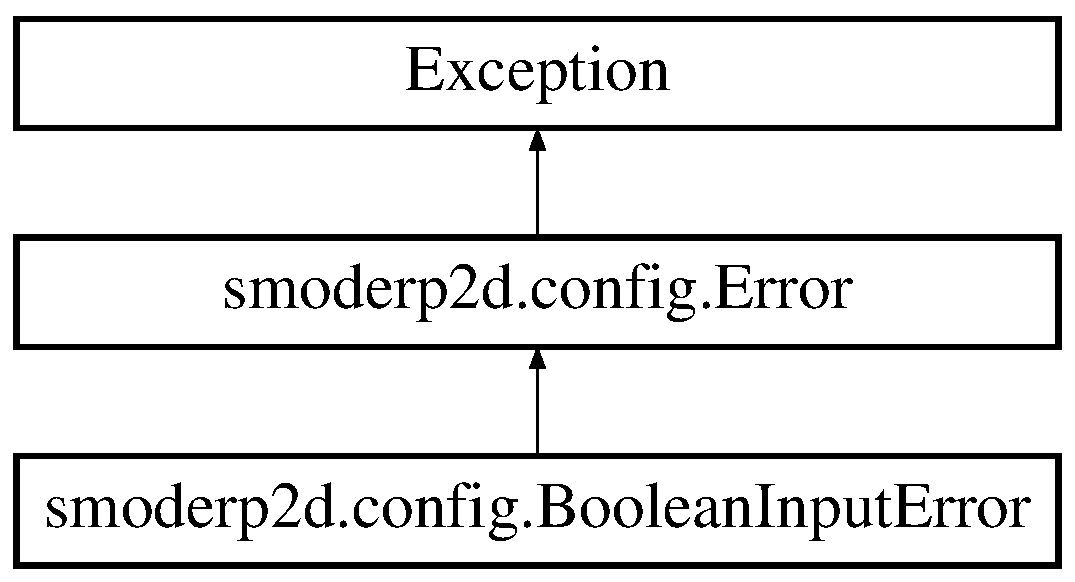
\includegraphics[height=3.000000cm]{classsmoderp2d_1_1config_1_1BooleanInputError}
\end{center}
\end{figure}
\subsection*{Public Member Functions}
\begin{DoxyCompactItemize}
\item 
\hypertarget{classsmoderp2d_1_1config_1_1BooleanInputError_a360baa4e5ed00b7e1be2f69c827bc744}{def {\bfseries \-\_\-\-\_\-init\-\_\-\-\_\-}}\label{classsmoderp2d_1_1config_1_1BooleanInputError_a360baa4e5ed00b7e1be2f69c827bc744}

\item 
\hypertarget{classsmoderp2d_1_1config_1_1BooleanInputError_a44476063da3a69ec01d9d0215fe03f17}{def {\bfseries \-\_\-\-\_\-str\-\_\-\-\_\-}}\label{classsmoderp2d_1_1config_1_1BooleanInputError_a44476063da3a69ec01d9d0215fe03f17}

\end{DoxyCompactItemize}
\subsection*{Public Attributes}
\begin{DoxyCompactItemize}
\item 
\hypertarget{classsmoderp2d_1_1config_1_1BooleanInputError_a4d9e5f70b1bb7cd8071adc203c15acc1}{{\bfseries msg}}\label{classsmoderp2d_1_1config_1_1BooleanInputError_a4d9e5f70b1bb7cd8071adc203c15acc1}

\end{DoxyCompactItemize}


\subsection{Detailed Description}
\begin{DoxyVerb}Exception raised for nonboolean value.

Attributes:
    msg  -- explanation of the error
\end{DoxyVerb}
 

The documentation for this class was generated from the following file\-:\begin{DoxyCompactItemize}
\item 
smoderp2d/config.\-py\end{DoxyCompactItemize}

\hypertarget{classsmoderp2d_1_1src_1_1courant_1_1Courant}{\section{smoderp2d.\-src.\-courant.\-Courant Class Reference}
\label{classsmoderp2d_1_1src_1_1courant_1_1Courant}\index{smoderp2d.\-src.\-courant.\-Courant@{smoderp2d.\-src.\-courant.\-Courant}}
}


Contains variables and methods needed for time step size handling.  


\subsection*{Public Member Functions}
\begin{DoxyCompactItemize}
\item 
\hypertarget{classsmoderp2d_1_1src_1_1courant_1_1Courant_a629841e2699d232acff8b2285dd1dcd7}{def \hyperlink{classsmoderp2d_1_1src_1_1courant_1_1Courant_a629841e2699d232acff8b2285dd1dcd7}{\-\_\-\-\_\-init\-\_\-\-\_\-}}\label{classsmoderp2d_1_1src_1_1courant_1_1Courant_a629841e2699d232acff8b2285dd1dcd7}

\begin{DoxyCompactList}\small\item\em constructor \end{DoxyCompactList}\item 
\hypertarget{classsmoderp2d_1_1src_1_1courant_1_1Courant_ae788349453919f497d8712ac4a8e12ef}{def \hyperlink{classsmoderp2d_1_1src_1_1courant_1_1Courant_ae788349453919f497d8712ac4a8e12ef}{set\-\_\-time\-\_\-step}}\label{classsmoderp2d_1_1src_1_1courant_1_1Courant_ae788349453919f497d8712ac4a8e12ef}

\begin{DoxyCompactList}\small\item\em Store the original guess time step. \end{DoxyCompactList}\item 
\hypertarget{classsmoderp2d_1_1src_1_1courant_1_1Courant_a9ebe11436dc1c1efa6c2a2f4fd2733f2}{def \hyperlink{classsmoderp2d_1_1src_1_1courant_1_1Courant_a9ebe11436dc1c1efa6c2a2f4fd2733f2}{reset}}\label{classsmoderp2d_1_1src_1_1courant_1_1Courant_a9ebe11436dc1c1efa6c2a2f4fd2733f2}

\begin{DoxyCompactList}\small\item\em Resets the self.\-cour\-\_\-most and self.\-cour\-\_\-speed after each time stop computation is successfully completed. \end{DoxyCompactList}\item 
def \hyperlink{classsmoderp2d_1_1src_1_1courant_1_1Courant_ab69d95fbe66467f71b0a535be611f05b}{initial\-\_\-time\-\_\-step}
\begin{DoxyCompactList}\small\item\em Guesses the initial time step. \end{DoxyCompactList}\item 
\hypertarget{classsmoderp2d_1_1src_1_1courant_1_1Courant_a80d541950a9e78a273f8145e4ea76f3b}{def \hyperlink{classsmoderp2d_1_1src_1_1courant_1_1Courant_a80d541950a9e78a273f8145e4ea76f3b}{C\-F\-L}}\label{classsmoderp2d_1_1src_1_1courant_1_1Courant_a80d541950a9e78a273f8145e4ea76f3b}

\begin{DoxyCompactList}\small\item\em Checks and store in each computational cell the maximum velocity and maximum \hyperlink{classsmoderp2d_1_1src_1_1courant_1_1Courant}{Courant} coefficient. \end{DoxyCompactList}\item 
def \hyperlink{classsmoderp2d_1_1src_1_1courant_1_1Courant_a6a20926e1f36e2169eccdc27d92d787d}{courant}
\begin{DoxyCompactList}\small\item\em Returns the adjusted/unchanged time step after a time step computation is completed. \end{DoxyCompactList}\end{DoxyCompactItemize}
\subsection*{Public Attributes}
\begin{DoxyCompactItemize}
\item 
\hypertarget{classsmoderp2d_1_1src_1_1courant_1_1Courant_a7f7b7ef10ca7fd66b190379cea4203d3}{{\bfseries maxh}}\label{classsmoderp2d_1_1src_1_1courant_1_1Courant_a7f7b7ef10ca7fd66b190379cea4203d3}

\item 
\hypertarget{classsmoderp2d_1_1src_1_1courant_1_1Courant_a2e4c6d74b15eb45d67ebba896b97eb32}{{\bfseries cour\-\_\-speed}}\label{classsmoderp2d_1_1src_1_1courant_1_1Courant_a2e4c6d74b15eb45d67ebba896b97eb32}

\item 
\hypertarget{classsmoderp2d_1_1src_1_1courant_1_1Courant_a059271cdbd6044635ad290eadff9299b}{\hyperlink{classsmoderp2d_1_1src_1_1courant_1_1Courant_a059271cdbd6044635ad290eadff9299b}{cour\-\_\-crit}}\label{classsmoderp2d_1_1src_1_1courant_1_1Courant_a059271cdbd6044635ad290eadff9299b}

\begin{DoxyCompactList}\small\item\em citical courant value \end{DoxyCompactList}\item 
\hypertarget{classsmoderp2d_1_1src_1_1courant_1_1Courant_afa3e7bde711d11925d54a41ecffdc2f3}{{\bfseries cour\-\_\-most}}\label{classsmoderp2d_1_1src_1_1courant_1_1Courant_afa3e7bde711d11925d54a41ecffdc2f3}

\item 
\hypertarget{classsmoderp2d_1_1src_1_1courant_1_1Courant_a2bfcce1ddcb5060045dbd777c848c9f2}{{\bfseries cour\-\_\-most\-\_\-rill}}\label{classsmoderp2d_1_1src_1_1courant_1_1Courant_a2bfcce1ddcb5060045dbd777c848c9f2}

\item 
\hypertarget{classsmoderp2d_1_1src_1_1courant_1_1Courant_ae0eb94299899733aa39b68e166115809}{{\bfseries cour\-\_\-coef}}\label{classsmoderp2d_1_1src_1_1courant_1_1Courant_ae0eb94299899733aa39b68e166115809}

\item 
\hypertarget{classsmoderp2d_1_1src_1_1courant_1_1Courant_a87b5aad2d2f85e4af9046d7ea40913c8}{{\bfseries cour\-\_\-least}}\label{classsmoderp2d_1_1src_1_1courant_1_1Courant_a87b5aad2d2f85e4af9046d7ea40913c8}

\item 
\hypertarget{classsmoderp2d_1_1src_1_1courant_1_1Courant_a60a04e01f0bc1843a65eddcb7c388b6c}{{\bfseries i}}\label{classsmoderp2d_1_1src_1_1courant_1_1Courant_a60a04e01f0bc1843a65eddcb7c388b6c}

\item 
\hypertarget{classsmoderp2d_1_1src_1_1courant_1_1Courant_ad7980557f43390dbafa7a32c2eb5587f}{{\bfseries j}}\label{classsmoderp2d_1_1src_1_1courant_1_1Courant_ad7980557f43390dbafa7a32c2eb5587f}

\item 
\hypertarget{classsmoderp2d_1_1src_1_1courant_1_1Courant_a1ce8167e370399dae153ffac1a9506cd}{{\bfseries co}}\label{classsmoderp2d_1_1src_1_1courant_1_1Courant_a1ce8167e370399dae153ffac1a9506cd}

\item 
\hypertarget{classsmoderp2d_1_1src_1_1courant_1_1Courant_ad30d2f98a2d53cac3e07e7e0b3cedd39}{{\bfseries co\-\_\-pre}}\label{classsmoderp2d_1_1src_1_1courant_1_1Courant_ad30d2f98a2d53cac3e07e7e0b3cedd39}

\item 
\hypertarget{classsmoderp2d_1_1src_1_1courant_1_1Courant_aca2e98eb52dc3dcd664209462b181ba1}{{\bfseries maxratio}}\label{classsmoderp2d_1_1src_1_1courant_1_1Courant_aca2e98eb52dc3dcd664209462b181ba1}

\item 
\hypertarget{classsmoderp2d_1_1src_1_1courant_1_1Courant_a03e5161b202d6d9ecaa2ab6bc2f6364c}{{\bfseries max\-\_\-delta\-\_\-t}}\label{classsmoderp2d_1_1src_1_1courant_1_1Courant_a03e5161b202d6d9ecaa2ab6bc2f6364c}

\item 
\hypertarget{classsmoderp2d_1_1src_1_1courant_1_1Courant_a4cd64dfec3bd294d881fd28581250b45}{{\bfseries max\-\_\-delta\-\_\-t\-\_\-mult}}\label{classsmoderp2d_1_1src_1_1courant_1_1Courant_a4cd64dfec3bd294d881fd28581250b45}

\item 
\hypertarget{classsmoderp2d_1_1src_1_1courant_1_1Courant_ae5af3c6c7c3c4a048d92af266d8abeca}{{\bfseries orig\-\_\-dt}}\label{classsmoderp2d_1_1src_1_1courant_1_1Courant_ae5af3c6c7c3c4a048d92af266d8abeca}

\end{DoxyCompactItemize}


\subsection{Detailed Description}
Contains variables and methods needed for time step size handling. 



\subsection{Member Function Documentation}
\hypertarget{classsmoderp2d_1_1src_1_1courant_1_1Courant_a6a20926e1f36e2169eccdc27d92d787d}{\index{smoderp2d\-::src\-::courant\-::\-Courant@{smoderp2d\-::src\-::courant\-::\-Courant}!courant@{courant}}
\index{courant@{courant}!smoderp2d::src::courant::Courant@{smoderp2d\-::src\-::courant\-::\-Courant}}
\subsubsection[{courant}]{\setlength{\rightskip}{0pt plus 5cm}def smoderp2d.\-src.\-courant.\-Courant.\-courant (
\begin{DoxyParamCaption}
\item[{}]{self, }
\item[{}]{rainfall, }
\item[{}]{delta\-\_\-t, }
\item[{}]{efect\-\_\-vrst, }
\item[{}]{ratio}
\end{DoxyParamCaption}
)}}\label{classsmoderp2d_1_1src_1_1courant_1_1Courant_a6a20926e1f36e2169eccdc27d92d787d}


Returns the adjusted/unchanged time step after a time step computation is completed. 

Also returns the ratio for the rill computation division. if ((ratio $>$ self.\-maxratio) or (self.\-cour\-\_\-most\-\_\-rill $>$ 1.\-0)) \-: ratio = self.\-maxratio ratio = 1 self.\-max\-\_\-delta\-\_\-t\-\_\-mult $\ast$= 0.\-9 \hypertarget{classsmoderp2d_1_1src_1_1courant_1_1Courant_ab69d95fbe66467f71b0a535be611f05b}{\index{smoderp2d\-::src\-::courant\-::\-Courant@{smoderp2d\-::src\-::courant\-::\-Courant}!initial\-\_\-time\-\_\-step@{initial\-\_\-time\-\_\-step}}
\index{initial\-\_\-time\-\_\-step@{initial\-\_\-time\-\_\-step}!smoderp2d::src::courant::Courant@{smoderp2d\-::src\-::courant\-::\-Courant}}
\subsubsection[{initial\-\_\-time\-\_\-step}]{\setlength{\rightskip}{0pt plus 5cm}def smoderp2d.\-src.\-courant.\-Courant.\-initial\-\_\-time\-\_\-step (
\begin{DoxyParamCaption}
\item[{}]{self, }
\item[{}]{sur}
\end{DoxyParamCaption}
)}}\label{classsmoderp2d_1_1src_1_1courant_1_1Courant_ab69d95fbe66467f71b0a535be611f05b}


Guesses the initial time step. 

the guess is based on the maximum {\itshape a} and {\itshape b} parameters of the kinematic wave equation and critical water level in case of sheet flow only calculation the water level guess is 0.\-001 {\itshape m} by default 

The documentation for this class was generated from the following file\-:\begin{DoxyCompactItemize}
\item 
smoderp2d/src/courant.\-py\end{DoxyCompactItemize}

\hypertarget{classsmoderp2d_1_1src_1_1io__functions_1_1progress__bar_1_1CPROG}{\section{smoderp2d.\-src.\-io\-\_\-functions.\-progress\-\_\-bar.\-C\-P\-R\-O\-G Class Reference}
\label{classsmoderp2d_1_1src_1_1io__functions_1_1progress__bar_1_1CPROG}\index{smoderp2d.\-src.\-io\-\_\-functions.\-progress\-\_\-bar.\-C\-P\-R\-O\-G@{smoderp2d.\-src.\-io\-\_\-functions.\-progress\-\_\-bar.\-C\-P\-R\-O\-G}}
}
\subsection*{Public Member Functions}
\begin{DoxyCompactItemize}
\item 
\hypertarget{classsmoderp2d_1_1src_1_1io__functions_1_1progress__bar_1_1CPROG_ab17498ec58d6a6a8da846fe178dda15a}{def {\bfseries \-\_\-\-\_\-init\-\_\-\-\_\-}}\label{classsmoderp2d_1_1src_1_1io__functions_1_1progress__bar_1_1CPROG_ab17498ec58d6a6a8da846fe178dda15a}

\item 
\hypertarget{classsmoderp2d_1_1src_1_1io__functions_1_1progress__bar_1_1CPROG_aed7dbe1604e19325619d67dece13f994}{def {\bfseries update}}\label{classsmoderp2d_1_1src_1_1io__functions_1_1progress__bar_1_1CPROG_aed7dbe1604e19325619d67dece13f994}

\end{DoxyCompactItemize}
\subsection*{Public Attributes}
\begin{DoxyCompactItemize}
\item 
\hypertarget{classsmoderp2d_1_1src_1_1io__functions_1_1progress__bar_1_1CPROG_af8242685ed25599ff6320b17d7ecc97f}{\hyperlink{classsmoderp2d_1_1src_1_1io__functions_1_1progress__bar_1_1CPROG_af8242685ed25599ff6320b17d7ecc97f}{pre}}\label{classsmoderp2d_1_1src_1_1io__functions_1_1progress__bar_1_1CPROG_af8242685ed25599ff6320b17d7ecc97f}

\begin{DoxyCompactList}\small\item\em print i i = round(i) \end{DoxyCompactList}\item 
\hypertarget{classsmoderp2d_1_1src_1_1io__functions_1_1progress__bar_1_1CPROG_ae43bff15d5e6b6571009fc2459e7d9a4}{{\bfseries start\-Time}}\label{classsmoderp2d_1_1src_1_1io__functions_1_1progress__bar_1_1CPROG_ae43bff15d5e6b6571009fc2459e7d9a4}

\item 
\hypertarget{classsmoderp2d_1_1src_1_1io__functions_1_1progress__bar_1_1CPROG_aa437f963e707b59285914615876cd745}{{\bfseries curr\-Time}}\label{classsmoderp2d_1_1src_1_1io__functions_1_1progress__bar_1_1CPROG_aa437f963e707b59285914615876cd745}

\end{DoxyCompactItemize}


\subsection{Detailed Description}


Definition at line 21 of file progress\-\_\-bar.\-py.



The documentation for this class was generated from the following file\-:\begin{DoxyCompactItemize}
\item 
smoderp2d/src/io\-\_\-functions/progress\-\_\-bar.\-py\end{DoxyCompactItemize}

\hypertarget{classsmoderp2d_1_1src_1_1main__classes_1_1CumulativeMax_1_1Cumulative}{\section{smoderp2d.\-src.\-main\-\_\-classes.\-Cumulative\-Max.\-Cumulative Class Reference}
\label{classsmoderp2d_1_1src_1_1main__classes_1_1CumulativeMax_1_1Cumulative}\index{smoderp2d.\-src.\-main\-\_\-classes.\-Cumulative\-Max.\-Cumulative@{smoderp2d.\-src.\-main\-\_\-classes.\-Cumulative\-Max.\-Cumulative}}
}


Max and \hyperlink{classsmoderp2d_1_1src_1_1main__classes_1_1CumulativeMax_1_1Cumulative}{Cumulative} values.  


Inheritance diagram for smoderp2d.\-src.\-main\-\_\-classes.\-Cumulative\-Max.\-Cumulative\-:\begin{figure}[H]
\begin{center}
\leavevmode
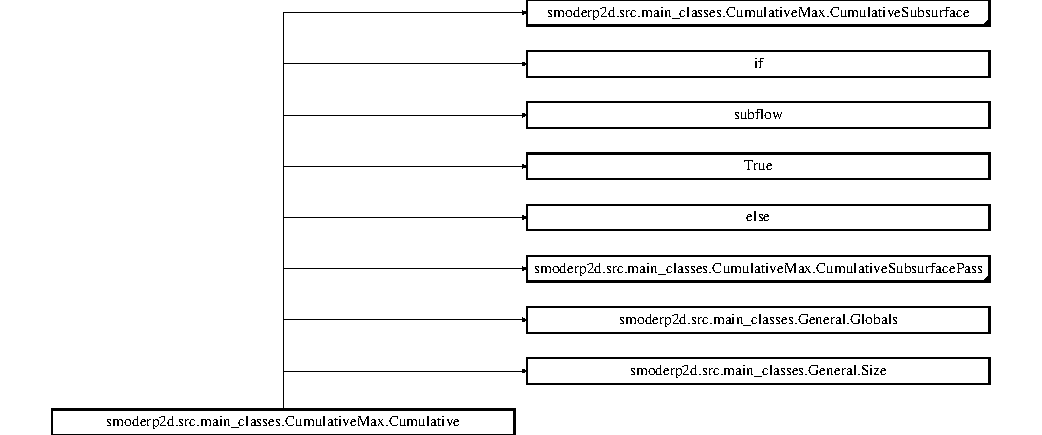
\includegraphics[height=5.846868cm]{classsmoderp2d_1_1src_1_1main__classes_1_1CumulativeMax_1_1Cumulative}
\end{center}
\end{figure}
\subsection*{Public Member Functions}
\begin{DoxyCompactItemize}
\item 
def \hyperlink{classsmoderp2d_1_1src_1_1main__classes_1_1CumulativeMax_1_1Cumulative_aa0e7706be42a1c06b1861c1e8c100c4c}{\-\_\-\-\_\-init\-\_\-\-\_\-}
\begin{DoxyCompactList}\small\item\em the constructor \end{DoxyCompactList}\item 
def \hyperlink{classsmoderp2d_1_1src_1_1main__classes_1_1CumulativeMax_1_1Cumulative_a8ff1f325481804578ec1cdc47616a808}{update\-\_\-cumulative}
\begin{DoxyCompactList}\small\item\em Method is used after each time step to save the desired variables. \end{DoxyCompactList}\end{DoxyCompactItemize}
\subsection*{Public Attributes}
\begin{DoxyCompactItemize}
\item 
\hyperlink{classsmoderp2d_1_1src_1_1main__classes_1_1CumulativeMax_1_1Cumulative_a55debe509dff6cac1e187511891e8ca6}{arrs}
\begin{DoxyCompactList}\small\item\em Dictionary stores the python arrays identification. \end{DoxyCompactList}\item 
\hyperlink{classsmoderp2d_1_1src_1_1main__classes_1_1CumulativeMax_1_1Cumulative_a5c371c6f6e52bbd3ac4545f7bbe87bd3}{names}
\begin{DoxyCompactList}\small\item\em Dictionary stores the the arrays name used in the output rasters. \end{DoxyCompactList}\item 
\hypertarget{classsmoderp2d_1_1src_1_1main__classes_1_1CumulativeMax_1_1Cumulative_ae4f8a2ce74c1284f06037cf0a28ec4c7}{\hyperlink{classsmoderp2d_1_1src_1_1main__classes_1_1CumulativeMax_1_1Cumulative_ae4f8a2ce74c1284f06037cf0a28ec4c7}{n}}\label{classsmoderp2d_1_1src_1_1main__classes_1_1CumulativeMax_1_1Cumulative_ae4f8a2ce74c1284f06037cf0a28ec4c7}

\begin{DoxyCompactList}\small\item\em array count stored in the class \end{DoxyCompactList}\item 
\hypertarget{classsmoderp2d_1_1src_1_1main__classes_1_1CumulativeMax_1_1Cumulative_a2d35535475955e365c555506003ed956}{\hyperlink{classsmoderp2d_1_1src_1_1main__classes_1_1CumulativeMax_1_1Cumulative_a2d35535475955e365c555506003ed956}{infiltration}}\label{classsmoderp2d_1_1src_1_1main__classes_1_1CumulativeMax_1_1Cumulative_a2d35535475955e365c555506003ed956}

\begin{DoxyCompactList}\small\item\em cumulative infiltrated volume \mbox{[}m3\mbox{]} \end{DoxyCompactList}\item 
\hypertarget{classsmoderp2d_1_1src_1_1main__classes_1_1CumulativeMax_1_1Cumulative_ab1532dc55bfb6a69559fbc6639c89de6}{\hyperlink{classsmoderp2d_1_1src_1_1main__classes_1_1CumulativeMax_1_1Cumulative_ab1532dc55bfb6a69559fbc6639c89de6}{precipitation}}\label{classsmoderp2d_1_1src_1_1main__classes_1_1CumulativeMax_1_1Cumulative_ab1532dc55bfb6a69559fbc6639c89de6}

\begin{DoxyCompactList}\small\item\em cumulative precipitation volume \mbox{[}m3\mbox{]} \end{DoxyCompactList}\item 
\hypertarget{classsmoderp2d_1_1src_1_1main__classes_1_1CumulativeMax_1_1Cumulative_a3f1bfdea16273c1d526adf267f151b8f}{\hyperlink{classsmoderp2d_1_1src_1_1main__classes_1_1CumulativeMax_1_1Cumulative_a3f1bfdea16273c1d526adf267f151b8f}{h\-\_\-sur}}\label{classsmoderp2d_1_1src_1_1main__classes_1_1CumulativeMax_1_1Cumulative_a3f1bfdea16273c1d526adf267f151b8f}

\begin{DoxyCompactList}\small\item\em maximum surface water level \mbox{[}m\mbox{]} \end{DoxyCompactList}\item 
\hypertarget{classsmoderp2d_1_1src_1_1main__classes_1_1CumulativeMax_1_1Cumulative_a638db7f8604658dc1e148a06019ae2b5}{\hyperlink{classsmoderp2d_1_1src_1_1main__classes_1_1CumulativeMax_1_1Cumulative_a638db7f8604658dc1e148a06019ae2b5}{q\-\_\-sur}}\label{classsmoderp2d_1_1src_1_1main__classes_1_1CumulativeMax_1_1Cumulative_a638db7f8604658dc1e148a06019ae2b5}

\begin{DoxyCompactList}\small\item\em maximum surface discharge \mbox{[}m3s-\/1\mbox{]} \end{DoxyCompactList}\item 
\hypertarget{classsmoderp2d_1_1src_1_1main__classes_1_1CumulativeMax_1_1Cumulative_a5dba2fc38132916c8a27ba3181cc5abe}{\hyperlink{classsmoderp2d_1_1src_1_1main__classes_1_1CumulativeMax_1_1Cumulative_a5dba2fc38132916c8a27ba3181cc5abe}{V\-\_\-sur}}\label{classsmoderp2d_1_1src_1_1main__classes_1_1CumulativeMax_1_1Cumulative_a5dba2fc38132916c8a27ba3181cc5abe}

\begin{DoxyCompactList}\small\item\em cumulative surface runoff volume \mbox{[}m3\mbox{]} \end{DoxyCompactList}\item 
\hypertarget{classsmoderp2d_1_1src_1_1main__classes_1_1CumulativeMax_1_1Cumulative_a6022a0431a925ed744c88ec683aec526}{\hyperlink{classsmoderp2d_1_1src_1_1main__classes_1_1CumulativeMax_1_1Cumulative_a6022a0431a925ed744c88ec683aec526}{V\-\_\-sur\-\_\-r}}\label{classsmoderp2d_1_1src_1_1main__classes_1_1CumulativeMax_1_1Cumulative_a6022a0431a925ed744c88ec683aec526}

\begin{DoxyCompactList}\small\item\em cumulative surface runoff volume \mbox{[}m3\mbox{]} \end{DoxyCompactList}\item 
\hypertarget{classsmoderp2d_1_1src_1_1main__classes_1_1CumulativeMax_1_1Cumulative_ae7d8b3364672d4cc58a69515441b65fe}{\hyperlink{classsmoderp2d_1_1src_1_1main__classes_1_1CumulativeMax_1_1Cumulative_ae7d8b3364672d4cc58a69515441b65fe}{v\-\_\-sur}}\label{classsmoderp2d_1_1src_1_1main__classes_1_1CumulativeMax_1_1Cumulative_ae7d8b3364672d4cc58a69515441b65fe}

\begin{DoxyCompactList}\small\item\em maximum surface velocity \mbox{[}ms-\/1\mbox{]} \end{DoxyCompactList}\item 
\hypertarget{classsmoderp2d_1_1src_1_1main__classes_1_1CumulativeMax_1_1Cumulative_a5a77d63173ad36d599b00f21d0d2f109}{\hyperlink{classsmoderp2d_1_1src_1_1main__classes_1_1CumulativeMax_1_1Cumulative_a5a77d63173ad36d599b00f21d0d2f109}{shear\-\_\-sur}}\label{classsmoderp2d_1_1src_1_1main__classes_1_1CumulativeMax_1_1Cumulative_a5a77d63173ad36d599b00f21d0d2f109}

\begin{DoxyCompactList}\small\item\em maximum surface shear stress \mbox{[}Pa\mbox{]} \end{DoxyCompactList}\item 
\hypertarget{classsmoderp2d_1_1src_1_1main__classes_1_1CumulativeMax_1_1Cumulative_a6eac6988b76e8fb592a2fe73254a487f}{\hyperlink{classsmoderp2d_1_1src_1_1main__classes_1_1CumulativeMax_1_1Cumulative_a6eac6988b76e8fb592a2fe73254a487f}{inflow\-\_\-sur}}\label{classsmoderp2d_1_1src_1_1main__classes_1_1CumulativeMax_1_1Cumulative_a6eac6988b76e8fb592a2fe73254a487f}

\begin{DoxyCompactList}\small\item\em cumulative surface inflow volume \mbox{[}m3\mbox{]} \end{DoxyCompactList}\item 
\hypertarget{classsmoderp2d_1_1src_1_1main__classes_1_1CumulativeMax_1_1Cumulative_a051fee65df3eaa945e2704cc9e1ec159}{\hyperlink{classsmoderp2d_1_1src_1_1main__classes_1_1CumulativeMax_1_1Cumulative_a051fee65df3eaa945e2704cc9e1ec159}{h\-\_\-rill}}\label{classsmoderp2d_1_1src_1_1main__classes_1_1CumulativeMax_1_1Cumulative_a051fee65df3eaa945e2704cc9e1ec159}

\begin{DoxyCompactList}\small\item\em maximum water level in rills \mbox{[}m\mbox{]} \end{DoxyCompactList}\item 
\hypertarget{classsmoderp2d_1_1src_1_1main__classes_1_1CumulativeMax_1_1Cumulative_a74582962ffa39d74cafe5ba723ad38ea}{\hyperlink{classsmoderp2d_1_1src_1_1main__classes_1_1CumulativeMax_1_1Cumulative_a74582962ffa39d74cafe5ba723ad38ea}{q\-\_\-rill}}\label{classsmoderp2d_1_1src_1_1main__classes_1_1CumulativeMax_1_1Cumulative_a74582962ffa39d74cafe5ba723ad38ea}

\begin{DoxyCompactList}\small\item\em maximum discharge in rills \mbox{[}m3s-\/1\mbox{]} \end{DoxyCompactList}\item 
\hypertarget{classsmoderp2d_1_1src_1_1main__classes_1_1CumulativeMax_1_1Cumulative_aa41ba52604c60795f131a41ebfa45025}{\hyperlink{classsmoderp2d_1_1src_1_1main__classes_1_1CumulativeMax_1_1Cumulative_aa41ba52604c60795f131a41ebfa45025}{V\-\_\-rill}}\label{classsmoderp2d_1_1src_1_1main__classes_1_1CumulativeMax_1_1Cumulative_aa41ba52604c60795f131a41ebfa45025}

\begin{DoxyCompactList}\small\item\em cumulative runoff volume in rills \mbox{[}m3\mbox{]} \end{DoxyCompactList}\item 
\hypertarget{classsmoderp2d_1_1src_1_1main__classes_1_1CumulativeMax_1_1Cumulative_a3301f1f27bfd5ad1548b3c478759fe27}{\hyperlink{classsmoderp2d_1_1src_1_1main__classes_1_1CumulativeMax_1_1Cumulative_a3301f1f27bfd5ad1548b3c478759fe27}{V\-\_\-rill\-\_\-r}}\label{classsmoderp2d_1_1src_1_1main__classes_1_1CumulativeMax_1_1Cumulative_a3301f1f27bfd5ad1548b3c478759fe27}

\begin{DoxyCompactList}\small\item\em cumulative runoff volume in rills \mbox{[}m3\mbox{]} \end{DoxyCompactList}\item 
\hypertarget{classsmoderp2d_1_1src_1_1main__classes_1_1CumulativeMax_1_1Cumulative_a16689860237806fdcb41b2e66f8961ec}{\hyperlink{classsmoderp2d_1_1src_1_1main__classes_1_1CumulativeMax_1_1Cumulative_a16689860237806fdcb41b2e66f8961ec}{b\-\_\-rill}}\label{classsmoderp2d_1_1src_1_1main__classes_1_1CumulativeMax_1_1Cumulative_a16689860237806fdcb41b2e66f8961ec}

\begin{DoxyCompactList}\small\item\em maximum rill width \mbox{[}m\mbox{]} \end{DoxyCompactList}\item 
\hypertarget{classsmoderp2d_1_1src_1_1main__classes_1_1CumulativeMax_1_1Cumulative_a362df44a6e225a24274bb136ffb07a90}{\hyperlink{classsmoderp2d_1_1src_1_1main__classes_1_1CumulativeMax_1_1Cumulative_a362df44a6e225a24274bb136ffb07a90}{v\-\_\-rill}}\label{classsmoderp2d_1_1src_1_1main__classes_1_1CumulativeMax_1_1Cumulative_a362df44a6e225a24274bb136ffb07a90}

\begin{DoxyCompactList}\small\item\em maximum velocity in rills \mbox{[}ms-\/1\mbox{]} \end{DoxyCompactList}\item 
\hypertarget{classsmoderp2d_1_1src_1_1main__classes_1_1CumulativeMax_1_1Cumulative_adff5e628465be89b7d4dcafe819c90c6}{\hyperlink{classsmoderp2d_1_1src_1_1main__classes_1_1CumulativeMax_1_1Cumulative_adff5e628465be89b7d4dcafe819c90c6}{sur\-\_\-ret}}\label{classsmoderp2d_1_1src_1_1main__classes_1_1CumulativeMax_1_1Cumulative_adff5e628465be89b7d4dcafe819c90c6}

\begin{DoxyCompactList}\small\item\em maximum surface retention \mbox{[}m\mbox{]} \end{DoxyCompactList}\item 
\hypertarget{classsmoderp2d_1_1src_1_1main__classes_1_1CumulativeMax_1_1Cumulative_a5fc3db54d59c21cd0b771f3778fede7c}{\hyperlink{classsmoderp2d_1_1src_1_1main__classes_1_1CumulativeMax_1_1Cumulative_a5fc3db54d59c21cd0b771f3778fede7c}{q\-\_\-sur\-\_\-tot}}\label{classsmoderp2d_1_1src_1_1main__classes_1_1CumulativeMax_1_1Cumulative_a5fc3db54d59c21cd0b771f3778fede7c}

\begin{DoxyCompactList}\small\item\em maximal total surface flow \mbox{[}m3/s\mbox{]} \end{DoxyCompactList}\item 
\hypertarget{classsmoderp2d_1_1src_1_1main__classes_1_1CumulativeMax_1_1Cumulative_a79fde62f00a019dcad258bf8c819312e}{\hyperlink{classsmoderp2d_1_1src_1_1main__classes_1_1CumulativeMax_1_1Cumulative_a79fde62f00a019dcad258bf8c819312e}{V\-\_\-sur\-\_\-tot}}\label{classsmoderp2d_1_1src_1_1main__classes_1_1CumulativeMax_1_1Cumulative_a79fde62f00a019dcad258bf8c819312e}

\begin{DoxyCompactList}\small\item\em cumulative total surface flow \mbox{[}m3/s\mbox{]} \end{DoxyCompactList}\end{DoxyCompactItemize}
\subsection*{Additional Inherited Members}


\subsection{Detailed Description}
Max and \hyperlink{classsmoderp2d_1_1src_1_1main__classes_1_1CumulativeMax_1_1Cumulative}{Cumulative} values. 

Stores array of max or cumulative values at of important variables from the surface and rill flow 

\subsection{Constructor \& Destructor Documentation}
\hypertarget{classsmoderp2d_1_1src_1_1main__classes_1_1CumulativeMax_1_1Cumulative_aa0e7706be42a1c06b1861c1e8c100c4c}{\index{smoderp2d\-::src\-::main\-\_\-classes\-::\-Cumulative\-Max\-::\-Cumulative@{smoderp2d\-::src\-::main\-\_\-classes\-::\-Cumulative\-Max\-::\-Cumulative}!\-\_\-\-\_\-init\-\_\-\-\_\-@{\-\_\-\-\_\-init\-\_\-\-\_\-}}
\index{\-\_\-\-\_\-init\-\_\-\-\_\-@{\-\_\-\-\_\-init\-\_\-\-\_\-}!smoderp2d::src::main_classes::CumulativeMax::Cumulative@{smoderp2d\-::src\-::main\-\_\-classes\-::\-Cumulative\-Max\-::\-Cumulative}}
\subsubsection[{\-\_\-\-\_\-init\-\_\-\-\_\-}]{\setlength{\rightskip}{0pt plus 5cm}def smoderp2d.\-src.\-main\-\_\-classes.\-Cumulative\-Max.\-Cumulative.\-\_\-\-\_\-init\-\_\-\-\_\- (
\begin{DoxyParamCaption}
\item[{}]{self}
\end{DoxyParamCaption}
)}}\label{classsmoderp2d_1_1src_1_1main__classes_1_1CumulativeMax_1_1Cumulative_aa0e7706be42a1c06b1861c1e8c100c4c}


the constructor 



\subsection{Member Function Documentation}
\hypertarget{classsmoderp2d_1_1src_1_1main__classes_1_1CumulativeMax_1_1Cumulative_a8ff1f325481804578ec1cdc47616a808}{\index{smoderp2d\-::src\-::main\-\_\-classes\-::\-Cumulative\-Max\-::\-Cumulative@{smoderp2d\-::src\-::main\-\_\-classes\-::\-Cumulative\-Max\-::\-Cumulative}!update\-\_\-cumulative@{update\-\_\-cumulative}}
\index{update\-\_\-cumulative@{update\-\_\-cumulative}!smoderp2d::src::main_classes::CumulativeMax::Cumulative@{smoderp2d\-::src\-::main\-\_\-classes\-::\-Cumulative\-Max\-::\-Cumulative}}
\subsubsection[{update\-\_\-cumulative}]{\setlength{\rightskip}{0pt plus 5cm}def smoderp2d.\-src.\-main\-\_\-classes.\-Cumulative\-Max.\-Cumulative.\-update\-\_\-cumulative (
\begin{DoxyParamCaption}
\item[{}]{self, }
\item[{}]{i, }
\item[{}]{j, }
\item[{}]{surface, }
\item[{}]{subsurface, }
\item[{}]{delta\-\_\-t}
\end{DoxyParamCaption}
)}}\label{classsmoderp2d_1_1src_1_1main__classes_1_1CumulativeMax_1_1Cumulative_a8ff1f325481804578ec1cdc47616a808}


Method is used after each time step to save the desired variables. 

Method is called in \hyperlink{namespacesmoderp2d_1_1src_1_1runoff}{smoderp2d.\-src.\-runoff} 

\subsection{Member Data Documentation}
\hypertarget{classsmoderp2d_1_1src_1_1main__classes_1_1CumulativeMax_1_1Cumulative_a55debe509dff6cac1e187511891e8ca6}{\index{smoderp2d\-::src\-::main\-\_\-classes\-::\-Cumulative\-Max\-::\-Cumulative@{smoderp2d\-::src\-::main\-\_\-classes\-::\-Cumulative\-Max\-::\-Cumulative}!arrs@{arrs}}
\index{arrs@{arrs}!smoderp2d::src::main_classes::CumulativeMax::Cumulative@{smoderp2d\-::src\-::main\-\_\-classes\-::\-Cumulative\-Max\-::\-Cumulative}}
\subsubsection[{arrs}]{\setlength{\rightskip}{0pt plus 5cm}smoderp2d.\-src.\-main\-\_\-classes.\-Cumulative\-Max.\-Cumulative.\-arrs}}\label{classsmoderp2d_1_1src_1_1main__classes_1_1CumulativeMax_1_1Cumulative_a55debe509dff6cac1e187511891e8ca6}


Dictionary stores the python arrays identification. 

self.\-arr is used in the smoderp2d.\-src.\-io\-\_\-functions.\-post\-\_\-proc \hypertarget{classsmoderp2d_1_1src_1_1main__classes_1_1CumulativeMax_1_1Cumulative_a5c371c6f6e52bbd3ac4545f7bbe87bd3}{\index{smoderp2d\-::src\-::main\-\_\-classes\-::\-Cumulative\-Max\-::\-Cumulative@{smoderp2d\-::src\-::main\-\_\-classes\-::\-Cumulative\-Max\-::\-Cumulative}!names@{names}}
\index{names@{names}!smoderp2d::src::main_classes::CumulativeMax::Cumulative@{smoderp2d\-::src\-::main\-\_\-classes\-::\-Cumulative\-Max\-::\-Cumulative}}
\subsubsection[{names}]{\setlength{\rightskip}{0pt plus 5cm}smoderp2d.\-src.\-main\-\_\-classes.\-Cumulative\-Max.\-Cumulative.\-names}}\label{classsmoderp2d_1_1src_1_1main__classes_1_1CumulativeMax_1_1Cumulative_a5c371c6f6e52bbd3ac4545f7bbe87bd3}


Dictionary stores the the arrays name used in the output rasters. 

self.\-names is used in the smoderp2d.\-src.\-io\-\_\-functions.\-post\-\_\-proc 

The documentation for this class was generated from the following file\-:\begin{DoxyCompactItemize}
\item 
smoderp2d/src/main\-\_\-classes/Cumulative\-Max.\-py\end{DoxyCompactItemize}

\hypertarget{classsmoderp2d_1_1src_1_1main__classes_1_1CumulativeMax_1_1CumulativeSubsurface}{\section{smoderp2d.\-src.\-main\-\_\-classes.\-Cumulative\-Max.\-Cumulative\-Subsurface Class Reference}
\label{classsmoderp2d_1_1src_1_1main__classes_1_1CumulativeMax_1_1CumulativeSubsurface}\index{smoderp2d.\-src.\-main\-\_\-classes.\-Cumulative\-Max.\-Cumulative\-Subsurface@{smoderp2d.\-src.\-main\-\_\-classes.\-Cumulative\-Max.\-Cumulative\-Subsurface}}
}


Max and cumulative values of the subsurface flow.  


Inheritance diagram for smoderp2d.\-src.\-main\-\_\-classes.\-Cumulative\-Max.\-Cumulative\-Subsurface\-:\begin{figure}[H]
\begin{center}
\leavevmode
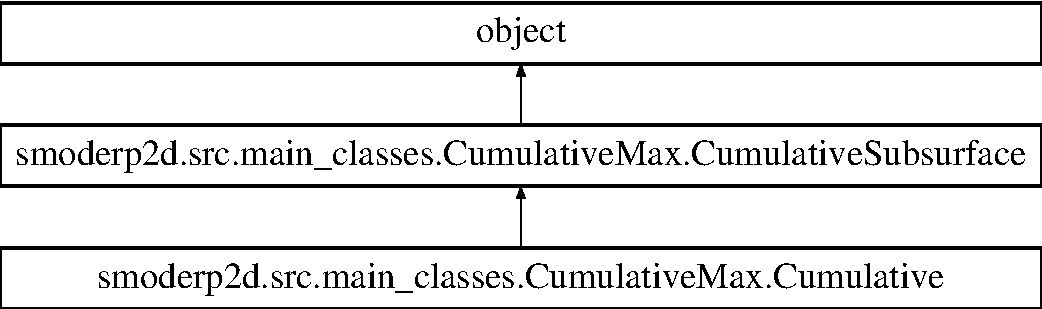
\includegraphics[height=3.000000cm]{classsmoderp2d_1_1src_1_1main__classes_1_1CumulativeMax_1_1CumulativeSubsurface}
\end{center}
\end{figure}
\subsection*{Public Member Functions}
\begin{DoxyCompactItemize}
\item 
\hypertarget{classsmoderp2d_1_1src_1_1main__classes_1_1CumulativeMax_1_1CumulativeSubsurface_a1c6651aa035dc033023bd0e88a7b795c}{def \hyperlink{classsmoderp2d_1_1src_1_1main__classes_1_1CumulativeMax_1_1CumulativeSubsurface_a1c6651aa035dc033023bd0e88a7b795c}{\-\_\-\-\_\-init\-\_\-\-\_\-}}\label{classsmoderp2d_1_1src_1_1main__classes_1_1CumulativeMax_1_1CumulativeSubsurface_a1c6651aa035dc033023bd0e88a7b795c}

\begin{DoxyCompactList}\small\item\em constructor \end{DoxyCompactList}\item 
def \hyperlink{classsmoderp2d_1_1src_1_1main__classes_1_1CumulativeMax_1_1CumulativeSubsurface_a1cd15ec0c1b0a48ea407bededae616f1}{update\-\_\-cumulative\-\_\-subsur}
\begin{DoxyCompactList}\small\item\em Method is used after each time step to save the desired variables. \end{DoxyCompactList}\end{DoxyCompactItemize}
\subsection*{Public Attributes}
\begin{DoxyCompactItemize}
\item 
\hypertarget{classsmoderp2d_1_1src_1_1main__classes_1_1CumulativeMax_1_1CumulativeSubsurface_aee3434badacc2f2b65479ec36d1dda2e}{\hyperlink{classsmoderp2d_1_1src_1_1main__classes_1_1CumulativeMax_1_1CumulativeSubsurface_aee3434badacc2f2b65479ec36d1dda2e}{exfiltration}}\label{classsmoderp2d_1_1src_1_1main__classes_1_1CumulativeMax_1_1CumulativeSubsurface_aee3434badacc2f2b65479ec36d1dda2e}

\begin{DoxyCompactList}\small\item\em cumulative exfiltration volume \mbox{[}m3\mbox{]} \end{DoxyCompactList}\item 
\hypertarget{classsmoderp2d_1_1src_1_1main__classes_1_1CumulativeMax_1_1CumulativeSubsurface_a806c9b916b109e00cf0ead684d3a9b09}{\hyperlink{classsmoderp2d_1_1src_1_1main__classes_1_1CumulativeMax_1_1CumulativeSubsurface_a806c9b916b109e00cf0ead684d3a9b09}{percolation}}\label{classsmoderp2d_1_1src_1_1main__classes_1_1CumulativeMax_1_1CumulativeSubsurface_a806c9b916b109e00cf0ead684d3a9b09}

\begin{DoxyCompactList}\small\item\em cumulative percolation volume \mbox{[}m3\mbox{]} \end{DoxyCompactList}\item 
\hyperlink{classsmoderp2d_1_1src_1_1main__classes_1_1CumulativeMax_1_1CumulativeSubsurface_a462419afbc95f9536beae247d390fb04}{h\-\_\-sub}
\begin{DoxyCompactList}\small\item\em maximum water level in rills \mbox{[}m\mbox{]} \end{DoxyCompactList}\item 
\hypertarget{classsmoderp2d_1_1src_1_1main__classes_1_1CumulativeMax_1_1CumulativeSubsurface_a600cf6abad6728fd5899781e55f13f14}{\hyperlink{classsmoderp2d_1_1src_1_1main__classes_1_1CumulativeMax_1_1CumulativeSubsurface_a600cf6abad6728fd5899781e55f13f14}{q\-\_\-sub}}\label{classsmoderp2d_1_1src_1_1main__classes_1_1CumulativeMax_1_1CumulativeSubsurface_a600cf6abad6728fd5899781e55f13f14}

\begin{DoxyCompactList}\small\item\em maximum discharge from rills \mbox{[}m3s-\/1\mbox{]} \end{DoxyCompactList}\item 
\hypertarget{classsmoderp2d_1_1src_1_1main__classes_1_1CumulativeMax_1_1CumulativeSubsurface_a3c7067e73cd4eaf3837b80b9eaca2e76}{\hyperlink{classsmoderp2d_1_1src_1_1main__classes_1_1CumulativeMax_1_1CumulativeSubsurface_a3c7067e73cd4eaf3837b80b9eaca2e76}{V\-\_\-sub}}\label{classsmoderp2d_1_1src_1_1main__classes_1_1CumulativeMax_1_1CumulativeSubsurface_a3c7067e73cd4eaf3837b80b9eaca2e76}

\begin{DoxyCompactList}\small\item\em cumulative outflow volume in rills \mbox{[}m3\mbox{]} \end{DoxyCompactList}\end{DoxyCompactItemize}


\subsection{Detailed Description}
Max and cumulative values of the subsurface flow. 

Stores arrays of max or cumulative values of important variables of the subsurface flow \par
 The class is inhered by the class \hyperlink{classsmoderp2d_1_1src_1_1main__classes_1_1CumulativeMax_1_1Cumulative}{Cumulative} if the subsurface computation is desired 

\subsection{Member Function Documentation}
\hypertarget{classsmoderp2d_1_1src_1_1main__classes_1_1CumulativeMax_1_1CumulativeSubsurface_a1cd15ec0c1b0a48ea407bededae616f1}{\index{smoderp2d\-::src\-::main\-\_\-classes\-::\-Cumulative\-Max\-::\-Cumulative\-Subsurface@{smoderp2d\-::src\-::main\-\_\-classes\-::\-Cumulative\-Max\-::\-Cumulative\-Subsurface}!update\-\_\-cumulative\-\_\-subsur@{update\-\_\-cumulative\-\_\-subsur}}
\index{update\-\_\-cumulative\-\_\-subsur@{update\-\_\-cumulative\-\_\-subsur}!smoderp2d::src::main_classes::CumulativeMax::CumulativeSubsurface@{smoderp2d\-::src\-::main\-\_\-classes\-::\-Cumulative\-Max\-::\-Cumulative\-Subsurface}}
\subsubsection[{update\-\_\-cumulative\-\_\-subsur}]{\setlength{\rightskip}{0pt plus 5cm}def smoderp2d.\-src.\-main\-\_\-classes.\-Cumulative\-Max.\-Cumulative\-Subsurface.\-update\-\_\-cumulative\-\_\-subsur (
\begin{DoxyParamCaption}
\item[{}]{self, }
\item[{}]{i, }
\item[{}]{j, }
\item[{}]{sub, }
\item[{}]{q\-\_\-subsur}
\end{DoxyParamCaption}
)}}\label{classsmoderp2d_1_1src_1_1main__classes_1_1CumulativeMax_1_1CumulativeSubsurface_a1cd15ec0c1b0a48ea407bededae616f1}


Method is used after each time step to save the desired variables. 

Method is called in \hyperlink{namespacesmoderp2d_1_1src_1_1runoff}{smoderp2d.\-src.\-runoff} 

\subsection{Member Data Documentation}
\hypertarget{classsmoderp2d_1_1src_1_1main__classes_1_1CumulativeMax_1_1CumulativeSubsurface_a462419afbc95f9536beae247d390fb04}{\index{smoderp2d\-::src\-::main\-\_\-classes\-::\-Cumulative\-Max\-::\-Cumulative\-Subsurface@{smoderp2d\-::src\-::main\-\_\-classes\-::\-Cumulative\-Max\-::\-Cumulative\-Subsurface}!h\-\_\-sub@{h\-\_\-sub}}
\index{h\-\_\-sub@{h\-\_\-sub}!smoderp2d::src::main_classes::CumulativeMax::CumulativeSubsurface@{smoderp2d\-::src\-::main\-\_\-classes\-::\-Cumulative\-Max\-::\-Cumulative\-Subsurface}}
\subsubsection[{h\-\_\-sub}]{\setlength{\rightskip}{0pt plus 5cm}smoderp2d.\-src.\-main\-\_\-classes.\-Cumulative\-Max.\-Cumulative\-Subsurface.\-h\-\_\-sub}}\label{classsmoderp2d_1_1src_1_1main__classes_1_1CumulativeMax_1_1CumulativeSubsurface_a462419afbc95f9536beae247d390fb04}


maximum water level in rills \mbox{[}m\mbox{]} 

the height is related to the total cell area not the rill ares 

The documentation for this class was generated from the following file\-:\begin{DoxyCompactItemize}
\item 
smoderp2d/src/main\-\_\-classes/Cumulative\-Max.\-py\end{DoxyCompactItemize}

\hypertarget{classsmoderp2d_1_1src_1_1main__classes_1_1CumulativeMax_1_1CumulativeSubsurfacePass}{\section{smoderp2d.\-src.\-main\-\_\-classes.\-Cumulative\-Max.\-Cumulative\-Subsurface\-Pass Class Reference}
\label{classsmoderp2d_1_1src_1_1main__classes_1_1CumulativeMax_1_1CumulativeSubsurfacePass}\index{smoderp2d.\-src.\-main\-\_\-classes.\-Cumulative\-Max.\-Cumulative\-Subsurface\-Pass@{smoderp2d.\-src.\-main\-\_\-classes.\-Cumulative\-Max.\-Cumulative\-Subsurface\-Pass}}
}


Empty (pass) Class.  


Inheritance diagram for smoderp2d.\-src.\-main\-\_\-classes.\-Cumulative\-Max.\-Cumulative\-Subsurface\-Pass\-:\begin{figure}[H]
\begin{center}
\leavevmode
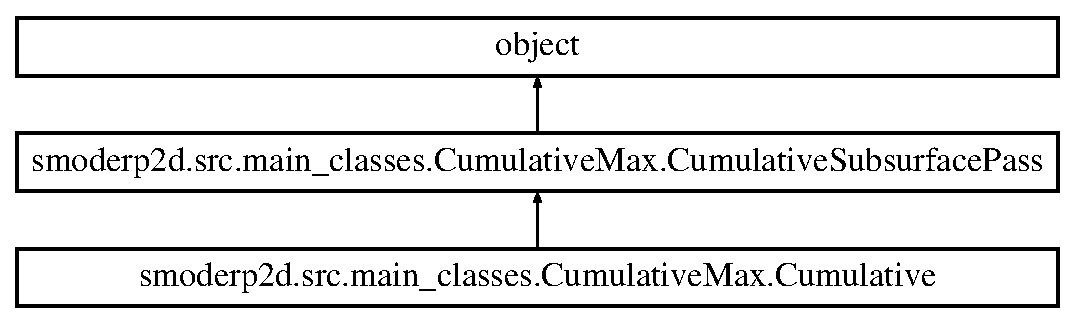
\includegraphics[height=3.000000cm]{d4/d62/classsmoderp2d_1_1src_1_1main__classes_1_1CumulativeMax_1_1CumulativeSubsurfacePass}
\end{center}
\end{figure}
\subsection*{Public Member Functions}
\begin{DoxyCompactItemize}
\item 
def \hyperlink{classsmoderp2d_1_1src_1_1main__classes_1_1CumulativeMax_1_1CumulativeSubsurfacePass_a4cd34bafce5287c9f1ca7ebcf1f941a6}{update\-\_\-cumulative\-\_\-sur}
\begin{DoxyCompactList}\small\item\em Method is used after each time step. \end{DoxyCompactList}\end{DoxyCompactItemize}


\subsection{Detailed Description}
Empty (pass) Class. 

Class is inherited by the class \hyperlink{classsmoderp2d_1_1src_1_1main__classes_1_1CumulativeMax_1_1Cumulative}{Cumulative} if the subsurface flow is not desired. 

Definition at line 111 of file Cumulative\-Max.\-py.



\subsection{Member Function Documentation}
\hypertarget{classsmoderp2d_1_1src_1_1main__classes_1_1CumulativeMax_1_1CumulativeSubsurfacePass_a4cd34bafce5287c9f1ca7ebcf1f941a6}{\index{smoderp2d\-::src\-::main\-\_\-classes\-::\-Cumulative\-Max\-::\-Cumulative\-Subsurface\-Pass@{smoderp2d\-::src\-::main\-\_\-classes\-::\-Cumulative\-Max\-::\-Cumulative\-Subsurface\-Pass}!update\-\_\-cumulative\-\_\-sur@{update\-\_\-cumulative\-\_\-sur}}
\index{update\-\_\-cumulative\-\_\-sur@{update\-\_\-cumulative\-\_\-sur}!smoderp2d::src::main_classes::CumulativeMax::CumulativeSubsurfacePass@{smoderp2d\-::src\-::main\-\_\-classes\-::\-Cumulative\-Max\-::\-Cumulative\-Subsurface\-Pass}}
\subsubsection[{update\-\_\-cumulative\-\_\-sur}]{\setlength{\rightskip}{0pt plus 5cm}def smoderp2d.\-src.\-main\-\_\-classes.\-Cumulative\-Max.\-Cumulative\-Subsurface\-Pass.\-update\-\_\-cumulative\-\_\-sur (
\begin{DoxyParamCaption}
\item[{}]{self, }
\item[{}]{i, }
\item[{}]{j, }
\item[{}]{sub, }
\item[{}]{q\-\_\-subsur}
\end{DoxyParamCaption}
)}}\label{classsmoderp2d_1_1src_1_1main__classes_1_1CumulativeMax_1_1CumulativeSubsurfacePass_a4cd34bafce5287c9f1ca7ebcf1f941a6}


Method is used after each time step. 

Method is called in \hyperlink{namespacesmoderp2d_1_1src_1_1runoff}{smoderp2d.\-src.\-runoff} 

Definition at line 117 of file Cumulative\-Max.\-py.


\begin{DoxyCode}
117 
118   \textcolor{keyword}{def }\hyperlink{classsmoderp2d_1_1src_1_1main__classes_1_1CumulativeMax_1_1CumulativeSubsurfacePass_a4cd34bafce5287c9f1ca7ebcf1f941a6}{update\_cumulative\_sur}(self,i,j,sub,q\_subsur):
119     \textcolor{keywordflow}{pass}
120 
121 
122 
123 
124 
125 
126 
127 
128 
129 

\end{DoxyCode}


The documentation for this class was generated from the following file\-:\begin{DoxyCompactItemize}
\item 
smoderp2d/src/main\-\_\-classes/Cumulative\-Max.\-py\end{DoxyCompactItemize}

\hypertarget{classsmoderp2d_1_1src_1_1main__classes_1_1Flow_1_1D8}{\section{smoderp2d.\-src.\-main\-\_\-classes.\-Flow.\-D8 Class Reference}
\label{classsmoderp2d_1_1src_1_1main__classes_1_1Flow_1_1D8}\index{smoderp2d.\-src.\-main\-\_\-classes.\-Flow.\-D8@{smoderp2d.\-src.\-main\-\_\-classes.\-Flow.\-D8}}
}


Defines methods for executing the one direction flow algorithm \hyperlink{classsmoderp2d_1_1src_1_1main__classes_1_1Flow_1_1D8}{D8}.  


Inheritance diagram for smoderp2d.\-src.\-main\-\_\-classes.\-Flow.\-D8\-:\begin{figure}[H]
\begin{center}
\leavevmode
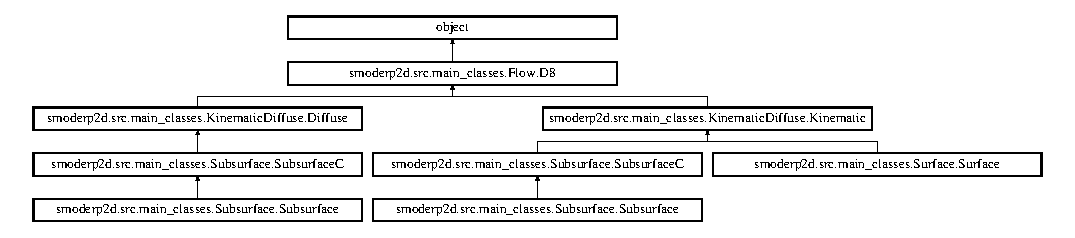
\includegraphics[height=2.753196cm]{da/d29/classsmoderp2d_1_1src_1_1main__classes_1_1Flow_1_1D8}
\end{center}
\end{figure}
\subsection*{Public Member Functions}
\begin{DoxyCompactItemize}
\item 
def \hyperlink{classsmoderp2d_1_1src_1_1main__classes_1_1Flow_1_1D8_a67744c5c6a4fe44565c0bdd52f513413}{\-\_\-\-\_\-init\-\_\-\-\_\-}
\begin{DoxyCompactList}\small\item\em constructor \end{DoxyCompactList}\item 
def \hyperlink{classsmoderp2d_1_1src_1_1main__classes_1_1Flow_1_1D8_a2c6113c6519048d1cd03869a270fad2e}{update\-\_\-inflows}
\begin{DoxyCompactList}\small\item\em updates \#inflows list if the diffuse approach is used. \end{DoxyCompactList}\item 
def \hyperlink{classsmoderp2d_1_1src_1_1main__classes_1_1Flow_1_1D8_a0a85901450ca94f202da3a609b4797eb}{cell\-\_\-runoff}
\begin{DoxyCompactList}\small\item\em returns the water volume water flows into cell i , j from the previous time step based on the \#inflows list, \par
\end{DoxyCompactList}\end{DoxyCompactItemize}
\subsection*{Public Attributes}
\begin{DoxyCompactItemize}
\item 
\hypertarget{classsmoderp2d_1_1src_1_1main__classes_1_1Flow_1_1D8_ae1e1934cd4984fc86d164b60c54788c4}{{\bfseries inflows}}\label{classsmoderp2d_1_1src_1_1main__classes_1_1Flow_1_1D8_ae1e1934cd4984fc86d164b60c54788c4}

\end{DoxyCompactItemize}


\subsection{Detailed Description}
Defines methods for executing the one direction flow algorithm \hyperlink{classsmoderp2d_1_1src_1_1main__classes_1_1Flow_1_1D8}{D8}. 

Can be inherited by the Classes\-:


\begin{DoxyItemize}
\item \hyperlink{classsmoderp2d_1_1src_1_1main__classes_1_1KinematicDiffuse_1_1Kinematic}{smoderp2d.\-src.\-main\-\_\-classes.\-Kinematic\-Diffuse.\-Kinematic}
\item \hyperlink{classsmoderp2d_1_1src_1_1main__classes_1_1KinematicDiffuse_1_1Diffuse}{smoderp2d.\-src.\-main\-\_\-classes.\-Kinematic\-Diffuse.\-Diffuse} 
\end{DoxyItemize}

Definition at line 51 of file Flow.\-py.



\subsection{Constructor \& Destructor Documentation}
\hypertarget{classsmoderp2d_1_1src_1_1main__classes_1_1Flow_1_1D8_a67744c5c6a4fe44565c0bdd52f513413}{\index{smoderp2d\-::src\-::main\-\_\-classes\-::\-Flow\-::\-D8@{smoderp2d\-::src\-::main\-\_\-classes\-::\-Flow\-::\-D8}!\-\_\-\-\_\-init\-\_\-\-\_\-@{\-\_\-\-\_\-init\-\_\-\-\_\-}}
\index{\-\_\-\-\_\-init\-\_\-\-\_\-@{\-\_\-\-\_\-init\-\_\-\-\_\-}!smoderp2d::src::main_classes::Flow::D8@{smoderp2d\-::src\-::main\-\_\-classes\-::\-Flow\-::\-D8}}
\subsubsection[{\-\_\-\-\_\-init\-\_\-\-\_\-}]{\setlength{\rightskip}{0pt plus 5cm}def smoderp2d.\-src.\-main\-\_\-classes.\-Flow.\-D8.\-\_\-\-\_\-init\-\_\-\-\_\- (
\begin{DoxyParamCaption}
\item[{}]{self}
\end{DoxyParamCaption}
)}}\label{classsmoderp2d_1_1src_1_1main__classes_1_1Flow_1_1D8_a67744c5c6a4fe44565c0bdd52f513413}


constructor 

defines inflows list which defines the flow direction for each cell of the D\-E\-M. The kinematic approach is used the inflows are defines only once in this constructor. 

Definition at line 60 of file Flow.\-py.


\begin{DoxyCode}
60 
61   \textcolor{keyword}{def }\hyperlink{classsmoderp2d_1_1src_1_1main__classes_1_1Flow_1_1D8_a67744c5c6a4fe44565c0bdd52f513413}{\_\_init\_\_}(self):
62     prt.message(\textcolor{stringliteral}{"\(\backslash\)tD8 flow algorithm"})
63     self.\hyperlink{classsmoderp2d_1_1src_1_1main__classes_1_1Flow_1_1D8_ae1e1934cd4984fc86d164b60c54788c4}{inflows} = D8\_.new\_inflows(Gl.mat\_fd)
64 
65 

\end{DoxyCode}


\subsection{Member Function Documentation}
\hypertarget{classsmoderp2d_1_1src_1_1main__classes_1_1Flow_1_1D8_a0a85901450ca94f202da3a609b4797eb}{\index{smoderp2d\-::src\-::main\-\_\-classes\-::\-Flow\-::\-D8@{smoderp2d\-::src\-::main\-\_\-classes\-::\-Flow\-::\-D8}!cell\-\_\-runoff@{cell\-\_\-runoff}}
\index{cell\-\_\-runoff@{cell\-\_\-runoff}!smoderp2d::src::main_classes::Flow::D8@{smoderp2d\-::src\-::main\-\_\-classes\-::\-Flow\-::\-D8}}
\subsubsection[{cell\-\_\-runoff}]{\setlength{\rightskip}{0pt plus 5cm}def smoderp2d.\-src.\-main\-\_\-classes.\-Flow.\-D8.\-cell\-\_\-runoff (
\begin{DoxyParamCaption}
\item[{}]{self, }
\item[{}]{i, }
\item[{}]{j}
\end{DoxyParamCaption}
)}}\label{classsmoderp2d_1_1src_1_1main__classes_1_1Flow_1_1D8_a0a85901450ca94f202da3a609b4797eb}


returns the water volume water flows into cell i , j from the previous time step based on the \#inflows list, \par


\#inflows list definition is shown in the method new\-\_\-inflows() in the package smoderp2d.\-src.\-flow\-\_\-algorithm.\-D8

The total inflow is sum of sheet and rill runoff volume.

\begin{DoxyReturn}{Returns}
inflow\-\_\-from\-\_\-cells inflow volume from the adjacent cells 
\end{DoxyReturn}


Definition at line 84 of file Flow.\-py.


\begin{DoxyCode}
84 
85   \textcolor{keyword}{def }\hyperlink{classsmoderp2d_1_1src_1_1main__classes_1_1Flow_1_1D8_a0a85901450ca94f202da3a609b4797eb}{cell\_runoff}(self,i,j):
86     inflow\_from\_cells = 0.0
87     \textcolor{keywordflow}{for} z \textcolor{keywordflow}{in} range(len(self.\hyperlink{classsmoderp2d_1_1src_1_1main__classes_1_1Flow_1_1D8_ae1e1934cd4984fc86d164b60c54788c4}{inflows}[i][j])):
88       ax = self.\hyperlink{classsmoderp2d_1_1src_1_1main__classes_1_1Flow_1_1D8_ae1e1934cd4984fc86d164b60c54788c4}{inflows}[i][j][z][0]
89       bx = self.\hyperlink{classsmoderp2d_1_1src_1_1main__classes_1_1Flow_1_1D8_ae1e1934cd4984fc86d164b60c54788c4}{inflows}[i][j][z][1]
90       iax = i+ax
91       jbx = j+bx
92       \textcolor{keywordflow}{try}:
93         insurfflow\_from\_cell = self.arr[iax][jbx].V\_runoff
94       \textcolor{keywordflow}{except}:
95         insurfflow\_from\_cell = 0.0
96       \textcolor{keywordflow}{try}:
97         inrillflow\_from\_cell = self.arr[iax][jbx].V\_runoff\_rill
98       \textcolor{keywordflow}{except}:
99         inrillflow\_from\_cell = 0.0
100       inflow\_from\_cells = inflow\_from\_cells + insurfflow\_from\_cell + inrillflow\_from\_cell
101 
102     
103 
104     \textcolor{keywordflow}{return} inflow\_from\_cells
105 
106 
107 
108 
109 
110 
111 
112 
113 
114 
115 
116 
117 
118 
119 
120 
121 
122 
123 

\end{DoxyCode}
\hypertarget{classsmoderp2d_1_1src_1_1main__classes_1_1Flow_1_1D8_a2c6113c6519048d1cd03869a270fad2e}{\index{smoderp2d\-::src\-::main\-\_\-classes\-::\-Flow\-::\-D8@{smoderp2d\-::src\-::main\-\_\-classes\-::\-Flow\-::\-D8}!update\-\_\-inflows@{update\-\_\-inflows}}
\index{update\-\_\-inflows@{update\-\_\-inflows}!smoderp2d::src::main_classes::Flow::D8@{smoderp2d\-::src\-::main\-\_\-classes\-::\-Flow\-::\-D8}}
\subsubsection[{update\-\_\-inflows}]{\setlength{\rightskip}{0pt plus 5cm}def smoderp2d.\-src.\-main\-\_\-classes.\-Flow.\-D8.\-update\-\_\-inflows (
\begin{DoxyParamCaption}
\item[{}]{self, }
\item[{}]{fd}
\end{DoxyParamCaption}
)}}\label{classsmoderp2d_1_1src_1_1main__classes_1_1Flow_1_1D8_a2c6113c6519048d1cd03869a270fad2e}


updates \#inflows list if the diffuse approach is used. 

In the diffusive approach the flow direction may change due to changes of the water level. 

Definition at line 70 of file Flow.\-py.


\begin{DoxyCode}
70 
71   \textcolor{keyword}{def }\hyperlink{classsmoderp2d_1_1src_1_1main__classes_1_1Flow_1_1D8_a2c6113c6519048d1cd03869a270fad2e}{update\_inflows}(self,fd):
72     self.\hyperlink{classsmoderp2d_1_1src_1_1main__classes_1_1Flow_1_1D8_ae1e1934cd4984fc86d164b60c54788c4}{inflows} = D8\_.new\_inflows(fd)
73 
74 

\end{DoxyCode}


The documentation for this class was generated from the following file\-:\begin{DoxyCompactItemize}
\item 
smoderp2d/src/main\-\_\-classes/Flow.\-py\end{DoxyCompactItemize}

\hypertarget{classsmoderp2d_1_1src_1_1tools_1_1tools_1_1DebugMark}{\section{smoderp2d.\-src.\-tools.\-tools.\-Debug\-Mark Class Reference}
\label{classsmoderp2d_1_1src_1_1tools_1_1tools_1_1DebugMark}\index{smoderp2d.\-src.\-tools.\-tools.\-Debug\-Mark@{smoderp2d.\-src.\-tools.\-tools.\-Debug\-Mark}}
}


Class with the debug mark.  


\subsection*{Public Member Functions}
\begin{DoxyCompactItemize}
\item 
\hypertarget{classsmoderp2d_1_1src_1_1tools_1_1tools_1_1DebugMark_a8bcee985b3cf188f578d8f7cb3ecd397}{def {\bfseries mark}}\label{classsmoderp2d_1_1src_1_1tools_1_1tools_1_1DebugMark_a8bcee985b3cf188f578d8f7cb3ecd397}

\end{DoxyCompactItemize}
\subsection*{Static Public Attributes}
\begin{DoxyCompactItemize}
\item 
\hypertarget{classsmoderp2d_1_1src_1_1tools_1_1tools_1_1DebugMark_a8b644b7480d760e4870851c64b50a2e6}{int {\bfseries n} = 0}\label{classsmoderp2d_1_1src_1_1tools_1_1tools_1_1DebugMark_a8b644b7480d760e4870851c64b50a2e6}

\end{DoxyCompactItemize}


\subsection{Detailed Description}
Class with the debug mark. 

method self.\-mark with given name return konsole message with generically increasing integer value 

Definition at line 9 of file tools.\-py.



The documentation for this class was generated from the following file\-:\begin{DoxyCompactItemize}
\item 
smoderp2d/src/tools/tools.\-py\end{DoxyCompactItemize}

\hypertarget{classsmoderp2d_1_1src_1_1main__classes_1_1KinematicDiffuse_1_1Diffuse}{\section{smoderp2d.\-src.\-main\-\_\-classes.\-Kinematic\-Diffuse.\-Diffuse Class Reference}
\label{classsmoderp2d_1_1src_1_1main__classes_1_1KinematicDiffuse_1_1Diffuse}\index{smoderp2d.\-src.\-main\-\_\-classes.\-Kinematic\-Diffuse.\-Diffuse@{smoderp2d.\-src.\-main\-\_\-classes.\-Kinematic\-Diffuse.\-Diffuse}}
}
Inheritance diagram for smoderp2d.\-src.\-main\-\_\-classes.\-Kinematic\-Diffuse.\-Diffuse\-:\begin{figure}[H]
\begin{center}
\leavevmode
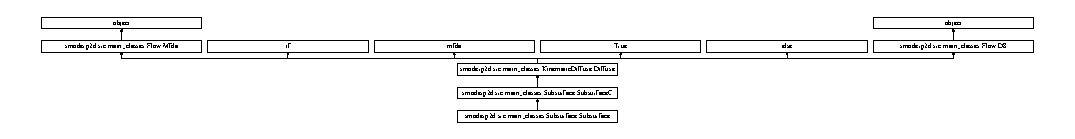
\includegraphics[height=1.414141cm]{d0/d0a/classsmoderp2d_1_1src_1_1main__classes_1_1KinematicDiffuse_1_1Diffuse}
\end{center}
\end{figure}
\subsection*{Public Member Functions}
\begin{DoxyCompactItemize}
\item 
\hypertarget{classsmoderp2d_1_1src_1_1main__classes_1_1KinematicDiffuse_1_1Diffuse_a037b417e061247ef505ca1416f65006c}{def {\bfseries \-\_\-\-\_\-init\-\_\-\-\_\-}}\label{classsmoderp2d_1_1src_1_1main__classes_1_1KinematicDiffuse_1_1Diffuse_a037b417e061247ef505ca1416f65006c}

\item 
\hypertarget{classsmoderp2d_1_1src_1_1main__classes_1_1KinematicDiffuse_1_1Diffuse_a927915b728f8e553dfd8d62733e27bf5}{def {\bfseries new\-\_\-inflows}}\label{classsmoderp2d_1_1src_1_1main__classes_1_1KinematicDiffuse_1_1Diffuse_a927915b728f8e553dfd8d62733e27bf5}

\item 
\hypertarget{classsmoderp2d_1_1src_1_1main__classes_1_1KinematicDiffuse_1_1Diffuse_a7e70d7ef597897be0d0acdfe3390ce1b}{def {\bfseries update\-\_\-\-H}}\label{classsmoderp2d_1_1src_1_1main__classes_1_1KinematicDiffuse_1_1Diffuse_a7e70d7ef597897be0d0acdfe3390ce1b}

\end{DoxyCompactItemize}
\subsection*{Public Attributes}
\begin{DoxyCompactItemize}
\item 
\hypertarget{classsmoderp2d_1_1src_1_1main__classes_1_1KinematicDiffuse_1_1Diffuse_a35cd9807eadd4db62eeafe7c657475a9}{{\bfseries H}}\label{classsmoderp2d_1_1src_1_1main__classes_1_1KinematicDiffuse_1_1Diffuse_a35cd9807eadd4db62eeafe7c657475a9}

\end{DoxyCompactItemize}


\subsection{Detailed Description}


Definition at line 42 of file Kinematic\-Diffuse.\-py.



The documentation for this class was generated from the following file\-:\begin{DoxyCompactItemize}
\item 
smoderp2d/src/main\-\_\-classes/Kinematic\-Diffuse.\-py\end{DoxyCompactItemize}

\hypertarget{classsmoderp2d_1_1src_1_1stream__functions_1_1stream__preparation_1_1Error}{\section{smoderp2d.\-src.\-stream\-\_\-functions.\-stream\-\_\-preparation.\-Error Class Reference}
\label{classsmoderp2d_1_1src_1_1stream__functions_1_1stream__preparation_1_1Error}\index{smoderp2d.\-src.\-stream\-\_\-functions.\-stream\-\_\-preparation.\-Error@{smoderp2d.\-src.\-stream\-\_\-functions.\-stream\-\_\-preparation.\-Error}}
}
Inheritance diagram for smoderp2d.\-src.\-stream\-\_\-functions.\-stream\-\_\-preparation.\-Error\-:\begin{figure}[H]
\begin{center}
\leavevmode
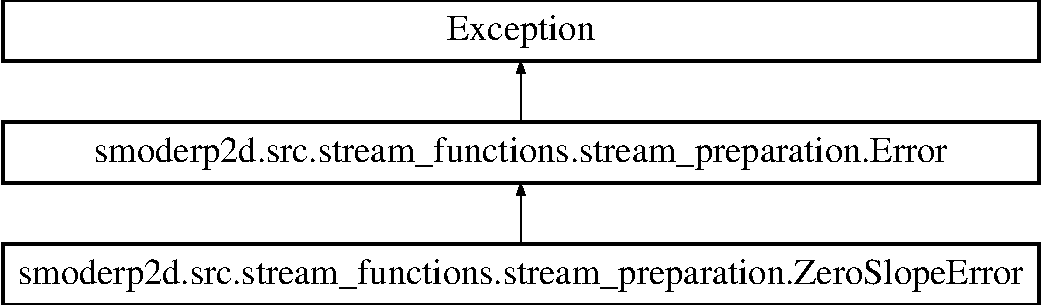
\includegraphics[height=3.000000cm]{dd/d48/classsmoderp2d_1_1src_1_1stream__functions_1_1stream__preparation_1_1Error}
\end{center}
\end{figure}


\subsection{Detailed Description}
\begin{DoxyVerb}Base class for exceptions in this module.\end{DoxyVerb}
 

Definition at line 34 of file stream\-\_\-preparation.\-py.



The documentation for this class was generated from the following file\-:\begin{DoxyCompactItemize}
\item 
smoderp2d/src/stream\-\_\-functions/stream\-\_\-preparation.\-py\end{DoxyCompactItemize}

\hypertarget{classsmoderp2d_1_1config_1_1Error}{\section{smoderp2d.\-config.\-Error Class Reference}
\label{classsmoderp2d_1_1config_1_1Error}\index{smoderp2d.\-config.\-Error@{smoderp2d.\-config.\-Error}}
}
Inheritance diagram for smoderp2d.\-config.\-Error\-:\begin{figure}[H]
\begin{center}
\leavevmode
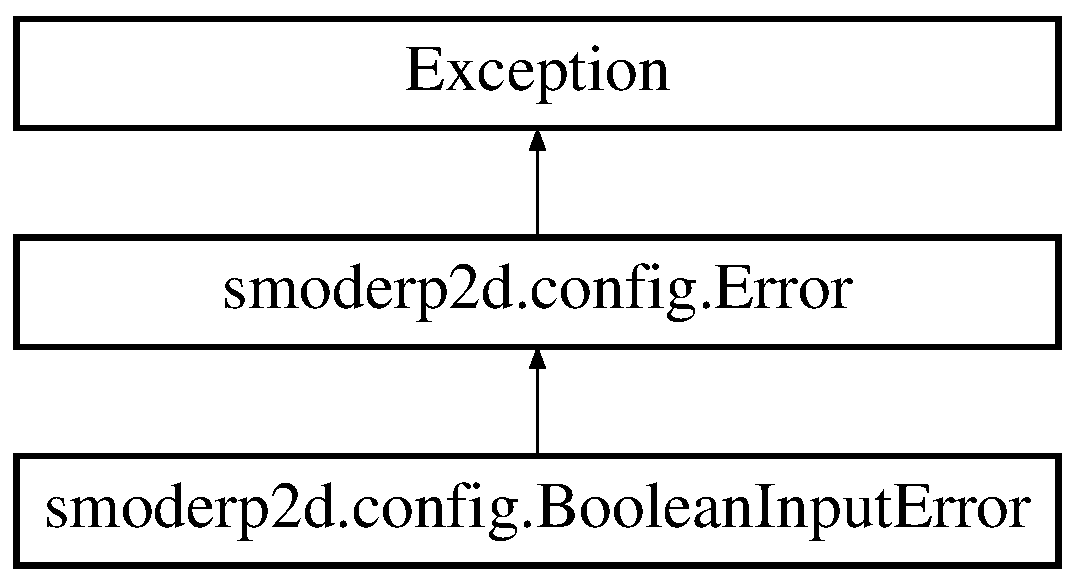
\includegraphics[height=3.000000cm]{classsmoderp2d_1_1config_1_1Error}
\end{center}
\end{figure}


\subsection{Detailed Description}
\begin{DoxyVerb}Base class for exceptions in this module.\end{DoxyVerb}
 

The documentation for this class was generated from the following file\-:\begin{DoxyCompactItemize}
\item 
smoderp2d/config.\-py\end{DoxyCompactItemize}

\hypertarget{classsmoderp2d_1_1src_1_1processes_1_1rainfall_1_1Error}{\section{smoderp2d.\-src.\-processes.\-rainfall.\-Error Class Reference}
\label{classsmoderp2d_1_1src_1_1processes_1_1rainfall_1_1Error}\index{smoderp2d.\-src.\-processes.\-rainfall.\-Error@{smoderp2d.\-src.\-processes.\-rainfall.\-Error}}
}
Inheritance diagram for smoderp2d.\-src.\-processes.\-rainfall.\-Error\-:\begin{figure}[H]
\begin{center}
\leavevmode
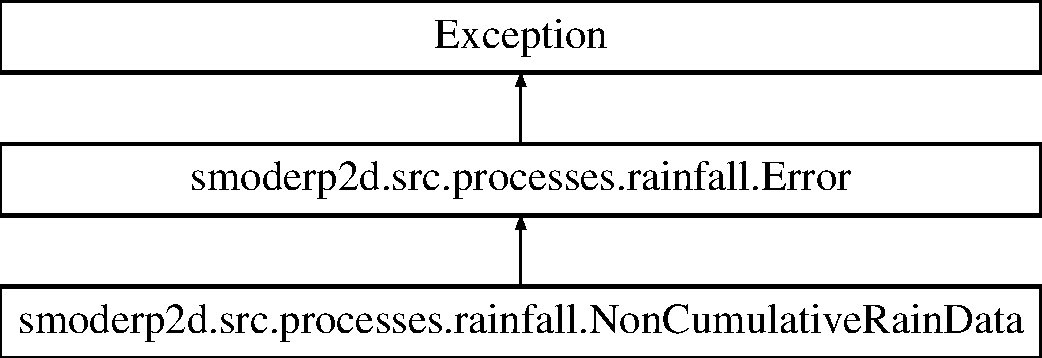
\includegraphics[height=3.000000cm]{d6/d1d/classsmoderp2d_1_1src_1_1processes_1_1rainfall_1_1Error}
\end{center}
\end{figure}


\subsection{Detailed Description}
\begin{DoxyVerb}Base class for exceptions in this module.\end{DoxyVerb}
 

Definition at line 13 of file rainfall.\-py.



The documentation for this class was generated from the following file\-:\begin{DoxyCompactItemize}
\item 
smoderp2d/src/processes/rainfall.\-py\end{DoxyCompactItemize}

\hypertarget{classsmoderp2d_1_1src_1_1tools_1_1tools_1_1FileNameGen}{\section{smoderp2d.\-src.\-tools.\-tools.\-File\-Name\-Gen Class Reference}
\label{classsmoderp2d_1_1src_1_1tools_1_1tools_1_1FileNameGen}\index{smoderp2d.\-src.\-tools.\-tools.\-File\-Name\-Gen@{smoderp2d.\-src.\-tools.\-tools.\-File\-Name\-Gen}}
}


Class with the file name generation.  


\subsection*{Public Member Functions}
\begin{DoxyCompactItemize}
\item 
\hypertarget{classsmoderp2d_1_1src_1_1tools_1_1tools_1_1FileNameGen_a643b6c519d6395cc62f74e4dcc65cbe5}{def {\bfseries \-\_\-\-\_\-init\-\_\-\-\_\-}}\label{classsmoderp2d_1_1src_1_1tools_1_1tools_1_1FileNameGen_a643b6c519d6395cc62f74e4dcc65cbe5}

\item 
\hypertarget{classsmoderp2d_1_1src_1_1tools_1_1tools_1_1FileNameGen_a6ba5778ecc01d6ab70dbe4b476ab72ca}{def {\bfseries gen}}\label{classsmoderp2d_1_1src_1_1tools_1_1tools_1_1FileNameGen_a6ba5778ecc01d6ab70dbe4b476ab72ca}

\end{DoxyCompactItemize}
\subsection*{Public Attributes}
\begin{DoxyCompactItemize}
\item 
\hypertarget{classsmoderp2d_1_1src_1_1tools_1_1tools_1_1FileNameGen_a5da7416b45adcbab881ab48df88ed49f}{{\bfseries n}}\label{classsmoderp2d_1_1src_1_1tools_1_1tools_1_1FileNameGen_a5da7416b45adcbab881ab48df88ed49f}

\end{DoxyCompactItemize}


\subsection{Detailed Description}
Class with the file name generation. 

method self.\-gen with given name returns the name plus increasing int number 000$\ast$ 

Definition at line 18 of file tools.\-py.



The documentation for this class was generated from the following file\-:\begin{DoxyCompactItemize}
\item 
smoderp2d/src/tools/tools.\-py\end{DoxyCompactItemize}

\hypertarget{classsmoderp2d_1_1src_1_1main__classes_1_1General_1_1Globals}{\section{smoderp2d.\-src.\-main\-\_\-classes.\-General.\-Globals Class Reference}
\label{classsmoderp2d_1_1src_1_1main__classes_1_1General_1_1Globals}\index{smoderp2d.\-src.\-main\-\_\-classes.\-General.\-Globals@{smoderp2d.\-src.\-main\-\_\-classes.\-General.\-Globals}}
}


Class \hyperlink{classsmoderp2d_1_1src_1_1main__classes_1_1General_1_1Globals}{Globals} contains global variables.  


Inheritance diagram for smoderp2d.\-src.\-main\-\_\-classes.\-General.\-Globals\-:\begin{figure}[H]
\begin{center}
\leavevmode
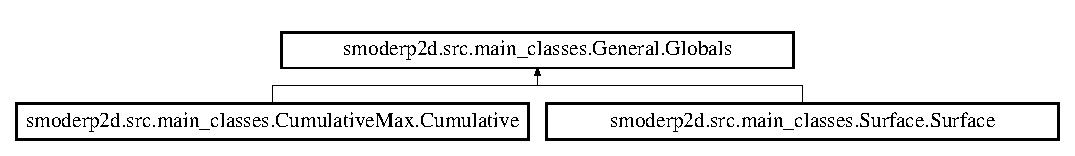
\includegraphics[height=1.651917cm]{classsmoderp2d_1_1src_1_1main__classes_1_1General_1_1Globals}
\end{center}
\end{figure}
\subsection*{Public Member Functions}
\begin{DoxyCompactItemize}
\item 
\hypertarget{classsmoderp2d_1_1src_1_1main__classes_1_1General_1_1Globals_ad3000f7a68bcd48b8e90c345f40c49d1}{def {\bfseries get\-\_\-pixel\-\_\-area}}\label{classsmoderp2d_1_1src_1_1main__classes_1_1General_1_1Globals_ad3000f7a68bcd48b8e90c345f40c49d1}

\item 
\hypertarget{classsmoderp2d_1_1src_1_1main__classes_1_1General_1_1Globals_aa5137658b7eca350872dd4dc2e170102}{def {\bfseries get\-\_\-rows}}\label{classsmoderp2d_1_1src_1_1main__classes_1_1General_1_1Globals_aa5137658b7eca350872dd4dc2e170102}

\item 
\hypertarget{classsmoderp2d_1_1src_1_1main__classes_1_1General_1_1Globals_a6cab1fdbed3e3fca488cd13e6b5ac76f}{def {\bfseries get\-\_\-cols}}\label{classsmoderp2d_1_1src_1_1main__classes_1_1General_1_1Globals_a6cab1fdbed3e3fca488cd13e6b5ac76f}

\item 
\hypertarget{classsmoderp2d_1_1src_1_1main__classes_1_1General_1_1Globals_a1bd9293607c1f722b22e162bce6ab9f0}{def {\bfseries get\-\_\-rrows}}\label{classsmoderp2d_1_1src_1_1main__classes_1_1General_1_1Globals_a1bd9293607c1f722b22e162bce6ab9f0}

\item 
\hypertarget{classsmoderp2d_1_1src_1_1main__classes_1_1General_1_1Globals_a7e8bbe8a693104aa1786084bd3a53d5c}{def {\bfseries get\-\_\-bor\-\_\-rows}}\label{classsmoderp2d_1_1src_1_1main__classes_1_1General_1_1Globals_a7e8bbe8a693104aa1786084bd3a53d5c}

\item 
\hypertarget{classsmoderp2d_1_1src_1_1main__classes_1_1General_1_1Globals_a67e67c6cf10dc651f98cf61fc0ec9321}{def {\bfseries get\-\_\-bor\-\_\-cols}}\label{classsmoderp2d_1_1src_1_1main__classes_1_1General_1_1Globals_a67e67c6cf10dc651f98cf61fc0ec9321}

\item 
\hypertarget{classsmoderp2d_1_1src_1_1main__classes_1_1General_1_1Globals_a44d24e803208ebd8718b731afb6b0701}{def {\bfseries get\-\_\-xllcorner}}\label{classsmoderp2d_1_1src_1_1main__classes_1_1General_1_1Globals_a44d24e803208ebd8718b731afb6b0701}

\item 
\hypertarget{classsmoderp2d_1_1src_1_1main__classes_1_1General_1_1Globals_a7c8046882ddec2a2dfa0c4133286eb76}{def {\bfseries get\-\_\-yllcorner}}\label{classsmoderp2d_1_1src_1_1main__classes_1_1General_1_1Globals_a7c8046882ddec2a2dfa0c4133286eb76}

\item 
\hypertarget{classsmoderp2d_1_1src_1_1main__classes_1_1General_1_1Globals_a5cb531f8c7dadd3fe69a4544993358d9}{def {\bfseries get\-\_\-\-No\-Data\-Value}}\label{classsmoderp2d_1_1src_1_1main__classes_1_1General_1_1Globals_a5cb531f8c7dadd3fe69a4544993358d9}

\item 
\hypertarget{classsmoderp2d_1_1src_1_1main__classes_1_1General_1_1Globals_a6300f1d8431feb7a390708f3420b46f7}{def {\bfseries get\-\_\-\-No\-Data\-Int}}\label{classsmoderp2d_1_1src_1_1main__classes_1_1General_1_1Globals_a6300f1d8431feb7a390708f3420b46f7}

\item 
\hypertarget{classsmoderp2d_1_1src_1_1main__classes_1_1General_1_1Globals_a70a1bb9b56f7442677ed06408eb611f3}{def {\bfseries get\-\_\-dx}}\label{classsmoderp2d_1_1src_1_1main__classes_1_1General_1_1Globals_a70a1bb9b56f7442677ed06408eb611f3}

\item 
\hypertarget{classsmoderp2d_1_1src_1_1main__classes_1_1General_1_1Globals_aef442883e5888787f54c62e6f0b50b50}{def {\bfseries get\-\_\-dy}}\label{classsmoderp2d_1_1src_1_1main__classes_1_1General_1_1Globals_aef442883e5888787f54c62e6f0b50b50}

\item 
\hypertarget{classsmoderp2d_1_1src_1_1main__classes_1_1General_1_1Globals_a9c4ee3d23a1ae64b9f445a2deb651cb2}{def {\bfseries get\-\_\-type\-\_\-of\-\_\-computing}}\label{classsmoderp2d_1_1src_1_1main__classes_1_1General_1_1Globals_a9c4ee3d23a1ae64b9f445a2deb651cb2}

\item 
\hypertarget{classsmoderp2d_1_1src_1_1main__classes_1_1General_1_1Globals_a21b62249ae3f62f38848e675384bba05}{def {\bfseries get\-\_\-outdir}}\label{classsmoderp2d_1_1src_1_1main__classes_1_1General_1_1Globals_a21b62249ae3f62f38848e675384bba05}

\item 
\hypertarget{classsmoderp2d_1_1src_1_1main__classes_1_1General_1_1Globals_a0a5befa9f8cebf1d5674c87a10add88e}{def {\bfseries get\-\_\-mat\-\_\-boundary}}\label{classsmoderp2d_1_1src_1_1main__classes_1_1General_1_1Globals_a0a5befa9f8cebf1d5674c87a10add88e}

\item 
\hypertarget{classsmoderp2d_1_1src_1_1main__classes_1_1General_1_1Globals_adf666d9dcd64d5f9d1489a925319f764}{def {\bfseries get\-\_\-outlet\-Cells}}\label{classsmoderp2d_1_1src_1_1main__classes_1_1General_1_1Globals_adf666d9dcd64d5f9d1489a925319f764}

\item 
\hypertarget{classsmoderp2d_1_1src_1_1main__classes_1_1General_1_1Globals_a5df7deb5ba08735568a7d0abf81e0e1a}{def {\bfseries get\-\_\-array\-\_\-points}}\label{classsmoderp2d_1_1src_1_1main__classes_1_1General_1_1Globals_a5df7deb5ba08735568a7d0abf81e0e1a}

\item 
\hypertarget{classsmoderp2d_1_1src_1_1main__classes_1_1General_1_1Globals_a8bf1dad82bc18b9a25a4cb980056f9f0}{def {\bfseries get\-\_\-combinat\-Index}}\label{classsmoderp2d_1_1src_1_1main__classes_1_1General_1_1Globals_a8bf1dad82bc18b9a25a4cb980056f9f0}

\item 
\hypertarget{classsmoderp2d_1_1src_1_1main__classes_1_1General_1_1Globals_a59db7f8ed5bd4ee9a64e703900b03e22}{def {\bfseries get\-\_\-delta\-\_\-t}}\label{classsmoderp2d_1_1src_1_1main__classes_1_1General_1_1Globals_a59db7f8ed5bd4ee9a64e703900b03e22}

\item 
\hypertarget{classsmoderp2d_1_1src_1_1main__classes_1_1General_1_1Globals_a0eae61fdce71c7545e4d5ac66b029f8f}{def {\bfseries get\-\_\-mat\-\_\-pi}}\label{classsmoderp2d_1_1src_1_1main__classes_1_1General_1_1Globals_a0eae61fdce71c7545e4d5ac66b029f8f}

\item 
\hypertarget{classsmoderp2d_1_1src_1_1main__classes_1_1General_1_1Globals_a54e80b99d968a1857e4cf397a4d6f797}{def {\bfseries get\-\_\-mat\-\_\-ppl}}\label{classsmoderp2d_1_1src_1_1main__classes_1_1General_1_1Globals_a54e80b99d968a1857e4cf397a4d6f797}

\item 
\hypertarget{classsmoderp2d_1_1src_1_1main__classes_1_1General_1_1Globals_ac182cc96e274bd24f4f88e713e57d317}{def {\bfseries get\-\_\-surface\-\_\-retention}}\label{classsmoderp2d_1_1src_1_1main__classes_1_1General_1_1Globals_ac182cc96e274bd24f4f88e713e57d317}

\item 
\hypertarget{classsmoderp2d_1_1src_1_1main__classes_1_1General_1_1Globals_a465f59d1a477adf218ec250badae3902}{def {\bfseries get\-\_\-mat\-\_\-inf\-\_\-index}}\label{classsmoderp2d_1_1src_1_1main__classes_1_1General_1_1Globals_a465f59d1a477adf218ec250badae3902}

\item 
\hypertarget{classsmoderp2d_1_1src_1_1main__classes_1_1General_1_1Globals_a3acb3559113d2bac1ad44abfc45ecf86}{def {\bfseries get\-\_\-mat\-\_\-hcrit}}\label{classsmoderp2d_1_1src_1_1main__classes_1_1General_1_1Globals_a3acb3559113d2bac1ad44abfc45ecf86}

\item 
\hypertarget{classsmoderp2d_1_1src_1_1main__classes_1_1General_1_1Globals_ad69b77eaf57de4fba7ef46df8b7d7ee7}{def {\bfseries get\-\_\-mat\-\_\-aa}}\label{classsmoderp2d_1_1src_1_1main__classes_1_1General_1_1Globals_ad69b77eaf57de4fba7ef46df8b7d7ee7}

\item 
\hypertarget{classsmoderp2d_1_1src_1_1main__classes_1_1General_1_1Globals_ab0ecf20324035c6cd3f2c209d5e8df18}{def {\bfseries get\-\_\-mat\-\_\-b}}\label{classsmoderp2d_1_1src_1_1main__classes_1_1General_1_1Globals_ab0ecf20324035c6cd3f2c209d5e8df18}

\item 
\hypertarget{classsmoderp2d_1_1src_1_1main__classes_1_1General_1_1Globals_a94171a7137c429e6d557842bd5287c38}{def {\bfseries get\-\_\-mat\-\_\-reten}}\label{classsmoderp2d_1_1src_1_1main__classes_1_1General_1_1Globals_a94171a7137c429e6d557842bd5287c38}

\item 
\hypertarget{classsmoderp2d_1_1src_1_1main__classes_1_1General_1_1Globals_ad581e62c5253d5334447756b2830cff7}{def {\bfseries get\-\_\-mat\-\_\-fd}}\label{classsmoderp2d_1_1src_1_1main__classes_1_1General_1_1Globals_ad581e62c5253d5334447756b2830cff7}

\item 
\hypertarget{classsmoderp2d_1_1src_1_1main__classes_1_1General_1_1Globals_a825d94c44158c58726270fd0ecf136f4}{def {\bfseries get\-\_\-mat\-\_\-dmt}}\label{classsmoderp2d_1_1src_1_1main__classes_1_1General_1_1Globals_a825d94c44158c58726270fd0ecf136f4}

\item 
\hypertarget{classsmoderp2d_1_1src_1_1main__classes_1_1General_1_1Globals_a2dba0bd2372a9b996c2ab710f2e6c082}{def {\bfseries get\-\_\-mat\-\_\-efect\-\_\-vrst}}\label{classsmoderp2d_1_1src_1_1main__classes_1_1General_1_1Globals_a2dba0bd2372a9b996c2ab710f2e6c082}

\item 
\hypertarget{classsmoderp2d_1_1src_1_1main__classes_1_1General_1_1Globals_ab7a97e5217223f9086ce069a95866ed4}{def {\bfseries get\-\_\-mat\-\_\-slope}}\label{classsmoderp2d_1_1src_1_1main__classes_1_1General_1_1Globals_ab7a97e5217223f9086ce069a95866ed4}

\item 
\hypertarget{classsmoderp2d_1_1src_1_1main__classes_1_1General_1_1Globals_ade30ebeed6461163acb5a3a2d003b5d0}{def {\bfseries get\-\_\-mat\-\_\-nan}}\label{classsmoderp2d_1_1src_1_1main__classes_1_1General_1_1Globals_ade30ebeed6461163acb5a3a2d003b5d0}

\item 
\hypertarget{classsmoderp2d_1_1src_1_1main__classes_1_1General_1_1Globals_ae66b16d2dd4ddf898230e928d3a41eda}{def {\bfseries get\-\_\-mat\-\_\-a}}\label{classsmoderp2d_1_1src_1_1main__classes_1_1General_1_1Globals_ae66b16d2dd4ddf898230e928d3a41eda}

\item 
\hypertarget{classsmoderp2d_1_1src_1_1main__classes_1_1General_1_1Globals_a6f4b227477f02eced43dbf1125d8277b}{def {\bfseries get\-\_\-mat\-\_\-n}}\label{classsmoderp2d_1_1src_1_1main__classes_1_1General_1_1Globals_a6f4b227477f02eced43dbf1125d8277b}

\item 
\hypertarget{classsmoderp2d_1_1src_1_1main__classes_1_1General_1_1Globals_ae9879516010ae1d24d0e388905eef084}{def {\bfseries get\-\_\-points}}\label{classsmoderp2d_1_1src_1_1main__classes_1_1General_1_1Globals_ae9879516010ae1d24d0e388905eef084}

\item 
\hypertarget{classsmoderp2d_1_1src_1_1main__classes_1_1General_1_1Globals_a03ec62f07f787c8c75bd898c77276afc}{def {\bfseries get\-\_\-poradi}}\label{classsmoderp2d_1_1src_1_1main__classes_1_1General_1_1Globals_a03ec62f07f787c8c75bd898c77276afc}

\item 
\hypertarget{classsmoderp2d_1_1src_1_1main__classes_1_1General_1_1Globals_a2cb408a6cc6a41a2861b871af1be5c04}{def {\bfseries get\-\_\-end\-\_\-tim}}\label{classsmoderp2d_1_1src_1_1main__classes_1_1General_1_1Globals_a2cb408a6cc6a41a2861b871af1be5c04}

\item 
\hypertarget{classsmoderp2d_1_1src_1_1main__classes_1_1General_1_1Globals_ad822eadd746cdcb23cfd7e99cd3d591b}{def {\bfseries get\-\_\-spix}}\label{classsmoderp2d_1_1src_1_1main__classes_1_1General_1_1Globals_ad822eadd746cdcb23cfd7e99cd3d591b}

\item 
\hypertarget{classsmoderp2d_1_1src_1_1main__classes_1_1General_1_1Globals_a3643034346aeded9ee5198df7a6054a2}{def {\bfseries get\-\_\-state\-\_\-cell}}\label{classsmoderp2d_1_1src_1_1main__classes_1_1General_1_1Globals_a3643034346aeded9ee5198df7a6054a2}

\item 
\hypertarget{classsmoderp2d_1_1src_1_1main__classes_1_1General_1_1Globals_a9e956c882d0362ff8b332fdbcc478df1}{def {\bfseries get\-\_\-temp}}\label{classsmoderp2d_1_1src_1_1main__classes_1_1General_1_1Globals_a9e956c882d0362ff8b332fdbcc478df1}

\item 
\hypertarget{classsmoderp2d_1_1src_1_1main__classes_1_1General_1_1Globals_a7fe80648e65c2c6be108e350447c3cbd}{def {\bfseries get\-\_\-vpix}}\label{classsmoderp2d_1_1src_1_1main__classes_1_1General_1_1Globals_a7fe80648e65c2c6be108e350447c3cbd}

\item 
\hypertarget{classsmoderp2d_1_1src_1_1main__classes_1_1General_1_1Globals_aa12eadd3ec000198ad5c1fbe5709ccee}{def {\bfseries get\-\_\-mfda}}\label{classsmoderp2d_1_1src_1_1main__classes_1_1General_1_1Globals_aa12eadd3ec000198ad5c1fbe5709ccee}

\item 
\hypertarget{classsmoderp2d_1_1src_1_1main__classes_1_1General_1_1Globals_aaae0af638559ad6a431fcd53981d3231}{def {\bfseries get\-\_\-sr}}\label{classsmoderp2d_1_1src_1_1main__classes_1_1General_1_1Globals_aaae0af638559ad6a431fcd53981d3231}

\item 
\hypertarget{classsmoderp2d_1_1src_1_1main__classes_1_1General_1_1Globals_a1ef86073130b9dc7bb7db3ecdfe5ffb5}{def {\bfseries get\-\_\-itera}}\label{classsmoderp2d_1_1src_1_1main__classes_1_1General_1_1Globals_a1ef86073130b9dc7bb7db3ecdfe5ffb5}

\item 
\hypertarget{classsmoderp2d_1_1src_1_1main__classes_1_1General_1_1Globals_a4aaadf0fd2d0c88fa860ec4118d60839}{def {\bfseries get\-\_\-toky}}\label{classsmoderp2d_1_1src_1_1main__classes_1_1General_1_1Globals_a4aaadf0fd2d0c88fa860ec4118d60839}

\item 
\hypertarget{classsmoderp2d_1_1src_1_1main__classes_1_1General_1_1Globals_ac4ecf46bc4c0134e07b6eea373b20e88}{def {\bfseries get\-\_\-cell\-\_\-stream}}\label{classsmoderp2d_1_1src_1_1main__classes_1_1General_1_1Globals_ac4ecf46bc4c0134e07b6eea373b20e88}

\item 
\hypertarget{classsmoderp2d_1_1src_1_1main__classes_1_1General_1_1Globals_a02cd6195c2cda0819f2b855611667100}{def {\bfseries get\-\_\-mat\-\_\-tok\-\_\-usek}}\label{classsmoderp2d_1_1src_1_1main__classes_1_1General_1_1Globals_a02cd6195c2cda0819f2b855611667100}

\item 
\hypertarget{classsmoderp2d_1_1src_1_1main__classes_1_1General_1_1Globals_ab183cbe4c6b5b3ac1b4c9b1d65180ef2}{def {\bfseries get\-\_\-\-S\-T\-R\-E\-A\-M\-\_\-\-R\-A\-T\-I\-O}}\label{classsmoderp2d_1_1src_1_1main__classes_1_1General_1_1Globals_ab183cbe4c6b5b3ac1b4c9b1d65180ef2}

\item 
\hypertarget{classsmoderp2d_1_1src_1_1main__classes_1_1General_1_1Globals_aeeced572deac2a2bbaa9890fae510247}{def {\bfseries get\-\_\-toky\-Loc}}\label{classsmoderp2d_1_1src_1_1main__classes_1_1General_1_1Globals_aeeced572deac2a2bbaa9890fae510247}

\end{DoxyCompactItemize}
\subsection*{Static Public Attributes}
\begin{DoxyCompactItemize}
\item 
\hypertarget{classsmoderp2d_1_1src_1_1main__classes_1_1General_1_1Globals_a3d946a5e9e780d8da49b612367587d70}{\hyperlink{classsmoderp2d_1_1src_1_1main__classes_1_1General_1_1Globals_a3d946a5e9e780d8da49b612367587d70}{pixel\-\_\-area} = None}\label{classsmoderp2d_1_1src_1_1main__classes_1_1General_1_1Globals_a3d946a5e9e780d8da49b612367587d70}

\begin{DoxyCompactList}\small\item\em area of a raster cell in meters \end{DoxyCompactList}\item 
\hypertarget{classsmoderp2d_1_1src_1_1main__classes_1_1General_1_1Globals_a69f9371306b49a71b87726b9142ea866}{\hyperlink{classsmoderp2d_1_1src_1_1main__classes_1_1General_1_1Globals_a69f9371306b49a71b87726b9142ea866}{r} = None}\label{classsmoderp2d_1_1src_1_1main__classes_1_1General_1_1Globals_a69f9371306b49a71b87726b9142ea866}

\begin{DoxyCompactList}\small\item\em number of rows in rasters \end{DoxyCompactList}\item 
\hypertarget{classsmoderp2d_1_1src_1_1main__classes_1_1General_1_1Globals_afe9be194e183190e467e005fd8817a64}{\hyperlink{classsmoderp2d_1_1src_1_1main__classes_1_1General_1_1Globals_afe9be194e183190e467e005fd8817a64}{c} = None}\label{classsmoderp2d_1_1src_1_1main__classes_1_1General_1_1Globals_afe9be194e183190e467e005fd8817a64}

\begin{DoxyCompactList}\small\item\em number of columns in rasters \end{DoxyCompactList}\item 
\hypertarget{classsmoderp2d_1_1src_1_1main__classes_1_1General_1_1Globals_a46f72d33658564beee5f50c9b7509f20}{\hyperlink{classsmoderp2d_1_1src_1_1main__classes_1_1General_1_1Globals_a46f72d33658564beee5f50c9b7509f20}{rr} = None}\label{classsmoderp2d_1_1src_1_1main__classes_1_1General_1_1Globals_a46f72d33658564beee5f50c9b7509f20}

\begin{DoxyCompactList}\small\item\em id of rows in computational domain \end{DoxyCompactList}\item 
\hypertarget{classsmoderp2d_1_1src_1_1main__classes_1_1General_1_1Globals_a54e48c95dfb31da8eb7a1232449197d4}{\hyperlink{classsmoderp2d_1_1src_1_1main__classes_1_1General_1_1Globals_a54e48c95dfb31da8eb7a1232449197d4}{rc} = None}\label{classsmoderp2d_1_1src_1_1main__classes_1_1General_1_1Globals_a54e48c95dfb31da8eb7a1232449197d4}

\begin{DoxyCompactList}\small\item\em id of columns in computational domain \end{DoxyCompactList}\item 
\hypertarget{classsmoderp2d_1_1src_1_1main__classes_1_1General_1_1Globals_a0611140edd6cbc2770b34dfe64417939}{\hyperlink{classsmoderp2d_1_1src_1_1main__classes_1_1General_1_1Globals_a0611140edd6cbc2770b34dfe64417939}{br} = None}\label{classsmoderp2d_1_1src_1_1main__classes_1_1General_1_1Globals_a0611140edd6cbc2770b34dfe64417939}

\begin{DoxyCompactList}\small\item\em id of rows in at the boundary of computational domain \end{DoxyCompactList}\item 
\hypertarget{classsmoderp2d_1_1src_1_1main__classes_1_1General_1_1Globals_ae727c98eef401d052789cfcbd636ca0b}{\hyperlink{classsmoderp2d_1_1src_1_1main__classes_1_1General_1_1Globals_ae727c98eef401d052789cfcbd636ca0b}{bc} = None}\label{classsmoderp2d_1_1src_1_1main__classes_1_1General_1_1Globals_ae727c98eef401d052789cfcbd636ca0b}

\begin{DoxyCompactList}\small\item\em id of columns in at the boundary of computational domain \end{DoxyCompactList}\item 
\hypertarget{classsmoderp2d_1_1src_1_1main__classes_1_1General_1_1Globals_ae1284ec1dde185ed719dd5a3f47b6a23}{\hyperlink{classsmoderp2d_1_1src_1_1main__classes_1_1General_1_1Globals_ae1284ec1dde185ed719dd5a3f47b6a23}{xllcorner} = None}\label{classsmoderp2d_1_1src_1_1main__classes_1_1General_1_1Globals_ae1284ec1dde185ed719dd5a3f47b6a23}

\begin{DoxyCompactList}\small\item\em x coordinate od of left bottom corner of raster \end{DoxyCompactList}\item 
\hypertarget{classsmoderp2d_1_1src_1_1main__classes_1_1General_1_1Globals_af131760c403479b939a11904eb65b3c0}{\hyperlink{classsmoderp2d_1_1src_1_1main__classes_1_1General_1_1Globals_af131760c403479b939a11904eb65b3c0}{yllcorner} = None}\label{classsmoderp2d_1_1src_1_1main__classes_1_1General_1_1Globals_af131760c403479b939a11904eb65b3c0}

\begin{DoxyCompactList}\small\item\em y coordinate od of left bottom corner of raster \end{DoxyCompactList}\item 
\hypertarget{classsmoderp2d_1_1src_1_1main__classes_1_1General_1_1Globals_ab5d999609842e6a6b5c344286e370931}{\hyperlink{classsmoderp2d_1_1src_1_1main__classes_1_1General_1_1Globals_ab5d999609842e6a6b5c344286e370931}{No\-Data\-Value} = None}\label{classsmoderp2d_1_1src_1_1main__classes_1_1General_1_1Globals_ab5d999609842e6a6b5c344286e370931}

\begin{DoxyCompactList}\small\item\em no data value for raster \end{DoxyCompactList}\item 
\hypertarget{classsmoderp2d_1_1src_1_1main__classes_1_1General_1_1Globals_ae94f95b04165905eec5c2830a5cea14b}{\hyperlink{classsmoderp2d_1_1src_1_1main__classes_1_1General_1_1Globals_ae94f95b04165905eec5c2830a5cea14b}{No\-Data\-Int} = None}\label{classsmoderp2d_1_1src_1_1main__classes_1_1General_1_1Globals_ae94f95b04165905eec5c2830a5cea14b}

\begin{DoxyCompactList}\small\item\em no data integer value for raster \end{DoxyCompactList}\item 
\hypertarget{classsmoderp2d_1_1src_1_1main__classes_1_1General_1_1Globals_af0476c5752e99031490082dde8036ca7}{\hyperlink{classsmoderp2d_1_1src_1_1main__classes_1_1General_1_1Globals_af0476c5752e99031490082dde8036ca7}{dx} = None}\label{classsmoderp2d_1_1src_1_1main__classes_1_1General_1_1Globals_af0476c5752e99031490082dde8036ca7}

\begin{DoxyCompactList}\small\item\em size of raster cell \end{DoxyCompactList}\item 
\hypertarget{classsmoderp2d_1_1src_1_1main__classes_1_1General_1_1Globals_a467231ff30ce69dd31ea6abf28aad9eb}{\hyperlink{classsmoderp2d_1_1src_1_1main__classes_1_1General_1_1Globals_a467231ff30ce69dd31ea6abf28aad9eb}{dy} = None}\label{classsmoderp2d_1_1src_1_1main__classes_1_1General_1_1Globals_a467231ff30ce69dd31ea6abf28aad9eb}

\begin{DoxyCompactList}\small\item\em size of raster cell \end{DoxyCompactList}\item 
\hypertarget{classsmoderp2d_1_1src_1_1main__classes_1_1General_1_1Globals_a44829cc45efe34502c40508be44f74c4}{\hyperlink{classsmoderp2d_1_1src_1_1main__classes_1_1General_1_1Globals_a44829cc45efe34502c40508be44f74c4}{type\-\_\-of\-\_\-computing} = None}\label{classsmoderp2d_1_1src_1_1main__classes_1_1General_1_1Globals_a44829cc45efe34502c40508be44f74c4}

\begin{DoxyCompactList}\small\item\em type of computation \end{DoxyCompactList}\item 
\hypertarget{classsmoderp2d_1_1src_1_1main__classes_1_1General_1_1Globals_ae67bcaa2f0c00799126d060052aaec83}{\hyperlink{classsmoderp2d_1_1src_1_1main__classes_1_1General_1_1Globals_ae67bcaa2f0c00799126d060052aaec83}{outdir} = None}\label{classsmoderp2d_1_1src_1_1main__classes_1_1General_1_1Globals_ae67bcaa2f0c00799126d060052aaec83}

\begin{DoxyCompactList}\small\item\em path to a output directory \end{DoxyCompactList}\item 
\hypertarget{classsmoderp2d_1_1src_1_1main__classes_1_1General_1_1Globals_a9402ef35548d4b8bf964c0cb992f1a33}{\hyperlink{classsmoderp2d_1_1src_1_1main__classes_1_1General_1_1Globals_a9402ef35548d4b8bf964c0cb992f1a33}{mat\-\_\-boundary} = None}\label{classsmoderp2d_1_1src_1_1main__classes_1_1General_1_1Globals_a9402ef35548d4b8bf964c0cb992f1a33}

\begin{DoxyCompactList}\small\item\em raster with labeled boundary cells \end{DoxyCompactList}\item 
\hypertarget{classsmoderp2d_1_1src_1_1main__classes_1_1General_1_1Globals_a94f8a60495282029b7ececab5480abc8}{\hyperlink{classsmoderp2d_1_1src_1_1main__classes_1_1General_1_1Globals_a94f8a60495282029b7ececab5480abc8}{outlet\-Cells} = None}\label{classsmoderp2d_1_1src_1_1main__classes_1_1General_1_1Globals_a94f8a60495282029b7ececab5480abc8}

\begin{DoxyCompactList}\small\item\em list containing coordinates of catchment outlet cells \end{DoxyCompactList}\item 
\hypertarget{classsmoderp2d_1_1src_1_1main__classes_1_1General_1_1Globals_a559814dc0182fb454d556f65ceb11fb2}{\hyperlink{classsmoderp2d_1_1src_1_1main__classes_1_1General_1_1Globals_a559814dc0182fb454d556f65ceb11fb2}{array\-\_\-points} = None}\label{classsmoderp2d_1_1src_1_1main__classes_1_1General_1_1Globals_a559814dc0182fb454d556f65ceb11fb2}

\begin{DoxyCompactList}\small\item\em array containing information of hydrogram points \end{DoxyCompactList}\item 
\hypertarget{classsmoderp2d_1_1src_1_1main__classes_1_1General_1_1Globals_a2b7b70ababe7d68b5b5b532d9f33eab4}{\hyperlink{classsmoderp2d_1_1src_1_1main__classes_1_1General_1_1Globals_a2b7b70ababe7d68b5b5b532d9f33eab4}{combinat\-Index} = None}\label{classsmoderp2d_1_1src_1_1main__classes_1_1General_1_1Globals_a2b7b70ababe7d68b5b5b532d9f33eab4}

\begin{DoxyCompactList}\small\item\em combinat\-Index \end{DoxyCompactList}\item 
\hypertarget{classsmoderp2d_1_1src_1_1main__classes_1_1General_1_1Globals_af75f48fb9adca164f8d669fb2d0e40a3}{\hyperlink{classsmoderp2d_1_1src_1_1main__classes_1_1General_1_1Globals_af75f48fb9adca164f8d669fb2d0e40a3}{delta\-\_\-t} = None}\label{classsmoderp2d_1_1src_1_1main__classes_1_1General_1_1Globals_af75f48fb9adca164f8d669fb2d0e40a3}

\begin{DoxyCompactList}\small\item\em time step \end{DoxyCompactList}\item 
\hypertarget{classsmoderp2d_1_1src_1_1main__classes_1_1General_1_1Globals_a9e124cfe8415a1815e57184c771828c9}{\hyperlink{classsmoderp2d_1_1src_1_1main__classes_1_1General_1_1Globals_a9e124cfe8415a1815e57184c771828c9}{mat\-\_\-pi} = None}\label{classsmoderp2d_1_1src_1_1main__classes_1_1General_1_1Globals_a9e124cfe8415a1815e57184c771828c9}

\begin{DoxyCompactList}\small\item\em raster contains potential interception data \end{DoxyCompactList}\item 
\hypertarget{classsmoderp2d_1_1src_1_1main__classes_1_1General_1_1Globals_a1922e8e8e5ad59475630c04f9563cb0e}{\hyperlink{classsmoderp2d_1_1src_1_1main__classes_1_1General_1_1Globals_a1922e8e8e5ad59475630c04f9563cb0e}{mat\-\_\-ppl} = None}\label{classsmoderp2d_1_1src_1_1main__classes_1_1General_1_1Globals_a1922e8e8e5ad59475630c04f9563cb0e}

\begin{DoxyCompactList}\small\item\em raster contains leaf area data \end{DoxyCompactList}\item 
\hypertarget{classsmoderp2d_1_1src_1_1main__classes_1_1General_1_1Globals_a0086b0ddb2e910b265cc0b3f35a4f6b9}{\hyperlink{classsmoderp2d_1_1src_1_1main__classes_1_1General_1_1Globals_a0086b0ddb2e910b265cc0b3f35a4f6b9}{surface\-\_\-retention} = None}\label{classsmoderp2d_1_1src_1_1main__classes_1_1General_1_1Globals_a0086b0ddb2e910b265cc0b3f35a4f6b9}

\begin{DoxyCompactList}\small\item\em raster contains surface retention data \end{DoxyCompactList}\item 
\hypertarget{classsmoderp2d_1_1src_1_1main__classes_1_1General_1_1Globals_a632d6fa7a167fa90e1846beba9ab6d54}{\hyperlink{classsmoderp2d_1_1src_1_1main__classes_1_1General_1_1Globals_a632d6fa7a167fa90e1846beba9ab6d54}{mat\-\_\-inf\-\_\-index} = None}\label{classsmoderp2d_1_1src_1_1main__classes_1_1General_1_1Globals_a632d6fa7a167fa90e1846beba9ab6d54}

\begin{DoxyCompactList}\small\item\em raster contains id of infiltration type \end{DoxyCompactList}\item 
\hypertarget{classsmoderp2d_1_1src_1_1main__classes_1_1General_1_1Globals_affb07f2f32920313ce60f10fd2f80877}{\hyperlink{classsmoderp2d_1_1src_1_1main__classes_1_1General_1_1Globals_affb07f2f32920313ce60f10fd2f80877}{mat\-\_\-hcrit} = None}\label{classsmoderp2d_1_1src_1_1main__classes_1_1General_1_1Globals_affb07f2f32920313ce60f10fd2f80877}

\begin{DoxyCompactList}\small\item\em raster contains critical water level \end{DoxyCompactList}\item 
\hypertarget{classsmoderp2d_1_1src_1_1main__classes_1_1General_1_1Globals_a5e404bdda3ded4c57a7c5a55c0fcee8b}{\hyperlink{classsmoderp2d_1_1src_1_1main__classes_1_1General_1_1Globals_a5e404bdda3ded4c57a7c5a55c0fcee8b}{mat\-\_\-aa} = None}\label{classsmoderp2d_1_1src_1_1main__classes_1_1General_1_1Globals_a5e404bdda3ded4c57a7c5a55c0fcee8b}

\begin{DoxyCompactList}\small\item\em raster contains parameter of power law for surface runoff \end{DoxyCompactList}\item 
\hypertarget{classsmoderp2d_1_1src_1_1main__classes_1_1General_1_1Globals_a0c7ba0b3f75bc4798db722985957c42f}{\hyperlink{classsmoderp2d_1_1src_1_1main__classes_1_1General_1_1Globals_a0c7ba0b3f75bc4798db722985957c42f}{mat\-\_\-b} = None}\label{classsmoderp2d_1_1src_1_1main__classes_1_1General_1_1Globals_a0c7ba0b3f75bc4798db722985957c42f}

\begin{DoxyCompactList}\small\item\em raster contains parameter of power law for surface runoff \end{DoxyCompactList}\item 
\hypertarget{classsmoderp2d_1_1src_1_1main__classes_1_1General_1_1Globals_a123c03ff4576b88c14f49e3f9cbdc668}{\hyperlink{classsmoderp2d_1_1src_1_1main__classes_1_1General_1_1Globals_a123c03ff4576b88c14f49e3f9cbdc668}{mat\-\_\-reten} = None}\label{classsmoderp2d_1_1src_1_1main__classes_1_1General_1_1Globals_a123c03ff4576b88c14f49e3f9cbdc668}

\begin{DoxyCompactList}\small\item\em raster contains surface retention data \end{DoxyCompactList}\item 
\hypertarget{classsmoderp2d_1_1src_1_1main__classes_1_1General_1_1Globals_afbce795e06901216c2161a6dccb30b61}{\hyperlink{classsmoderp2d_1_1src_1_1main__classes_1_1General_1_1Globals_afbce795e06901216c2161a6dccb30b61}{mat\-\_\-fd} = None}\label{classsmoderp2d_1_1src_1_1main__classes_1_1General_1_1Globals_afbce795e06901216c2161a6dccb30b61}

\begin{DoxyCompactList}\small\item\em raster contains flow direction datas \end{DoxyCompactList}\item 
\hypertarget{classsmoderp2d_1_1src_1_1main__classes_1_1General_1_1Globals_aa761f096bf400a98909a771e38126748}{\hyperlink{classsmoderp2d_1_1src_1_1main__classes_1_1General_1_1Globals_aa761f096bf400a98909a771e38126748}{mat\-\_\-dmt} = None}\label{classsmoderp2d_1_1src_1_1main__classes_1_1General_1_1Globals_aa761f096bf400a98909a771e38126748}

\begin{DoxyCompactList}\small\item\em raster contains digital elevation model \end{DoxyCompactList}\item 
\hypertarget{classsmoderp2d_1_1src_1_1main__classes_1_1General_1_1Globals_abd8dd7857d52c54eedbffa13053bfd5d}{\hyperlink{classsmoderp2d_1_1src_1_1main__classes_1_1General_1_1Globals_abd8dd7857d52c54eedbffa13053bfd5d}{mat\-\_\-efect\-\_\-vrst} = None}\label{classsmoderp2d_1_1src_1_1main__classes_1_1General_1_1Globals_abd8dd7857d52c54eedbffa13053bfd5d}

\begin{DoxyCompactList}\small\item\em raster contains efective couterline data \end{DoxyCompactList}\item 
\hypertarget{classsmoderp2d_1_1src_1_1main__classes_1_1General_1_1Globals_af0391ef5dc132f91e5d53af203cf2006}{\hyperlink{classsmoderp2d_1_1src_1_1main__classes_1_1General_1_1Globals_af0391ef5dc132f91e5d53af203cf2006}{mat\-\_\-slope} = None}\label{classsmoderp2d_1_1src_1_1main__classes_1_1General_1_1Globals_af0391ef5dc132f91e5d53af203cf2006}

\begin{DoxyCompactList}\small\item\em raster contains surface slopes data \end{DoxyCompactList}\item 
\hypertarget{classsmoderp2d_1_1src_1_1main__classes_1_1General_1_1Globals_a37995f3c75f6c9bb92ea4b56cea7ef78}{\hyperlink{classsmoderp2d_1_1src_1_1main__classes_1_1General_1_1Globals_a37995f3c75f6c9bb92ea4b56cea7ef78}{mat\-\_\-nan} = None}\label{classsmoderp2d_1_1src_1_1main__classes_1_1General_1_1Globals_a37995f3c75f6c9bb92ea4b56cea7ef78}

\begin{DoxyCompactList}\small\item\em raster labels not a number cells \end{DoxyCompactList}\item 
\hyperlink{classsmoderp2d_1_1src_1_1main__classes_1_1General_1_1Globals_a68216400ee957d32802e316cf9d21d75}{mat\-\_\-a} = None
\begin{DoxyCompactList}\small\item\em raster contains parameters ... \end{DoxyCompactList}\item 
\hyperlink{classsmoderp2d_1_1src_1_1main__classes_1_1General_1_1Globals_a5e657e5a7569cc4bcb1be595e5a16278}{mat\-\_\-n} = None
\begin{DoxyCompactList}\small\item\em raster contains parameters ... \end{DoxyCompactList}\item 
\hypertarget{classsmoderp2d_1_1src_1_1main__classes_1_1General_1_1Globals_a63dd4da88840264d4b8de4dcf188c728}{\hyperlink{classsmoderp2d_1_1src_1_1main__classes_1_1General_1_1Globals_a63dd4da88840264d4b8de4dcf188c728}{points} = None}\label{classsmoderp2d_1_1src_1_1main__classes_1_1General_1_1Globals_a63dd4da88840264d4b8de4dcf188c728}

\begin{DoxyCompactList}\small\item\em ??? \end{DoxyCompactList}\item 
\hypertarget{classsmoderp2d_1_1src_1_1main__classes_1_1General_1_1Globals_a8cfcdbe6cd8c5584256fe43938b2f1d9}{\hyperlink{classsmoderp2d_1_1src_1_1main__classes_1_1General_1_1Globals_a8cfcdbe6cd8c5584256fe43938b2f1d9}{poradi} = None}\label{classsmoderp2d_1_1src_1_1main__classes_1_1General_1_1Globals_a8cfcdbe6cd8c5584256fe43938b2f1d9}

\begin{DoxyCompactList}\small\item\em ??? \end{DoxyCompactList}\item 
\hypertarget{classsmoderp2d_1_1src_1_1main__classes_1_1General_1_1Globals_a4aef8ee15db910953c2d26b074076eb4}{\hyperlink{classsmoderp2d_1_1src_1_1main__classes_1_1General_1_1Globals_a4aef8ee15db910953c2d26b074076eb4}{end\-\_\-time} = None}\label{classsmoderp2d_1_1src_1_1main__classes_1_1General_1_1Globals_a4aef8ee15db910953c2d26b074076eb4}

\begin{DoxyCompactList}\small\item\em end time of computation \end{DoxyCompactList}\item 
\hypertarget{classsmoderp2d_1_1src_1_1main__classes_1_1General_1_1Globals_a8bc5be9f7e5f697ab293d63da8223666}{\hyperlink{classsmoderp2d_1_1src_1_1main__classes_1_1General_1_1Globals_a8bc5be9f7e5f697ab293d63da8223666}{spix} = None}\label{classsmoderp2d_1_1src_1_1main__classes_1_1General_1_1Globals_a8bc5be9f7e5f697ab293d63da8223666}

\begin{DoxyCompactList}\small\item\em ??? \end{DoxyCompactList}\item 
\hypertarget{classsmoderp2d_1_1src_1_1main__classes_1_1General_1_1Globals_a7a2be25b78671ca44312c24a09e2fed7}{\hyperlink{classsmoderp2d_1_1src_1_1main__classes_1_1General_1_1Globals_a7a2be25b78671ca44312c24a09e2fed7}{state\-\_\-cell} = None}\label{classsmoderp2d_1_1src_1_1main__classes_1_1General_1_1Globals_a7a2be25b78671ca44312c24a09e2fed7}

\begin{DoxyCompactList}\small\item\em raster contains cell flow state information \end{DoxyCompactList}\item 
\hypertarget{classsmoderp2d_1_1src_1_1main__classes_1_1General_1_1Globals_a8aa45c649b19e89922d48a9c5ab9dea0}{\hyperlink{classsmoderp2d_1_1src_1_1main__classes_1_1General_1_1Globals_a8aa45c649b19e89922d48a9c5ab9dea0}{temp} = None}\label{classsmoderp2d_1_1src_1_1main__classes_1_1General_1_1Globals_a8aa45c649b19e89922d48a9c5ab9dea0}

\begin{DoxyCompactList}\small\item\em path to directory for temporal data storage \end{DoxyCompactList}\item 
\hypertarget{classsmoderp2d_1_1src_1_1main__classes_1_1General_1_1Globals_a78846120813792f6692b21fe2cbd1c8d}{\hyperlink{classsmoderp2d_1_1src_1_1main__classes_1_1General_1_1Globals_a78846120813792f6692b21fe2cbd1c8d}{vpix} = None}\label{classsmoderp2d_1_1src_1_1main__classes_1_1General_1_1Globals_a78846120813792f6692b21fe2cbd1c8d}

\begin{DoxyCompactList}\small\item\em ??? \end{DoxyCompactList}\item 
\hypertarget{classsmoderp2d_1_1src_1_1main__classes_1_1General_1_1Globals_a1b742b3412586f9d996d8d3fb0f3f0d6}{\hyperlink{classsmoderp2d_1_1src_1_1main__classes_1_1General_1_1Globals_a1b742b3412586f9d996d8d3fb0f3f0d6}{mfda} = None}\label{classsmoderp2d_1_1src_1_1main__classes_1_1General_1_1Globals_a1b742b3412586f9d996d8d3fb0f3f0d6}

\begin{DoxyCompactList}\small\item\em bool variable for flow direction algorithm (false=one direction, true multiple flow direction) \end{DoxyCompactList}\item 
\hypertarget{classsmoderp2d_1_1src_1_1main__classes_1_1General_1_1Globals_a3e0e20f9176af85d6f922f170d235ec2}{\hyperlink{classsmoderp2d_1_1src_1_1main__classes_1_1General_1_1Globals_a3e0e20f9176af85d6f922f170d235ec2}{sr} = None}\label{classsmoderp2d_1_1src_1_1main__classes_1_1General_1_1Globals_a3e0e20f9176af85d6f922f170d235ec2}

\begin{DoxyCompactList}\small\item\em list contains the precipitation data \end{DoxyCompactList}\item 
\hypertarget{classsmoderp2d_1_1src_1_1main__classes_1_1General_1_1Globals_a7cc33c7a609bbfacacf886070ac076ff}{\hyperlink{classsmoderp2d_1_1src_1_1main__classes_1_1General_1_1Globals_a7cc33c7a609bbfacacf886070ac076ff}{itera} = None}\label{classsmoderp2d_1_1src_1_1main__classes_1_1General_1_1Globals_a7cc33c7a609bbfacacf886070ac076ff}

\begin{DoxyCompactList}\small\item\em counter of precipitation intervals \end{DoxyCompactList}\item 
\hypertarget{classsmoderp2d_1_1src_1_1main__classes_1_1General_1_1Globals_a939f71c7e4d61c99e6be02bbae931879}{\hyperlink{classsmoderp2d_1_1src_1_1main__classes_1_1General_1_1Globals_a939f71c7e4d61c99e6be02bbae931879}{toky} = None}\label{classsmoderp2d_1_1src_1_1main__classes_1_1General_1_1Globals_a939f71c7e4d61c99e6be02bbae931879}

\begin{DoxyCompactList}\small\item\em ??? \end{DoxyCompactList}\item 
\hypertarget{classsmoderp2d_1_1src_1_1main__classes_1_1General_1_1Globals_a529c1fe1f33e4b2bb4de2ae60f90ee8c}{\hyperlink{classsmoderp2d_1_1src_1_1main__classes_1_1General_1_1Globals_a529c1fe1f33e4b2bb4de2ae60f90ee8c}{cell\-\_\-stream} = None}\label{classsmoderp2d_1_1src_1_1main__classes_1_1General_1_1Globals_a529c1fe1f33e4b2bb4de2ae60f90ee8c}

\begin{DoxyCompactList}\small\item\em ??? \end{DoxyCompactList}\item 
\hypertarget{classsmoderp2d_1_1src_1_1main__classes_1_1General_1_1Globals_a0268885de5c8dea73da3a5803a907c1c}{\hyperlink{classsmoderp2d_1_1src_1_1main__classes_1_1General_1_1Globals_a0268885de5c8dea73da3a5803a907c1c}{mat\-\_\-tok\-\_\-usek} = None}\label{classsmoderp2d_1_1src_1_1main__classes_1_1General_1_1Globals_a0268885de5c8dea73da3a5803a907c1c}

\begin{DoxyCompactList}\small\item\em raster contains the reach id data \end{DoxyCompactList}\item 
\hypertarget{classsmoderp2d_1_1src_1_1main__classes_1_1General_1_1Globals_aba766256b0b8e97ca03f048d4f23e5b2}{\hyperlink{classsmoderp2d_1_1src_1_1main__classes_1_1General_1_1Globals_aba766256b0b8e97ca03f048d4f23e5b2}{S\-T\-R\-E\-A\-M\-\_\-\-R\-A\-T\-I\-O} = None}\label{classsmoderp2d_1_1src_1_1main__classes_1_1General_1_1Globals_aba766256b0b8e97ca03f048d4f23e5b2}

\begin{DoxyCompactList}\small\item\em ??? \end{DoxyCompactList}\item 
\hypertarget{classsmoderp2d_1_1src_1_1main__classes_1_1General_1_1Globals_adc1192d1698e2859edc055965c14b783}{\hyperlink{classsmoderp2d_1_1src_1_1main__classes_1_1General_1_1Globals_adc1192d1698e2859edc055965c14b783}{toky\-Loc} = None}\label{classsmoderp2d_1_1src_1_1main__classes_1_1General_1_1Globals_adc1192d1698e2859edc055965c14b783}

\begin{DoxyCompactList}\small\item\em ??? \end{DoxyCompactList}\end{DoxyCompactItemize}


\subsection{Detailed Description}
Class \hyperlink{classsmoderp2d_1_1src_1_1main__classes_1_1General_1_1Globals}{Globals} contains global variables. 

from \hyperlink{namespacesmoderp2d_1_1src_1_1data__preparation}{data\-\_\-preparation}, in instance of class needed the data are taken from import of this class 

\subsection{Member Data Documentation}
\hypertarget{classsmoderp2d_1_1src_1_1main__classes_1_1General_1_1Globals_a68216400ee957d32802e316cf9d21d75}{\index{smoderp2d\-::src\-::main\-\_\-classes\-::\-General\-::\-Globals@{smoderp2d\-::src\-::main\-\_\-classes\-::\-General\-::\-Globals}!mat\-\_\-a@{mat\-\_\-a}}
\index{mat\-\_\-a@{mat\-\_\-a}!smoderp2d::src::main_classes::General::Globals@{smoderp2d\-::src\-::main\-\_\-classes\-::\-General\-::\-Globals}}
\subsubsection[{mat\-\_\-a}]{\setlength{\rightskip}{0pt plus 5cm}smoderp2d.\-src.\-main\-\_\-classes.\-General.\-Globals.\-mat\-\_\-a = None\hspace{0.3cm}{\ttfamily [static]}}}\label{classsmoderp2d_1_1src_1_1main__classes_1_1General_1_1Globals_a68216400ee957d32802e316cf9d21d75}


raster contains parameters ... 

\hypertarget{classsmoderp2d_1_1src_1_1main__classes_1_1General_1_1Globals_a5e657e5a7569cc4bcb1be595e5a16278}{\index{smoderp2d\-::src\-::main\-\_\-classes\-::\-General\-::\-Globals@{smoderp2d\-::src\-::main\-\_\-classes\-::\-General\-::\-Globals}!mat\-\_\-n@{mat\-\_\-n}}
\index{mat\-\_\-n@{mat\-\_\-n}!smoderp2d::src::main_classes::General::Globals@{smoderp2d\-::src\-::main\-\_\-classes\-::\-General\-::\-Globals}}
\subsubsection[{mat\-\_\-n}]{\setlength{\rightskip}{0pt plus 5cm}smoderp2d.\-src.\-main\-\_\-classes.\-General.\-Globals.\-mat\-\_\-n = None\hspace{0.3cm}{\ttfamily [static]}}}\label{classsmoderp2d_1_1src_1_1main__classes_1_1General_1_1Globals_a5e657e5a7569cc4bcb1be595e5a16278}


raster contains parameters ... 



The documentation for this class was generated from the following file\-:\begin{DoxyCompactItemize}
\item 
smoderp2d/src/main\-\_\-classes/General.\-py\end{DoxyCompactItemize}

\hypertarget{classsmoderp2d_1_1src_1_1io__functions_1_1hydrographs_1_1Hydrographs}{\section{smoderp2d.\-src.\-io\-\_\-functions.\-hydrographs.\-Hydrographs Class Reference}
\label{classsmoderp2d_1_1src_1_1io__functions_1_1hydrographs_1_1Hydrographs}\index{smoderp2d.\-src.\-io\-\_\-functions.\-hydrographs.\-Hydrographs@{smoderp2d.\-src.\-io\-\_\-functions.\-hydrographs.\-Hydrographs}}
}
\subsection*{Public Member Functions}
\begin{DoxyCompactItemize}
\item 
\hypertarget{classsmoderp2d_1_1src_1_1io__functions_1_1hydrographs_1_1Hydrographs_acc52f4f6bb0d17c422ce78fa266c6b2d}{def {\bfseries \-\_\-\-\_\-init\-\_\-\-\_\-}}\label{classsmoderp2d_1_1src_1_1io__functions_1_1hydrographs_1_1Hydrographs_acc52f4f6bb0d17c422ce78fa266c6b2d}

\item 
\hypertarget{classsmoderp2d_1_1src_1_1io__functions_1_1hydrographs_1_1Hydrographs_a29819629062100b2f045751a1a5e7bf1}{def {\bfseries write\-\_\-hydrographs\-\_\-record}}\label{classsmoderp2d_1_1src_1_1io__functions_1_1hydrographs_1_1Hydrographs_a29819629062100b2f045751a1a5e7bf1}

\item 
\hypertarget{classsmoderp2d_1_1src_1_1io__functions_1_1hydrographs_1_1Hydrographs_aea319aedbe9588c46fb1a7d8b6216423}{def {\bfseries close\-Hydrographs}}\label{classsmoderp2d_1_1src_1_1io__functions_1_1hydrographs_1_1Hydrographs_aea319aedbe9588c46fb1a7d8b6216423}

\end{DoxyCompactItemize}
\subsection*{Public Attributes}
\begin{DoxyCompactItemize}
\item 
\hypertarget{classsmoderp2d_1_1src_1_1io__functions_1_1hydrographs_1_1Hydrographs_a4c5e3ad9606b153d5c56002ca2b3899d}{{\bfseries in\-Surface}}\label{classsmoderp2d_1_1src_1_1io__functions_1_1hydrographs_1_1Hydrographs_a4c5e3ad9606b153d5c56002ca2b3899d}

\item 
\hypertarget{classsmoderp2d_1_1src_1_1io__functions_1_1hydrographs_1_1Hydrographs_a4642e344d4fe5b318889deee9499f2bd}{{\bfseries in\-Stream}}\label{classsmoderp2d_1_1src_1_1io__functions_1_1hydrographs_1_1Hydrographs_a4642e344d4fe5b318889deee9499f2bd}

\item 
\hypertarget{classsmoderp2d_1_1src_1_1io__functions_1_1hydrographs_1_1Hydrographs_a4c96a2a9e8a0370e1225194d1498943f}{{\bfseries n}}\label{classsmoderp2d_1_1src_1_1io__functions_1_1hydrographs_1_1Hydrographs_a4c96a2a9e8a0370e1225194d1498943f}

\item 
\hypertarget{classsmoderp2d_1_1src_1_1io__functions_1_1hydrographs_1_1Hydrographs_ad2422ef3c027b57ee515a1b9428f578d}{{\bfseries point\-\_\-int}}\label{classsmoderp2d_1_1src_1_1io__functions_1_1hydrographs_1_1Hydrographs_ad2422ef3c027b57ee515a1b9428f578d}

\item 
\hypertarget{classsmoderp2d_1_1src_1_1io__functions_1_1hydrographs_1_1Hydrographs_a1d17eb088af27bfaa0c3efc2390c7ce7}{{\bfseries subflow}}\label{classsmoderp2d_1_1src_1_1io__functions_1_1hydrographs_1_1Hydrographs_a1d17eb088af27bfaa0c3efc2390c7ce7}

\item 
\hypertarget{classsmoderp2d_1_1src_1_1io__functions_1_1hydrographs_1_1Hydrographs_a7d1bb8d892cf07cfe7a99c9770f15166}{{\bfseries rill}}\label{classsmoderp2d_1_1src_1_1io__functions_1_1hydrographs_1_1Hydrographs_a7d1bb8d892cf07cfe7a99c9770f15166}

\item 
\hypertarget{classsmoderp2d_1_1src_1_1io__functions_1_1hydrographs_1_1Hydrographs_a409d0269b91717abb0863d679b4f7368}{{\bfseries stream}}\label{classsmoderp2d_1_1src_1_1io__functions_1_1hydrographs_1_1Hydrographs_a409d0269b91717abb0863d679b4f7368}

\item 
\hypertarget{classsmoderp2d_1_1src_1_1io__functions_1_1hydrographs_1_1Hydrographs_a2ba88b55e9014ae1591c0d687b429248}{{\bfseries pixel\-\_\-area}}\label{classsmoderp2d_1_1src_1_1io__functions_1_1hydrographs_1_1Hydrographs_a2ba88b55e9014ae1591c0d687b429248}

\item 
\hypertarget{classsmoderp2d_1_1src_1_1io__functions_1_1hydrographs_1_1Hydrographs_a699682863e80d885651ab31f68949e0d}{{\bfseries header}}\label{classsmoderp2d_1_1src_1_1io__functions_1_1hydrographs_1_1Hydrographs_a699682863e80d885651ab31f68949e0d}

\item 
\hypertarget{classsmoderp2d_1_1src_1_1io__functions_1_1hydrographs_1_1Hydrographs_a656de4c1982efe371c36388bef0ec844}{{\bfseries files}}\label{classsmoderp2d_1_1src_1_1io__functions_1_1hydrographs_1_1Hydrographs_a656de4c1982efe371c36388bef0ec844}

\end{DoxyCompactItemize}


\subsection{Detailed Description}


Definition at line 13 of file hydrographs.\-py.



The documentation for this class was generated from the following file\-:\begin{DoxyCompactItemize}
\item 
smoderp2d/src/io\-\_\-functions/hydrographs.\-py\end{DoxyCompactItemize}

\hypertarget{classsmoderp2d_1_1src_1_1io__functions_1_1hydrographs_1_1HydrographsPass}{\section{smoderp2d.\-src.\-io\-\_\-functions.\-hydrographs.\-Hydrographs\-Pass Class Reference}
\label{classsmoderp2d_1_1src_1_1io__functions_1_1hydrographs_1_1HydrographsPass}\index{smoderp2d.\-src.\-io\-\_\-functions.\-hydrographs.\-Hydrographs\-Pass@{smoderp2d.\-src.\-io\-\_\-functions.\-hydrographs.\-Hydrographs\-Pass}}
}
\subsection*{Public Member Functions}
\begin{DoxyCompactItemize}
\item 
\hypertarget{classsmoderp2d_1_1src_1_1io__functions_1_1hydrographs_1_1HydrographsPass_a76fee1fd128fa9c9d26fede127fc68b7}{def {\bfseries write\-\_\-hydrographs\-\_\-record}}\label{classsmoderp2d_1_1src_1_1io__functions_1_1hydrographs_1_1HydrographsPass_a76fee1fd128fa9c9d26fede127fc68b7}

\item 
\hypertarget{classsmoderp2d_1_1src_1_1io__functions_1_1hydrographs_1_1HydrographsPass_a8dc82a5cbcfa1d913f73004befa159e9}{def {\bfseries close\-Hydrographs}}\label{classsmoderp2d_1_1src_1_1io__functions_1_1hydrographs_1_1HydrographsPass_a8dc82a5cbcfa1d913f73004befa159e9}

\end{DoxyCompactItemize}


The documentation for this class was generated from the following file\-:\begin{DoxyCompactItemize}
\item 
smoderp2d/src/io\-\_\-functions/hydrographs.\-py\end{DoxyCompactItemize}

\hypertarget{classsmoderp2d_1_1src_1_1main__classes_1_1KinematicDiffuse_1_1Kinematic}{\section{smoderp2d.\-src.\-main\-\_\-classes.\-Kinematic\-Diffuse.\-Kinematic Class Reference}
\label{classsmoderp2d_1_1src_1_1main__classes_1_1KinematicDiffuse_1_1Kinematic}\index{smoderp2d.\-src.\-main\-\_\-classes.\-Kinematic\-Diffuse.\-Kinematic@{smoderp2d.\-src.\-main\-\_\-classes.\-Kinematic\-Diffuse.\-Kinematic}}
}
Inheritance diagram for smoderp2d.\-src.\-main\-\_\-classes.\-Kinematic\-Diffuse.\-Kinematic\-:\begin{figure}[H]
\begin{center}
\leavevmode
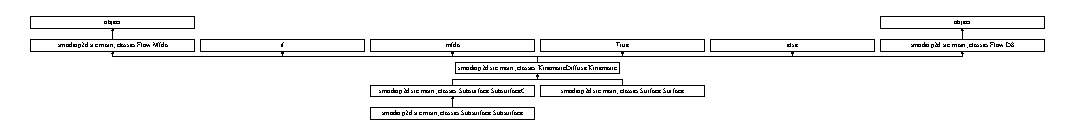
\includegraphics[height=1.376598cm]{d8/dbb/classsmoderp2d_1_1src_1_1main__classes_1_1KinematicDiffuse_1_1Kinematic}
\end{center}
\end{figure}
\subsection*{Public Member Functions}
\begin{DoxyCompactItemize}
\item 
\hypertarget{classsmoderp2d_1_1src_1_1main__classes_1_1KinematicDiffuse_1_1Kinematic_adc69a0521f7fd79c536c029d5a1d92aa}{def {\bfseries \-\_\-\-\_\-init\-\_\-\-\_\-}}\label{classsmoderp2d_1_1src_1_1main__classes_1_1KinematicDiffuse_1_1Kinematic_adc69a0521f7fd79c536c029d5a1d92aa}

\item 
\hypertarget{classsmoderp2d_1_1src_1_1main__classes_1_1KinematicDiffuse_1_1Kinematic_a1f9263e8cccf589dc954a3223730befe}{def {\bfseries new\-\_\-inflows}}\label{classsmoderp2d_1_1src_1_1main__classes_1_1KinematicDiffuse_1_1Kinematic_a1f9263e8cccf589dc954a3223730befe}

\item 
\hypertarget{classsmoderp2d_1_1src_1_1main__classes_1_1KinematicDiffuse_1_1Kinematic_aa64ce31fcbf34b0cfce9905dc7c8d8fb}{def {\bfseries update\-\_\-\-H}}\label{classsmoderp2d_1_1src_1_1main__classes_1_1KinematicDiffuse_1_1Kinematic_aa64ce31fcbf34b0cfce9905dc7c8d8fb}

\end{DoxyCompactItemize}
\subsection*{Additional Inherited Members}


\subsection{Detailed Description}


Definition at line 16 of file Kinematic\-Diffuse.\-py.



The documentation for this class was generated from the following file\-:\begin{DoxyCompactItemize}
\item 
smoderp2d/src/main\-\_\-classes/Kinematic\-Diffuse.\-py\end{DoxyCompactItemize}

\hypertarget{classsmoderp2d_1_1src_1_1tools_1_1save__load__data__nopickle_1_1LoadItems}{\section{smoderp2d.\-src.\-tools.\-save\-\_\-load\-\_\-data\-\_\-nopickle.\-Load\-Items Class Reference}
\label{classsmoderp2d_1_1src_1_1tools_1_1save__load__data__nopickle_1_1LoadItems}\index{smoderp2d.\-src.\-tools.\-save\-\_\-load\-\_\-data\-\_\-nopickle.\-Load\-Items@{smoderp2d.\-src.\-tools.\-save\-\_\-load\-\_\-data\-\_\-nopickle.\-Load\-Items}}
}


Class to load item of different typy.  


Inheritance diagram for smoderp2d.\-src.\-tools.\-save\-\_\-load\-\_\-data\-\_\-nopickle.\-Load\-Items\-:\begin{figure}[H]
\begin{center}
\leavevmode
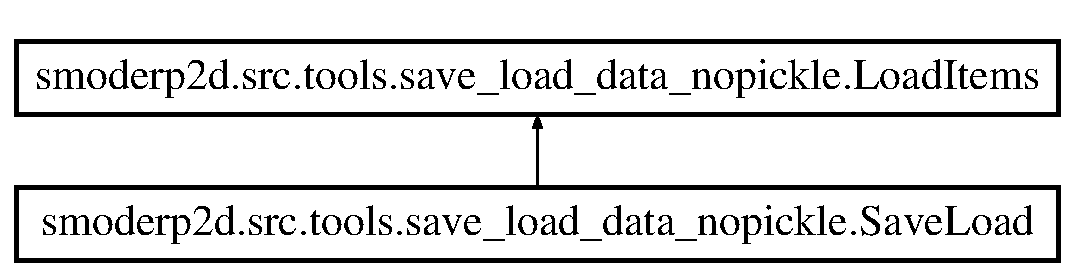
\includegraphics[height=2.000000cm]{d3/d1f/classsmoderp2d_1_1src_1_1tools_1_1save__load__data__nopickle_1_1LoadItems}
\end{center}
\end{figure}
\subsection*{Public Member Functions}
\begin{DoxyCompactItemize}
\item 
\hypertarget{classsmoderp2d_1_1src_1_1tools_1_1save__load__data__nopickle_1_1LoadItems_a0f3570e9e8bd76a954e60bde857861a7}{def {\bfseries loadlist}}\label{classsmoderp2d_1_1src_1_1tools_1_1save__load__data__nopickle_1_1LoadItems_a0f3570e9e8bd76a954e60bde857861a7}

\item 
\hypertarget{classsmoderp2d_1_1src_1_1tools_1_1save__load__data__nopickle_1_1LoadItems_a7250d369739d4a8c4bfaa7b70e4bd534}{def {\bfseries loadint}}\label{classsmoderp2d_1_1src_1_1tools_1_1save__load__data__nopickle_1_1LoadItems_a7250d369739d4a8c4bfaa7b70e4bd534}

\item 
\hypertarget{classsmoderp2d_1_1src_1_1tools_1_1save__load__data__nopickle_1_1LoadItems_a040a5d67126261103412e0a3f57e3f3a}{def {\bfseries loadfloat}}\label{classsmoderp2d_1_1src_1_1tools_1_1save__load__data__nopickle_1_1LoadItems_a040a5d67126261103412e0a3f57e3f3a}

\item 
\hypertarget{classsmoderp2d_1_1src_1_1tools_1_1save__load__data__nopickle_1_1LoadItems_a9af5877bd8f5667aedc72d4a33ca1db9}{def {\bfseries loadstr}}\label{classsmoderp2d_1_1src_1_1tools_1_1save__load__data__nopickle_1_1LoadItems_a9af5877bd8f5667aedc72d4a33ca1db9}

\item 
\hypertarget{classsmoderp2d_1_1src_1_1tools_1_1save__load__data__nopickle_1_1LoadItems_a91e3e85f8757186800d690a0e99aea0b}{def {\bfseries loadunicode}}\label{classsmoderp2d_1_1src_1_1tools_1_1save__load__data__nopickle_1_1LoadItems_a91e3e85f8757186800d690a0e99aea0b}

\item 
\hypertarget{classsmoderp2d_1_1src_1_1tools_1_1save__load__data__nopickle_1_1LoadItems_af60d09591089c53a03aa1e427055ffc0}{def {\bfseries loadnpy}}\label{classsmoderp2d_1_1src_1_1tools_1_1save__load__data__nopickle_1_1LoadItems_af60d09591089c53a03aa1e427055ffc0}

\end{DoxyCompactItemize}
\subsection*{Public Attributes}
\begin{DoxyCompactItemize}
\item 
\hypertarget{classsmoderp2d_1_1src_1_1tools_1_1save__load__data__nopickle_1_1LoadItems_a6040f17ef701cee845a742b55eb00731}{{\bfseries el}}\label{classsmoderp2d_1_1src_1_1tools_1_1save__load__data__nopickle_1_1LoadItems_a6040f17ef701cee845a742b55eb00731}

\item 
\hypertarget{classsmoderp2d_1_1src_1_1tools_1_1save__load__data__nopickle_1_1LoadItems_ac4d2dd0def0a15b24ceedbbcefba9664}{{\bfseries npyel}}\label{classsmoderp2d_1_1src_1_1tools_1_1save__load__data__nopickle_1_1LoadItems_ac4d2dd0def0a15b24ceedbbcefba9664}

\end{DoxyCompactItemize}


\subsection{Detailed Description}
Class to load item of different typy. 

Definition at line 78 of file save\-\_\-load\-\_\-data\-\_\-nopickle.\-py.



The documentation for this class was generated from the following file\-:\begin{DoxyCompactItemize}
\item 
smoderp2d/src/tools/save\-\_\-load\-\_\-data\-\_\-nopickle.\-py\end{DoxyCompactItemize}

\hypertarget{classsmoderp2d_1_1src_1_1main__classes_1_1Flow_1_1Mfda}{\section{smoderp2d.\-src.\-main\-\_\-classes.\-Flow.\-Mfda Class Reference}
\label{classsmoderp2d_1_1src_1_1main__classes_1_1Flow_1_1Mfda}\index{smoderp2d.\-src.\-main\-\_\-classes.\-Flow.\-Mfda@{smoderp2d.\-src.\-main\-\_\-classes.\-Flow.\-Mfda}}
}


Defines methods for executing the multiple flow direction algorithm mfda.  


Inheritance diagram for smoderp2d.\-src.\-main\-\_\-classes.\-Flow.\-Mfda\-:\begin{figure}[H]
\begin{center}
\leavevmode
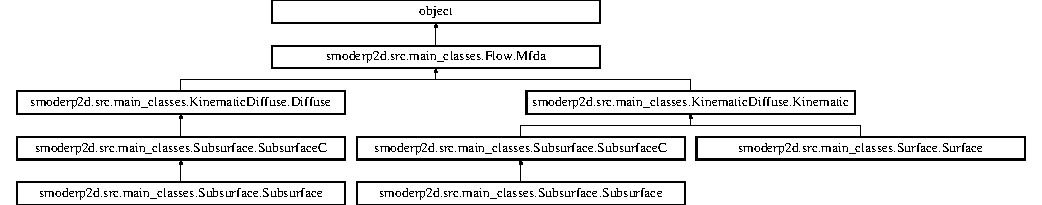
\includegraphics[height=2.753196cm]{d0/df4/classsmoderp2d_1_1src_1_1main__classes_1_1Flow_1_1Mfda}
\end{center}
\end{figure}
\subsection*{Public Member Functions}
\begin{DoxyCompactItemize}
\item 
\hypertarget{classsmoderp2d_1_1src_1_1main__classes_1_1Flow_1_1Mfda_ad82acdf6efe4e833d848dc65703b4bc8}{def {\bfseries \-\_\-\-\_\-init\-\_\-\-\_\-}}\label{classsmoderp2d_1_1src_1_1main__classes_1_1Flow_1_1Mfda_ad82acdf6efe4e833d848dc65703b4bc8}

\item 
\hypertarget{classsmoderp2d_1_1src_1_1main__classes_1_1Flow_1_1Mfda_aa15202947e215f0d25bbfb8b92864362}{def {\bfseries update\-\_\-inflows}}\label{classsmoderp2d_1_1src_1_1main__classes_1_1Flow_1_1Mfda_aa15202947e215f0d25bbfb8b92864362}

\item 
\hypertarget{classsmoderp2d_1_1src_1_1main__classes_1_1Flow_1_1Mfda_a10002cd66762a4b9a02e71d91a36cc57}{def {\bfseries cell\-\_\-runoff}}\label{classsmoderp2d_1_1src_1_1main__classes_1_1Flow_1_1Mfda_a10002cd66762a4b9a02e71d91a36cc57}

\end{DoxyCompactItemize}
\subsection*{Public Attributes}
\begin{DoxyCompactItemize}
\item 
\hypertarget{classsmoderp2d_1_1src_1_1main__classes_1_1Flow_1_1Mfda_ac4d6e378b98d5e570bccbcb1b67c7eb8}{{\bfseries is\-Rill}}\label{classsmoderp2d_1_1src_1_1main__classes_1_1Flow_1_1Mfda_ac4d6e378b98d5e570bccbcb1b67c7eb8}

\item 
\hypertarget{classsmoderp2d_1_1src_1_1main__classes_1_1Flow_1_1Mfda_aa001d3d609b92113c5291a6935a3fc54}{{\bfseries inflows\-Rill}}\label{classsmoderp2d_1_1src_1_1main__classes_1_1Flow_1_1Mfda_aa001d3d609b92113c5291a6935a3fc54}

\end{DoxyCompactItemize}


\subsection{Detailed Description}
Defines methods for executing the multiple flow direction algorithm mfda. 

Can be inherited by the Classes\-:


\begin{DoxyItemize}
\item \hyperlink{classsmoderp2d_1_1src_1_1main__classes_1_1KinematicDiffuse_1_1Kinematic}{smoderp2d.\-src.\-main\-\_\-classes.\-Kinematic\-Diffuse.\-Kinematic}
\item \hyperlink{classsmoderp2d_1_1src_1_1main__classes_1_1KinematicDiffuse_1_1Diffuse}{smoderp2d.\-src.\-main\-\_\-classes.\-Kinematic\-Diffuse.\-Diffuse}
\end{DoxyItemize}

note\-: The rill flow, if computed, is always defined in terms of one directions algorithm. In the class \hyperlink{classsmoderp2d_1_1src_1_1main__classes_1_1Flow_1_1Mfda}{Mfda} are therefore defined rules for mfda which governs the sheet flow and \hyperlink{classsmoderp2d_1_1src_1_1main__classes_1_1Flow_1_1D8}{D8} algorithm which defines the rill flow. 

Definition at line 136 of file Flow.\-py.



The documentation for this class was generated from the following file\-:\begin{DoxyCompactItemize}
\item 
smoderp2d/src/main\-\_\-classes/Flow.\-py\end{DoxyCompactItemize}

\hypertarget{classsmoderp2d_1_1src_1_1processes_1_1rainfall_1_1NonCumulativeRainData}{\section{smoderp2d.\-src.\-processes.\-rainfall.\-Non\-Cumulative\-Rain\-Data Class Reference}
\label{classsmoderp2d_1_1src_1_1processes_1_1rainfall_1_1NonCumulativeRainData}\index{smoderp2d.\-src.\-processes.\-rainfall.\-Non\-Cumulative\-Rain\-Data@{smoderp2d.\-src.\-processes.\-rainfall.\-Non\-Cumulative\-Rain\-Data}}
}
Inheritance diagram for smoderp2d.\-src.\-processes.\-rainfall.\-Non\-Cumulative\-Rain\-Data\-:\begin{figure}[H]
\begin{center}
\leavevmode
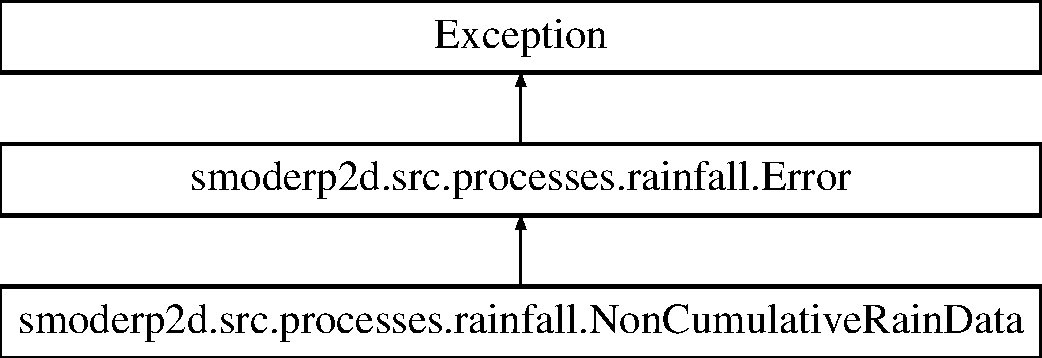
\includegraphics[height=3.000000cm]{classsmoderp2d_1_1src_1_1processes_1_1rainfall_1_1NonCumulativeRainData}
\end{center}
\end{figure}
\subsection*{Public Member Functions}
\begin{DoxyCompactItemize}
\item 
\hypertarget{classsmoderp2d_1_1src_1_1processes_1_1rainfall_1_1NonCumulativeRainData_a8c1819953f50758356fecb2e21298949}{def {\bfseries \-\_\-\-\_\-init\-\_\-\-\_\-}}\label{classsmoderp2d_1_1src_1_1processes_1_1rainfall_1_1NonCumulativeRainData_a8c1819953f50758356fecb2e21298949}

\item 
\hypertarget{classsmoderp2d_1_1src_1_1processes_1_1rainfall_1_1NonCumulativeRainData_ae724b18ea56d343746cdcec410a591fe}{def {\bfseries \-\_\-\-\_\-str\-\_\-\-\_\-}}\label{classsmoderp2d_1_1src_1_1processes_1_1rainfall_1_1NonCumulativeRainData_ae724b18ea56d343746cdcec410a591fe}

\end{DoxyCompactItemize}
\subsection*{Public Attributes}
\begin{DoxyCompactItemize}
\item 
\hypertarget{classsmoderp2d_1_1src_1_1processes_1_1rainfall_1_1NonCumulativeRainData_a238df79989636c9e0df402640d1d2a57}{{\bfseries msg}}\label{classsmoderp2d_1_1src_1_1processes_1_1rainfall_1_1NonCumulativeRainData_a238df79989636c9e0df402640d1d2a57}

\end{DoxyCompactItemize}


\subsection{Detailed Description}
\begin{DoxyVerb}Exception raised bad rainfall record assignment.

Attributes:
    msg  -- explanation of the error
\end{DoxyVerb}
 

The documentation for this class was generated from the following file\-:\begin{DoxyCompactItemize}
\item 
smoderp2d/src/processes/rainfall.\-py\end{DoxyCompactItemize}

\hypertarget{classsmoderp2d_1_1src_1_1data__preparation_1_1Outlet}{\section{smoderp2d.\-src.\-data\-\_\-preparation.\-Outlet Class Reference}
\label{classsmoderp2d_1_1src_1_1data__preparation_1_1Outlet}\index{smoderp2d.\-src.\-data\-\_\-preparation.\-Outlet@{smoderp2d.\-src.\-data\-\_\-preparation.\-Outlet}}
}


Class to find out the possible catchment outlets.  


\subsection*{Public Member Functions}
\begin{DoxyCompactItemize}
\item 
\hypertarget{classsmoderp2d_1_1src_1_1data__preparation_1_1Outlet_a38d7640690632fb70da2cb968d1c4320}{def \hyperlink{classsmoderp2d_1_1src_1_1data__preparation_1_1Outlet_a38d7640690632fb70da2cb968d1c4320}{\-\_\-\-\_\-init\-\_\-\-\_\-}}\label{classsmoderp2d_1_1src_1_1data__preparation_1_1Outlet_a38d7640690632fb70da2cb968d1c4320}

\begin{DoxyCompactList}\small\item\em constructor \end{DoxyCompactList}\item 
\hypertarget{classsmoderp2d_1_1src_1_1data__preparation_1_1Outlet_a3371e5c1451c87f332ac83cdf8196bb1}{def \hyperlink{classsmoderp2d_1_1src_1_1data__preparation_1_1Outlet_a3371e5c1451c87f332ac83cdf8196bb1}{push}}\label{classsmoderp2d_1_1src_1_1data__preparation_1_1Outlet_a3371e5c1451c87f332ac83cdf8196bb1}

\begin{DoxyCompactList}\small\item\em Function to determine cells indexes and neighbor of all cells in the domain. \end{DoxyCompactList}\item 
def \hyperlink{classsmoderp2d_1_1src_1_1data__preparation_1_1Outlet_a2243e5b391c4db099fc2876f09b7ef28}{find\-\_\-outlets}
\begin{DoxyCompactList}\small\item\em Determine which of cells in the domain are outlet. \end{DoxyCompactList}\end{DoxyCompactItemize}
\subsection*{Public Attributes}
\begin{DoxyCompactItemize}
\item 
\hypertarget{classsmoderp2d_1_1src_1_1data__preparation_1_1Outlet_ac0532eb0756f3428f6180c86101eec10}{\hyperlink{classsmoderp2d_1_1src_1_1data__preparation_1_1Outlet_ac0532eb0756f3428f6180c86101eec10}{cell}}\label{classsmoderp2d_1_1src_1_1data__preparation_1_1Outlet_ac0532eb0756f3428f6180c86101eec10}

\begin{DoxyCompactList}\small\item\em cells in the domain \end{DoxyCompactList}\item 
\hypertarget{classsmoderp2d_1_1src_1_1data__preparation_1_1Outlet_a386a5fd492d80579f104fa0c35748316}{{\bfseries cell\-Neighbour}}\label{classsmoderp2d_1_1src_1_1data__preparation_1_1Outlet_a386a5fd492d80579f104fa0c35748316}

\item 
\hypertarget{classsmoderp2d_1_1src_1_1data__preparation_1_1Outlet_ab1d5f3c1eac7cbb99df52f7478415505}{{\bfseries outlet\-Cells}}\label{classsmoderp2d_1_1src_1_1data__preparation_1_1Outlet_ab1d5f3c1eac7cbb99df52f7478415505}

\end{DoxyCompactItemize}


\subsection{Detailed Description}
Class to find out the possible catchment outlets. 

\subsection{Member Function Documentation}
\hypertarget{classsmoderp2d_1_1src_1_1data__preparation_1_1Outlet_a2243e5b391c4db099fc2876f09b7ef28}{\index{smoderp2d\-::src\-::data\-\_\-preparation\-::\-Outlet@{smoderp2d\-::src\-::data\-\_\-preparation\-::\-Outlet}!find\-\_\-outlets@{find\-\_\-outlets}}
\index{find\-\_\-outlets@{find\-\_\-outlets}!smoderp2d::src::data_preparation::Outlet@{smoderp2d\-::src\-::data\-\_\-preparation\-::\-Outlet}}
\subsubsection[{find\-\_\-outlets}]{\setlength{\rightskip}{0pt plus 5cm}def smoderp2d.\-src.\-data\-\_\-preparation.\-Outlet.\-find\-\_\-outlets (
\begin{DoxyParamCaption}
\item[{}]{self, }
\item[{}]{dem}
\end{DoxyParamCaption}
)}}\label{classsmoderp2d_1_1src_1_1data__preparation_1_1Outlet_a2243e5b391c4db099fc2876f09b7ef28}


Determine which of cells in the domain are outlet. 

\hyperlink{classsmoderp2d_1_1src_1_1data__preparation_1_1Outlet}{Outlet} cell is the lowers cell compared to all its neighbors 

The documentation for this class was generated from the following file\-:\begin{DoxyCompactItemize}
\item 
smoderp2d/src/data\-\_\-preparation.\-py\end{DoxyCompactItemize}

\hypertarget{classsmoderp2d_1_1src_1_1main__classes_1_1Stream_1_1Reach}{\section{smoderp2d.\-src.\-main\-\_\-classes.\-Stream.\-Reach Class Reference}
\label{classsmoderp2d_1_1src_1_1main__classes_1_1Stream_1_1Reach}\index{smoderp2d.\-src.\-main\-\_\-classes.\-Stream.\-Reach@{smoderp2d.\-src.\-main\-\_\-classes.\-Stream.\-Reach}}
}
\subsection*{Public Member Functions}
\begin{DoxyCompactItemize}
\item 
\hypertarget{classsmoderp2d_1_1src_1_1main__classes_1_1Stream_1_1Reach_af14efa37bb1c8fb9ec37a8bf0198da35}{def {\bfseries \-\_\-\-\_\-init\-\_\-\-\_\-}}\label{classsmoderp2d_1_1src_1_1main__classes_1_1Stream_1_1Reach_af14efa37bb1c8fb9ec37a8bf0198da35}

\end{DoxyCompactItemize}
\subsection*{Public Attributes}
\begin{DoxyCompactItemize}
\item 
\hypertarget{classsmoderp2d_1_1src_1_1main__classes_1_1Stream_1_1Reach_a99ab17b778f4d172df8242e4511b1154}{{\bfseries id\-\_\-}}\label{classsmoderp2d_1_1src_1_1main__classes_1_1Stream_1_1Reach_a99ab17b778f4d172df8242e4511b1154}

\item 
\hypertarget{classsmoderp2d_1_1src_1_1main__classes_1_1Stream_1_1Reach_a769dbb74602a30d9362ac198f9196a8c}{\hyperlink{classsmoderp2d_1_1src_1_1main__classes_1_1Stream_1_1Reach_a769dbb74602a30d9362ac198f9196a8c}{points\-From}}\label{classsmoderp2d_1_1src_1_1main__classes_1_1Stream_1_1Reach_a769dbb74602a30d9362ac198f9196a8c}

\begin{DoxyCompactList}\small\item\em self.\-imat = i \#jj melo byt pozice v matici, ale to mozna nani treba kdyz zanech mat\-\_\-tok\-\_\-usek a tam id useku self.\-jmat = j \end{DoxyCompactList}\item 
\hypertarget{classsmoderp2d_1_1src_1_1main__classes_1_1Stream_1_1Reach_a5dad84169dbde000b98548110fddc07c}{{\bfseries points\-To}}\label{classsmoderp2d_1_1src_1_1main__classes_1_1Stream_1_1Reach_a5dad84169dbde000b98548110fddc07c}

\item 
\hypertarget{classsmoderp2d_1_1src_1_1main__classes_1_1Stream_1_1Reach_a2e0ae29b0fcca2a4ed0a174cf8ec8e6d}{{\bfseries to\-\_\-node}}\label{classsmoderp2d_1_1src_1_1main__classes_1_1Stream_1_1Reach_a2e0ae29b0fcca2a4ed0a174cf8ec8e6d}

\item 
\hypertarget{classsmoderp2d_1_1src_1_1main__classes_1_1Stream_1_1Reach_a2a612825ef5da7cd6bdcdd4473ba60bd}{{\bfseries length}}\label{classsmoderp2d_1_1src_1_1main__classes_1_1Stream_1_1Reach_a2a612825ef5da7cd6bdcdd4473ba60bd}

\item 
\hypertarget{classsmoderp2d_1_1src_1_1main__classes_1_1Stream_1_1Reach_a995ac67994ec01bf105eb5cf4c2afb01}{{\bfseries slope}}\label{classsmoderp2d_1_1src_1_1main__classes_1_1Stream_1_1Reach_a995ac67994ec01bf105eb5cf4c2afb01}

\item 
\hypertarget{classsmoderp2d_1_1src_1_1main__classes_1_1Stream_1_1Reach_a2aeb56b0125c4d5b0ff7847cac91384c}{{\bfseries smoderp}}\label{classsmoderp2d_1_1src_1_1main__classes_1_1Stream_1_1Reach_a2aeb56b0125c4d5b0ff7847cac91384c}

\item 
\hypertarget{classsmoderp2d_1_1src_1_1main__classes_1_1Stream_1_1Reach_ab67c4773cf1c3670df5fe875d5f1c962}{{\bfseries no}}\label{classsmoderp2d_1_1src_1_1main__classes_1_1Stream_1_1Reach_ab67c4773cf1c3670df5fe875d5f1c962}

\item 
\hypertarget{classsmoderp2d_1_1src_1_1main__classes_1_1Stream_1_1Reach_a3e41520f1c712f581ba8628e8e87737c}{{\bfseries shape}}\label{classsmoderp2d_1_1src_1_1main__classes_1_1Stream_1_1Reach_a3e41520f1c712f581ba8628e8e87737c}

\item 
\hypertarget{classsmoderp2d_1_1src_1_1main__classes_1_1Stream_1_1Reach_a8525382a4fce57bdbb9e4531e29afee6}{{\bfseries b}}\label{classsmoderp2d_1_1src_1_1main__classes_1_1Stream_1_1Reach_a8525382a4fce57bdbb9e4531e29afee6}

\item 
\hypertarget{classsmoderp2d_1_1src_1_1main__classes_1_1Stream_1_1Reach_a3f7e54af0bbca4cb75e6d19c80ec67bc}{{\bfseries m}}\label{classsmoderp2d_1_1src_1_1main__classes_1_1Stream_1_1Reach_a3f7e54af0bbca4cb75e6d19c80ec67bc}

\item 
\hypertarget{classsmoderp2d_1_1src_1_1main__classes_1_1Stream_1_1Reach_a3c6d9ab34e9c9d1fdaadc7f733a29c23}{{\bfseries roughness}}\label{classsmoderp2d_1_1src_1_1main__classes_1_1Stream_1_1Reach_a3c6d9ab34e9c9d1fdaadc7f733a29c23}

\item 
\hypertarget{classsmoderp2d_1_1src_1_1main__classes_1_1Stream_1_1Reach_a8df80a9e36538e1ed6200f5e9b612b2b}{{\bfseries Q365}}\label{classsmoderp2d_1_1src_1_1main__classes_1_1Stream_1_1Reach_a8df80a9e36538e1ed6200f5e9b612b2b}

\item 
\hypertarget{classsmoderp2d_1_1src_1_1main__classes_1_1Stream_1_1Reach_adf7935aa0d4c8f459187202c45ef8d8b}{{\bfseries V\-\_\-in\-\_\-from\-\_\-field}}\label{classsmoderp2d_1_1src_1_1main__classes_1_1Stream_1_1Reach_adf7935aa0d4c8f459187202c45ef8d8b}

\item 
\hypertarget{classsmoderp2d_1_1src_1_1main__classes_1_1Stream_1_1Reach_aaf45b921972fe753ae78d468be035095}{{\bfseries V\-\_\-in\-\_\-from\-\_\-field\-\_\-cum}}\label{classsmoderp2d_1_1src_1_1main__classes_1_1Stream_1_1Reach_aaf45b921972fe753ae78d468be035095}

\item 
\hypertarget{classsmoderp2d_1_1src_1_1main__classes_1_1Stream_1_1Reach_a830b0ed75bc9d4670841157ff4b038d2}{{\bfseries V\-\_\-in\-\_\-from\-\_\-reach}}\label{classsmoderp2d_1_1src_1_1main__classes_1_1Stream_1_1Reach_a830b0ed75bc9d4670841157ff4b038d2}

\item 
\hypertarget{classsmoderp2d_1_1src_1_1main__classes_1_1Stream_1_1Reach_a63a213ec9d170215cbc6aae2f5fb7d9f}{{\bfseries V\-\_\-out\-\_\-cum}}\label{classsmoderp2d_1_1src_1_1main__classes_1_1Stream_1_1Reach_a63a213ec9d170215cbc6aae2f5fb7d9f}

\item 
\hypertarget{classsmoderp2d_1_1src_1_1main__classes_1_1Stream_1_1Reach_a7bc6582f7505682a3964912f375d812a}{{\bfseries V\-\_\-rest}}\label{classsmoderp2d_1_1src_1_1main__classes_1_1Stream_1_1Reach_a7bc6582f7505682a3964912f375d812a}

\item 
\hypertarget{classsmoderp2d_1_1src_1_1main__classes_1_1Stream_1_1Reach_a101766b76314335edefbc711082664f6}{{\bfseries h}}\label{classsmoderp2d_1_1src_1_1main__classes_1_1Stream_1_1Reach_a101766b76314335edefbc711082664f6}

\item 
\hypertarget{classsmoderp2d_1_1src_1_1main__classes_1_1Stream_1_1Reach_a2120a26ee4f29e2bc258e01d360dfb99}{{\bfseries h\-\_\-max}}\label{classsmoderp2d_1_1src_1_1main__classes_1_1Stream_1_1Reach_a2120a26ee4f29e2bc258e01d360dfb99}

\item 
\hypertarget{classsmoderp2d_1_1src_1_1main__classes_1_1Stream_1_1Reach_aa84be3efc5d5e9d369db57f4842e6371}{{\bfseries timeh\-\_\-max}}\label{classsmoderp2d_1_1src_1_1main__classes_1_1Stream_1_1Reach_aa84be3efc5d5e9d369db57f4842e6371}

\item 
\hypertarget{classsmoderp2d_1_1src_1_1main__classes_1_1Stream_1_1Reach_a09f67a2267f2c1e84e7f73961ad5953d}{{\bfseries V\-\_\-out}}\label{classsmoderp2d_1_1src_1_1main__classes_1_1Stream_1_1Reach_a09f67a2267f2c1e84e7f73961ad5953d}

\item 
\hypertarget{classsmoderp2d_1_1src_1_1main__classes_1_1Stream_1_1Reach_a91c2465a45fe4a86d253dc395dd5997f}{{\bfseries vs}}\label{classsmoderp2d_1_1src_1_1main__classes_1_1Stream_1_1Reach_a91c2465a45fe4a86d253dc395dd5997f}

\item 
\hypertarget{classsmoderp2d_1_1src_1_1main__classes_1_1Stream_1_1Reach_a785efe7c4789aecde61dc6455b9ff10a}{{\bfseries Q\-\_\-out}}\label{classsmoderp2d_1_1src_1_1main__classes_1_1Stream_1_1Reach_a785efe7c4789aecde61dc6455b9ff10a}

\item 
\hypertarget{classsmoderp2d_1_1src_1_1main__classes_1_1Stream_1_1Reach_a144bad92701e39e1dc85f5d0c296612f}{{\bfseries Q\-\_\-max}}\label{classsmoderp2d_1_1src_1_1main__classes_1_1Stream_1_1Reach_a144bad92701e39e1dc85f5d0c296612f}

\item 
\hypertarget{classsmoderp2d_1_1src_1_1main__classes_1_1Stream_1_1Reach_a2288c527275d3c1f29b4f9b4d7ba10ae}{{\bfseries time\-Q\-\_\-max}}\label{classsmoderp2d_1_1src_1_1main__classes_1_1Stream_1_1Reach_a2288c527275d3c1f29b4f9b4d7ba10ae}

\item 
\hypertarget{classsmoderp2d_1_1src_1_1main__classes_1_1Stream_1_1Reach_afa1bc9e1ee93bf29c4d2a1585a9ca800}{{\bfseries V\-\_\-out\-\_\-domain}}\label{classsmoderp2d_1_1src_1_1main__classes_1_1Stream_1_1Reach_afa1bc9e1ee93bf29c4d2a1585a9ca800}

\item 
\hypertarget{classsmoderp2d_1_1src_1_1main__classes_1_1Stream_1_1Reach_ae43e6508ba3aead29d195425d3b342c2}{{\bfseries outflow\-\_\-method}}\label{classsmoderp2d_1_1src_1_1main__classes_1_1Stream_1_1Reach_ae43e6508ba3aead29d195425d3b342c2}

\end{DoxyCompactItemize}


The documentation for this class was generated from the following file\-:\begin{DoxyCompactItemize}
\item 
smoderp2d/src/main\-\_\-classes/Stream.\-py\end{DoxyCompactItemize}

\hypertarget{classsmoderp2d_1_1src_1_1runoff_1_1Runoff}{\section{smoderp2d.\-src.\-runoff.\-Runoff Class Reference}
\label{classsmoderp2d_1_1src_1_1runoff_1_1Runoff}\index{smoderp2d.\-src.\-runoff.\-Runoff@{smoderp2d.\-src.\-runoff.\-Runoff}}
}
\subsection*{Public Member Functions}
\begin{DoxyCompactItemize}
\item 
\hypertarget{classsmoderp2d_1_1src_1_1runoff_1_1Runoff_a2c45be9fe5ed3087844b8712830865e4}{def {\bfseries run}}\label{classsmoderp2d_1_1src_1_1runoff_1_1Runoff_a2c45be9fe5ed3087844b8712830865e4}

\end{DoxyCompactItemize}


\subsection{Detailed Description}


Definition at line 135 of file runoff.\-py.



The documentation for this class was generated from the following file\-:\begin{DoxyCompactItemize}
\item 
smoderp2d/src/runoff.\-py\end{DoxyCompactItemize}

\hypertarget{classsmoderp2d_1_1src_1_1tools_1_1save__load__data__nopickle_1_1SaveItems}{\section{smoderp2d.\-src.\-tools.\-save\-\_\-load\-\_\-data\-\_\-nopickle.\-Save\-Items Class Reference}
\label{classsmoderp2d_1_1src_1_1tools_1_1save__load__data__nopickle_1_1SaveItems}\index{smoderp2d.\-src.\-tools.\-save\-\_\-load\-\_\-data\-\_\-nopickle.\-Save\-Items@{smoderp2d.\-src.\-tools.\-save\-\_\-load\-\_\-data\-\_\-nopickle.\-Save\-Items}}
}


Class to save item of different typy.  


Inheritance diagram for smoderp2d.\-src.\-tools.\-save\-\_\-load\-\_\-data\-\_\-nopickle.\-Save\-Items\-:\begin{figure}[H]
\begin{center}
\leavevmode
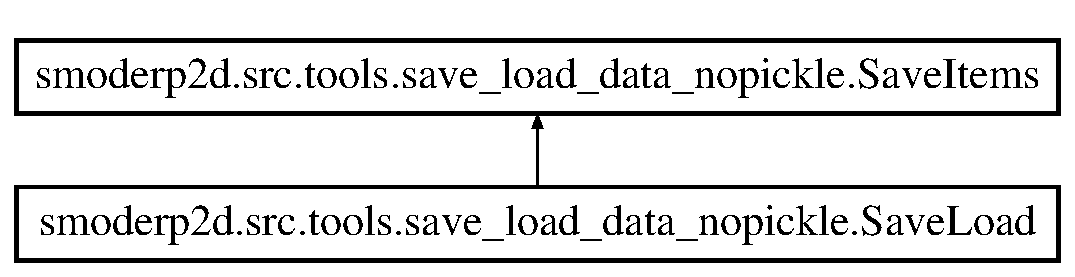
\includegraphics[height=2.000000cm]{classsmoderp2d_1_1src_1_1tools_1_1save__load__data__nopickle_1_1SaveItems}
\end{center}
\end{figure}
\subsection*{Public Member Functions}
\begin{DoxyCompactItemize}
\item 
\hypertarget{classsmoderp2d_1_1src_1_1tools_1_1save__load__data__nopickle_1_1SaveItems_a9b7ab58852c2ec9ac5eef3697891a971}{def {\bfseries savelist}}\label{classsmoderp2d_1_1src_1_1tools_1_1save__load__data__nopickle_1_1SaveItems_a9b7ab58852c2ec9ac5eef3697891a971}

\item 
\hypertarget{classsmoderp2d_1_1src_1_1tools_1_1save__load__data__nopickle_1_1SaveItems_aae4bd717ff245f0866e1a3d2344f6e88}{def {\bfseries saveint}}\label{classsmoderp2d_1_1src_1_1tools_1_1save__load__data__nopickle_1_1SaveItems_aae4bd717ff245f0866e1a3d2344f6e88}

\item 
\hypertarget{classsmoderp2d_1_1src_1_1tools_1_1save__load__data__nopickle_1_1SaveItems_aaa5119329a342c10796e2bbbe43a4c04}{def {\bfseries savefloat}}\label{classsmoderp2d_1_1src_1_1tools_1_1save__load__data__nopickle_1_1SaveItems_aaa5119329a342c10796e2bbbe43a4c04}

\item 
\hypertarget{classsmoderp2d_1_1src_1_1tools_1_1save__load__data__nopickle_1_1SaveItems_a9aeb5708cc4eec875ecdde27a41359b1}{def {\bfseries savestr}}\label{classsmoderp2d_1_1src_1_1tools_1_1save__load__data__nopickle_1_1SaveItems_a9aeb5708cc4eec875ecdde27a41359b1}

\item 
\hypertarget{classsmoderp2d_1_1src_1_1tools_1_1save__load__data__nopickle_1_1SaveItems_aec22b79dd1a286a28cd142ddd07deaae}{def {\bfseries saveunicode}}\label{classsmoderp2d_1_1src_1_1tools_1_1save__load__data__nopickle_1_1SaveItems_aec22b79dd1a286a28cd142ddd07deaae}

\item 
\hypertarget{classsmoderp2d_1_1src_1_1tools_1_1save__load__data__nopickle_1_1SaveItems_ac9ca6022e3f3045e5bd4a1327656ee63}{def {\bfseries savenumpy}}\label{classsmoderp2d_1_1src_1_1tools_1_1save__load__data__nopickle_1_1SaveItems_ac9ca6022e3f3045e5bd4a1327656ee63}

\end{DoxyCompactItemize}


\subsection{Detailed Description}
Class to save item of different typy. 

The documentation for this class was generated from the following file\-:\begin{DoxyCompactItemize}
\item 
smoderp2d/src/tools/save\-\_\-load\-\_\-data\-\_\-nopickle.\-py\end{DoxyCompactItemize}

\hypertarget{classsmoderp2d_1_1src_1_1tools_1_1savezipconvert_1_1SaveItems}{\section{smoderp2d.\-src.\-tools.\-savezipconvert.\-Save\-Items Class Reference}
\label{classsmoderp2d_1_1src_1_1tools_1_1savezipconvert_1_1SaveItems}\index{smoderp2d.\-src.\-tools.\-savezipconvert.\-Save\-Items@{smoderp2d.\-src.\-tools.\-savezipconvert.\-Save\-Items}}
}
Inheritance diagram for smoderp2d.\-src.\-tools.\-savezipconvert.\-Save\-Items\-:\begin{figure}[H]
\begin{center}
\leavevmode
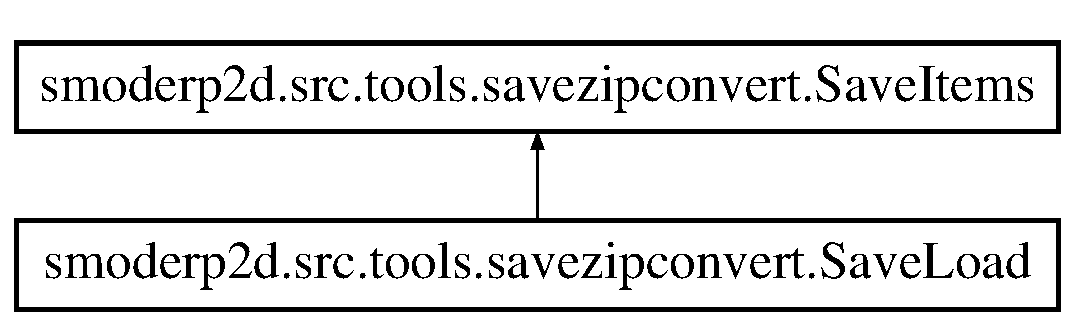
\includegraphics[height=2.000000cm]{d0/ddc/classsmoderp2d_1_1src_1_1tools_1_1savezipconvert_1_1SaveItems}
\end{center}
\end{figure}
\subsection*{Public Member Functions}
\begin{DoxyCompactItemize}
\item 
\hypertarget{classsmoderp2d_1_1src_1_1tools_1_1savezipconvert_1_1SaveItems_a88cd7dcb985be92294af1443ecf46573}{def {\bfseries savelist}}\label{classsmoderp2d_1_1src_1_1tools_1_1savezipconvert_1_1SaveItems_a88cd7dcb985be92294af1443ecf46573}

\item 
\hypertarget{classsmoderp2d_1_1src_1_1tools_1_1savezipconvert_1_1SaveItems_abffb863fffb5c4184101afdb2c343119}{def {\bfseries saveint}}\label{classsmoderp2d_1_1src_1_1tools_1_1savezipconvert_1_1SaveItems_abffb863fffb5c4184101afdb2c343119}

\item 
\hypertarget{classsmoderp2d_1_1src_1_1tools_1_1savezipconvert_1_1SaveItems_a89063838b17949e6152947ce1f3ef90b}{def {\bfseries savefloat}}\label{classsmoderp2d_1_1src_1_1tools_1_1savezipconvert_1_1SaveItems_a89063838b17949e6152947ce1f3ef90b}

\item 
\hypertarget{classsmoderp2d_1_1src_1_1tools_1_1savezipconvert_1_1SaveItems_a8b9a04c1bda1b67c17a8f680ab6a83c9}{def {\bfseries savestr}}\label{classsmoderp2d_1_1src_1_1tools_1_1savezipconvert_1_1SaveItems_a8b9a04c1bda1b67c17a8f680ab6a83c9}

\item 
\hypertarget{classsmoderp2d_1_1src_1_1tools_1_1savezipconvert_1_1SaveItems_a95863c1b617a2cfecf2502a1150651d8}{def {\bfseries saveunicode}}\label{classsmoderp2d_1_1src_1_1tools_1_1savezipconvert_1_1SaveItems_a95863c1b617a2cfecf2502a1150651d8}

\item 
\hypertarget{classsmoderp2d_1_1src_1_1tools_1_1savezipconvert_1_1SaveItems_a17acf5ee275ad2da8483d2624d983bf1}{def {\bfseries savenumpy}}\label{classsmoderp2d_1_1src_1_1tools_1_1savezipconvert_1_1SaveItems_a17acf5ee275ad2da8483d2624d983bf1}

\end{DoxyCompactItemize}


\subsection{Detailed Description}


Definition at line 22 of file savezipconvert.\-py.



The documentation for this class was generated from the following file\-:\begin{DoxyCompactItemize}
\item 
smoderp2d/src/tools/savezipconvert.\-py\end{DoxyCompactItemize}

\hypertarget{classsmoderp2d_1_1src_1_1tools_1_1savezipconvert_1_1SaveLoad}{\section{smoderp2d.\-src.\-tools.\-savezipconvert.\-Save\-Load Class Reference}
\label{classsmoderp2d_1_1src_1_1tools_1_1savezipconvert_1_1SaveLoad}\index{smoderp2d.\-src.\-tools.\-savezipconvert.\-Save\-Load@{smoderp2d.\-src.\-tools.\-savezipconvert.\-Save\-Load}}
}
Inheritance diagram for smoderp2d.\-src.\-tools.\-savezipconvert.\-Save\-Load\-:\begin{figure}[H]
\begin{center}
\leavevmode
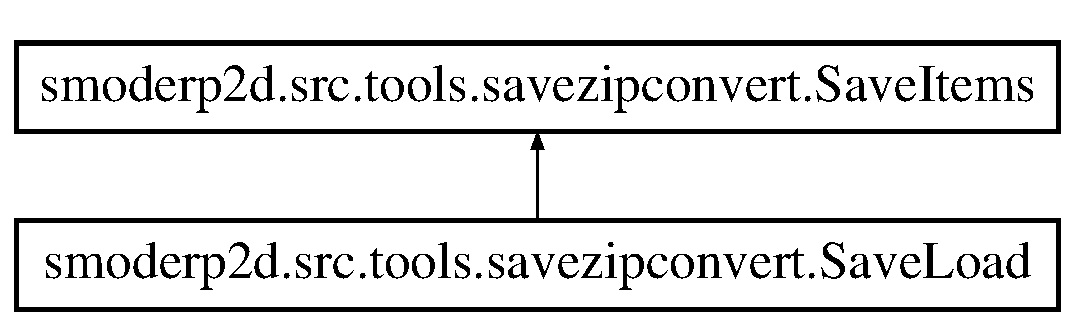
\includegraphics[height=2.000000cm]{classsmoderp2d_1_1src_1_1tools_1_1savezipconvert_1_1SaveLoad}
\end{center}
\end{figure}
\subsection*{Public Member Functions}
\begin{DoxyCompactItemize}
\item 
\hypertarget{classsmoderp2d_1_1src_1_1tools_1_1savezipconvert_1_1SaveLoad_a054ff307ab4f5403c31243f9d00eb953}{def {\bfseries save}}\label{classsmoderp2d_1_1src_1_1tools_1_1savezipconvert_1_1SaveLoad_a054ff307ab4f5403c31243f9d00eb953}

\item 
\hypertarget{classsmoderp2d_1_1src_1_1tools_1_1savezipconvert_1_1SaveLoad_a3ab39289191759cf2f7159c9dca7f83a}{def {\bfseries save\-\_\-item}}\label{classsmoderp2d_1_1src_1_1tools_1_1savezipconvert_1_1SaveLoad_a3ab39289191759cf2f7159c9dca7f83a}

\end{DoxyCompactItemize}
\subsection*{Public Attributes}
\begin{DoxyCompactItemize}
\item 
\hypertarget{classsmoderp2d_1_1src_1_1tools_1_1savezipconvert_1_1SaveLoad_af128345f0d5fc0833600801586caebe8}{{\bfseries count\-List}}\label{classsmoderp2d_1_1src_1_1tools_1_1savezipconvert_1_1SaveLoad_af128345f0d5fc0833600801586caebe8}

\end{DoxyCompactItemize}


The documentation for this class was generated from the following file\-:\begin{DoxyCompactItemize}
\item 
smoderp2d/src/tools/savezipconvert.\-py\end{DoxyCompactItemize}

\hypertarget{classsmoderp2d_1_1src_1_1tools_1_1save__load__data__nopickle_1_1SaveLoad}{\section{smoderp2d.\-src.\-tools.\-save\-\_\-load\-\_\-data\-\_\-nopickle.\-Save\-Load Class Reference}
\label{classsmoderp2d_1_1src_1_1tools_1_1save__load__data__nopickle_1_1SaveLoad}\index{smoderp2d.\-src.\-tools.\-save\-\_\-load\-\_\-data\-\_\-nopickle.\-Save\-Load@{smoderp2d.\-src.\-tools.\-save\-\_\-load\-\_\-data\-\_\-nopickle.\-Save\-Load}}
}


Class to save and load the data returned from the datapreparation in and from zip archive.  


Inheritance diagram for smoderp2d.\-src.\-tools.\-save\-\_\-load\-\_\-data\-\_\-nopickle.\-Save\-Load\-:\begin{figure}[H]
\begin{center}
\leavevmode
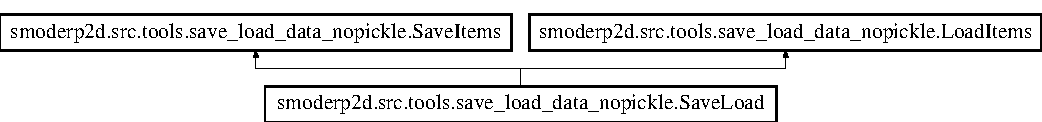
\includegraphics[height=1.637427cm]{classsmoderp2d_1_1src_1_1tools_1_1save__load__data__nopickle_1_1SaveLoad}
\end{center}
\end{figure}
\subsection*{Public Member Functions}
\begin{DoxyCompactItemize}
\item 
\hypertarget{classsmoderp2d_1_1src_1_1tools_1_1save__load__data__nopickle_1_1SaveLoad_a31316039ba0bb03ae075194fa64cfa41}{def {\bfseries save}}\label{classsmoderp2d_1_1src_1_1tools_1_1save__load__data__nopickle_1_1SaveLoad_a31316039ba0bb03ae075194fa64cfa41}

\item 
\hypertarget{classsmoderp2d_1_1src_1_1tools_1_1save__load__data__nopickle_1_1SaveLoad_a5c3b185f5ac9e5906b49d6cac5b7e02a}{def {\bfseries load}}\label{classsmoderp2d_1_1src_1_1tools_1_1save__load__data__nopickle_1_1SaveLoad_a5c3b185f5ac9e5906b49d6cac5b7e02a}

\item 
\hypertarget{classsmoderp2d_1_1src_1_1tools_1_1save__load__data__nopickle_1_1SaveLoad_a4998bf25b098e24c409bbc0f26722964}{def {\bfseries save\-\_\-item}}\label{classsmoderp2d_1_1src_1_1tools_1_1save__load__data__nopickle_1_1SaveLoad_a4998bf25b098e24c409bbc0f26722964}

\item 
\hypertarget{classsmoderp2d_1_1src_1_1tools_1_1save__load__data__nopickle_1_1SaveLoad_a85f4c4638f570a6b276f58026a004ac9}{def {\bfseries load\-\_\-item}}\label{classsmoderp2d_1_1src_1_1tools_1_1save__load__data__nopickle_1_1SaveLoad_a85f4c4638f570a6b276f58026a004ac9}

\end{DoxyCompactItemize}
\subsection*{Public Attributes}
\begin{DoxyCompactItemize}
\item 
\hypertarget{classsmoderp2d_1_1src_1_1tools_1_1save__load__data__nopickle_1_1SaveLoad_ad3bed899b380199e62bed31b6d40f0f2}{{\bfseries count\-List}}\label{classsmoderp2d_1_1src_1_1tools_1_1save__load__data__nopickle_1_1SaveLoad_ad3bed899b380199e62bed31b6d40f0f2}

\item 
\hypertarget{classsmoderp2d_1_1src_1_1tools_1_1save__load__data__nopickle_1_1SaveLoad_a3101022a38b6b958d8a05909b71208fb}{{\bfseries lines}}\label{classsmoderp2d_1_1src_1_1tools_1_1save__load__data__nopickle_1_1SaveLoad_a3101022a38b6b958d8a05909b71208fb}

\end{DoxyCompactItemize}


\subsection{Detailed Description}
Class to save and load the data returned from the datapreparation in and from zip archive. 

The documentation for this class was generated from the following file\-:\begin{DoxyCompactItemize}
\item 
smoderp2d/src/tools/save\-\_\-load\-\_\-data\-\_\-nopickle.\-py\end{DoxyCompactItemize}

\hypertarget{classsmoderp2d_1_1src_1_1main__classes_1_1General_1_1Size}{\section{smoderp2d.\-src.\-main\-\_\-classes.\-General.\-Size Class Reference}
\label{classsmoderp2d_1_1src_1_1main__classes_1_1General_1_1Size}\index{smoderp2d.\-src.\-main\-\_\-classes.\-General.\-Size@{smoderp2d.\-src.\-main\-\_\-classes.\-General.\-Size}}
}


Documentation for a class.  


Inheritance diagram for smoderp2d.\-src.\-main\-\_\-classes.\-General.\-Size\-:\begin{figure}[H]
\begin{center}
\leavevmode
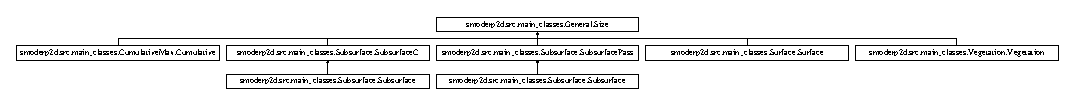
\includegraphics[height=0.965517cm]{d6/de2/classsmoderp2d_1_1src_1_1main__classes_1_1General_1_1Size}
\end{center}
\end{figure}
\subsection*{Public Member Functions}
\begin{DoxyCompactItemize}
\item 
def \hyperlink{classsmoderp2d_1_1src_1_1main__classes_1_1General_1_1Size_a8546bcd644a0f79337648b9b1badaf4a}{size}
\begin{DoxyCompactList}\small\item\em size \end{DoxyCompactList}\end{DoxyCompactItemize}


\subsection{Detailed Description}
Documentation for a class. 

method to compute size of class arrays 

Definition at line 21 of file General.\-py.



\subsection{Member Function Documentation}
\hypertarget{classsmoderp2d_1_1src_1_1main__classes_1_1General_1_1Size_a8546bcd644a0f79337648b9b1badaf4a}{\index{smoderp2d\-::src\-::main\-\_\-classes\-::\-General\-::\-Size@{smoderp2d\-::src\-::main\-\_\-classes\-::\-General\-::\-Size}!size@{size}}
\index{size@{size}!smoderp2d::src::main_classes::General::Size@{smoderp2d\-::src\-::main\-\_\-classes\-::\-General\-::\-Size}}
\subsubsection[{size}]{\setlength{\rightskip}{0pt plus 5cm}def smoderp2d.\-src.\-main\-\_\-classes.\-General.\-Size.\-size (
\begin{DoxyParamCaption}
\item[{}]{self, }
\item[{}]{array\-N\-Bytes, }
\item[{}]{m = {\ttfamily 1.0}}
\end{DoxyParamCaption}
)}}\label{classsmoderp2d_1_1src_1_1main__classes_1_1General_1_1Size_a8546bcd644a0f79337648b9b1badaf4a}


size 


\begin{DoxyParams}{Parameters}
{\em array\-N\-Bytes} & $<$numpy array$>$=\char`\"{}\char`\"{}$>$.nbytes \\
\hline
{\em m} & value in denominator to get bytes, kilobytes (m=2$\ast$$\ast$10), megabytes (m=2$\ast$$\ast$10+m$\ast$$\ast$10) and so on. \\
\hline
\end{DoxyParams}


Definition at line 26 of file General.\-py.


\begin{DoxyCode}
26 
27   \textcolor{keyword}{def }\hyperlink{classsmoderp2d_1_1src_1_1main__classes_1_1General_1_1Size_a8546bcd644a0f79337648b9b1badaf4a}{size}(self, arrayNBytes, m=1.0):
28     \textcolor{comment}{# arrayNBytes eq self.state.nbytes}
29     size = (self.n * arrayNBytes)/m
30     \textcolor{keywordflow}{return} size
31 
32 
33 
34 
35 
36 
37 
38 
39 

\end{DoxyCode}


The documentation for this class was generated from the following file\-:\begin{DoxyCompactItemize}
\item 
smoderp2d/src/main\-\_\-classes/General.\-py\end{DoxyCompactItemize}

\hypertarget{classsmoderp2d_1_1src_1_1main__classes_1_1Stream_1_1Stream}{\section{smoderp2d.\-src.\-main\-\_\-classes.\-Stream.\-Stream Class Reference}
\label{classsmoderp2d_1_1src_1_1main__classes_1_1Stream_1_1Stream}\index{smoderp2d.\-src.\-main\-\_\-classes.\-Stream.\-Stream@{smoderp2d.\-src.\-main\-\_\-classes.\-Stream.\-Stream}}
}


Documentation for a class.  


Inheritance diagram for smoderp2d.\-src.\-main\-\_\-classes.\-Stream.\-Stream\-:\begin{figure}[H]
\begin{center}
\leavevmode
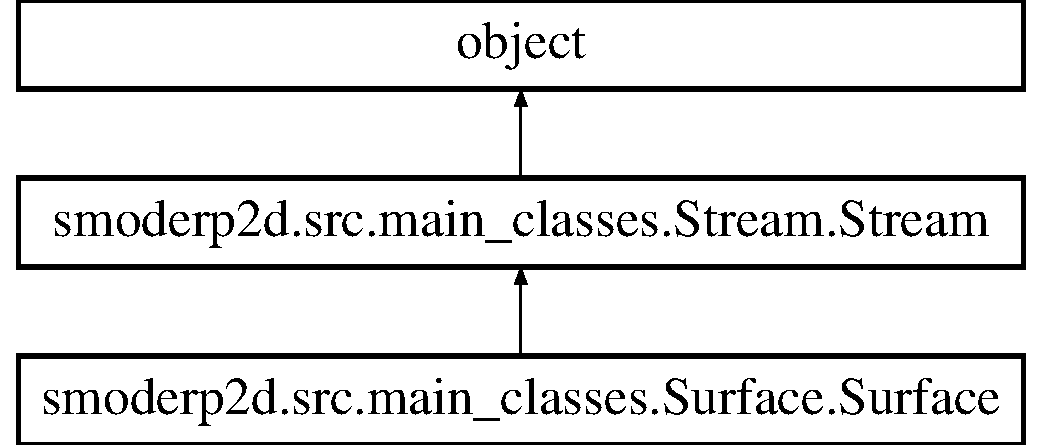
\includegraphics[height=3.000000cm]{d0/d98/classsmoderp2d_1_1src_1_1main__classes_1_1Stream_1_1Stream}
\end{center}
\end{figure}
\subsection*{Public Member Functions}
\begin{DoxyCompactItemize}
\item 
def \hyperlink{classsmoderp2d_1_1src_1_1main__classes_1_1Stream_1_1Stream_ac84e877bd72b3626b2f8ef573b10aa58}{\-\_\-\-\_\-init\-\_\-\-\_\-}
\begin{DoxyCompactList}\small\item\em The constructor. \end{DoxyCompactList}\item 
\hypertarget{classsmoderp2d_1_1src_1_1main__classes_1_1Stream_1_1Stream_a3b32812f8a9ca3ddb0626758fe08a8b0}{def {\bfseries reset\-\_\-inflows}}\label{classsmoderp2d_1_1src_1_1main__classes_1_1Stream_1_1Stream_a3b32812f8a9ca3ddb0626758fe08a8b0}

\item 
def \hyperlink{classsmoderp2d_1_1src_1_1main__classes_1_1Stream_1_1Stream_a1c85299deecf303c9552d8cf93025e88}{reach\-\_\-inflows}
\begin{DoxyCompactList}\small\item\em Documentation for a reach inflows. \end{DoxyCompactList}\item 
\hypertarget{classsmoderp2d_1_1src_1_1main__classes_1_1Stream_1_1Stream_a61da102f7c01c9edee925180bc6ce072}{def {\bfseries stream\-\_\-reach\-\_\-outflow}}\label{classsmoderp2d_1_1src_1_1main__classes_1_1Stream_1_1Stream_a61da102f7c01c9edee925180bc6ce072}

\item 
\hypertarget{classsmoderp2d_1_1src_1_1main__classes_1_1Stream_1_1Stream_aed4214dd9407511c8de3bd154cf25a0d}{def {\bfseries stream\-\_\-reach\-\_\-inflow}}\label{classsmoderp2d_1_1src_1_1main__classes_1_1Stream_1_1Stream_aed4214dd9407511c8de3bd154cf25a0d}

\item 
\hypertarget{classsmoderp2d_1_1src_1_1main__classes_1_1Stream_1_1Stream_ade6a990d820fa0f6373697e4f89ea899}{def {\bfseries stream\-\_\-cumulative}}\label{classsmoderp2d_1_1src_1_1main__classes_1_1Stream_1_1Stream_ade6a990d820fa0f6373697e4f89ea899}

\item 
\hypertarget{classsmoderp2d_1_1src_1_1main__classes_1_1Stream_1_1Stream_ac37afe4a6a2b20001504bf2a06d16289}{def {\bfseries return\-\_\-stream\-\_\-str\-\_\-vals}}\label{classsmoderp2d_1_1src_1_1main__classes_1_1Stream_1_1Stream_ac37afe4a6a2b20001504bf2a06d16289}

\end{DoxyCompactItemize}
\subsection*{Public Attributes}
\begin{DoxyCompactItemize}
\item 
\hypertarget{classsmoderp2d_1_1src_1_1main__classes_1_1Stream_1_1Stream_a4790a4ff2b3d4b64959643abb6095160}{{\bfseries toky}}\label{classsmoderp2d_1_1src_1_1main__classes_1_1Stream_1_1Stream_a4790a4ff2b3d4b64959643abb6095160}

\item 
\hypertarget{classsmoderp2d_1_1src_1_1main__classes_1_1Stream_1_1Stream_a7c5fba7809cfbcc9587cc0497b7b1ee1}{{\bfseries n\-Reaches}}\label{classsmoderp2d_1_1src_1_1main__classes_1_1Stream_1_1Stream_a7c5fba7809cfbcc9587cc0497b7b1ee1}

\item 
\hypertarget{classsmoderp2d_1_1src_1_1main__classes_1_1Stream_1_1Stream_ab220835e68e769cc33ee838ad73f9ea6}{{\bfseries cell\-\_\-stream}}\label{classsmoderp2d_1_1src_1_1main__classes_1_1Stream_1_1Stream_ab220835e68e769cc33ee838ad73f9ea6}

\item 
\hypertarget{classsmoderp2d_1_1src_1_1main__classes_1_1Stream_1_1Stream_a68e0ac6d8700f0b5954ee909e434e48b}{{\bfseries reach}}\label{classsmoderp2d_1_1src_1_1main__classes_1_1Stream_1_1Stream_a68e0ac6d8700f0b5954ee909e434e48b}

\item 
\hypertarget{classsmoderp2d_1_1src_1_1main__classes_1_1Stream_1_1Stream_a7e48f101cff7b3fbaa3e6bb22dd21af7}{{\bfseries toky\-Loc}}\label{classsmoderp2d_1_1src_1_1main__classes_1_1Stream_1_1Stream_a7e48f101cff7b3fbaa3e6bb22dd21af7}

\item 
\hypertarget{classsmoderp2d_1_1src_1_1main__classes_1_1Stream_1_1Stream_a9150d380caea13606e456b966ce1d7fc}{{\bfseries mat\-\_\-tok\-\_\-usek}}\label{classsmoderp2d_1_1src_1_1main__classes_1_1Stream_1_1Stream_a9150d380caea13606e456b966ce1d7fc}

\item 
\hypertarget{classsmoderp2d_1_1src_1_1main__classes_1_1Stream_1_1Stream_ae142c6e8662af37083de5348d9dd8b70}{{\bfseries S\-T\-R\-E\-A\-M\-\_\-\-R\-A\-T\-I\-O}}\label{classsmoderp2d_1_1src_1_1main__classes_1_1Stream_1_1Stream_ae142c6e8662af37083de5348d9dd8b70}

\end{DoxyCompactItemize}


\subsection{Detailed Description}
Documentation for a class. 

More details. 

Definition at line 76 of file Stream.\-py.



\subsection{Constructor \& Destructor Documentation}
\hypertarget{classsmoderp2d_1_1src_1_1main__classes_1_1Stream_1_1Stream_ac84e877bd72b3626b2f8ef573b10aa58}{\index{smoderp2d\-::src\-::main\-\_\-classes\-::\-Stream\-::\-Stream@{smoderp2d\-::src\-::main\-\_\-classes\-::\-Stream\-::\-Stream}!\-\_\-\-\_\-init\-\_\-\-\_\-@{\-\_\-\-\_\-init\-\_\-\-\_\-}}
\index{\-\_\-\-\_\-init\-\_\-\-\_\-@{\-\_\-\-\_\-init\-\_\-\-\_\-}!smoderp2d::src::main_classes::Stream::Stream@{smoderp2d\-::src\-::main\-\_\-classes\-::\-Stream\-::\-Stream}}
\subsubsection[{\-\_\-\-\_\-init\-\_\-\-\_\-}]{\setlength{\rightskip}{0pt plus 5cm}def smoderp2d.\-src.\-main\-\_\-classes.\-Stream.\-Stream.\-\_\-\-\_\-init\-\_\-\-\_\- (
\begin{DoxyParamCaption}
\item[{}]{self}
\end{DoxyParamCaption}
)}}\label{classsmoderp2d_1_1src_1_1main__classes_1_1Stream_1_1Stream_ac84e877bd72b3626b2f8ef573b10aa58}


The constructor. 



Definition at line 79 of file Stream.\-py.


\begin{DoxyCode}
79 
80   \textcolor{keyword}{def }\hyperlink{classsmoderp2d_1_1src_1_1main__classes_1_1Stream_1_1Stream_ac84e877bd72b3626b2f8ef573b10aa58}{\_\_init\_\_}(self):
81     \textcolor{comment}{#jj}
82     prt.message(\textcolor{stringliteral}{'Stream:'})
83     prt.message(\textcolor{stringliteral}{'\(\backslash\)tON'})
84     super(Stream, self).\hyperlink{classsmoderp2d_1_1src_1_1main__classes_1_1Stream_1_1Stream_ac84e877bd72b3626b2f8ef573b10aa58}{\_\_init\_\_}()
85 
86     \textcolor{comment}{# pak kouknout co je treba jen uvnitr tridy}
87     \textcolor{comment}{#self.temp\_dp = sp.temp\_dp}
88 
89     \textcolor{comment}{# listy v poradi 'FID' 'POINT\_X' 'POINT\_Y' 'POINT\_X\_1' 'POINT\_Y\_1' 'to\_node' 'length' 'sklon' 'smoderp'
       'CISLO' 'TVAR' 'B' 'M' 'DRSNOST' 'Q365'}
90     self.\hyperlink{classsmoderp2d_1_1src_1_1main__classes_1_1Stream_1_1Stream_a4790a4ff2b3d4b64959643abb6095160}{toky} = Gl.toky \textcolor{comment}{# tu jsou nactena data z data preparation cca lajna 970}
91 
92     self.\hyperlink{classsmoderp2d_1_1src_1_1main__classes_1_1Stream_1_1Stream_a7c5fba7809cfbcc9587cc0497b7b1ee1}{nReaches} = len(self.\hyperlink{classsmoderp2d_1_1src_1_1main__classes_1_1Stream_1_1Stream_a4790a4ff2b3d4b64959643abb6095160}{toky}[0])
93     
94     
95     self.\hyperlink{classsmoderp2d_1_1src_1_1main__classes_1_1Stream_1_1Stream_ab220835e68e769cc33ee838ad73f9ea6}{cell\_stream} = Gl.cell\_stream
96 
97     self.\hyperlink{classsmoderp2d_1_1src_1_1main__classes_1_1Stream_1_1Stream_a68e0ac6d8700f0b5954ee909e434e48b}{reach} = []
98     
99     \textcolor{keywordflow}{for} i \textcolor{keywordflow}{in} range(self.\hyperlink{classsmoderp2d_1_1src_1_1main__classes_1_1Stream_1_1Stream_a7c5fba7809cfbcc9587cc0497b7b1ee1}{nReaches}):
100       self.reach.append(\hyperlink{classsmoderp2d_1_1src_1_1main__classes_1_1Stream_1_1Reach}{Reach}(self.\hyperlink{classsmoderp2d_1_1src_1_1main__classes_1_1Stream_1_1Stream_a4790a4ff2b3d4b64959643abb6095160}{toky}[0][i],self.\hyperlink{classsmoderp2d_1_1src_1_1main__classes_1_1Stream_1_1Stream_a4790a4ff2b3d4b64959643abb6095160}{toky}[1][i],self.
      \hyperlink{classsmoderp2d_1_1src_1_1main__classes_1_1Stream_1_1Stream_a4790a4ff2b3d4b64959643abb6095160}{toky}[2][i],self.\hyperlink{classsmoderp2d_1_1src_1_1main__classes_1_1Stream_1_1Stream_a4790a4ff2b3d4b64959643abb6095160}{toky}[3][i],self.\hyperlink{classsmoderp2d_1_1src_1_1main__classes_1_1Stream_1_1Stream_a4790a4ff2b3d4b64959643abb6095160}{toky}[4][i],self.\hyperlink{classsmoderp2d_1_1src_1_1main__classes_1_1Stream_1_1Stream_a4790a4ff2b3d4b64959643abb6095160}{toky}[5][i],self.
      \hyperlink{classsmoderp2d_1_1src_1_1main__classes_1_1Stream_1_1Stream_a4790a4ff2b3d4b64959643abb6095160}{toky}[6][i],self.\hyperlink{classsmoderp2d_1_1src_1_1main__classes_1_1Stream_1_1Stream_a4790a4ff2b3d4b64959643abb6095160}{toky}[7][i],self.\hyperlink{classsmoderp2d_1_1src_1_1main__classes_1_1Stream_1_1Stream_a4790a4ff2b3d4b64959643abb6095160}{toky}[8][i],self.\hyperlink{classsmoderp2d_1_1src_1_1main__classes_1_1Stream_1_1Stream_a4790a4ff2b3d4b64959643abb6095160}{toky}[9][i],self.
      \hyperlink{classsmoderp2d_1_1src_1_1main__classes_1_1Stream_1_1Stream_a4790a4ff2b3d4b64959643abb6095160}{toky}[10][i],self.\hyperlink{classsmoderp2d_1_1src_1_1main__classes_1_1Stream_1_1Stream_a4790a4ff2b3d4b64959643abb6095160}{toky}[11][i],self.\hyperlink{classsmoderp2d_1_1src_1_1main__classes_1_1Stream_1_1Stream_a4790a4ff2b3d4b64959643abb6095160}{toky}[12][i],self.\hyperlink{classsmoderp2d_1_1src_1_1main__classes_1_1Stream_1_1Stream_a4790a4ff2b3d4b64959643abb6095160}{toky}[13][i],self.
      \hyperlink{classsmoderp2d_1_1src_1_1main__classes_1_1Stream_1_1Stream_a4790a4ff2b3d4b64959643abb6095160}{toky}[14][i]))
101 
102     self.\hyperlink{classsmoderp2d_1_1src_1_1main__classes_1_1Stream_1_1Stream_a7e48f101cff7b3fbaa3e6bb22dd21af7}{tokyLoc}      = Gl.tokyLoc
103     self.\hyperlink{classsmoderp2d_1_1src_1_1main__classes_1_1Stream_1_1Stream_a9150d380caea13606e456b966ce1d7fc}{mat\_tok\_usek} = Gl.mat\_tok\_usek
104     
105     
106 
107     
108     \textcolor{keywordflow}{for} i \textcolor{keywordflow}{in} Gl.rr :
109       \textcolor{keywordflow}{for} j \textcolor{keywordflow}{in} Gl.rc[i]:
110         self.arr[i][j].state += self.\hyperlink{classsmoderp2d_1_1src_1_1main__classes_1_1Stream_1_1Stream_a9150d380caea13606e456b966ce1d7fc}{mat\_tok\_usek}[i][j]
111 
112     self.\hyperlink{classsmoderp2d_1_1src_1_1main__classes_1_1Stream_1_1Stream_ae142c6e8662af37083de5348d9dd8b70}{STREAM\_RATIO} = Gl.STREAM\_RATIO
113 

\end{DoxyCode}


\subsection{Member Function Documentation}
\hypertarget{classsmoderp2d_1_1src_1_1main__classes_1_1Stream_1_1Stream_a1c85299deecf303c9552d8cf93025e88}{\index{smoderp2d\-::src\-::main\-\_\-classes\-::\-Stream\-::\-Stream@{smoderp2d\-::src\-::main\-\_\-classes\-::\-Stream\-::\-Stream}!reach\-\_\-inflows@{reach\-\_\-inflows}}
\index{reach\-\_\-inflows@{reach\-\_\-inflows}!smoderp2d::src::main_classes::Stream::Stream@{smoderp2d\-::src\-::main\-\_\-classes\-::\-Stream\-::\-Stream}}
\subsubsection[{reach\-\_\-inflows}]{\setlength{\rightskip}{0pt plus 5cm}def smoderp2d.\-src.\-main\-\_\-classes.\-Stream.\-Stream.\-reach\-\_\-inflows (
\begin{DoxyParamCaption}
\item[{}]{self, }
\item[{}]{id\-\_\-, }
\item[{}]{inflows}
\end{DoxyParamCaption}
)}}\label{classsmoderp2d_1_1src_1_1main__classes_1_1Stream_1_1Stream_a1c85299deecf303c9552d8cf93025e88}


Documentation for a reach inflows. 


\begin{DoxyParams}{Parameters}
{\em id\-\_\-} & starts in 0 not 1000 \\
\hline
\end{DoxyParams}


Definition at line 121 of file Stream.\-py.


\begin{DoxyCode}
121 
122   \textcolor{keyword}{def }\hyperlink{classsmoderp2d_1_1src_1_1main__classes_1_1Stream_1_1Stream_a1c85299deecf303c9552d8cf93025e88}{reach\_inflows}(self,id\_, inflows):
123     self.\hyperlink{classsmoderp2d_1_1src_1_1main__classes_1_1Stream_1_1Stream_a68e0ac6d8700f0b5954ee909e434e48b}{reach}[id\_].V\_in\_from\_field += inflows

\end{DoxyCode}


The documentation for this class was generated from the following file\-:\begin{DoxyCompactItemize}
\item 
smoderp2d/src/main\-\_\-classes/Stream.\-py\end{DoxyCompactItemize}

\hypertarget{classsmoderp2d_1_1src_1_1main__classes_1_1Stream_1_1StreamPass}{\section{smoderp2d.\-src.\-main\-\_\-classes.\-Stream.\-Stream\-Pass Class Reference}
\label{classsmoderp2d_1_1src_1_1main__classes_1_1Stream_1_1StreamPass}\index{smoderp2d.\-src.\-main\-\_\-classes.\-Stream.\-Stream\-Pass@{smoderp2d.\-src.\-main\-\_\-classes.\-Stream.\-Stream\-Pass}}
}
Inheritance diagram for smoderp2d.\-src.\-main\-\_\-classes.\-Stream.\-Stream\-Pass\-:\begin{figure}[H]
\begin{center}
\leavevmode
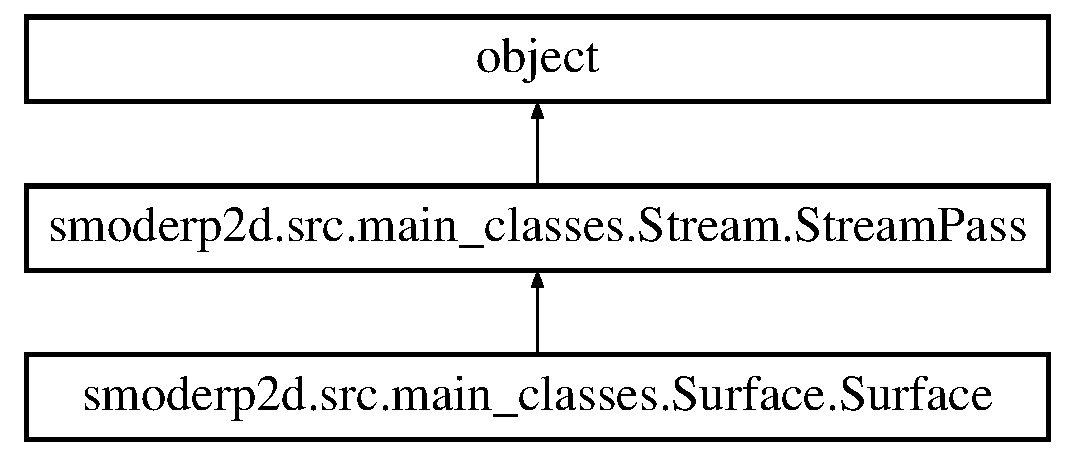
\includegraphics[height=3.000000cm]{classsmoderp2d_1_1src_1_1main__classes_1_1Stream_1_1StreamPass}
\end{center}
\end{figure}
\subsection*{Public Member Functions}
\begin{DoxyCompactItemize}
\item 
\hypertarget{classsmoderp2d_1_1src_1_1main__classes_1_1Stream_1_1StreamPass_a104c4216b1d7131b0eab1f8c16918b79}{def {\bfseries \-\_\-\-\_\-init\-\_\-\-\_\-}}\label{classsmoderp2d_1_1src_1_1main__classes_1_1Stream_1_1StreamPass_a104c4216b1d7131b0eab1f8c16918b79}

\item 
\hypertarget{classsmoderp2d_1_1src_1_1main__classes_1_1Stream_1_1StreamPass_a79fe170e436e449eb6741ad7de78d4fe}{def {\bfseries reset\-\_\-inflows}}\label{classsmoderp2d_1_1src_1_1main__classes_1_1Stream_1_1StreamPass_a79fe170e436e449eb6741ad7de78d4fe}

\item 
\hypertarget{classsmoderp2d_1_1src_1_1main__classes_1_1Stream_1_1StreamPass_a6a3307d529c06df9d0be7d08d663fcac}{def {\bfseries reach\-\_\-inflows}}\label{classsmoderp2d_1_1src_1_1main__classes_1_1Stream_1_1StreamPass_a6a3307d529c06df9d0be7d08d663fcac}

\item 
\hypertarget{classsmoderp2d_1_1src_1_1main__classes_1_1Stream_1_1StreamPass_ab936214091b6251d511615d6144db0b2}{def {\bfseries stream\-\_\-reach\-\_\-inflow}}\label{classsmoderp2d_1_1src_1_1main__classes_1_1Stream_1_1StreamPass_ab936214091b6251d511615d6144db0b2}

\item 
\hypertarget{classsmoderp2d_1_1src_1_1main__classes_1_1Stream_1_1StreamPass_a15968039ec33a1f47b908f2cb0357524}{def {\bfseries stream\-\_\-reach\-\_\-outflow}}\label{classsmoderp2d_1_1src_1_1main__classes_1_1Stream_1_1StreamPass_a15968039ec33a1f47b908f2cb0357524}

\item 
\hypertarget{classsmoderp2d_1_1src_1_1main__classes_1_1Stream_1_1StreamPass_a1a2803c1bd7824c0fcf3d356690d2d29}{def {\bfseries stream\-\_\-cumulative}}\label{classsmoderp2d_1_1src_1_1main__classes_1_1Stream_1_1StreamPass_a1a2803c1bd7824c0fcf3d356690d2d29}

\end{DoxyCompactItemize}


The documentation for this class was generated from the following file\-:\begin{DoxyCompactItemize}
\item 
smoderp2d/src/main\-\_\-classes/Stream.\-py\end{DoxyCompactItemize}

\hypertarget{classsmoderp2d_1_1src_1_1main__classes_1_1Subsurface_1_1SubArrs}{\section{smoderp2d.\-src.\-main\-\_\-classes.\-Subsurface.\-Sub\-Arrs Class Reference}
\label{classsmoderp2d_1_1src_1_1main__classes_1_1Subsurface_1_1SubArrs}\index{smoderp2d.\-src.\-main\-\_\-classes.\-Subsurface.\-Sub\-Arrs@{smoderp2d.\-src.\-main\-\_\-classes.\-Subsurface.\-Sub\-Arrs}}
}
\subsection*{Public Member Functions}
\begin{DoxyCompactItemize}
\item 
\hypertarget{classsmoderp2d_1_1src_1_1main__classes_1_1Subsurface_1_1SubArrs_a469869c54f5c187426f403c6ce1ce878}{def {\bfseries \-\_\-\-\_\-init\-\_\-\-\_\-}}\label{classsmoderp2d_1_1src_1_1main__classes_1_1Subsurface_1_1SubArrs_a469869c54f5c187426f403c6ce1ce878}

\end{DoxyCompactItemize}
\subsection*{Public Attributes}
\begin{DoxyCompactItemize}
\item 
\hypertarget{classsmoderp2d_1_1src_1_1main__classes_1_1Subsurface_1_1SubArrs_ad39e09e33f5da84184ff473e58fe5e49}{{\bfseries L\-\_\-sub}}\label{classsmoderp2d_1_1src_1_1main__classes_1_1Subsurface_1_1SubArrs_ad39e09e33f5da84184ff473e58fe5e49}

\item 
\hypertarget{classsmoderp2d_1_1src_1_1main__classes_1_1Subsurface_1_1SubArrs_a73dcbb43f879793a5ad7014b10215ecc}{{\bfseries h}}\label{classsmoderp2d_1_1src_1_1main__classes_1_1Subsurface_1_1SubArrs_a73dcbb43f879793a5ad7014b10215ecc}

\item 
\hypertarget{classsmoderp2d_1_1src_1_1main__classes_1_1Subsurface_1_1SubArrs_a5c97d30acbf4327c10642104b8304555}{{\bfseries H}}\label{classsmoderp2d_1_1src_1_1main__classes_1_1Subsurface_1_1SubArrs_a5c97d30acbf4327c10642104b8304555}

\item 
\hypertarget{classsmoderp2d_1_1src_1_1main__classes_1_1Subsurface_1_1SubArrs_a16c4ec53a69baa7b37b8492b5ec11a46}{{\bfseries z}}\label{classsmoderp2d_1_1src_1_1main__classes_1_1Subsurface_1_1SubArrs_a16c4ec53a69baa7b37b8492b5ec11a46}

\item 
\hypertarget{classsmoderp2d_1_1src_1_1main__classes_1_1Subsurface_1_1SubArrs_a69ff54bd2f6aa4c54654e709488f119d}{{\bfseries slope}}\label{classsmoderp2d_1_1src_1_1main__classes_1_1Subsurface_1_1SubArrs_a69ff54bd2f6aa4c54654e709488f119d}

\item 
\hypertarget{classsmoderp2d_1_1src_1_1main__classes_1_1Subsurface_1_1SubArrs_ac721f9634533010f5d627507b2dcc3f9}{{\bfseries exfiltration}}\label{classsmoderp2d_1_1src_1_1main__classes_1_1Subsurface_1_1SubArrs_ac721f9634533010f5d627507b2dcc3f9}

\item 
\hypertarget{classsmoderp2d_1_1src_1_1main__classes_1_1Subsurface_1_1SubArrs_a47bdea640a977a137261a1cf3dcca167}{{\bfseries V\-\_\-runoff}}\label{classsmoderp2d_1_1src_1_1main__classes_1_1Subsurface_1_1SubArrs_a47bdea640a977a137261a1cf3dcca167}

\item 
\hypertarget{classsmoderp2d_1_1src_1_1main__classes_1_1Subsurface_1_1SubArrs_a29f664c5df61a15bda82279f12825bb6}{{\bfseries V\-\_\-runoff\-\_\-pre}}\label{classsmoderp2d_1_1src_1_1main__classes_1_1Subsurface_1_1SubArrs_a29f664c5df61a15bda82279f12825bb6}

\item 
\hypertarget{classsmoderp2d_1_1src_1_1main__classes_1_1Subsurface_1_1SubArrs_a691bef39cf51da5efdb94fea1f2272a1}{{\bfseries V\-\_\-rest}}\label{classsmoderp2d_1_1src_1_1main__classes_1_1Subsurface_1_1SubArrs_a691bef39cf51da5efdb94fea1f2272a1}

\item 
\hypertarget{classsmoderp2d_1_1src_1_1main__classes_1_1Subsurface_1_1SubArrs_a28d30e4ccd34097521288936adc91529}{{\bfseries Ks}}\label{classsmoderp2d_1_1src_1_1main__classes_1_1Subsurface_1_1SubArrs_a28d30e4ccd34097521288936adc91529}

\item 
\hypertarget{classsmoderp2d_1_1src_1_1main__classes_1_1Subsurface_1_1SubArrs_a87b6c5d67b9fac775260fd7a844fc9b3}{{\bfseries cum\-\_\-percolation}}\label{classsmoderp2d_1_1src_1_1main__classes_1_1Subsurface_1_1SubArrs_a87b6c5d67b9fac775260fd7a844fc9b3}

\item 
\hypertarget{classsmoderp2d_1_1src_1_1main__classes_1_1Subsurface_1_1SubArrs_a65c22873728ec0970ca12b93693eaa03}{{\bfseries percolation}}\label{classsmoderp2d_1_1src_1_1main__classes_1_1Subsurface_1_1SubArrs_a65c22873728ec0970ca12b93693eaa03}

\item 
\hypertarget{classsmoderp2d_1_1src_1_1main__classes_1_1Subsurface_1_1SubArrs_a20b6c1f5d889d73c51edb0478822eeca}{{\bfseries vg\-\_\-n}}\label{classsmoderp2d_1_1src_1_1main__classes_1_1Subsurface_1_1SubArrs_a20b6c1f5d889d73c51edb0478822eeca}

\item 
\hypertarget{classsmoderp2d_1_1src_1_1main__classes_1_1Subsurface_1_1SubArrs_afa2076afdd18d58dc43a0172345d2c15}{{\bfseries vg\-\_\-m}}\label{classsmoderp2d_1_1src_1_1main__classes_1_1Subsurface_1_1SubArrs_afa2076afdd18d58dc43a0172345d2c15}

\item 
\hypertarget{classsmoderp2d_1_1src_1_1main__classes_1_1Subsurface_1_1SubArrs_adb7cbc36ecc6a600feaad990a1769645}{{\bfseries vg\-\_\-l}}\label{classsmoderp2d_1_1src_1_1main__classes_1_1Subsurface_1_1SubArrs_adb7cbc36ecc6a600feaad990a1769645}

\end{DoxyCompactItemize}


The documentation for this class was generated from the following file\-:\begin{DoxyCompactItemize}
\item 
smoderp2d/src/main\-\_\-classes/Subsurface.\-py\end{DoxyCompactItemize}

\hypertarget{classsmoderp2d_1_1src_1_1main__classes_1_1Subsurface_1_1Subsurface}{\section{smoderp2d.\-src.\-main\-\_\-classes.\-Subsurface.\-Subsurface Class Reference}
\label{classsmoderp2d_1_1src_1_1main__classes_1_1Subsurface_1_1Subsurface}\index{smoderp2d.\-src.\-main\-\_\-classes.\-Subsurface.\-Subsurface@{smoderp2d.\-src.\-main\-\_\-classes.\-Subsurface.\-Subsurface}}
}
Inheritance diagram for smoderp2d.\-src.\-main\-\_\-classes.\-Subsurface.\-Subsurface\-:\begin{figure}[H]
\begin{center}
\leavevmode
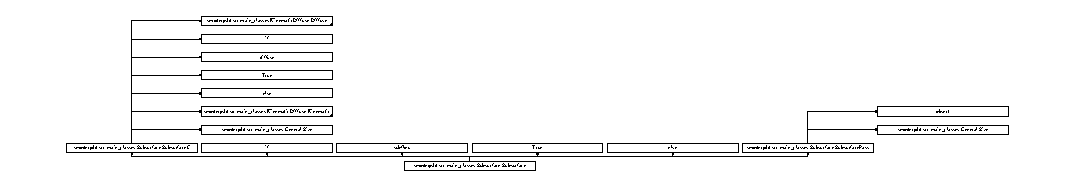
\includegraphics[height=2.068965cm]{d9/df4/classsmoderp2d_1_1src_1_1main__classes_1_1Subsurface_1_1Subsurface}
\end{center}
\end{figure}
\subsection*{Public Member Functions}
\begin{DoxyCompactItemize}
\item 
\hypertarget{classsmoderp2d_1_1src_1_1main__classes_1_1Subsurface_1_1Subsurface_a64abac9f92b883482bdeba247c6b5d44}{def {\bfseries \-\_\-\-\_\-init\-\_\-\-\_\-}}\label{classsmoderp2d_1_1src_1_1main__classes_1_1Subsurface_1_1Subsurface_a64abac9f92b883482bdeba247c6b5d44}

\end{DoxyCompactItemize}
\subsection*{Additional Inherited Members}


\subsection{Detailed Description}


Definition at line 192 of file Subsurface.\-py.



The documentation for this class was generated from the following file\-:\begin{DoxyCompactItemize}
\item 
smoderp2d/src/main\-\_\-classes/Subsurface.\-py\end{DoxyCompactItemize}

\hypertarget{classsmoderp2d_1_1src_1_1main__classes_1_1Subsurface_1_1SubsurfaceC}{\section{smoderp2d.\-src.\-main\-\_\-classes.\-Subsurface.\-Subsurface\-C Class Reference}
\label{classsmoderp2d_1_1src_1_1main__classes_1_1Subsurface_1_1SubsurfaceC}\index{smoderp2d.\-src.\-main\-\_\-classes.\-Subsurface.\-Subsurface\-C@{smoderp2d.\-src.\-main\-\_\-classes.\-Subsurface.\-Subsurface\-C}}
}


Documentation for a class.  


Inheritance diagram for smoderp2d.\-src.\-main\-\_\-classes.\-Subsurface.\-Subsurface\-C\-:\begin{figure}[H]
\begin{center}
\leavevmode
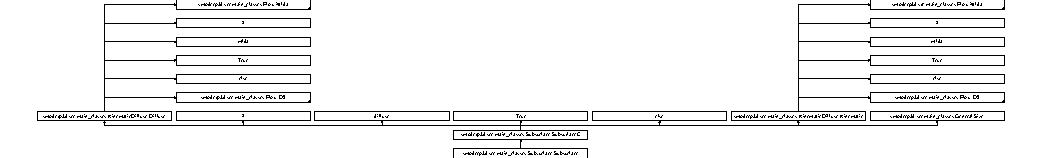
\includegraphics[height=2.123894cm]{classsmoderp2d_1_1src_1_1main__classes_1_1Subsurface_1_1SubsurfaceC}
\end{center}
\end{figure}
\subsection*{Public Member Functions}
\begin{DoxyCompactItemize}
\item 
\hypertarget{classsmoderp2d_1_1src_1_1main__classes_1_1Subsurface_1_1SubsurfaceC_ada42aeb92c152e1ef808ed85aef76881}{def {\bfseries \-\_\-\-\_\-init\-\_\-\-\_\-}}\label{classsmoderp2d_1_1src_1_1main__classes_1_1Subsurface_1_1SubsurfaceC_ada42aeb92c152e1ef808ed85aef76881}

\item 
\hypertarget{classsmoderp2d_1_1src_1_1main__classes_1_1Subsurface_1_1SubsurfaceC_a08029ffd054df335ec98ce0b49cb1c42}{def {\bfseries slope\-\_\-}}\label{classsmoderp2d_1_1src_1_1main__classes_1_1Subsurface_1_1SubsurfaceC_a08029ffd054df335ec98ce0b49cb1c42}

\item 
\hypertarget{classsmoderp2d_1_1src_1_1main__classes_1_1Subsurface_1_1SubsurfaceC_a24c4c8f0f043f540b7ec851c7be5bcbd}{def {\bfseries fill\-\_\-slope}}\label{classsmoderp2d_1_1src_1_1main__classes_1_1Subsurface_1_1SubsurfaceC_a24c4c8f0f043f540b7ec851c7be5bcbd}

\item 
\hypertarget{classsmoderp2d_1_1src_1_1main__classes_1_1Subsurface_1_1SubsurfaceC_add45657622029774bb4f6f3122f646b4}{def {\bfseries get\-\_\-exfiltration}}\label{classsmoderp2d_1_1src_1_1main__classes_1_1Subsurface_1_1SubsurfaceC_add45657622029774bb4f6f3122f646b4}

\item 
\hypertarget{classsmoderp2d_1_1src_1_1main__classes_1_1Subsurface_1_1SubsurfaceC_a58faea7825ecf1fb6f61631912612a98}{def {\bfseries bilance}}\label{classsmoderp2d_1_1src_1_1main__classes_1_1Subsurface_1_1SubsurfaceC_a58faea7825ecf1fb6f61631912612a98}

\item 
\hypertarget{classsmoderp2d_1_1src_1_1main__classes_1_1Subsurface_1_1SubsurfaceC_a18794c9dd9ff301aecfc3a12312c4509}{def {\bfseries calc\-\_\-percolation}}\label{classsmoderp2d_1_1src_1_1main__classes_1_1Subsurface_1_1SubsurfaceC_a18794c9dd9ff301aecfc3a12312c4509}

\item 
\hypertarget{classsmoderp2d_1_1src_1_1main__classes_1_1Subsurface_1_1SubsurfaceC_ae0089360bb2eba3578b42a1fbdc48b73}{def {\bfseries calc\-\_\-exfiltration}}\label{classsmoderp2d_1_1src_1_1main__classes_1_1Subsurface_1_1SubsurfaceC_ae0089360bb2eba3578b42a1fbdc48b73}

\item 
\hypertarget{classsmoderp2d_1_1src_1_1main__classes_1_1Subsurface_1_1SubsurfaceC_a70c5e1576bc926fd6722312e86743e81}{def {\bfseries runoff}}\label{classsmoderp2d_1_1src_1_1main__classes_1_1Subsurface_1_1SubsurfaceC_a70c5e1576bc926fd6722312e86743e81}

\item 
\hypertarget{classsmoderp2d_1_1src_1_1main__classes_1_1Subsurface_1_1SubsurfaceC_ac1b5abd564da9ce667c8f124593db6b2}{def {\bfseries runoff\-\_\-stream\-\_\-cell}}\label{classsmoderp2d_1_1src_1_1main__classes_1_1Subsurface_1_1SubsurfaceC_ac1b5abd564da9ce667c8f124593db6b2}

\item 
\hypertarget{classsmoderp2d_1_1src_1_1main__classes_1_1Subsurface_1_1SubsurfaceC_a0536bb2dc32f8a25c3925c1c00ed765f}{def {\bfseries curr\-\_\-to\-\_\-pre}}\label{classsmoderp2d_1_1src_1_1main__classes_1_1Subsurface_1_1SubsurfaceC_a0536bb2dc32f8a25c3925c1c00ed765f}

\item 
\hypertarget{classsmoderp2d_1_1src_1_1main__classes_1_1Subsurface_1_1SubsurfaceC_a21dec1099ac14167aa3ef5e188fb8158}{def {\bfseries return\-\_\-str\-\_\-vals}}\label{classsmoderp2d_1_1src_1_1main__classes_1_1Subsurface_1_1SubsurfaceC_a21dec1099ac14167aa3ef5e188fb8158}

\end{DoxyCompactItemize}
\subsection*{Public Attributes}
\begin{DoxyCompactItemize}
\item 
\hypertarget{classsmoderp2d_1_1src_1_1main__classes_1_1Subsurface_1_1SubsurfaceC_ad7df6915d0cdc23d446f9bb0ef70593c}{{\bfseries arr}}\label{classsmoderp2d_1_1src_1_1main__classes_1_1Subsurface_1_1SubsurfaceC_ad7df6915d0cdc23d446f9bb0ef70593c}

\item 
\hypertarget{classsmoderp2d_1_1src_1_1main__classes_1_1Subsurface_1_1SubsurfaceC_ae39da2fc8db1e3ceafd99c917a06b33c}{{\bfseries Kr}}\label{classsmoderp2d_1_1src_1_1main__classes_1_1Subsurface_1_1SubsurfaceC_ae39da2fc8db1e3ceafd99c917a06b33c}

\item 
\hypertarget{classsmoderp2d_1_1src_1_1main__classes_1_1Subsurface_1_1SubsurfaceC_a8bbe35472749dba7e9d9695272e0130c}{{\bfseries darcy}}\label{classsmoderp2d_1_1src_1_1main__classes_1_1Subsurface_1_1SubsurfaceC_a8bbe35472749dba7e9d9695272e0130c}

\item 
\hypertarget{classsmoderp2d_1_1src_1_1main__classes_1_1Subsurface_1_1SubsurfaceC_a061ba89ce915a308ba9f955f3fec65e1}{{\bfseries q\-\_\-subsurface}}\label{classsmoderp2d_1_1src_1_1main__classes_1_1Subsurface_1_1SubsurfaceC_a061ba89ce915a308ba9f955f3fec65e1}

\end{DoxyCompactItemize}


\subsection{Detailed Description}
Documentation for a class. 

More details. 

The documentation for this class was generated from the following file\-:\begin{DoxyCompactItemize}
\item 
smoderp2d/src/main\-\_\-classes/Subsurface.\-py\end{DoxyCompactItemize}

\hypertarget{classsmoderp2d_1_1src_1_1main__classes_1_1Subsurface_1_1SubsurfacePass}{\section{smoderp2d.\-src.\-main\-\_\-classes.\-Subsurface.\-Subsurface\-Pass Class Reference}
\label{classsmoderp2d_1_1src_1_1main__classes_1_1Subsurface_1_1SubsurfacePass}\index{smoderp2d.\-src.\-main\-\_\-classes.\-Subsurface.\-Subsurface\-Pass@{smoderp2d.\-src.\-main\-\_\-classes.\-Subsurface.\-Subsurface\-Pass}}
}


Class empty class if no subsurface flow is considered.  


Inheritance diagram for smoderp2d.\-src.\-main\-\_\-classes.\-Subsurface.\-Subsurface\-Pass\-:\begin{figure}[H]
\begin{center}
\leavevmode
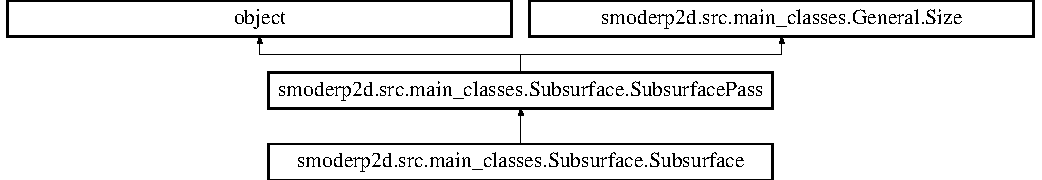
\includegraphics[height=2.413793cm]{d9/d6d/classsmoderp2d_1_1src_1_1main__classes_1_1Subsurface_1_1SubsurfacePass}
\end{center}
\end{figure}
\subsection*{Public Member Functions}
\begin{DoxyCompactItemize}
\item 
\hypertarget{classsmoderp2d_1_1src_1_1main__classes_1_1Subsurface_1_1SubsurfacePass_a2b9ecba613efbd724b8646bb2cf35340}{def {\bfseries \-\_\-\-\_\-init\-\_\-\-\_\-}}\label{classsmoderp2d_1_1src_1_1main__classes_1_1Subsurface_1_1SubsurfacePass_a2b9ecba613efbd724b8646bb2cf35340}

\item 
\hypertarget{classsmoderp2d_1_1src_1_1main__classes_1_1Subsurface_1_1SubsurfacePass_ae616cefffb4308ee893ff310ee2b90df}{def {\bfseries new\-\_\-inflows}}\label{classsmoderp2d_1_1src_1_1main__classes_1_1Subsurface_1_1SubsurfacePass_ae616cefffb4308ee893ff310ee2b90df}

\item 
\hypertarget{classsmoderp2d_1_1src_1_1main__classes_1_1Subsurface_1_1SubsurfacePass_a0a3f7ce3b2dba6b16be1bb1b685c7d5f}{def {\bfseries cell\-\_\-runoff}}\label{classsmoderp2d_1_1src_1_1main__classes_1_1Subsurface_1_1SubsurfacePass_a0a3f7ce3b2dba6b16be1bb1b685c7d5f}

\item 
\hypertarget{classsmoderp2d_1_1src_1_1main__classes_1_1Subsurface_1_1SubsurfacePass_af3cbfbc888097e7a1c2548bb2a5701e3}{def {\bfseries fill\-\_\-slope}}\label{classsmoderp2d_1_1src_1_1main__classes_1_1Subsurface_1_1SubsurfacePass_af3cbfbc888097e7a1c2548bb2a5701e3}

\item 
\hypertarget{classsmoderp2d_1_1src_1_1main__classes_1_1Subsurface_1_1SubsurfacePass_a9b1233261cffd0a8dd5294c9504e65bd}{def {\bfseries get\-\_\-exfiltration}}\label{classsmoderp2d_1_1src_1_1main__classes_1_1Subsurface_1_1SubsurfacePass_a9b1233261cffd0a8dd5294c9504e65bd}

\item 
\hypertarget{classsmoderp2d_1_1src_1_1main__classes_1_1Subsurface_1_1SubsurfacePass_a1088579fad42f09b659d7b4d0211f90c}{def {\bfseries bilance}}\label{classsmoderp2d_1_1src_1_1main__classes_1_1Subsurface_1_1SubsurfacePass_a1088579fad42f09b659d7b4d0211f90c}

\item 
\hypertarget{classsmoderp2d_1_1src_1_1main__classes_1_1Subsurface_1_1SubsurfacePass_a633e45ef168384a8e07e272bca3f98d9}{def {\bfseries runoff}}\label{classsmoderp2d_1_1src_1_1main__classes_1_1Subsurface_1_1SubsurfacePass_a633e45ef168384a8e07e272bca3f98d9}

\item 
\hypertarget{classsmoderp2d_1_1src_1_1main__classes_1_1Subsurface_1_1SubsurfacePass_a154be8d42dd279cf533545c7128697f0}{def {\bfseries runoff\-\_\-stream\-\_\-cell}}\label{classsmoderp2d_1_1src_1_1main__classes_1_1Subsurface_1_1SubsurfacePass_a154be8d42dd279cf533545c7128697f0}

\item 
\hypertarget{classsmoderp2d_1_1src_1_1main__classes_1_1Subsurface_1_1SubsurfacePass_aa803af6a9d76025033b00c980bf36961}{def {\bfseries return\-\_\-str\-\_\-vals}}\label{classsmoderp2d_1_1src_1_1main__classes_1_1Subsurface_1_1SubsurfacePass_aa803af6a9d76025033b00c980bf36961}

\item 
\hypertarget{classsmoderp2d_1_1src_1_1main__classes_1_1Subsurface_1_1SubsurfacePass_a061840e5785c980cde76b41a208792f9}{def {\bfseries curr\-\_\-to\-\_\-pre}}\label{classsmoderp2d_1_1src_1_1main__classes_1_1Subsurface_1_1SubsurfacePass_a061840e5785c980cde76b41a208792f9}

\end{DoxyCompactItemize}
\subsection*{Public Attributes}
\begin{DoxyCompactItemize}
\item 
\hypertarget{classsmoderp2d_1_1src_1_1main__classes_1_1Subsurface_1_1SubsurfacePass_a4e23f0e451462cff2809755e9fb5a9be}{{\bfseries n}}\label{classsmoderp2d_1_1src_1_1main__classes_1_1Subsurface_1_1SubsurfacePass_a4e23f0e451462cff2809755e9fb5a9be}

\item 
\hypertarget{classsmoderp2d_1_1src_1_1main__classes_1_1Subsurface_1_1SubsurfacePass_a821e396c68937e815cbc43b2bd14aaa9}{{\bfseries arr}}\label{classsmoderp2d_1_1src_1_1main__classes_1_1Subsurface_1_1SubsurfacePass_a821e396c68937e815cbc43b2bd14aaa9}

\item 
\hypertarget{classsmoderp2d_1_1src_1_1main__classes_1_1Subsurface_1_1SubsurfacePass_a014d041b86aea9a92b5d1bb46003234f}{{\bfseries q\-\_\-subsurface}}\label{classsmoderp2d_1_1src_1_1main__classes_1_1Subsurface_1_1SubsurfacePass_a014d041b86aea9a92b5d1bb46003234f}

\end{DoxyCompactItemize}


\subsection{Detailed Description}
Class empty class if no subsurface flow is considered. 

Definition at line 163 of file Subsurface.\-py.



The documentation for this class was generated from the following file\-:\begin{DoxyCompactItemize}
\item 
smoderp2d/src/main\-\_\-classes/Subsurface.\-py\end{DoxyCompactItemize}

\hypertarget{classsmoderp2d_1_1src_1_1main__classes_1_1Surface_1_1SurArrs}{\section{smoderp2d.\-src.\-main\-\_\-classes.\-Surface.\-Sur\-Arrs Class Reference}
\label{classsmoderp2d_1_1src_1_1main__classes_1_1Surface_1_1SurArrs}\index{smoderp2d.\-src.\-main\-\_\-classes.\-Surface.\-Sur\-Arrs@{smoderp2d.\-src.\-main\-\_\-classes.\-Surface.\-Sur\-Arrs}}
}
\subsection*{Public Member Functions}
\begin{DoxyCompactItemize}
\item 
\hypertarget{classsmoderp2d_1_1src_1_1main__classes_1_1Surface_1_1SurArrs_a6e477bb70aa8e6c937cb486a1c2b1ce8}{def {\bfseries \-\_\-\-\_\-init\-\_\-\-\_\-}}\label{classsmoderp2d_1_1src_1_1main__classes_1_1Surface_1_1SurArrs_a6e477bb70aa8e6c937cb486a1c2b1ce8}

\end{DoxyCompactItemize}
\subsection*{Public Attributes}
\begin{DoxyCompactItemize}
\item 
\hypertarget{classsmoderp2d_1_1src_1_1main__classes_1_1Surface_1_1SurArrs_a9ecf067b405298db5dc362fb1ca068e1}{{\bfseries state}}\label{classsmoderp2d_1_1src_1_1main__classes_1_1Surface_1_1SurArrs_a9ecf067b405298db5dc362fb1ca068e1}

\item 
\hypertarget{classsmoderp2d_1_1src_1_1main__classes_1_1Surface_1_1SurArrs_ab0b7cc77f4e5bbecc5507bc47b6d3a8b}{{\bfseries sur\-\_\-ret}}\label{classsmoderp2d_1_1src_1_1main__classes_1_1Surface_1_1SurArrs_ab0b7cc77f4e5bbecc5507bc47b6d3a8b}

\item 
\hypertarget{classsmoderp2d_1_1src_1_1main__classes_1_1Surface_1_1SurArrs_a48b7293f778f527fbb5c20b64905bd06}{{\bfseries cur\-\_\-sur\-\_\-ret}}\label{classsmoderp2d_1_1src_1_1main__classes_1_1Surface_1_1SurArrs_a48b7293f778f527fbb5c20b64905bd06}

\item 
\hypertarget{classsmoderp2d_1_1src_1_1main__classes_1_1Surface_1_1SurArrs_aca01b0fe32ef142c217d6bcbb3508959}{{\bfseries cur\-\_\-rain}}\label{classsmoderp2d_1_1src_1_1main__classes_1_1Surface_1_1SurArrs_aca01b0fe32ef142c217d6bcbb3508959}

\item 
\hypertarget{classsmoderp2d_1_1src_1_1main__classes_1_1Surface_1_1SurArrs_a87690226f9f543ff703629145c6559c2}{{\bfseries h\-\_\-sheet}}\label{classsmoderp2d_1_1src_1_1main__classes_1_1Surface_1_1SurArrs_a87690226f9f543ff703629145c6559c2}

\item 
\hypertarget{classsmoderp2d_1_1src_1_1main__classes_1_1Surface_1_1SurArrs_ac9d74c061c2a6be96b9e6069462dee0b}{{\bfseries h\-\_\-total\-\_\-new}}\label{classsmoderp2d_1_1src_1_1main__classes_1_1Surface_1_1SurArrs_ac9d74c061c2a6be96b9e6069462dee0b}

\item 
\hypertarget{classsmoderp2d_1_1src_1_1main__classes_1_1Surface_1_1SurArrs_a202de980fcf095724d576687416cf8da}{{\bfseries h\-\_\-total\-\_\-pre}}\label{classsmoderp2d_1_1src_1_1main__classes_1_1Surface_1_1SurArrs_a202de980fcf095724d576687416cf8da}

\item 
\hypertarget{classsmoderp2d_1_1src_1_1main__classes_1_1Surface_1_1SurArrs_abc374dedd8dfb195d855ba4ac87c5e9a}{{\bfseries V\-\_\-runoff}}\label{classsmoderp2d_1_1src_1_1main__classes_1_1Surface_1_1SurArrs_abc374dedd8dfb195d855ba4ac87c5e9a}

\item 
\hypertarget{classsmoderp2d_1_1src_1_1main__classes_1_1Surface_1_1SurArrs_a100dad9d2c14966278c76281c92c7d4b}{{\bfseries V\-\_\-rest}}\label{classsmoderp2d_1_1src_1_1main__classes_1_1Surface_1_1SurArrs_a100dad9d2c14966278c76281c92c7d4b}

\item 
\hypertarget{classsmoderp2d_1_1src_1_1main__classes_1_1Surface_1_1SurArrs_ae60606a8699721eea45cc817ba03d0d6}{{\bfseries inflow\-\_\-tm}}\label{classsmoderp2d_1_1src_1_1main__classes_1_1Surface_1_1SurArrs_ae60606a8699721eea45cc817ba03d0d6}

\item 
\hypertarget{classsmoderp2d_1_1src_1_1main__classes_1_1Surface_1_1SurArrs_a6e3f908a99790e8d58ff6383a8e95e78}{{\bfseries soil\-\_\-type}}\label{classsmoderp2d_1_1src_1_1main__classes_1_1Surface_1_1SurArrs_a6e3f908a99790e8d58ff6383a8e95e78}

\item 
\hypertarget{classsmoderp2d_1_1src_1_1main__classes_1_1Surface_1_1SurArrs_ad526ed58bfe5ee96d830ad62adab35f0}{{\bfseries infiltration}}\label{classsmoderp2d_1_1src_1_1main__classes_1_1Surface_1_1SurArrs_ad526ed58bfe5ee96d830ad62adab35f0}

\item 
\hypertarget{classsmoderp2d_1_1src_1_1main__classes_1_1Surface_1_1SurArrs_ad3f36a4586a9ba95ee7c3ce3ce3065c9}{{\bfseries h\-\_\-crit}}\label{classsmoderp2d_1_1src_1_1main__classes_1_1Surface_1_1SurArrs_ad3f36a4586a9ba95ee7c3ce3ce3065c9}

\item 
\hypertarget{classsmoderp2d_1_1src_1_1main__classes_1_1Surface_1_1SurArrs_a974d0dfe2a5bd3221b048dccefbe381e}{{\bfseries a}}\label{classsmoderp2d_1_1src_1_1main__classes_1_1Surface_1_1SurArrs_a974d0dfe2a5bd3221b048dccefbe381e}

\item 
\hypertarget{classsmoderp2d_1_1src_1_1main__classes_1_1Surface_1_1SurArrs_a6afa8398534e2c72ccba1e2986a7a4ac}{{\bfseries b}}\label{classsmoderp2d_1_1src_1_1main__classes_1_1Surface_1_1SurArrs_a6afa8398534e2c72ccba1e2986a7a4ac}

\item 
\hypertarget{classsmoderp2d_1_1src_1_1main__classes_1_1Surface_1_1SurArrs_ab441b3616ad8329df522d3686a1e8d48}{{\bfseries h\-\_\-rill}}\label{classsmoderp2d_1_1src_1_1main__classes_1_1Surface_1_1SurArrs_ab441b3616ad8329df522d3686a1e8d48}

\item 
\hypertarget{classsmoderp2d_1_1src_1_1main__classes_1_1Surface_1_1SurArrs_aaa24f875929bb936865d78e9fefa65a7}{{\bfseries h\-\_\-rill\-Pre}}\label{classsmoderp2d_1_1src_1_1main__classes_1_1Surface_1_1SurArrs_aaa24f875929bb936865d78e9fefa65a7}

\item 
\hypertarget{classsmoderp2d_1_1src_1_1main__classes_1_1Surface_1_1SurArrs_a4694f9abfba295f68a313407b61894dc}{{\bfseries V\-\_\-runoff\-\_\-rill}}\label{classsmoderp2d_1_1src_1_1main__classes_1_1Surface_1_1SurArrs_a4694f9abfba295f68a313407b61894dc}

\item 
\hypertarget{classsmoderp2d_1_1src_1_1main__classes_1_1Surface_1_1SurArrs_a4fd51b130216b239e3b56afe85d984e7}{{\bfseries V\-\_\-rill\-\_\-rest}}\label{classsmoderp2d_1_1src_1_1main__classes_1_1Surface_1_1SurArrs_a4fd51b130216b239e3b56afe85d984e7}

\item 
\hypertarget{classsmoderp2d_1_1src_1_1main__classes_1_1Surface_1_1SurArrs_aa26b1528adae60c9964db0b02ed5ebd2}{{\bfseries rill\-Width}}\label{classsmoderp2d_1_1src_1_1main__classes_1_1Surface_1_1SurArrs_aa26b1528adae60c9964db0b02ed5ebd2}

\item 
\hypertarget{classsmoderp2d_1_1src_1_1main__classes_1_1Surface_1_1SurArrs_a8e9091c6dba8d972439069d549db61ff}{{\bfseries V\-\_\-to\-\_\-rill}}\label{classsmoderp2d_1_1src_1_1main__classes_1_1Surface_1_1SurArrs_a8e9091c6dba8d972439069d549db61ff}

\item 
\hypertarget{classsmoderp2d_1_1src_1_1main__classes_1_1Surface_1_1SurArrs_a80b8f31208066d10c7a605af36def0e8}{{\bfseries h\-\_\-last\-\_\-state1}}\label{classsmoderp2d_1_1src_1_1main__classes_1_1Surface_1_1SurArrs_a80b8f31208066d10c7a605af36def0e8}

\end{DoxyCompactItemize}


The documentation for this class was generated from the following file\-:\begin{DoxyCompactItemize}
\item 
smoderp2d/src/main\-\_\-classes/Surface.\-py\end{DoxyCompactItemize}

\hypertarget{classsmoderp2d_1_1src_1_1main__classes_1_1Surface_1_1Surface}{\section{smoderp2d.\-src.\-main\-\_\-classes.\-Surface.\-Surface Class Reference}
\label{classsmoderp2d_1_1src_1_1main__classes_1_1Surface_1_1Surface}\index{smoderp2d.\-src.\-main\-\_\-classes.\-Surface.\-Surface@{smoderp2d.\-src.\-main\-\_\-classes.\-Surface.\-Surface}}
}


Documentation for a class \hyperlink{classsmoderp2d_1_1src_1_1main__classes_1_1Surface_1_1Surface}{Surface}.  


Inheritance diagram for smoderp2d.\-src.\-main\-\_\-classes.\-Surface.\-Surface\-:\begin{figure}[H]
\begin{center}
\leavevmode
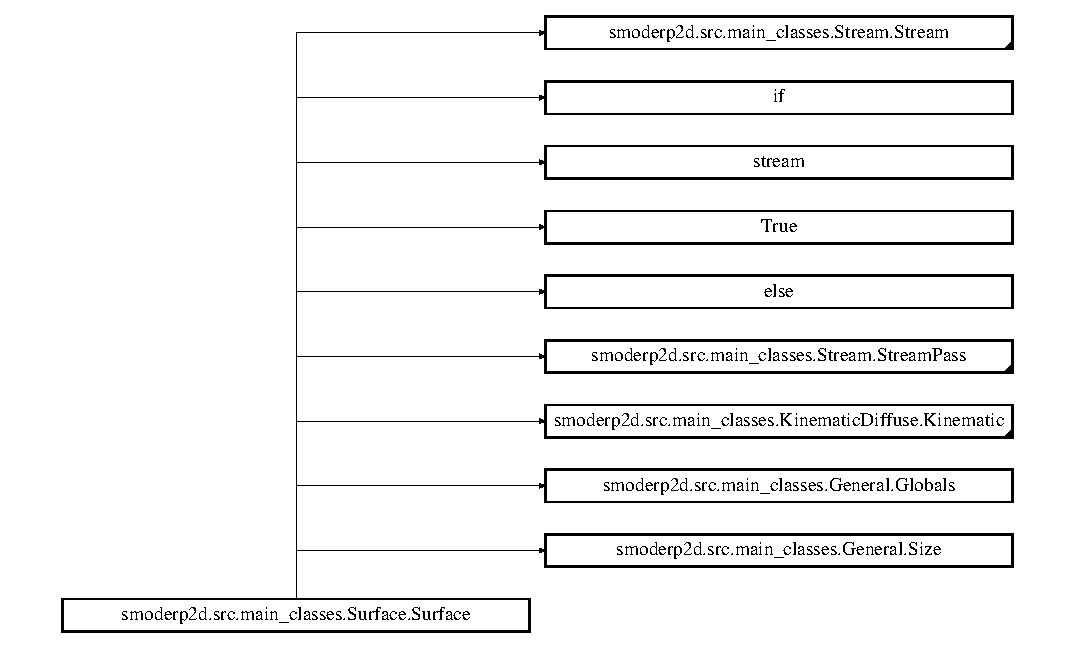
\includegraphics[height=8.259586cm]{d0/d80/classsmoderp2d_1_1src_1_1main__classes_1_1Surface_1_1Surface}
\end{center}
\end{figure}
\subsection*{Public Member Functions}
\begin{DoxyCompactItemize}
\item 
\hypertarget{classsmoderp2d_1_1src_1_1main__classes_1_1Surface_1_1Surface_aec5b45550f4b30c9d06d3b29929b8762}{def \hyperlink{classsmoderp2d_1_1src_1_1main__classes_1_1Surface_1_1Surface_aec5b45550f4b30c9d06d3b29929b8762}{\-\_\-\-\_\-init\-\_\-\-\_\-}}\label{classsmoderp2d_1_1src_1_1main__classes_1_1Surface_1_1Surface_aec5b45550f4b30c9d06d3b29929b8762}

\begin{DoxyCompactList}\small\item\em The constructor make all numpy arrays and establish the inflow procedure based on D8 or Multi \hyperlink{namespacesmoderp2d_1_1src_1_1main__classes_1_1Flow}{Flow} Direction Algorithm method. \end{DoxyCompactList}\item 
\hypertarget{classsmoderp2d_1_1src_1_1main__classes_1_1Surface_1_1Surface_aaef794fb6ee3d7681d62cc084c7193bd}{def {\bfseries return\-\_\-str\-\_\-vals}}\label{classsmoderp2d_1_1src_1_1main__classes_1_1Surface_1_1Surface_aaef794fb6ee3d7681d62cc084c7193bd}

\end{DoxyCompactItemize}
\subsection*{Public Attributes}
\begin{DoxyCompactItemize}
\item 
\hypertarget{classsmoderp2d_1_1src_1_1main__classes_1_1Surface_1_1Surface_aa7c6b79c82e4fdc3c10618352f6f8a95}{{\bfseries n}}\label{classsmoderp2d_1_1src_1_1main__classes_1_1Surface_1_1Surface_aa7c6b79c82e4fdc3c10618352f6f8a95}

\item 
\hypertarget{classsmoderp2d_1_1src_1_1main__classes_1_1Surface_1_1Surface_a7e6c8ba706c0e4a66c5cf9c6411d97f5}{{\bfseries arr}}\label{classsmoderp2d_1_1src_1_1main__classes_1_1Surface_1_1Surface_a7e6c8ba706c0e4a66c5cf9c6411d97f5}

\item 
\hypertarget{classsmoderp2d_1_1src_1_1main__classes_1_1Surface_1_1Surface_a65f67746247e945119a01f15d10cf78c}{{\bfseries r}}\label{classsmoderp2d_1_1src_1_1main__classes_1_1Surface_1_1Surface_a65f67746247e945119a01f15d10cf78c}

\item 
\hypertarget{classsmoderp2d_1_1src_1_1main__classes_1_1Surface_1_1Surface_a6af217c6e409f4f36839b469c70e537f}{{\bfseries c}}\label{classsmoderp2d_1_1src_1_1main__classes_1_1Surface_1_1Surface_a6af217c6e409f4f36839b469c70e537f}

\item 
\hypertarget{classsmoderp2d_1_1src_1_1main__classes_1_1Surface_1_1Surface_a582cc99afa50aa905ee83b83e88f1300}{{\bfseries rill\-\_\-computing}}\label{classsmoderp2d_1_1src_1_1main__classes_1_1Surface_1_1Surface_a582cc99afa50aa905ee83b83e88f1300}

\end{DoxyCompactItemize}
\subsection*{Additional Inherited Members}


\subsection{Detailed Description}
Documentation for a class \hyperlink{classsmoderp2d_1_1src_1_1main__classes_1_1Surface_1_1Surface}{Surface}. 

Class \hyperlink{classsmoderp2d_1_1src_1_1main__classes_1_1Surface_1_1Surface}{Surface} contains data and methods to calculate the surface and rill runoff 

Definition at line 82 of file Surface.\-py.



The documentation for this class was generated from the following file\-:\begin{DoxyCompactItemize}
\item 
smoderp2d/src/main\-\_\-classes/Surface.\-py\end{DoxyCompactItemize}

\hypertarget{classsmoderp2d_1_1src_1_1tools_1_1times__prt_1_1TimesPrt}{\section{smoderp2d.\-src.\-tools.\-times\-\_\-prt.\-Times\-Prt Class Reference}
\label{classsmoderp2d_1_1src_1_1tools_1_1times__prt_1_1TimesPrt}\index{smoderp2d.\-src.\-tools.\-times\-\_\-prt.\-Times\-Prt@{smoderp2d.\-src.\-tools.\-times\-\_\-prt.\-Times\-Prt}}
}
\subsection*{Public Member Functions}
\begin{DoxyCompactItemize}
\item 
\hypertarget{classsmoderp2d_1_1src_1_1tools_1_1times__prt_1_1TimesPrt_a5e31ebdc20a63410a700b37e28145aaa}{def {\bfseries \-\_\-\-\_\-init\-\_\-\-\_\-}}\label{classsmoderp2d_1_1src_1_1tools_1_1times__prt_1_1TimesPrt_a5e31ebdc20a63410a700b37e28145aaa}

\item 
\hypertarget{classsmoderp2d_1_1src_1_1tools_1_1times__prt_1_1TimesPrt_a9bdc7e120830fe25329f92cdc8bef5f1}{def {\bfseries prt}}\label{classsmoderp2d_1_1src_1_1tools_1_1times__prt_1_1TimesPrt_a9bdc7e120830fe25329f92cdc8bef5f1}

\item 
\hypertarget{classsmoderp2d_1_1src_1_1tools_1_1times__prt_1_1TimesPrt_a5e31ebdc20a63410a700b37e28145aaa}{def {\bfseries \-\_\-\-\_\-init\-\_\-\-\_\-}}\label{classsmoderp2d_1_1src_1_1tools_1_1times__prt_1_1TimesPrt_a5e31ebdc20a63410a700b37e28145aaa}

\item 
\hypertarget{classsmoderp2d_1_1src_1_1tools_1_1times__prt_1_1TimesPrt_a9bdc7e120830fe25329f92cdc8bef5f1}{def {\bfseries prt}}\label{classsmoderp2d_1_1src_1_1tools_1_1times__prt_1_1TimesPrt_a9bdc7e120830fe25329f92cdc8bef5f1}

\end{DoxyCompactItemize}
\subsection*{Public Attributes}
\begin{DoxyCompactItemize}
\item 
\hypertarget{classsmoderp2d_1_1src_1_1tools_1_1times__prt_1_1TimesPrt_a169eae410f43ff85b68f5bf5306e3acb}{{\bfseries f\-Times}}\label{classsmoderp2d_1_1src_1_1tools_1_1times__prt_1_1TimesPrt_a169eae410f43ff85b68f5bf5306e3acb}

\item 
\hypertarget{classsmoderp2d_1_1src_1_1tools_1_1times__prt_1_1TimesPrt_ad38d98b1f1e7bb24eccb06acb8252856}{{\bfseries outsubrid}}\label{classsmoderp2d_1_1src_1_1tools_1_1times__prt_1_1TimesPrt_ad38d98b1f1e7bb24eccb06acb8252856}

\item 
\hypertarget{classsmoderp2d_1_1src_1_1tools_1_1times__prt_1_1TimesPrt_a4f3c75594d01d3d5dbee4244edd4fb64}{{\bfseries times}}\label{classsmoderp2d_1_1src_1_1tools_1_1times__prt_1_1TimesPrt_a4f3c75594d01d3d5dbee4244edd4fb64}

\end{DoxyCompactItemize}


\subsection{Detailed Description}


Definition at line 13 of file times\-\_\-prt.\-py.



The documentation for this class was generated from the following file\-:\begin{DoxyCompactItemize}
\item 
smoderp2d/src/tools/times\-\_\-prt.\-py\end{DoxyCompactItemize}

\hypertarget{classsmoderp2d_1_1src_1_1time__step_1_1TimeStep}{\section{smoderp2d.\-src.\-time\-\_\-step.\-Time\-Step Class Reference}
\label{classsmoderp2d_1_1src_1_1time__step_1_1TimeStep}\index{smoderp2d.\-src.\-time\-\_\-step.\-Time\-Step@{smoderp2d.\-src.\-time\-\_\-step.\-Time\-Step}}
}


Class manages the one time step operation.  


\subsection*{Public Member Functions}
\begin{DoxyCompactItemize}
\item 
\hypertarget{classsmoderp2d_1_1src_1_1time__step_1_1TimeStep_ae256e735639ddea75ec60804b91d8d7a}{def {\bfseries do\-\_\-flow}}\label{classsmoderp2d_1_1src_1_1time__step_1_1TimeStep_ae256e735639ddea75ec60804b91d8d7a}

\item 
\hypertarget{classsmoderp2d_1_1src_1_1time__step_1_1TimeStep_af9c42120993834afb4318d35cbedd47e}{def {\bfseries do\-\_\-next\-\_\-h}}\label{classsmoderp2d_1_1src_1_1time__step_1_1TimeStep_af9c42120993834afb4318d35cbedd47e}

\end{DoxyCompactItemize}


\subsection{Detailed Description}
Class manages the one time step operation. 

the class also contains methods to store the important arrays to reload that if the time step is adjusted 

The documentation for this class was generated from the following file\-:\begin{DoxyCompactItemize}
\item 
smoderp2d/src/time\-\_\-step.\-py\end{DoxyCompactItemize}

\hypertarget{classsmoderp2d_1_1src_1_1main__classes_1_1Vegetation_1_1VegArrs}{\section{smoderp2d.\-src.\-main\-\_\-classes.\-Vegetation.\-Veg\-Arrs Class Reference}
\label{classsmoderp2d_1_1src_1_1main__classes_1_1Vegetation_1_1VegArrs}\index{smoderp2d.\-src.\-main\-\_\-classes.\-Vegetation.\-Veg\-Arrs@{smoderp2d.\-src.\-main\-\_\-classes.\-Vegetation.\-Veg\-Arrs}}
}
\subsection*{Public Member Functions}
\begin{DoxyCompactItemize}
\item 
\hypertarget{classsmoderp2d_1_1src_1_1main__classes_1_1Vegetation_1_1VegArrs_aa10c88b822b18c2d6b19954c8d2cc8dd}{def {\bfseries \-\_\-\-\_\-init\-\_\-\-\_\-}}\label{classsmoderp2d_1_1src_1_1main__classes_1_1Vegetation_1_1VegArrs_aa10c88b822b18c2d6b19954c8d2cc8dd}

\end{DoxyCompactItemize}
\subsection*{Public Attributes}
\begin{DoxyCompactItemize}
\item 
\hypertarget{classsmoderp2d_1_1src_1_1main__classes_1_1Vegetation_1_1VegArrs_a16b63c13be70c6dad44bf2e0773c9ad2}{{\bfseries veg\-\_\-true}}\label{classsmoderp2d_1_1src_1_1main__classes_1_1Vegetation_1_1VegArrs_a16b63c13be70c6dad44bf2e0773c9ad2}

\item 
\hypertarget{classsmoderp2d_1_1src_1_1main__classes_1_1Vegetation_1_1VegArrs_ad7a7ce1bf3b553b5830e26e024bfc80f}{{\bfseries ppl}}\label{classsmoderp2d_1_1src_1_1main__classes_1_1Vegetation_1_1VegArrs_ad7a7ce1bf3b553b5830e26e024bfc80f}

\item 
\hypertarget{classsmoderp2d_1_1src_1_1main__classes_1_1Vegetation_1_1VegArrs_a76bc6f578cf57962308c935b08fdcade}{{\bfseries pi}}\label{classsmoderp2d_1_1src_1_1main__classes_1_1Vegetation_1_1VegArrs_a76bc6f578cf57962308c935b08fdcade}

\end{DoxyCompactItemize}


\subsection{Detailed Description}


Definition at line 9 of file Vegetation.\-py.



The documentation for this class was generated from the following file\-:\begin{DoxyCompactItemize}
\item 
smoderp2d/src/main\-\_\-classes/Vegetation.\-py\end{DoxyCompactItemize}

\hypertarget{classsmoderp2d_1_1src_1_1main__classes_1_1Vegetation_1_1Vegetation}{\section{smoderp2d.\-src.\-main\-\_\-classes.\-Vegetation.\-Vegetation Class Reference}
\label{classsmoderp2d_1_1src_1_1main__classes_1_1Vegetation_1_1Vegetation}\index{smoderp2d.\-src.\-main\-\_\-classes.\-Vegetation.\-Vegetation@{smoderp2d.\-src.\-main\-\_\-classes.\-Vegetation.\-Vegetation}}
}


Documentation for a class.  


Inheritance diagram for smoderp2d.\-src.\-main\-\_\-classes.\-Vegetation.\-Vegetation\-:\begin{figure}[H]
\begin{center}
\leavevmode
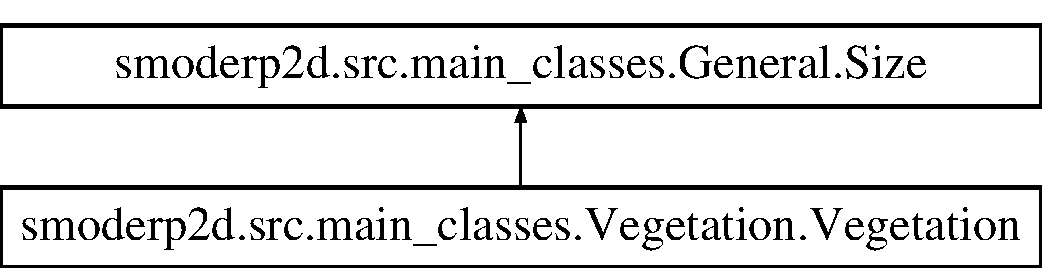
\includegraphics[height=2.000000cm]{d7/d67/classsmoderp2d_1_1src_1_1main__classes_1_1Vegetation_1_1Vegetation}
\end{center}
\end{figure}
\subsection*{Public Member Functions}
\begin{DoxyCompactItemize}
\item 
def \hyperlink{classsmoderp2d_1_1src_1_1main__classes_1_1Vegetation_1_1Vegetation_a43109cd6b3a251504b55454a9a838ec3}{\-\_\-\-\_\-init\-\_\-\-\_\-}
\begin{DoxyCompactList}\small\item\em The constructor. \end{DoxyCompactList}\end{DoxyCompactItemize}
\subsection*{Public Attributes}
\begin{DoxyCompactItemize}
\item 
\hypertarget{classsmoderp2d_1_1src_1_1main__classes_1_1Vegetation_1_1Vegetation_a9593101bb8240bc05a0f96b25a584c61}{{\bfseries n}}\label{classsmoderp2d_1_1src_1_1main__classes_1_1Vegetation_1_1Vegetation_a9593101bb8240bc05a0f96b25a584c61}

\item 
\hypertarget{classsmoderp2d_1_1src_1_1main__classes_1_1Vegetation_1_1Vegetation_a507eb051e0057baa26987568f2cae514}{{\bfseries arr}}\label{classsmoderp2d_1_1src_1_1main__classes_1_1Vegetation_1_1Vegetation_a507eb051e0057baa26987568f2cae514}

\end{DoxyCompactItemize}


\subsection{Detailed Description}
Documentation for a class. 

More details. 

Definition at line 19 of file Vegetation.\-py.



\subsection{Constructor \& Destructor Documentation}
\hypertarget{classsmoderp2d_1_1src_1_1main__classes_1_1Vegetation_1_1Vegetation_a43109cd6b3a251504b55454a9a838ec3}{\index{smoderp2d\-::src\-::main\-\_\-classes\-::\-Vegetation\-::\-Vegetation@{smoderp2d\-::src\-::main\-\_\-classes\-::\-Vegetation\-::\-Vegetation}!\-\_\-\-\_\-init\-\_\-\-\_\-@{\-\_\-\-\_\-init\-\_\-\-\_\-}}
\index{\-\_\-\-\_\-init\-\_\-\-\_\-@{\-\_\-\-\_\-init\-\_\-\-\_\-}!smoderp2d::src::main_classes::Vegetation::Vegetation@{smoderp2d\-::src\-::main\-\_\-classes\-::\-Vegetation\-::\-Vegetation}}
\subsubsection[{\-\_\-\-\_\-init\-\_\-\-\_\-}]{\setlength{\rightskip}{0pt plus 5cm}def smoderp2d.\-src.\-main\-\_\-classes.\-Vegetation.\-Vegetation.\-\_\-\-\_\-init\-\_\-\-\_\- (
\begin{DoxyParamCaption}
\item[{}]{self, }
\item[{}]{r, }
\item[{}]{c, }
\item[{}]{mat\-\_\-ppl, }
\item[{}]{mat\-\_\-pi}
\end{DoxyParamCaption}
)}}\label{classsmoderp2d_1_1src_1_1main__classes_1_1Vegetation_1_1Vegetation_a43109cd6b3a251504b55454a9a838ec3}


The constructor. 



Definition at line 23 of file Vegetation.\-py.


\begin{DoxyCode}
23 
24   \textcolor{keyword}{def }\hyperlink{classsmoderp2d_1_1src_1_1main__classes_1_1Vegetation_1_1Vegetation_a43109cd6b3a251504b55454a9a838ec3}{\_\_init\_\_}(self,r,c,mat\_ppl,mat\_pi):
25 
26     self.\hyperlink{classsmoderp2d_1_1src_1_1main__classes_1_1Vegetation_1_1Vegetation_a9593101bb8240bc05a0f96b25a584c61}{n} = 3
27     self.\hyperlink{classsmoderp2d_1_1src_1_1main__classes_1_1Vegetation_1_1Vegetation_a507eb051e0057baa26987568f2cae514}{arr} = np.empty((r,c), dtype=object)
28 
29     \textcolor{keywordflow}{for} i \textcolor{keywordflow}{in} range(r):
30       \textcolor{keywordflow}{for} j \textcolor{keywordflow}{in} range(c):
31         self.\hyperlink{classsmoderp2d_1_1src_1_1main__classes_1_1Vegetation_1_1Vegetation_a507eb051e0057baa26987568f2cae514}{arr}[i][j] = \hyperlink{classsmoderp2d_1_1src_1_1main__classes_1_1Vegetation_1_1VegArrs}{VegArrs}(0,mat\_ppl[i][j],mat\_pi[i][j])
32         
33         
34         
        \end{DoxyCode}


The documentation for this class was generated from the following file\-:\begin{DoxyCompactItemize}
\item 
smoderp2d/src/main\-\_\-classes/Vegetation.\-py\end{DoxyCompactItemize}

\hypertarget{classsmoderp2d_1_1src_1_1stream__functions_1_1stream__preparation_1_1ZeroSlopeError}{\section{smoderp2d.\-src.\-stream\-\_\-functions.\-stream\-\_\-preparation.\-Zero\-Slope\-Error Class Reference}
\label{classsmoderp2d_1_1src_1_1stream__functions_1_1stream__preparation_1_1ZeroSlopeError}\index{smoderp2d.\-src.\-stream\-\_\-functions.\-stream\-\_\-preparation.\-Zero\-Slope\-Error@{smoderp2d.\-src.\-stream\-\_\-functions.\-stream\-\_\-preparation.\-Zero\-Slope\-Error}}
}
Inheritance diagram for smoderp2d.\-src.\-stream\-\_\-functions.\-stream\-\_\-preparation.\-Zero\-Slope\-Error\-:\begin{figure}[H]
\begin{center}
\leavevmode
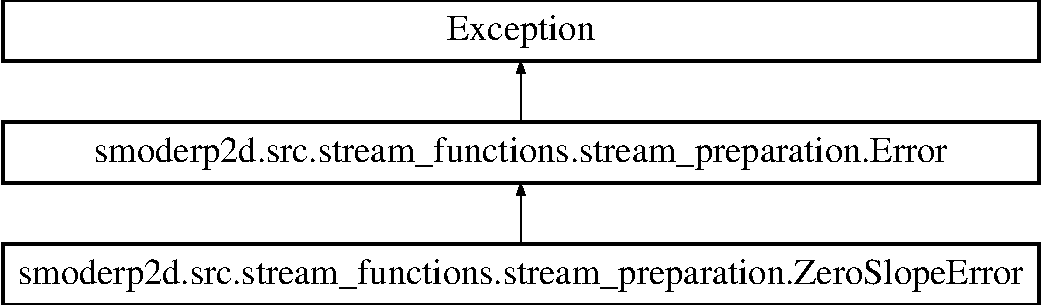
\includegraphics[height=3.000000cm]{d1/d84/classsmoderp2d_1_1src_1_1stream__functions_1_1stream__preparation_1_1ZeroSlopeError}
\end{center}
\end{figure}
\subsection*{Public Member Functions}
\begin{DoxyCompactItemize}
\item 
\hypertarget{classsmoderp2d_1_1src_1_1stream__functions_1_1stream__preparation_1_1ZeroSlopeError_ac2efe0eada14a4d9333fc44640e1a71d}{def {\bfseries \-\_\-\-\_\-init\-\_\-\-\_\-}}\label{classsmoderp2d_1_1src_1_1stream__functions_1_1stream__preparation_1_1ZeroSlopeError_ac2efe0eada14a4d9333fc44640e1a71d}

\item 
\hypertarget{classsmoderp2d_1_1src_1_1stream__functions_1_1stream__preparation_1_1ZeroSlopeError_a6f2e5c2a0a2d320a5dc9d4f5cfdcdb34}{def {\bfseries \-\_\-\-\_\-str\-\_\-\-\_\-}}\label{classsmoderp2d_1_1src_1_1stream__functions_1_1stream__preparation_1_1ZeroSlopeError_a6f2e5c2a0a2d320a5dc9d4f5cfdcdb34}

\end{DoxyCompactItemize}
\subsection*{Public Attributes}
\begin{DoxyCompactItemize}
\item 
\hypertarget{classsmoderp2d_1_1src_1_1stream__functions_1_1stream__preparation_1_1ZeroSlopeError_ab41f8e7b39300db9de9b662eee2740be}{{\bfseries msg}}\label{classsmoderp2d_1_1src_1_1stream__functions_1_1stream__preparation_1_1ZeroSlopeError_ab41f8e7b39300db9de9b662eee2740be}

\end{DoxyCompactItemize}


\subsection{Detailed Description}
\begin{DoxyVerb}Exception raised for zero slope of a reach.

Attributes:
    msg  -- explanation of the error
\end{DoxyVerb}
 

Definition at line 38 of file stream\-\_\-preparation.\-py.



The documentation for this class was generated from the following file\-:\begin{DoxyCompactItemize}
\item 
smoderp2d/src/stream\-\_\-functions/stream\-\_\-preparation.\-py\end{DoxyCompactItemize}

%--- End generated contents ---

% Index
\newpage
\phantomsection
\addcontentsline{toc}{chapter}{Index}
\printindex

\end{document}
